\documentclass[twoside]{book}

% Packages required by doxygen
\usepackage{calc}
\usepackage{doxygen}
\usepackage{graphicx}
\usepackage[utf8]{inputenc}
\usepackage{makeidx}
\usepackage{multicol}
\usepackage{multirow}
\usepackage{textcomp}
\usepackage[table]{xcolor}

% NLS support packages
\usepackage{polski}
\usepackage[T1]{fontenc}

% Font selection
\usepackage[T1]{fontenc}
\usepackage{mathptmx}
\usepackage[scaled=.90]{helvet}
\usepackage{courier}
\usepackage{amssymb}
\usepackage{sectsty}
\renewcommand{\familydefault}{\sfdefault}
\allsectionsfont{%
  \fontseries{bc}\selectfont%
  \color{darkgray}%
}
\renewcommand{\DoxyLabelFont}{%
  \fontseries{bc}\selectfont%
  \color{darkgray}%
}

% Page & text layout
\usepackage{geometry}
\geometry{%
  a4paper,%
  top=2.5cm,%
  bottom=2.5cm,%
  left=2.5cm,%
  right=2.5cm%
}
\tolerance=750
\hfuzz=15pt
\hbadness=750
\setlength{\emergencystretch}{15pt}
\setlength{\parindent}{0cm}
\setlength{\parskip}{0.2cm}
\makeatletter
\renewcommand{\paragraph}{%
  \@startsection{paragraph}{4}{0ex}{-1.0ex}{1.0ex}{%
    \normalfont\normalsize\bfseries\SS@parafont%
  }%
}
\renewcommand{\subparagraph}{%
  \@startsection{subparagraph}{5}{0ex}{-1.0ex}{1.0ex}{%
    \normalfont\normalsize\bfseries\SS@subparafont%
  }%
}
\makeatother

% Headers & footers
\usepackage{fancyhdr}
\pagestyle{fancyplain}
\fancyhead[LE]{\fancyplain{}{\bfseries\thepage}}
\fancyhead[CE]{\fancyplain{}{}}
\fancyhead[RE]{\fancyplain{}{\bfseries\leftmark}}
\fancyhead[LO]{\fancyplain{}{\bfseries\rightmark}}
\fancyhead[CO]{\fancyplain{}{}}
\fancyhead[RO]{\fancyplain{}{\bfseries\thepage}}
\fancyfoot[LE]{\fancyplain{}{}}
\fancyfoot[CE]{\fancyplain{}{}}
\fancyfoot[RE]{\fancyplain{}{\bfseries\scriptsize Wygenerowano Pt, 13 cze 2014 20\-:48\-:29 dla Gra programem Doxygen }}
\fancyfoot[LO]{\fancyplain{}{\bfseries\scriptsize Wygenerowano Pt, 13 cze 2014 20\-:48\-:29 dla Gra programem Doxygen }}
\fancyfoot[CO]{\fancyplain{}{}}
\fancyfoot[RO]{\fancyplain{}{}}
\renewcommand{\footrulewidth}{0.4pt}
\renewcommand{\chaptermark}[1]{%
  \markboth{#1}{}%
}
\renewcommand{\sectionmark}[1]{%
  \markright{\thesection\ #1}%
}

% Indices & bibliography
\usepackage{natbib}
\usepackage[titles]{tocloft}
\setcounter{tocdepth}{3}
\setcounter{secnumdepth}{5}
\makeindex

% Hyperlinks (required, but should be loaded last)
\usepackage{ifpdf}
\ifpdf
  \usepackage[pdftex,pagebackref=true]{hyperref}
\else
  \usepackage[ps2pdf,pagebackref=true]{hyperref}
\fi
\hypersetup{%
  colorlinks=true,%
  linkcolor=blue,%
  citecolor=blue,%
  unicode%
}

% Custom commands
\newcommand{\clearemptydoublepage}{%
  \newpage{\pagestyle{empty}\cleardoublepage}%
}


%===== C O N T E N T S =====

\begin{document}

% Titlepage & ToC
\hypersetup{pageanchor=false}
\pagenumbering{roman}
\begin{titlepage}
\vspace*{7cm}
\begin{center}%
{\Large Gra }\\
\vspace*{1cm}
{\large Wygenerowano przez Doxygen 1.8.6}\\
\vspace*{0.5cm}
{\small Pt, 13 cze 2014 20:48:29}\\
\end{center}
\end{titlepage}
\clearemptydoublepage
\tableofcontents
\clearemptydoublepage
\pagenumbering{arabic}
\hypersetup{pageanchor=true}

%--- Begin generated contents ---
\chapter{Indeks przestrzeni nazw}
\section{Lista przestrzeni nazw}
Tutaj znajdują się wszystkie przestrzenie nazw wraz z ich krótkimi opisami\-:\begin{DoxyCompactList}
\item\contentsline{section}{\hyperlink{namespaceUi}{Ui} }{\pageref{db/d3c/namespaceUi}}{}
\end{DoxyCompactList}

\chapter{Indeks hierarchiczny}
\section{Hierarchia klas}
Ta lista dziedziczenia posortowana jest z grubsza, choć nie całkowicie, alfabetycznie\-:\begin{DoxyCompactList}
\item \contentsline{section}{Figura}{\pageref{d9/d07/classFigura}}{}
\begin{DoxyCompactList}
\item \contentsline{section}{Kolo}{\pageref{d6/d1e/classKolo}}{}
\item \contentsline{section}{Kolo}{\pageref{d6/d1e/classKolo}}{}
\item \contentsline{section}{Kwadrat}{\pageref{d4/d2c/classKwadrat}}{}
\item \contentsline{section}{Kwadrat}{\pageref{d4/d2c/classKwadrat}}{}
\item \contentsline{section}{Trojkat}{\pageref{d4/d42/classTrojkat}}{}
\item \contentsline{section}{Trojkat}{\pageref{d4/d42/classTrojkat}}{}
\end{DoxyCompactList}
\item \contentsline{section}{Odcinek}{\pageref{d3/d0b/classOdcinek}}{}
\item \contentsline{section}{Poziomy}{\pageref{d5/d84/classPoziomy}}{}
\item Q\-Dialog\begin{DoxyCompactList}
\item \contentsline{section}{Dialog}{\pageref{dc/d06/classDialog}}{}
\item \contentsline{section}{Dialog2}{\pageref{d9/dde/classDialog2}}{}
\end{DoxyCompactList}
\item Q\-G\-L\-Widget\begin{DoxyCompactList}
\item \contentsline{section}{My\-G\-L\-Widget}{\pageref{d0/da8/classMyGLWidget}}{}
\item \contentsline{section}{My\-G\-L\-Widget}{\pageref{d0/da8/classMyGLWidget}}{}
\end{DoxyCompactList}
\item Q\-Main\-Window\begin{DoxyCompactList}
\item \contentsline{section}{Main\-Window}{\pageref{d6/d1a/classMainWindow}}{}
\item \contentsline{section}{Main\-Window}{\pageref{d6/d1a/classMainWindow}}{}
\end{DoxyCompactList}
\item \contentsline{section}{qt\-\_\-meta\-\_\-stringdata\-\_\-\-Dialog2\-\_\-t}{\pageref{dc/d7d/structqt__meta__stringdata__Dialog2__t}}{}
\item \contentsline{section}{qt\-\_\-meta\-\_\-stringdata\-\_\-\-Dialog\-\_\-t}{\pageref{da/d4d/structqt__meta__stringdata__Dialog__t}}{}
\item \contentsline{section}{qt\-\_\-meta\-\_\-stringdata\-\_\-\-Main\-Window\-\_\-t}{\pageref{db/d49/structqt__meta__stringdata__MainWindow__t}}{}
\item \contentsline{section}{qt\-\_\-meta\-\_\-stringdata\-\_\-\-My\-G\-L\-Widget\-\_\-t}{\pageref{d7/dce/structqt__meta__stringdata__MyGLWidget__t}}{}
\item \contentsline{section}{Ui\-\_\-\-Dialog}{\pageref{d7/d7b/classUi__Dialog}}{}
\begin{DoxyCompactList}
\item \contentsline{section}{Ui\-:\-:Dialog}{\pageref{df/d9e/classUi_1_1Dialog}}{}
\end{DoxyCompactList}
\item \contentsline{section}{Ui\-\_\-\-Dialog2}{\pageref{d6/d6d/classUi__Dialog2}}{}
\begin{DoxyCompactList}
\item \contentsline{section}{Ui\-:\-:Dialog2}{\pageref{dd/d3c/classUi_1_1Dialog2}}{}
\end{DoxyCompactList}
\item \contentsline{section}{Ui\-\_\-\-Main\-Window}{\pageref{d5/d3f/classUi__MainWindow}}{}
\begin{DoxyCompactList}
\item \contentsline{section}{Ui\-:\-:Main\-Window}{\pageref{d9/dbd/classUi_1_1MainWindow}}{}
\item \contentsline{section}{Ui\-:\-:Main\-Window}{\pageref{d9/dbd/classUi_1_1MainWindow}}{}
\end{DoxyCompactList}
\end{DoxyCompactList}

\chapter{Indeks klas}
\section{Lista klas}
Tutaj znajdują się klasy, struktury, unie i interfejsy wraz z ich krótkimi opisami\-:\begin{DoxyCompactList}
\item\contentsline{section}{\hyperlink{classDialog}{Dialog} \\*Okno Dialogowe }{\pageref{dc/d06/classDialog}}{}
\item\contentsline{section}{\hyperlink{classUi_1_1Dialog}{Ui\-::\-Dialog} }{\pageref{df/d9e/classUi_1_1Dialog}}{}
\item\contentsline{section}{\hyperlink{classDialog2}{Dialog2} \\*Okno Dialogowe }{\pageref{d9/dde/classDialog2}}{}
\item\contentsline{section}{\hyperlink{classUi_1_1Dialog2}{Ui\-::\-Dialog2} }{\pageref{dd/d3c/classUi_1_1Dialog2}}{}
\item\contentsline{section}{\hyperlink{classFigura}{Figura} \\*The \hyperlink{classFigura}{Figura} class }{\pageref{d9/d07/classFigura}}{}
\item\contentsline{section}{\hyperlink{classKolo}{Kolo} }{\pageref{d6/d1e/classKolo}}{}
\item\contentsline{section}{\hyperlink{classKwadrat}{Kwadrat} }{\pageref{d4/d2c/classKwadrat}}{}
\item\contentsline{section}{\hyperlink{classUi_1_1MainWindow}{Ui\-::\-Main\-Window} }{\pageref{d9/dbd/classUi_1_1MainWindow}}{}
\item\contentsline{section}{\hyperlink{classMainWindow}{Main\-Window} }{\pageref{d6/d1a/classMainWindow}}{}
\item\contentsline{section}{\hyperlink{classMyGLWidget}{My\-G\-L\-Widget} }{\pageref{d0/da8/classMyGLWidget}}{}
\item\contentsline{section}{\hyperlink{classOdcinek}{Odcinek} }{\pageref{d3/d0b/classOdcinek}}{}
\item\contentsline{section}{\hyperlink{classPoziomy}{Poziomy} }{\pageref{d5/d84/classPoziomy}}{}
\item\contentsline{section}{\hyperlink{structqt__meta__stringdata__Dialog2__t}{qt\-\_\-meta\-\_\-stringdata\-\_\-\-Dialog2\-\_\-t} }{\pageref{dc/d7d/structqt__meta__stringdata__Dialog2__t}}{}
\item\contentsline{section}{\hyperlink{structqt__meta__stringdata__Dialog__t}{qt\-\_\-meta\-\_\-stringdata\-\_\-\-Dialog\-\_\-t} }{\pageref{da/d4d/structqt__meta__stringdata__Dialog__t}}{}
\item\contentsline{section}{\hyperlink{structqt__meta__stringdata__MainWindow__t}{qt\-\_\-meta\-\_\-stringdata\-\_\-\-Main\-Window\-\_\-t} }{\pageref{db/d49/structqt__meta__stringdata__MainWindow__t}}{}
\item\contentsline{section}{\hyperlink{structqt__meta__stringdata__MyGLWidget__t}{qt\-\_\-meta\-\_\-stringdata\-\_\-\-My\-G\-L\-Widget\-\_\-t} }{\pageref{d7/dce/structqt__meta__stringdata__MyGLWidget__t}}{}
\item\contentsline{section}{\hyperlink{classTrojkat}{Trojkat} }{\pageref{d4/d42/classTrojkat}}{}
\item\contentsline{section}{\hyperlink{classUi__Dialog}{Ui\-\_\-\-Dialog} }{\pageref{d7/d7b/classUi__Dialog}}{}
\item\contentsline{section}{\hyperlink{classUi__Dialog2}{Ui\-\_\-\-Dialog2} }{\pageref{d6/d6d/classUi__Dialog2}}{}
\item\contentsline{section}{\hyperlink{classUi__MainWindow}{Ui\-\_\-\-Main\-Window} }{\pageref{d5/d3f/classUi__MainWindow}}{}
\end{DoxyCompactList}

\chapter{Indeks plików}
\section{Lista plików}
Tutaj znajduje się lista wszystkich plików z ich krótkimi opisami\-:\begin{DoxyCompactList}
\item\contentsline{section}{Gra\-Figury/\hyperlink{dialog_8cpp}{dialog.\-cpp} }{\pageref{de/dfa/dialog_8cpp}}{}
\item\contentsline{section}{Gra\-Figury/\hyperlink{dialog_8h}{dialog.\-h} }{\pageref{d1/dc9/dialog_8h}}{}
\item\contentsline{section}{Gra\-Figury/\hyperlink{dialog2_8cpp}{dialog2.\-cpp} }{\pageref{dd/d57/dialog2_8cpp}}{}
\item\contentsline{section}{Gra\-Figury/\hyperlink{dialog2_8h}{dialog2.\-h} }{\pageref{d5/ddf/dialog2_8h}}{}
\item\contentsline{section}{Gra\-Figury/\hyperlink{GraFigury_2figura_8cpp}{figura.\-cpp} }{\pageref{d1/d95/GraFigury_2figura_8cpp}}{}
\item\contentsline{section}{Gra\-Figury/\hyperlink{GraFigury_2figura_8h}{figura.\-h} }{\pageref{d1/db1/GraFigury_2figura_8h}}{}
\item\contentsline{section}{Gra\-Figury/\hyperlink{GraFigury_2kolo_8cpp}{kolo.\-cpp} }{\pageref{d6/d63/GraFigury_2kolo_8cpp}}{}
\item\contentsline{section}{Gra\-Figury/\hyperlink{GraFigury_2kolo_8h}{kolo.\-h} }{\pageref{da/d77/GraFigury_2kolo_8h}}{}
\item\contentsline{section}{Gra\-Figury/\hyperlink{GraFigury_2kwadrat_8cpp}{kwadrat.\-cpp} }{\pageref{d5/d27/GraFigury_2kwadrat_8cpp}}{}
\item\contentsline{section}{Gra\-Figury/\hyperlink{GraFigury_2kwadrat_8h}{kwadrat.\-h} }{\pageref{df/d0d/GraFigury_2kwadrat_8h}}{}
\item\contentsline{section}{Gra\-Figury/\hyperlink{GraFigury_2main_8cpp}{main.\-cpp} }{\pageref{d2/d20/GraFigury_2main_8cpp}}{}
\item\contentsline{section}{Gra\-Figury/\hyperlink{GraFigury_2mainwindow_8cpp}{mainwindow.\-cpp} }{\pageref{db/d7e/GraFigury_2mainwindow_8cpp}}{}
\item\contentsline{section}{Gra\-Figury/\hyperlink{GraFigury_2mainwindow_8h}{mainwindow.\-h} }{\pageref{d9/dd3/GraFigury_2mainwindow_8h}}{}
\item\contentsline{section}{Gra\-Figury/\hyperlink{moc__dialog_8cpp}{moc\-\_\-dialog.\-cpp} }{\pageref{d2/d08/moc__dialog_8cpp}}{}
\item\contentsline{section}{Gra\-Figury/\hyperlink{moc__dialog2_8cpp}{moc\-\_\-dialog2.\-cpp} }{\pageref{d3/df3/moc__dialog2_8cpp}}{}
\item\contentsline{section}{Gra\-Figury/\hyperlink{GraFigury_2moc__mainwindow_8cpp}{moc\-\_\-mainwindow.\-cpp} }{\pageref{da/ddd/GraFigury_2moc__mainwindow_8cpp}}{}
\item\contentsline{section}{Gra\-Figury/\hyperlink{moc__myglwidget_8cpp}{moc\-\_\-myglwidget.\-cpp} }{\pageref{d4/d47/moc__myglwidget_8cpp}}{}
\item\contentsline{section}{Gra\-Figury/\hyperlink{GraFigury_2myglwidget_8cpp}{myglwidget.\-cpp} }{\pageref{d9/da8/GraFigury_2myglwidget_8cpp}}{}
\item\contentsline{section}{Gra\-Figury/\hyperlink{GraFigury_2myglwidget_8h}{myglwidget.\-h} }{\pageref{d6/da3/GraFigury_2myglwidget_8h}}{}
\item\contentsline{section}{Gra\-Figury/\hyperlink{GraFigury_2odcinek_8cpp}{odcinek.\-cpp} }{\pageref{d9/d3d/GraFigury_2odcinek_8cpp}}{}
\item\contentsline{section}{Gra\-Figury/\hyperlink{GraFigury_2odcinek_8h}{odcinek.\-h} }{\pageref{dd/d9a/GraFigury_2odcinek_8h}}{}
\item\contentsline{section}{Gra\-Figury/\hyperlink{GraFigury_2poziomy_8cpp}{poziomy.\-cpp} }{\pageref{df/d36/GraFigury_2poziomy_8cpp}}{}
\item\contentsline{section}{Gra\-Figury/\hyperlink{GraFigury_2poziomy_8h}{poziomy.\-h} }{\pageref{d3/dec/GraFigury_2poziomy_8h}}{}
\item\contentsline{section}{Gra\-Figury/\hyperlink{GraFigury_2trojkat_8cpp}{trojkat.\-cpp} }{\pageref{d5/d00/GraFigury_2trojkat_8cpp}}{}
\item\contentsline{section}{Gra\-Figury/\hyperlink{GraFigury_2trojkat_8h}{trojkat.\-h} }{\pageref{d3/d59/GraFigury_2trojkat_8h}}{}
\item\contentsline{section}{Gra\-Figury/\hyperlink{ui__dialog_8h}{ui\-\_\-dialog.\-h} }{\pageref{d1/d98/ui__dialog_8h}}{}
\item\contentsline{section}{Gra\-Figury/\hyperlink{ui__dialog2_8h}{ui\-\_\-dialog2.\-h} }{\pageref{dc/d20/ui__dialog2_8h}}{}
\item\contentsline{section}{Gra\-Figury/\hyperlink{GraFigury_2ui__mainwindow_8h}{ui\-\_\-mainwindow.\-h} }{\pageref{d1/d40/GraFigury_2ui__mainwindow_8h}}{}
\item\contentsline{section}{Serwer\-Figury/\hyperlink{SerwerFigury_2figura_8cpp}{figura.\-cpp} }{\pageref{dc/da4/SerwerFigury_2figura_8cpp}}{}
\item\contentsline{section}{Serwer\-Figury/\hyperlink{SerwerFigury_2figura_8h}{figura.\-h} }{\pageref{d6/d9e/SerwerFigury_2figura_8h}}{}
\item\contentsline{section}{Serwer\-Figury/\hyperlink{SerwerFigury_2kolo_8cpp}{kolo.\-cpp} }{\pageref{dc/d7b/SerwerFigury_2kolo_8cpp}}{}
\item\contentsline{section}{Serwer\-Figury/\hyperlink{SerwerFigury_2kolo_8h}{kolo.\-h} }{\pageref{dd/d78/SerwerFigury_2kolo_8h}}{}
\item\contentsline{section}{Serwer\-Figury/\hyperlink{SerwerFigury_2kwadrat_8cpp}{kwadrat.\-cpp} }{\pageref{d7/d47/SerwerFigury_2kwadrat_8cpp}}{}
\item\contentsline{section}{Serwer\-Figury/\hyperlink{SerwerFigury_2kwadrat_8h}{kwadrat.\-h} }{\pageref{dc/d21/SerwerFigury_2kwadrat_8h}}{}
\item\contentsline{section}{Serwer\-Figury/\hyperlink{SerwerFigury_2main_8cpp}{main.\-cpp} }{\pageref{de/d64/SerwerFigury_2main_8cpp}}{}
\item\contentsline{section}{Serwer\-Figury/\hyperlink{SerwerFigury_2mainwindow_8cpp}{mainwindow.\-cpp} }{\pageref{df/ded/SerwerFigury_2mainwindow_8cpp}}{}
\item\contentsline{section}{Serwer\-Figury/\hyperlink{SerwerFigury_2mainwindow_8h}{mainwindow.\-h} }{\pageref{d4/da8/SerwerFigury_2mainwindow_8h}}{}
\item\contentsline{section}{Serwer\-Figury/\hyperlink{SerwerFigury_2moc__mainwindow_8cpp}{moc\-\_\-mainwindow.\-cpp} }{\pageref{de/d65/SerwerFigury_2moc__mainwindow_8cpp}}{}
\item\contentsline{section}{Serwer\-Figury/\hyperlink{SerwerFigury_2myglwidget_8cpp}{myglwidget.\-cpp} }{\pageref{dc/d86/SerwerFigury_2myglwidget_8cpp}}{}
\item\contentsline{section}{Serwer\-Figury/\hyperlink{SerwerFigury_2myglwidget_8h}{myglwidget.\-h} }{\pageref{d1/d23/SerwerFigury_2myglwidget_8h}}{}
\item\contentsline{section}{Serwer\-Figury/\hyperlink{SerwerFigury_2odcinek_8cpp}{odcinek.\-cpp} }{\pageref{d2/d48/SerwerFigury_2odcinek_8cpp}}{}
\item\contentsline{section}{Serwer\-Figury/\hyperlink{SerwerFigury_2odcinek_8h}{odcinek.\-h} }{\pageref{d2/d57/SerwerFigury_2odcinek_8h}}{}
\item\contentsline{section}{Serwer\-Figury/\hyperlink{SerwerFigury_2poziomy_8cpp}{poziomy.\-cpp} }{\pageref{d2/d0d/SerwerFigury_2poziomy_8cpp}}{}
\item\contentsline{section}{Serwer\-Figury/\hyperlink{SerwerFigury_2poziomy_8h}{poziomy.\-h} }{\pageref{dd/d61/SerwerFigury_2poziomy_8h}}{}
\item\contentsline{section}{Serwer\-Figury/\hyperlink{SerwerFigury_2trojkat_8cpp}{trojkat.\-cpp} }{\pageref{d6/d51/SerwerFigury_2trojkat_8cpp}}{}
\item\contentsline{section}{Serwer\-Figury/\hyperlink{SerwerFigury_2trojkat_8h}{trojkat.\-h} }{\pageref{da/dcb/SerwerFigury_2trojkat_8h}}{}
\item\contentsline{section}{Serwer\-Figury/\hyperlink{SerwerFigury_2ui__mainwindow_8h}{ui\-\_\-mainwindow.\-h} }{\pageref{d5/dcf/SerwerFigury_2ui__mainwindow_8h}}{}
\end{DoxyCompactList}

\chapter{Dokumentacja przestrzeni nazw}
\hypertarget{namespaceUi}{\section{Dokumentacja przestrzeni nazw Ui}
\label{namespaceUi}\index{Ui@{Ui}}
}
\subsection*{Komponenty}
\begin{DoxyCompactItemize}
\item 
class \hyperlink{classUi_1_1Dialog}{Dialog}
\item 
class \hyperlink{classUi_1_1Dialog2}{Dialog2}
\item 
class \hyperlink{classUi_1_1MainWindow}{Main\-Window}
\end{DoxyCompactItemize}

\chapter{Dokumentacja klas}
\hypertarget{classDialog}{\section{Dokumentacja klasy Dialog}
\label{classDialog}\index{Dialog@{Dialog}}
}


Okno Dialogowe.  




{\ttfamily \#include $<$dialog.\-h$>$}

Diagram dziedziczenia dla Dialog\begin{figure}[H]
\begin{center}
\leavevmode
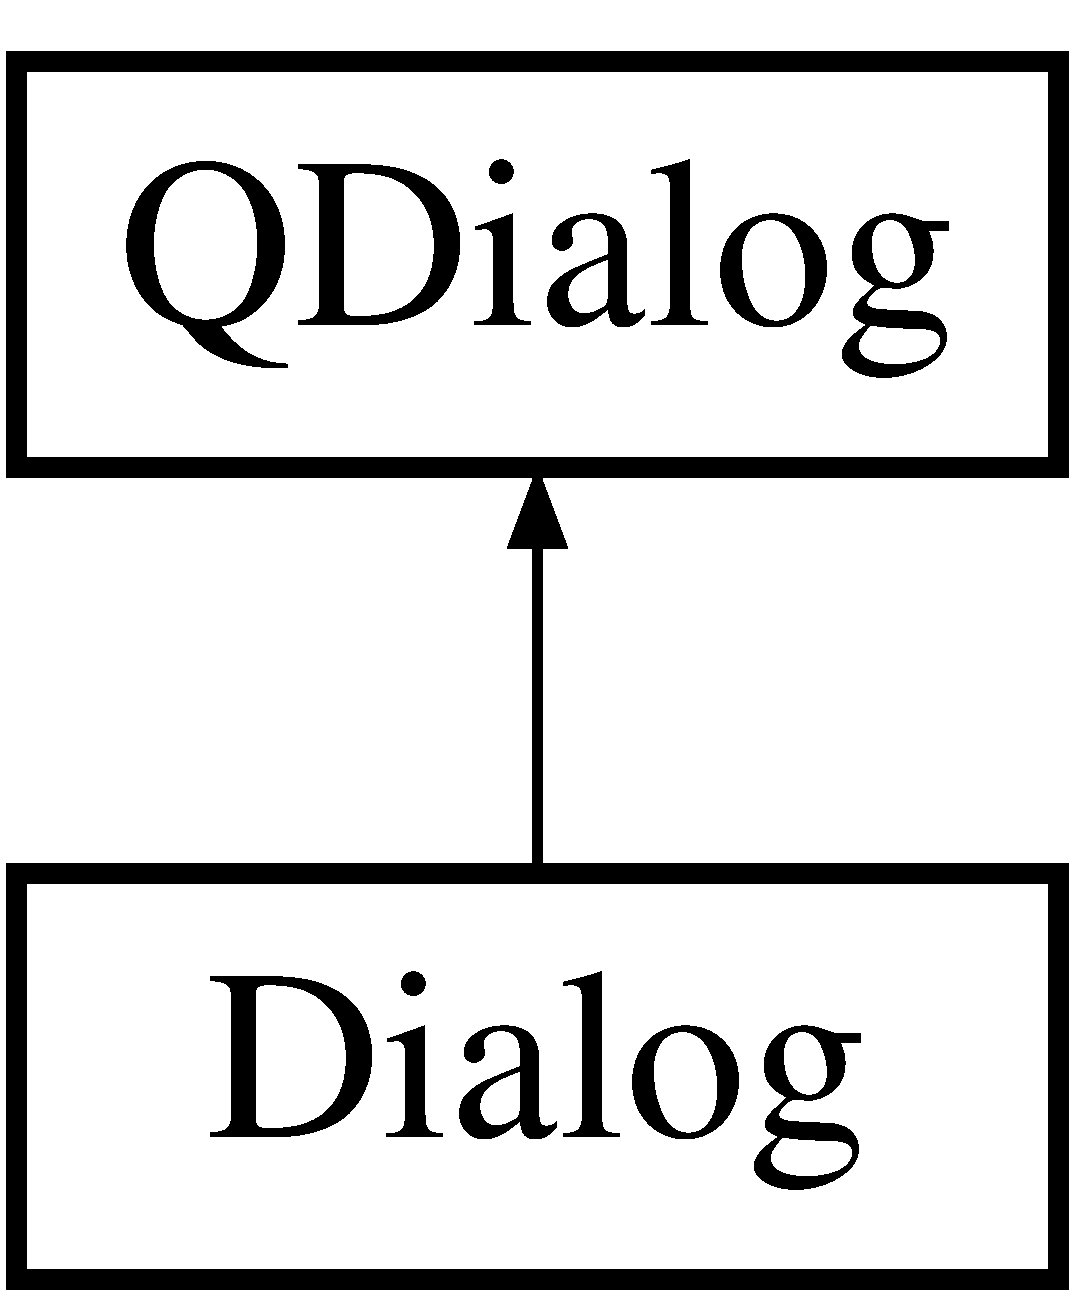
\includegraphics[height=2.000000cm]{classDialog}
\end{center}
\end{figure}
\subsection*{Sygnały}
\begin{DoxyCompactItemize}
\item 
void \hyperlink{classDialog_a88d467b80921a394962d27edb36180f6}{connect\-To\-Server} (Q\-String, int)
\end{DoxyCompactItemize}
\subsection*{Metody publiczne}
\begin{DoxyCompactItemize}
\item 
\hyperlink{classDialog_acfa2063f9f962d394c6a645b6e7e08d8}{Dialog} (Q\-Widget $\ast$parent=0)
\item 
\hyperlink{classDialog_a2a1fe6ef28513eed13bfcd3a4da83ccb}{$\sim$\-Dialog} ()
\item 
void \hyperlink{classDialog_ab2375beb017973ea416f1c3f3494c100}{ustaw\-Wiadomosc} (Q\-String)
\begin{DoxyCompactList}\small\item\em ustaw\-Wiadomosc \end{DoxyCompactList}\end{DoxyCompactItemize}
\subsection*{Sloty prywatne}
\begin{DoxyCompactItemize}
\item 
void \hyperlink{classDialog_ae3619019db8ba37af8a2b30491272a28}{on\-\_\-push\-Button\-Polacz\-\_\-clicked} ()
\end{DoxyCompactItemize}
\subsection*{Atrybuty prywatne}
\begin{DoxyCompactItemize}
\item 
\hyperlink{classUi_1_1Dialog}{Ui\-::\-Dialog} $\ast$ \hyperlink{classDialog_aaa4b5bfb9a0f64900d524f14bc32e6df}{ui}
\end{DoxyCompactItemize}


\subsection{Opis szczegółowy}
Okno Dialogowe. 

Umożliwia połączenie z serwerem 

\subsection{Dokumentacja konstruktora i destruktora}
\hypertarget{classDialog_acfa2063f9f962d394c6a645b6e7e08d8}{\index{Dialog@{Dialog}!Dialog@{Dialog}}
\index{Dialog@{Dialog}!Dialog@{Dialog}}
\subsubsection[{Dialog}]{\setlength{\rightskip}{0pt plus 5cm}Dialog\-::\-Dialog (
\begin{DoxyParamCaption}
\item[{Q\-Widget $\ast$}]{parent = {\ttfamily 0}}
\end{DoxyParamCaption}
)\hspace{0.3cm}{\ttfamily [explicit]}}}\label{classDialog_acfa2063f9f962d394c6a645b6e7e08d8}
\hypertarget{classDialog_a2a1fe6ef28513eed13bfcd3a4da83ccb}{\index{Dialog@{Dialog}!$\sim$\-Dialog@{$\sim$\-Dialog}}
\index{$\sim$\-Dialog@{$\sim$\-Dialog}!Dialog@{Dialog}}
\subsubsection[{$\sim$\-Dialog}]{\setlength{\rightskip}{0pt plus 5cm}Dialog\-::$\sim$\-Dialog (
\begin{DoxyParamCaption}
{}
\end{DoxyParamCaption}
)}}\label{classDialog_a2a1fe6ef28513eed13bfcd3a4da83ccb}


\subsection{Dokumentacja funkcji składowych}
\hypertarget{classDialog_a88d467b80921a394962d27edb36180f6}{\index{Dialog@{Dialog}!connect\-To\-Server@{connect\-To\-Server}}
\index{connect\-To\-Server@{connect\-To\-Server}!Dialog@{Dialog}}
\subsubsection[{connect\-To\-Server}]{\setlength{\rightskip}{0pt plus 5cm}void Dialog\-::connect\-To\-Server (
\begin{DoxyParamCaption}
\item[{Q\-String}]{\-\_\-t1, }
\item[{int}]{\-\_\-t2}
\end{DoxyParamCaption}
)\hspace{0.3cm}{\ttfamily [signal]}}}\label{classDialog_a88d467b80921a394962d27edb36180f6}
\hypertarget{classDialog_ae3619019db8ba37af8a2b30491272a28}{\index{Dialog@{Dialog}!on\-\_\-push\-Button\-Polacz\-\_\-clicked@{on\-\_\-push\-Button\-Polacz\-\_\-clicked}}
\index{on\-\_\-push\-Button\-Polacz\-\_\-clicked@{on\-\_\-push\-Button\-Polacz\-\_\-clicked}!Dialog@{Dialog}}
\subsubsection[{on\-\_\-push\-Button\-Polacz\-\_\-clicked}]{\setlength{\rightskip}{0pt plus 5cm}void Dialog\-::on\-\_\-push\-Button\-Polacz\-\_\-clicked (
\begin{DoxyParamCaption}
{}
\end{DoxyParamCaption}
)\hspace{0.3cm}{\ttfamily [private]}, {\ttfamily [slot]}}}\label{classDialog_ae3619019db8ba37af8a2b30491272a28}
Służy do połączenia klienta z serwerem \hypertarget{classDialog_ab2375beb017973ea416f1c3f3494c100}{\index{Dialog@{Dialog}!ustaw\-Wiadomosc@{ustaw\-Wiadomosc}}
\index{ustaw\-Wiadomosc@{ustaw\-Wiadomosc}!Dialog@{Dialog}}
\subsubsection[{ustaw\-Wiadomosc}]{\setlength{\rightskip}{0pt plus 5cm}void Dialog\-::ustaw\-Wiadomosc (
\begin{DoxyParamCaption}
\item[{Q\-String}]{wiadomosc}
\end{DoxyParamCaption}
)}}\label{classDialog_ab2375beb017973ea416f1c3f3494c100}


ustaw\-Wiadomosc 

Ustawia wiadomość w oknie dialogowym 

\subsection{Dokumentacja atrybutów składowych}
\hypertarget{classDialog_aaa4b5bfb9a0f64900d524f14bc32e6df}{\index{Dialog@{Dialog}!ui@{ui}}
\index{ui@{ui}!Dialog@{Dialog}}
\subsubsection[{ui}]{\setlength{\rightskip}{0pt plus 5cm}{\bf Ui\-::\-Dialog}$\ast$ Dialog\-::ui\hspace{0.3cm}{\ttfamily [private]}}}\label{classDialog_aaa4b5bfb9a0f64900d524f14bc32e6df}


Dokumentacja dla tej klasy została wygenerowana z plików\-:\begin{DoxyCompactItemize}
\item 
Gra\-Figury/\hyperlink{dialog_8h}{dialog.\-h}\item 
Gra\-Figury/\hyperlink{dialog_8cpp}{dialog.\-cpp}\item 
Gra\-Figury/\hyperlink{moc__dialog_8cpp}{moc\-\_\-dialog.\-cpp}\end{DoxyCompactItemize}

\hypertarget{classUi_1_1Dialog}{\section{Dokumentacja klasy Ui\-:\-:Dialog}
\label{classUi_1_1Dialog}\index{Ui\-::\-Dialog@{Ui\-::\-Dialog}}
}


{\ttfamily \#include $<$ui\-\_\-dialog.\-h$>$}

Diagram dziedziczenia dla Ui\-:\-:Dialog\begin{figure}[H]
\begin{center}
\leavevmode
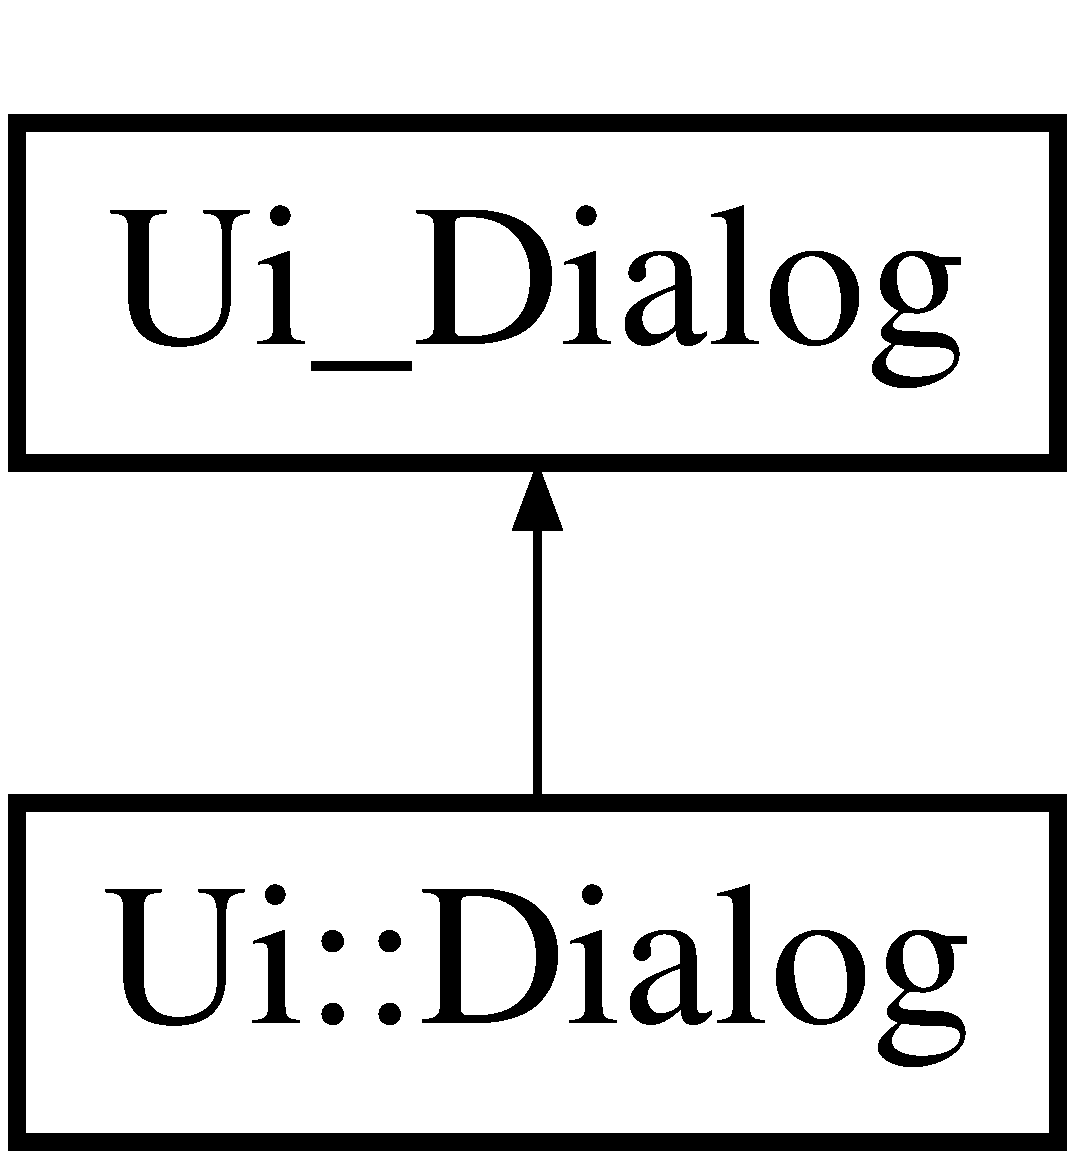
\includegraphics[height=2.000000cm]{classUi_1_1Dialog}
\end{center}
\end{figure}
\subsection*{Dodatkowe Dziedziczone Składowe}


Dokumentacja dla tej klasy została wygenerowana z pliku\-:\begin{DoxyCompactItemize}
\item 
Gra\-Figury/\hyperlink{ui__dialog_8h}{ui\-\_\-dialog.\-h}\end{DoxyCompactItemize}

\hypertarget{classDialog2}{\section{Dokumentacja klasy Dialog2}
\label{classDialog2}\index{Dialog2@{Dialog2}}
}


Okno Dialogowe.  




{\ttfamily \#include $<$dialog2.\-h$>$}

Diagram dziedziczenia dla Dialog2\begin{figure}[H]
\begin{center}
\leavevmode
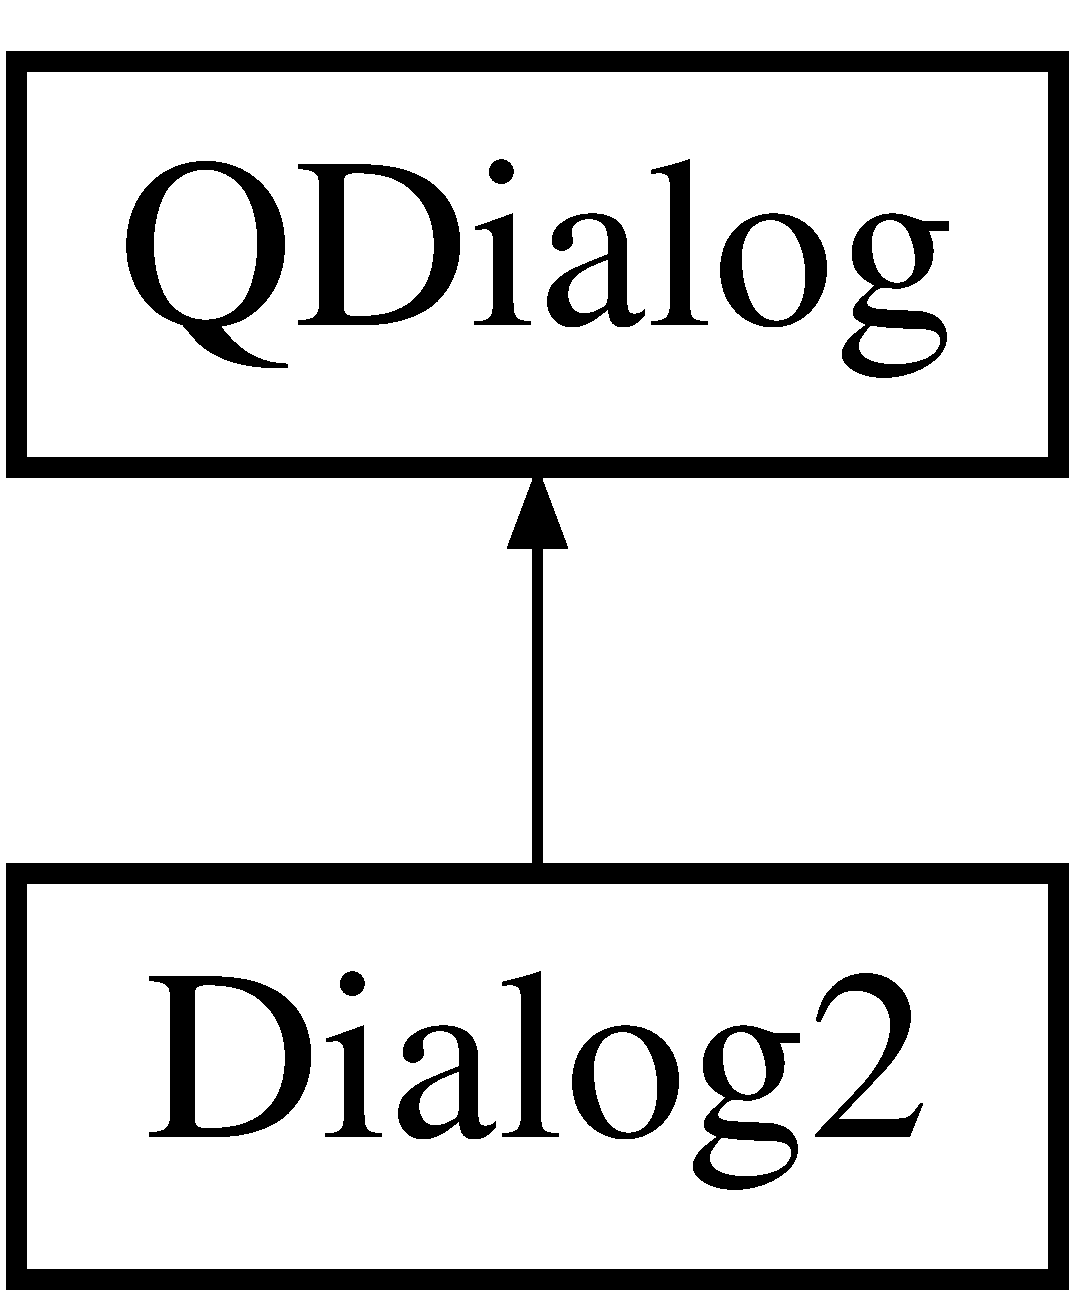
\includegraphics[height=2.000000cm]{classDialog2}
\end{center}
\end{figure}
\subsection*{Sygnały}
\begin{DoxyCompactItemize}
\item 
void \hyperlink{classDialog2_a05e8df578a22d2428319b06f65512fd4}{zmien\-Poziom} ()
\end{DoxyCompactItemize}
\subsection*{Metody publiczne}
\begin{DoxyCompactItemize}
\item 
\hyperlink{classDialog2_a78ae31daad000669cd54a31271ce9470}{Dialog2} (Q\-Widget $\ast$parent=0)
\item 
\hyperlink{classDialog2_ae4ceaef72d01b76dcd126b54c875dfaa}{$\sim$\-Dialog2} ()
\item 
void \hyperlink{classDialog2_a7c9262df7b7ea4f6250abdb0f6612a5f}{ustaw\-Wiadomosc} (Q\-String)
\begin{DoxyCompactList}\small\item\em \hyperlink{classDialog2_a7c9262df7b7ea4f6250abdb0f6612a5f}{Dialog2\-::ustaw\-Wiadomosc}. \end{DoxyCompactList}\end{DoxyCompactItemize}
\subsection*{Sloty prywatne}
\begin{DoxyCompactItemize}
\item 
void \hyperlink{classDialog2_a50271de9b195c7b846e00c1f789ddf4e}{on\-\_\-push\-Button\-\_\-2\-\_\-clicked} ()
\end{DoxyCompactItemize}
\subsection*{Atrybuty prywatne}
\begin{DoxyCompactItemize}
\item 
\hyperlink{classUi_1_1Dialog2}{Ui\-::\-Dialog2} $\ast$ \hyperlink{classDialog2_a321aadfcfc152fc97dc63391f08216fa}{ui}
\end{DoxyCompactItemize}


\subsection{Opis szczegółowy}
Okno Dialogowe. 

Wyświetlane po ukończeniu poziomu 

\subsection{Dokumentacja konstruktora i destruktora}
\hypertarget{classDialog2_a78ae31daad000669cd54a31271ce9470}{\index{Dialog2@{Dialog2}!Dialog2@{Dialog2}}
\index{Dialog2@{Dialog2}!Dialog2@{Dialog2}}
\subsubsection[{Dialog2}]{\setlength{\rightskip}{0pt plus 5cm}Dialog2\-::\-Dialog2 (
\begin{DoxyParamCaption}
\item[{Q\-Widget $\ast$}]{parent = {\ttfamily 0}}
\end{DoxyParamCaption}
)\hspace{0.3cm}{\ttfamily [explicit]}}}\label{classDialog2_a78ae31daad000669cd54a31271ce9470}
\hypertarget{classDialog2_ae4ceaef72d01b76dcd126b54c875dfaa}{\index{Dialog2@{Dialog2}!$\sim$\-Dialog2@{$\sim$\-Dialog2}}
\index{$\sim$\-Dialog2@{$\sim$\-Dialog2}!Dialog2@{Dialog2}}
\subsubsection[{$\sim$\-Dialog2}]{\setlength{\rightskip}{0pt plus 5cm}Dialog2\-::$\sim$\-Dialog2 (
\begin{DoxyParamCaption}
{}
\end{DoxyParamCaption}
)}}\label{classDialog2_ae4ceaef72d01b76dcd126b54c875dfaa}


\subsection{Dokumentacja funkcji składowych}
\hypertarget{classDialog2_a50271de9b195c7b846e00c1f789ddf4e}{\index{Dialog2@{Dialog2}!on\-\_\-push\-Button\-\_\-2\-\_\-clicked@{on\-\_\-push\-Button\-\_\-2\-\_\-clicked}}
\index{on\-\_\-push\-Button\-\_\-2\-\_\-clicked@{on\-\_\-push\-Button\-\_\-2\-\_\-clicked}!Dialog2@{Dialog2}}
\subsubsection[{on\-\_\-push\-Button\-\_\-2\-\_\-clicked}]{\setlength{\rightskip}{0pt plus 5cm}void Dialog2\-::on\-\_\-push\-Button\-\_\-2\-\_\-clicked (
\begin{DoxyParamCaption}
{}
\end{DoxyParamCaption}
)\hspace{0.3cm}{\ttfamily [private]}, {\ttfamily [slot]}}}\label{classDialog2_a50271de9b195c7b846e00c1f789ddf4e}
Po wciśnięciu przycisku zostanie przesłana informacja o zmianie poziomu \hypertarget{classDialog2_a7c9262df7b7ea4f6250abdb0f6612a5f}{\index{Dialog2@{Dialog2}!ustaw\-Wiadomosc@{ustaw\-Wiadomosc}}
\index{ustaw\-Wiadomosc@{ustaw\-Wiadomosc}!Dialog2@{Dialog2}}
\subsubsection[{ustaw\-Wiadomosc}]{\setlength{\rightskip}{0pt plus 5cm}void Dialog2\-::ustaw\-Wiadomosc (
\begin{DoxyParamCaption}
\item[{Q\-String}]{wiadomosc}
\end{DoxyParamCaption}
)}}\label{classDialog2_a7c9262df7b7ea4f6250abdb0f6612a5f}


\hyperlink{classDialog2_a7c9262df7b7ea4f6250abdb0f6612a5f}{Dialog2\-::ustaw\-Wiadomosc}. 


\begin{DoxyParams}{Parametry}
{\em wiadomosc} & Ustawia wiadomość w oknie dialogowym \\
\hline
\end{DoxyParams}
\hypertarget{classDialog2_a05e8df578a22d2428319b06f65512fd4}{\index{Dialog2@{Dialog2}!zmien\-Poziom@{zmien\-Poziom}}
\index{zmien\-Poziom@{zmien\-Poziom}!Dialog2@{Dialog2}}
\subsubsection[{zmien\-Poziom}]{\setlength{\rightskip}{0pt plus 5cm}void Dialog2\-::zmien\-Poziom (
\begin{DoxyParamCaption}
{}
\end{DoxyParamCaption}
)\hspace{0.3cm}{\ttfamily [signal]}}}\label{classDialog2_a05e8df578a22d2428319b06f65512fd4}


\subsection{Dokumentacja atrybutów składowych}
\hypertarget{classDialog2_a321aadfcfc152fc97dc63391f08216fa}{\index{Dialog2@{Dialog2}!ui@{ui}}
\index{ui@{ui}!Dialog2@{Dialog2}}
\subsubsection[{ui}]{\setlength{\rightskip}{0pt plus 5cm}{\bf Ui\-::\-Dialog2}$\ast$ Dialog2\-::ui\hspace{0.3cm}{\ttfamily [private]}}}\label{classDialog2_a321aadfcfc152fc97dc63391f08216fa}


Dokumentacja dla tej klasy została wygenerowana z plików\-:\begin{DoxyCompactItemize}
\item 
Gra\-Figury/\hyperlink{dialog2_8h}{dialog2.\-h}\item 
Gra\-Figury/\hyperlink{dialog2_8cpp}{dialog2.\-cpp}\item 
Gra\-Figury/\hyperlink{moc__dialog2_8cpp}{moc\-\_\-dialog2.\-cpp}\end{DoxyCompactItemize}

\hypertarget{classUi_1_1Dialog2}{\section{Dokumentacja klasy Ui\-:\-:Dialog2}
\label{classUi_1_1Dialog2}\index{Ui\-::\-Dialog2@{Ui\-::\-Dialog2}}
}


{\ttfamily \#include $<$ui\-\_\-dialog2.\-h$>$}

Diagram dziedziczenia dla Ui\-:\-:Dialog2\begin{figure}[H]
\begin{center}
\leavevmode
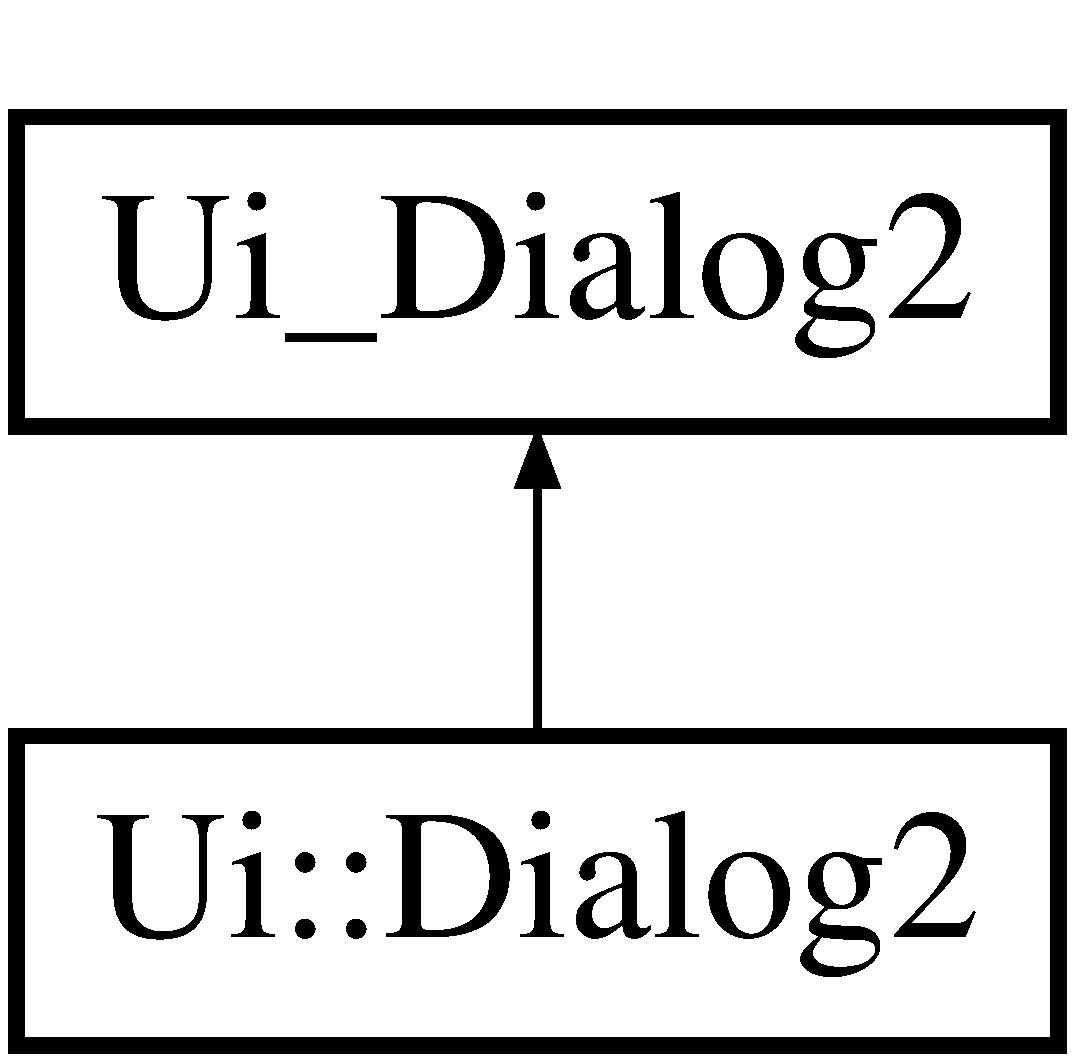
\includegraphics[height=2.000000cm]{classUi_1_1Dialog2}
\end{center}
\end{figure}
\subsection*{Dodatkowe Dziedziczone Składowe}


Dokumentacja dla tej klasy została wygenerowana z pliku\-:\begin{DoxyCompactItemize}
\item 
Gra\-Figury/\hyperlink{ui__dialog2_8h}{ui\-\_\-dialog2.\-h}\end{DoxyCompactItemize}

\hypertarget{classFigura}{\section{Dokumentacja klasy Figura}
\label{classFigura}\index{Figura@{Figura}}
}


The \hyperlink{classFigura}{Figura} class.  




{\ttfamily \#include $<$figura.\-h$>$}

Diagram dziedziczenia dla Figura\begin{figure}[H]
\begin{center}
\leavevmode
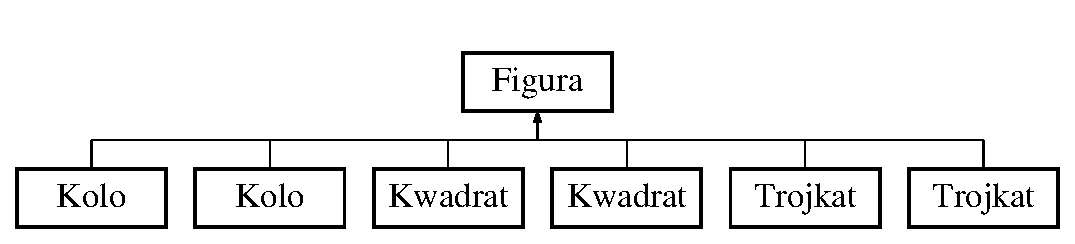
\includegraphics[height=2.000000cm]{classFigura}
\end{center}
\end{figure}
\subsection*{Typy publiczne}
\begin{DoxyCompactItemize}
\item 
enum \{ \\*
\hyperlink{classFigura_aa2d4be66eee786b08617f14e5c1786d6a4437d7afd63785b800b0f3260b12fb02}{K\-O\-L\-O}, 
\hyperlink{classFigura_aa2d4be66eee786b08617f14e5c1786d6abb9c7c24fdf57ec1105b935409abc923}{K\-W\-A\-D\-R\-A\-T}, 
\hyperlink{classFigura_aa2d4be66eee786b08617f14e5c1786d6ab441025a17c84164b9463ba26d33862f}{T\-R\-O\-J\-K\-A\-T}, 
\hyperlink{classFigura_aa2d4be66eee786b08617f14e5c1786d6aca5f505db3a8ad71c5ba3c5522f7850d}{K\-O\-L\-O\-\_\-\-K\-W\-A\-D\-R\-A\-T}, 
\\*
\hyperlink{classFigura_aa2d4be66eee786b08617f14e5c1786d6a83c12346d3bb84606b92ec06a12de9df}{K\-O\-L\-O\-\_\-\-T\-R\-O\-J\-K\-A\-T}, 
\hyperlink{classFigura_aa2d4be66eee786b08617f14e5c1786d6a9099cc2a327bd9fa23fea4966fd6bcd3}{K\-W\-A\-D\-R\-A\-T\-\_\-\-T\-R\-O\-J\-K\-A\-T}, 
\hyperlink{classFigura_aa2d4be66eee786b08617f14e5c1786d6a52f5d0a124a5ba9039a864a13ab58d7e}{K\-W\-A\-D\-R\-A\-T\-\_\-\-K\-O\-L\-O}, 
\hyperlink{classFigura_aa2d4be66eee786b08617f14e5c1786d6a353557c9cac53f4457e0be3bf4c623f5}{T\-R\-O\-J\-K\-A\-T\-\_\-\-K\-O\-L\-O}, 
\\*
\hyperlink{classFigura_aa2d4be66eee786b08617f14e5c1786d6a047ddb0ae4de2865df86a8cbcea0fb9f}{T\-R\-O\-J\-K\-A\-T\-\_\-\-K\-W\-A\-D\-R\-A\-T}
 \}
\item 
enum \{ \\*
\hyperlink{classFigura_aa2d4be66eee786b08617f14e5c1786d6a4437d7afd63785b800b0f3260b12fb02}{K\-O\-L\-O}, 
\hyperlink{classFigura_aa2d4be66eee786b08617f14e5c1786d6abb9c7c24fdf57ec1105b935409abc923}{K\-W\-A\-D\-R\-A\-T}, 
\hyperlink{classFigura_aa2d4be66eee786b08617f14e5c1786d6ab441025a17c84164b9463ba26d33862f}{T\-R\-O\-J\-K\-A\-T}, 
\hyperlink{classFigura_aa2d4be66eee786b08617f14e5c1786d6aca5f505db3a8ad71c5ba3c5522f7850d}{K\-O\-L\-O\-\_\-\-K\-W\-A\-D\-R\-A\-T}, 
\\*
\hyperlink{classFigura_aa2d4be66eee786b08617f14e5c1786d6a83c12346d3bb84606b92ec06a12de9df}{K\-O\-L\-O\-\_\-\-T\-R\-O\-J\-K\-A\-T}, 
\hyperlink{classFigura_aa2d4be66eee786b08617f14e5c1786d6a9099cc2a327bd9fa23fea4966fd6bcd3}{K\-W\-A\-D\-R\-A\-T\-\_\-\-T\-R\-O\-J\-K\-A\-T}, 
\hyperlink{classFigura_aa2d4be66eee786b08617f14e5c1786d6a52f5d0a124a5ba9039a864a13ab58d7e}{K\-W\-A\-D\-R\-A\-T\-\_\-\-K\-O\-L\-O}, 
\hyperlink{classFigura_aa2d4be66eee786b08617f14e5c1786d6a353557c9cac53f4457e0be3bf4c623f5}{T\-R\-O\-J\-K\-A\-T\-\_\-\-K\-O\-L\-O}, 
\\*
\hyperlink{classFigura_aa2d4be66eee786b08617f14e5c1786d6a047ddb0ae4de2865df86a8cbcea0fb9f}{T\-R\-O\-J\-K\-A\-T\-\_\-\-K\-W\-A\-D\-R\-A\-T}
 \}
\end{DoxyCompactItemize}
\subsection*{Metody publiczne}
\begin{DoxyCompactItemize}
\item 
\hyperlink{classFigura_a6977c7f0438c11b985a9a74c208b51c8}{Figura} ()
\begin{DoxyCompactList}\small\item\em Konstruktor domyślny. \end{DoxyCompactList}\item 
\hyperlink{classFigura_a9597f3d418eda29436184422e6347518}{Figura} (float x\-\_\-, float y\-\_\-)
\item 
virtual \hyperlink{classFigura_a6130eb548893c36efcb7933e2da6821e}{$\sim$\-Figura} ()
\item 
float \hyperlink{classFigura_a8221a03216b76b37e11a7e258b2e6b1f}{odleglosc} ()
\item 
float \hyperlink{classFigura_a351dd41d348f9a2adaed7802c12722df}{odleglosc} (\hyperlink{classFigura}{Figura} $\ast$druga)
\item 
float \hyperlink{classFigura_a1b60d6f4763b92efa9cb4307aecea892}{odleglosc} (float, float)
\item 
void \hyperlink{classFigura_a08bbbedf4e27f5f17ba897ea6b1bf7a5}{ustaw\-Kolor} (float red, float green, float blue, float \hyperlink{classFigura_a601361fbb05bc4dc3b9cab1a868b2910}{alpha})
\item 
void \hyperlink{classFigura_a6e7a5f23810da2aa73f2ad28f8918d31}{ustaw\-Predkosc\-X} (float vx)
\item 
void \hyperlink{classFigura_a22ffec44b60184584f94e1fcd95bf5b5}{ustaw\-Predkosc\-Y} (float vy)
\item 
void \hyperlink{classFigura_a93bd750b3c4311f584fe2e1d899b470a}{ustaw\-Omega} (float v)
\item 
float \hyperlink{classFigura_a33b849c7f3a12e260ae6294f1120b4bd}{zwroc\-Predkosc\-X} ()
\item 
float \hyperlink{classFigura_a6d40d8f173b099d9e76d7a7ccc73a0cb}{zwroc\-Predkosc\-Y} ()
\item 
float \hyperlink{classFigura_a94da9ef8eb433270570abd5074dbd3fa}{zwroc\-Omega} ()
\item 
void \hyperlink{classFigura_a8eaf7fc68e05ce5a602ae741759e36e4}{zmien\-Polozenie} (float dx, float dy)
\item 
void \hyperlink{classFigura_ab017b5da886407a1a809f15ed9ab32f4}{zmien\-Alpha} (float da)
\item 
float \hyperlink{classFigura_a009283dfbe0ed4e538c6fc857c544f29}{zwroc\-Polozenie\-X} ()
\item 
float \hyperlink{classFigura_aba4eb260f9d5f7ff7a52e9eb8fc99f5c}{zwroc\-Polozenie\-Y} ()
\item 
float \hyperlink{classFigura_a3cfd45edd89e226a1fb44d8f4d3f7a56}{zwroc\-Alpha} ()
\item 
void \hyperlink{classFigura_aef7fbdf672096d76336a460bcfb3108a}{ustaw\-Specjalnym} (int)
\item 
void \hyperlink{classFigura_ac5df5b70874e675dc1463b8ddc68612b}{ustaw\-Rozmiar} (float)
\item 
virtual void \hyperlink{classFigura_a6ec035fbeb95129af6ca64d2adff7651}{rysuj} ()=0
\item 
virtual bool \hyperlink{classFigura_a14f9ba21828b6292488e1fa12bf1b85f}{czy\-Nalezydo\-Figury} (float \hyperlink{classFigura_ad640a05ebb1ddbf595124f0b31793e8a}{x}, float \hyperlink{classFigura_ab17e5953f2898eb729b2dc506640bce2}{y})=0
\item 
virtual float \hyperlink{classFigura_aaeb587028aafd028e134079c249b0c88}{zwroc\-Rozmiar} ()=0
\item 
virtual bool \hyperlink{classFigura_a7a1cb0014aaaa276f8b17932c394b485}{czy\-Kolizja} (\hyperlink{classFigura}{Figura} $\ast$druga)=0
\item 
virtual double \hyperlink{classFigura_a3e534b43a279aeec36c5b28ac731e0f8}{zwrocodleglosc\-Do\-Kolizji} ()=0
\item 
virtual void \hyperlink{classFigura_a7ea2c8b450129878f4347404b8834c6b}{zmien\-Rozmiar} (float)=0
\item 
virtual float \hyperlink{classFigura_a78861f3fce7e615ba30b47aa1cdcebec}{zwroc\-Pole} ()=0
\item 
virtual void \hyperlink{classFigura_aad1198cc826aa6b3036454fd4f3bb5b3}{zmien\-Pole} (float)=0
\item 
virtual int \hyperlink{classFigura_ab04732de63f17d4c3776990d24897db7}{zwroc\-Typ} ()=0
\item 
\hyperlink{classFigura_a6977c7f0438c11b985a9a74c208b51c8}{Figura} ()
\item 
\hyperlink{classFigura_a9597f3d418eda29436184422e6347518}{Figura} (float x\-\_\-, float y\-\_\-)
\item 
virtual \hyperlink{classFigura_a80761a9b9f258fac7c22c3dd5ebf5820}{$\sim$\-Figura} ()
\item 
float \hyperlink{classFigura_a8221a03216b76b37e11a7e258b2e6b1f}{odleglosc} ()
\item 
float \hyperlink{classFigura_a351dd41d348f9a2adaed7802c12722df}{odleglosc} (\hyperlink{classFigura}{Figura} $\ast$druga)
\item 
float \hyperlink{classFigura_a1b60d6f4763b92efa9cb4307aecea892}{odleglosc} (float, float)
\item 
void \hyperlink{classFigura_a08bbbedf4e27f5f17ba897ea6b1bf7a5}{ustaw\-Kolor} (float red, float green, float blue, float \hyperlink{classFigura_a601361fbb05bc4dc3b9cab1a868b2910}{alpha})
\item 
void \hyperlink{classFigura_a6e7a5f23810da2aa73f2ad28f8918d31}{ustaw\-Predkosc\-X} (float vx)
\item 
void \hyperlink{classFigura_a22ffec44b60184584f94e1fcd95bf5b5}{ustaw\-Predkosc\-Y} (float vy)
\item 
void \hyperlink{classFigura_a93bd750b3c4311f584fe2e1d899b470a}{ustaw\-Omega} (float v)
\item 
float \hyperlink{classFigura_a33b849c7f3a12e260ae6294f1120b4bd}{zwroc\-Predkosc\-X} ()
\item 
float \hyperlink{classFigura_a6d40d8f173b099d9e76d7a7ccc73a0cb}{zwroc\-Predkosc\-Y} ()
\item 
float \hyperlink{classFigura_a94da9ef8eb433270570abd5074dbd3fa}{zwroc\-Omega} ()
\item 
void \hyperlink{classFigura_a8eaf7fc68e05ce5a602ae741759e36e4}{zmien\-Polozenie} (float dx, float dy)
\item 
void \hyperlink{classFigura_ab017b5da886407a1a809f15ed9ab32f4}{zmien\-Alpha} (float da)
\item 
float \hyperlink{classFigura_a009283dfbe0ed4e538c6fc857c544f29}{zwroc\-Polozenie\-X} ()
\item 
float \hyperlink{classFigura_aba4eb260f9d5f7ff7a52e9eb8fc99f5c}{zwroc\-Polozenie\-Y} ()
\item 
float \hyperlink{classFigura_a3cfd45edd89e226a1fb44d8f4d3f7a56}{zwroc\-Alpha} ()
\item 
void \hyperlink{classFigura_aef7fbdf672096d76336a460bcfb3108a}{ustaw\-Specjalnym} (int)
\item 
void \hyperlink{classFigura_ac5df5b70874e675dc1463b8ddc68612b}{ustaw\-Rozmiar} (float)
\item 
virtual void \hyperlink{classFigura_a6ec035fbeb95129af6ca64d2adff7651}{rysuj} ()=0
\item 
virtual bool \hyperlink{classFigura_a14f9ba21828b6292488e1fa12bf1b85f}{czy\-Nalezydo\-Figury} (float \hyperlink{classFigura_ad640a05ebb1ddbf595124f0b31793e8a}{x}, float \hyperlink{classFigura_ab17e5953f2898eb729b2dc506640bce2}{y})=0
\item 
virtual float \hyperlink{classFigura_aaeb587028aafd028e134079c249b0c88}{zwroc\-Rozmiar} ()=0
\item 
virtual bool \hyperlink{classFigura_a7a1cb0014aaaa276f8b17932c394b485}{czy\-Kolizja} (\hyperlink{classFigura}{Figura} $\ast$druga)=0
\item 
virtual double \hyperlink{classFigura_a3e534b43a279aeec36c5b28ac731e0f8}{zwrocodleglosc\-Do\-Kolizji} ()=0
\item 
virtual void \hyperlink{classFigura_a7ea2c8b450129878f4347404b8834c6b}{zmien\-Rozmiar} (float)=0
\item 
virtual float \hyperlink{classFigura_a78861f3fce7e615ba30b47aa1cdcebec}{zwroc\-Pole} ()=0
\item 
virtual void \hyperlink{classFigura_aad1198cc826aa6b3036454fd4f3bb5b3}{zmien\-Pole} (float)=0
\item 
virtual int \hyperlink{classFigura_ab04732de63f17d4c3776990d24897db7}{zwroc\-Typ} ()=0
\end{DoxyCompactItemize}
\subsection*{Atrybuty chronione}
\begin{DoxyCompactItemize}
\item 
float \hyperlink{classFigura_ad640a05ebb1ddbf595124f0b31793e8a}{x}
\item 
float \hyperlink{classFigura_ab17e5953f2898eb729b2dc506640bce2}{y}
\item 
float \hyperlink{classFigura_af4ea0a1b316060276b8cde2bc11ca190}{r}
\item 
float \hyperlink{classFigura_ab05a5e9bebed67a5d20d758999cd5d1a}{kolor} \mbox{[}4\mbox{]}
\item 
float \hyperlink{classFigura_a890207e032e201a3a75ab9680c90dec7}{predkosc} \mbox{[}2\mbox{]}
\item 
float \hyperlink{classFigura_a01436a48e3702376968890266d045dbe}{omega}
\item 
float \hyperlink{classFigura_a601361fbb05bc4dc3b9cab1a868b2910}{alpha}
\item 
int \hyperlink{classFigura_aa722cfdbd1f53bda5f8e8ad5bc7b824d}{typ}
\item 
int \hyperlink{classFigura_a4f37ab8e74deceecf994b1451413e482}{specjalny}
\end{DoxyCompactItemize}
\subsection*{Przyjaciele}
\begin{DoxyCompactItemize}
\item 
Q\-Data\-Stream \& \hyperlink{classFigura_ae62458d63e738dc0b2f191aff1693469}{operator$<$$<$} (Q\-Data\-Stream \&stream, \hyperlink{classFigura}{Figura} $\ast$figura)
\item 
Q\-Data\-Stream \& \hyperlink{classFigura_ab48c431f34046c3a42ab680f39a4b74d}{operator$>$$>$} (Q\-Data\-Stream \&stream, \hyperlink{classFigura}{Figura} $\ast$figura)
\item 
Q\-Data\-Stream \& \hyperlink{classFigura_aae3d696b5c2d831dd978688411e31163}{operator$<$$<$} (Q\-Data\-Stream \&stream, Q\-List$<$ \hyperlink{classFigura}{Figura} $\ast$ $>$ \&lista\-Figur)
\item 
Q\-Data\-Stream \& \hyperlink{classFigura_a1e4d4e9a4c99027be2b103f5bc9ad212}{operator$>$$>$} (Q\-Data\-Stream \&stream, Q\-List$<$ \hyperlink{classFigura}{Figura} $\ast$ $>$ \&lista\-Figur)
\item 
Q\-Data\-Stream \& \hyperlink{classFigura_ae62458d63e738dc0b2f191aff1693469}{operator$<$$<$} (Q\-Data\-Stream \&stream, \hyperlink{classFigura}{Figura} $\ast$figura)
\item 
Q\-Data\-Stream \& \hyperlink{classFigura_ab48c431f34046c3a42ab680f39a4b74d}{operator$>$$>$} (Q\-Data\-Stream \&stream, \hyperlink{classFigura}{Figura} $\ast$figura)
\item 
Q\-Data\-Stream \& \hyperlink{classFigura_aae3d696b5c2d831dd978688411e31163}{operator$<$$<$} (Q\-Data\-Stream \&stream, Q\-List$<$ \hyperlink{classFigura}{Figura} $\ast$ $>$ \&lista\-Figur)
\item 
Q\-Data\-Stream \& \hyperlink{classFigura_a1e4d4e9a4c99027be2b103f5bc9ad212}{operator$>$$>$} (Q\-Data\-Stream \&stream, Q\-List$<$ \hyperlink{classFigura}{Figura} $\ast$ $>$ \&lista\-Figur)
\end{DoxyCompactItemize}


\subsection{Opis szczegółowy}
The \hyperlink{classFigura}{Figura} class. 

Klasa bazowa dla klasy \hyperlink{classKolo}{Kolo}, \hyperlink{classKwadrat}{Kwadrat}, \hyperlink{classTrojkat}{Trojkat} 

\subsection{Dokumentacja składowych wyliczanych}
\hypertarget{classFigura_a6f7cd649a13156167699a95d14e7b94c}{\subsubsection[{anonymous enum}]{\setlength{\rightskip}{0pt plus 5cm}anonymous enum}}\label{classFigura_a6f7cd649a13156167699a95d14e7b94c}
\begin{Desc}
\item[Wartości wyliczeń]\par
\begin{description}
\index{K\-O\-L\-O@{K\-O\-L\-O}!Figura@{Figura}}\index{Figura@{Figura}!K\-O\-L\-O@{K\-O\-L\-O}}\item[{\em 
\hypertarget{classFigura_aa2d4be66eee786b08617f14e5c1786d6a4437d7afd63785b800b0f3260b12fb02}{K\-O\-L\-O}\label{classFigura_aa2d4be66eee786b08617f14e5c1786d6a4437d7afd63785b800b0f3260b12fb02}
}]\index{K\-W\-A\-D\-R\-A\-T@{K\-W\-A\-D\-R\-A\-T}!Figura@{Figura}}\index{Figura@{Figura}!K\-W\-A\-D\-R\-A\-T@{K\-W\-A\-D\-R\-A\-T}}\item[{\em 
\hypertarget{classFigura_aa2d4be66eee786b08617f14e5c1786d6abb9c7c24fdf57ec1105b935409abc923}{K\-W\-A\-D\-R\-A\-T}\label{classFigura_aa2d4be66eee786b08617f14e5c1786d6abb9c7c24fdf57ec1105b935409abc923}
}]\index{T\-R\-O\-J\-K\-A\-T@{T\-R\-O\-J\-K\-A\-T}!Figura@{Figura}}\index{Figura@{Figura}!T\-R\-O\-J\-K\-A\-T@{T\-R\-O\-J\-K\-A\-T}}\item[{\em 
\hypertarget{classFigura_aa2d4be66eee786b08617f14e5c1786d6ab441025a17c84164b9463ba26d33862f}{T\-R\-O\-J\-K\-A\-T}\label{classFigura_aa2d4be66eee786b08617f14e5c1786d6ab441025a17c84164b9463ba26d33862f}
}]\index{K\-O\-L\-O\-\_\-\-K\-W\-A\-D\-R\-A\-T@{K\-O\-L\-O\-\_\-\-K\-W\-A\-D\-R\-A\-T}!Figura@{Figura}}\index{Figura@{Figura}!K\-O\-L\-O\-\_\-\-K\-W\-A\-D\-R\-A\-T@{K\-O\-L\-O\-\_\-\-K\-W\-A\-D\-R\-A\-T}}\item[{\em 
\hypertarget{classFigura_aa2d4be66eee786b08617f14e5c1786d6aca5f505db3a8ad71c5ba3c5522f7850d}{K\-O\-L\-O\-\_\-\-K\-W\-A\-D\-R\-A\-T}\label{classFigura_aa2d4be66eee786b08617f14e5c1786d6aca5f505db3a8ad71c5ba3c5522f7850d}
}]\index{K\-O\-L\-O\-\_\-\-T\-R\-O\-J\-K\-A\-T@{K\-O\-L\-O\-\_\-\-T\-R\-O\-J\-K\-A\-T}!Figura@{Figura}}\index{Figura@{Figura}!K\-O\-L\-O\-\_\-\-T\-R\-O\-J\-K\-A\-T@{K\-O\-L\-O\-\_\-\-T\-R\-O\-J\-K\-A\-T}}\item[{\em 
\hypertarget{classFigura_aa2d4be66eee786b08617f14e5c1786d6a83c12346d3bb84606b92ec06a12de9df}{K\-O\-L\-O\-\_\-\-T\-R\-O\-J\-K\-A\-T}\label{classFigura_aa2d4be66eee786b08617f14e5c1786d6a83c12346d3bb84606b92ec06a12de9df}
}]\index{K\-W\-A\-D\-R\-A\-T\-\_\-\-T\-R\-O\-J\-K\-A\-T@{K\-W\-A\-D\-R\-A\-T\-\_\-\-T\-R\-O\-J\-K\-A\-T}!Figura@{Figura}}\index{Figura@{Figura}!K\-W\-A\-D\-R\-A\-T\-\_\-\-T\-R\-O\-J\-K\-A\-T@{K\-W\-A\-D\-R\-A\-T\-\_\-\-T\-R\-O\-J\-K\-A\-T}}\item[{\em 
\hypertarget{classFigura_aa2d4be66eee786b08617f14e5c1786d6a9099cc2a327bd9fa23fea4966fd6bcd3}{K\-W\-A\-D\-R\-A\-T\-\_\-\-T\-R\-O\-J\-K\-A\-T}\label{classFigura_aa2d4be66eee786b08617f14e5c1786d6a9099cc2a327bd9fa23fea4966fd6bcd3}
}]\index{K\-W\-A\-D\-R\-A\-T\-\_\-\-K\-O\-L\-O@{K\-W\-A\-D\-R\-A\-T\-\_\-\-K\-O\-L\-O}!Figura@{Figura}}\index{Figura@{Figura}!K\-W\-A\-D\-R\-A\-T\-\_\-\-K\-O\-L\-O@{K\-W\-A\-D\-R\-A\-T\-\_\-\-K\-O\-L\-O}}\item[{\em 
\hypertarget{classFigura_aa2d4be66eee786b08617f14e5c1786d6a52f5d0a124a5ba9039a864a13ab58d7e}{K\-W\-A\-D\-R\-A\-T\-\_\-\-K\-O\-L\-O}\label{classFigura_aa2d4be66eee786b08617f14e5c1786d6a52f5d0a124a5ba9039a864a13ab58d7e}
}]\index{T\-R\-O\-J\-K\-A\-T\-\_\-\-K\-O\-L\-O@{T\-R\-O\-J\-K\-A\-T\-\_\-\-K\-O\-L\-O}!Figura@{Figura}}\index{Figura@{Figura}!T\-R\-O\-J\-K\-A\-T\-\_\-\-K\-O\-L\-O@{T\-R\-O\-J\-K\-A\-T\-\_\-\-K\-O\-L\-O}}\item[{\em 
\hypertarget{classFigura_aa2d4be66eee786b08617f14e5c1786d6a353557c9cac53f4457e0be3bf4c623f5}{T\-R\-O\-J\-K\-A\-T\-\_\-\-K\-O\-L\-O}\label{classFigura_aa2d4be66eee786b08617f14e5c1786d6a353557c9cac53f4457e0be3bf4c623f5}
}]\index{T\-R\-O\-J\-K\-A\-T\-\_\-\-K\-W\-A\-D\-R\-A\-T@{T\-R\-O\-J\-K\-A\-T\-\_\-\-K\-W\-A\-D\-R\-A\-T}!Figura@{Figura}}\index{Figura@{Figura}!T\-R\-O\-J\-K\-A\-T\-\_\-\-K\-W\-A\-D\-R\-A\-T@{T\-R\-O\-J\-K\-A\-T\-\_\-\-K\-W\-A\-D\-R\-A\-T}}\item[{\em 
\hypertarget{classFigura_aa2d4be66eee786b08617f14e5c1786d6a047ddb0ae4de2865df86a8cbcea0fb9f}{T\-R\-O\-J\-K\-A\-T\-\_\-\-K\-W\-A\-D\-R\-A\-T}\label{classFigura_aa2d4be66eee786b08617f14e5c1786d6a047ddb0ae4de2865df86a8cbcea0fb9f}
}]\end{description}
\end{Desc}
\hypertarget{classFigura_aa2d4be66eee786b08617f14e5c1786d6}{\subsubsection[{anonymous enum}]{\setlength{\rightskip}{0pt plus 5cm}anonymous enum}}\label{classFigura_aa2d4be66eee786b08617f14e5c1786d6}
\begin{Desc}
\item[Wartości wyliczeń]\par
\begin{description}
\index{K\-O\-L\-O@{K\-O\-L\-O}!Figura@{Figura}}\index{Figura@{Figura}!K\-O\-L\-O@{K\-O\-L\-O}}\item[{\em 
\hypertarget{classFigura_aa2d4be66eee786b08617f14e5c1786d6a4437d7afd63785b800b0f3260b12fb02}{K\-O\-L\-O}\label{classFigura_aa2d4be66eee786b08617f14e5c1786d6a4437d7afd63785b800b0f3260b12fb02}
}]\index{K\-W\-A\-D\-R\-A\-T@{K\-W\-A\-D\-R\-A\-T}!Figura@{Figura}}\index{Figura@{Figura}!K\-W\-A\-D\-R\-A\-T@{K\-W\-A\-D\-R\-A\-T}}\item[{\em 
\hypertarget{classFigura_aa2d4be66eee786b08617f14e5c1786d6abb9c7c24fdf57ec1105b935409abc923}{K\-W\-A\-D\-R\-A\-T}\label{classFigura_aa2d4be66eee786b08617f14e5c1786d6abb9c7c24fdf57ec1105b935409abc923}
}]\index{T\-R\-O\-J\-K\-A\-T@{T\-R\-O\-J\-K\-A\-T}!Figura@{Figura}}\index{Figura@{Figura}!T\-R\-O\-J\-K\-A\-T@{T\-R\-O\-J\-K\-A\-T}}\item[{\em 
\hypertarget{classFigura_aa2d4be66eee786b08617f14e5c1786d6ab441025a17c84164b9463ba26d33862f}{T\-R\-O\-J\-K\-A\-T}\label{classFigura_aa2d4be66eee786b08617f14e5c1786d6ab441025a17c84164b9463ba26d33862f}
}]\index{K\-O\-L\-O\-\_\-\-K\-W\-A\-D\-R\-A\-T@{K\-O\-L\-O\-\_\-\-K\-W\-A\-D\-R\-A\-T}!Figura@{Figura}}\index{Figura@{Figura}!K\-O\-L\-O\-\_\-\-K\-W\-A\-D\-R\-A\-T@{K\-O\-L\-O\-\_\-\-K\-W\-A\-D\-R\-A\-T}}\item[{\em 
\hypertarget{classFigura_aa2d4be66eee786b08617f14e5c1786d6aca5f505db3a8ad71c5ba3c5522f7850d}{K\-O\-L\-O\-\_\-\-K\-W\-A\-D\-R\-A\-T}\label{classFigura_aa2d4be66eee786b08617f14e5c1786d6aca5f505db3a8ad71c5ba3c5522f7850d}
}]\index{K\-O\-L\-O\-\_\-\-T\-R\-O\-J\-K\-A\-T@{K\-O\-L\-O\-\_\-\-T\-R\-O\-J\-K\-A\-T}!Figura@{Figura}}\index{Figura@{Figura}!K\-O\-L\-O\-\_\-\-T\-R\-O\-J\-K\-A\-T@{K\-O\-L\-O\-\_\-\-T\-R\-O\-J\-K\-A\-T}}\item[{\em 
\hypertarget{classFigura_aa2d4be66eee786b08617f14e5c1786d6a83c12346d3bb84606b92ec06a12de9df}{K\-O\-L\-O\-\_\-\-T\-R\-O\-J\-K\-A\-T}\label{classFigura_aa2d4be66eee786b08617f14e5c1786d6a83c12346d3bb84606b92ec06a12de9df}
}]\index{K\-W\-A\-D\-R\-A\-T\-\_\-\-T\-R\-O\-J\-K\-A\-T@{K\-W\-A\-D\-R\-A\-T\-\_\-\-T\-R\-O\-J\-K\-A\-T}!Figura@{Figura}}\index{Figura@{Figura}!K\-W\-A\-D\-R\-A\-T\-\_\-\-T\-R\-O\-J\-K\-A\-T@{K\-W\-A\-D\-R\-A\-T\-\_\-\-T\-R\-O\-J\-K\-A\-T}}\item[{\em 
\hypertarget{classFigura_aa2d4be66eee786b08617f14e5c1786d6a9099cc2a327bd9fa23fea4966fd6bcd3}{K\-W\-A\-D\-R\-A\-T\-\_\-\-T\-R\-O\-J\-K\-A\-T}\label{classFigura_aa2d4be66eee786b08617f14e5c1786d6a9099cc2a327bd9fa23fea4966fd6bcd3}
}]\index{K\-W\-A\-D\-R\-A\-T\-\_\-\-K\-O\-L\-O@{K\-W\-A\-D\-R\-A\-T\-\_\-\-K\-O\-L\-O}!Figura@{Figura}}\index{Figura@{Figura}!K\-W\-A\-D\-R\-A\-T\-\_\-\-K\-O\-L\-O@{K\-W\-A\-D\-R\-A\-T\-\_\-\-K\-O\-L\-O}}\item[{\em 
\hypertarget{classFigura_aa2d4be66eee786b08617f14e5c1786d6a52f5d0a124a5ba9039a864a13ab58d7e}{K\-W\-A\-D\-R\-A\-T\-\_\-\-K\-O\-L\-O}\label{classFigura_aa2d4be66eee786b08617f14e5c1786d6a52f5d0a124a5ba9039a864a13ab58d7e}
}]\index{T\-R\-O\-J\-K\-A\-T\-\_\-\-K\-O\-L\-O@{T\-R\-O\-J\-K\-A\-T\-\_\-\-K\-O\-L\-O}!Figura@{Figura}}\index{Figura@{Figura}!T\-R\-O\-J\-K\-A\-T\-\_\-\-K\-O\-L\-O@{T\-R\-O\-J\-K\-A\-T\-\_\-\-K\-O\-L\-O}}\item[{\em 
\hypertarget{classFigura_aa2d4be66eee786b08617f14e5c1786d6a353557c9cac53f4457e0be3bf4c623f5}{T\-R\-O\-J\-K\-A\-T\-\_\-\-K\-O\-L\-O}\label{classFigura_aa2d4be66eee786b08617f14e5c1786d6a353557c9cac53f4457e0be3bf4c623f5}
}]\index{T\-R\-O\-J\-K\-A\-T\-\_\-\-K\-W\-A\-D\-R\-A\-T@{T\-R\-O\-J\-K\-A\-T\-\_\-\-K\-W\-A\-D\-R\-A\-T}!Figura@{Figura}}\index{Figura@{Figura}!T\-R\-O\-J\-K\-A\-T\-\_\-\-K\-W\-A\-D\-R\-A\-T@{T\-R\-O\-J\-K\-A\-T\-\_\-\-K\-W\-A\-D\-R\-A\-T}}\item[{\em 
\hypertarget{classFigura_aa2d4be66eee786b08617f14e5c1786d6a047ddb0ae4de2865df86a8cbcea0fb9f}{T\-R\-O\-J\-K\-A\-T\-\_\-\-K\-W\-A\-D\-R\-A\-T}\label{classFigura_aa2d4be66eee786b08617f14e5c1786d6a047ddb0ae4de2865df86a8cbcea0fb9f}
}]\end{description}
\end{Desc}


\subsection{Dokumentacja konstruktora i destruktora}
\hypertarget{classFigura_a6977c7f0438c11b985a9a74c208b51c8}{\index{Figura@{Figura}!Figura@{Figura}}
\index{Figura@{Figura}!Figura@{Figura}}
\subsubsection[{Figura}]{\setlength{\rightskip}{0pt plus 5cm}Figura\-::\-Figura (
\begin{DoxyParamCaption}
{}
\end{DoxyParamCaption}
)}}\label{classFigura_a6977c7f0438c11b985a9a74c208b51c8}


Konstruktor domyślny. 

Ustawia położenie figury w punkcie (0,0) \hypertarget{classFigura_a9597f3d418eda29436184422e6347518}{\index{Figura@{Figura}!Figura@{Figura}}
\index{Figura@{Figura}!Figura@{Figura}}
\subsubsection[{Figura}]{\setlength{\rightskip}{0pt plus 5cm}Figura\-::\-Figura (
\begin{DoxyParamCaption}
\item[{float}]{x\-\_\-, }
\item[{float}]{y\-\_\-}
\end{DoxyParamCaption}
)}}\label{classFigura_a9597f3d418eda29436184422e6347518}
\hypertarget{classFigura_a6130eb548893c36efcb7933e2da6821e}{\index{Figura@{Figura}!$\sim$\-Figura@{$\sim$\-Figura}}
\index{$\sim$\-Figura@{$\sim$\-Figura}!Figura@{Figura}}
\subsubsection[{$\sim$\-Figura}]{\setlength{\rightskip}{0pt plus 5cm}Figura\-::$\sim$\-Figura (
\begin{DoxyParamCaption}
{}
\end{DoxyParamCaption}
)\hspace{0.3cm}{\ttfamily [virtual]}}}\label{classFigura_a6130eb548893c36efcb7933e2da6821e}
\hypertarget{classFigura_a6977c7f0438c11b985a9a74c208b51c8}{\index{Figura@{Figura}!Figura@{Figura}}
\index{Figura@{Figura}!Figura@{Figura}}
\subsubsection[{Figura}]{\setlength{\rightskip}{0pt plus 5cm}Figura\-::\-Figura (
\begin{DoxyParamCaption}
{}
\end{DoxyParamCaption}
)}}\label{classFigura_a6977c7f0438c11b985a9a74c208b51c8}
\hypertarget{classFigura_a9597f3d418eda29436184422e6347518}{\index{Figura@{Figura}!Figura@{Figura}}
\index{Figura@{Figura}!Figura@{Figura}}
\subsubsection[{Figura}]{\setlength{\rightskip}{0pt plus 5cm}Figura\-::\-Figura (
\begin{DoxyParamCaption}
\item[{float}]{x\-\_\-, }
\item[{float}]{y\-\_\-}
\end{DoxyParamCaption}
)}}\label{classFigura_a9597f3d418eda29436184422e6347518}
\hypertarget{classFigura_a80761a9b9f258fac7c22c3dd5ebf5820}{\index{Figura@{Figura}!$\sim$\-Figura@{$\sim$\-Figura}}
\index{$\sim$\-Figura@{$\sim$\-Figura}!Figura@{Figura}}
\subsubsection[{$\sim$\-Figura}]{\setlength{\rightskip}{0pt plus 5cm}virtual Figura\-::$\sim$\-Figura (
\begin{DoxyParamCaption}
{}
\end{DoxyParamCaption}
)\hspace{0.3cm}{\ttfamily [virtual]}}}\label{classFigura_a80761a9b9f258fac7c22c3dd5ebf5820}


\subsection{Dokumentacja funkcji składowych}
\hypertarget{classFigura_a7a1cb0014aaaa276f8b17932c394b485}{\index{Figura@{Figura}!czy\-Kolizja@{czy\-Kolizja}}
\index{czy\-Kolizja@{czy\-Kolizja}!Figura@{Figura}}
\subsubsection[{czy\-Kolizja}]{\setlength{\rightskip}{0pt plus 5cm}virtual bool Figura\-::czy\-Kolizja (
\begin{DoxyParamCaption}
\item[{{\bf Figura} $\ast$}]{druga}
\end{DoxyParamCaption}
)\hspace{0.3cm}{\ttfamily [pure virtual]}}}\label{classFigura_a7a1cb0014aaaa276f8b17932c394b485}


Implementowany w \hyperlink{classKolo_a764c248ce1d8a6cbade93abb0b53b45c}{Kolo}, \hyperlink{classKolo_a6877ef8b09a94c8fd65a52e538821890}{Kolo}, \hyperlink{classTrojkat_a87c603d7ff1eb8dc9fde4918f9913d8c}{Trojkat}, \hyperlink{classTrojkat_af7a0a4a4ffdc5b832f8c0c933261567e}{Trojkat}, \hyperlink{classKwadrat_ad0edd62e4fa3a541f6d39f902dd097cd}{Kwadrat} i \hyperlink{classKwadrat_a892c42c9fe7265a8bf5209f2dac0291d}{Kwadrat}.

\hypertarget{classFigura_a7a1cb0014aaaa276f8b17932c394b485}{\index{Figura@{Figura}!czy\-Kolizja@{czy\-Kolizja}}
\index{czy\-Kolizja@{czy\-Kolizja}!Figura@{Figura}}
\subsubsection[{czy\-Kolizja}]{\setlength{\rightskip}{0pt plus 5cm}virtual bool Figura\-::czy\-Kolizja (
\begin{DoxyParamCaption}
\item[{{\bf Figura} $\ast$}]{druga}
\end{DoxyParamCaption}
)\hspace{0.3cm}{\ttfamily [pure virtual]}}}\label{classFigura_a7a1cb0014aaaa276f8b17932c394b485}


Implementowany w \hyperlink{classKolo_a764c248ce1d8a6cbade93abb0b53b45c}{Kolo}, \hyperlink{classKolo_a6877ef8b09a94c8fd65a52e538821890}{Kolo}, \hyperlink{classTrojkat_a87c603d7ff1eb8dc9fde4918f9913d8c}{Trojkat}, \hyperlink{classTrojkat_af7a0a4a4ffdc5b832f8c0c933261567e}{Trojkat}, \hyperlink{classKwadrat_ad0edd62e4fa3a541f6d39f902dd097cd}{Kwadrat} i \hyperlink{classKwadrat_a892c42c9fe7265a8bf5209f2dac0291d}{Kwadrat}.

\hypertarget{classFigura_a14f9ba21828b6292488e1fa12bf1b85f}{\index{Figura@{Figura}!czy\-Nalezydo\-Figury@{czy\-Nalezydo\-Figury}}
\index{czy\-Nalezydo\-Figury@{czy\-Nalezydo\-Figury}!Figura@{Figura}}
\subsubsection[{czy\-Nalezydo\-Figury}]{\setlength{\rightskip}{0pt plus 5cm}virtual bool Figura\-::czy\-Nalezydo\-Figury (
\begin{DoxyParamCaption}
\item[{float}]{x, }
\item[{float}]{y}
\end{DoxyParamCaption}
)\hspace{0.3cm}{\ttfamily [pure virtual]}}}\label{classFigura_a14f9ba21828b6292488e1fa12bf1b85f}


Implementowany w \hyperlink{classKolo_ac07eacd65b94fb65ee5a7396e0d291c2}{Kolo}, \hyperlink{classKolo_a72ea08406dc57802251022ce4b3610af}{Kolo}, \hyperlink{classTrojkat_a871b255c6920fa5310baf3a995b58abc}{Trojkat}, \hyperlink{classTrojkat_a702583c2fc42a5e250f59de61925be03}{Trojkat}, \hyperlink{classKwadrat_aaa67e4e84772b2670215a725d5711784}{Kwadrat} i \hyperlink{classKwadrat_ad2eea84aafada7c9f9a6deea1d28dd0b}{Kwadrat}.

\hypertarget{classFigura_a14f9ba21828b6292488e1fa12bf1b85f}{\index{Figura@{Figura}!czy\-Nalezydo\-Figury@{czy\-Nalezydo\-Figury}}
\index{czy\-Nalezydo\-Figury@{czy\-Nalezydo\-Figury}!Figura@{Figura}}
\subsubsection[{czy\-Nalezydo\-Figury}]{\setlength{\rightskip}{0pt plus 5cm}virtual bool Figura\-::czy\-Nalezydo\-Figury (
\begin{DoxyParamCaption}
\item[{float}]{x, }
\item[{float}]{y}
\end{DoxyParamCaption}
)\hspace{0.3cm}{\ttfamily [pure virtual]}}}\label{classFigura_a14f9ba21828b6292488e1fa12bf1b85f}


Implementowany w \hyperlink{classKolo_ac07eacd65b94fb65ee5a7396e0d291c2}{Kolo}, \hyperlink{classKolo_a72ea08406dc57802251022ce4b3610af}{Kolo}, \hyperlink{classTrojkat_a871b255c6920fa5310baf3a995b58abc}{Trojkat}, \hyperlink{classTrojkat_a702583c2fc42a5e250f59de61925be03}{Trojkat}, \hyperlink{classKwadrat_aaa67e4e84772b2670215a725d5711784}{Kwadrat} i \hyperlink{classKwadrat_ad2eea84aafada7c9f9a6deea1d28dd0b}{Kwadrat}.

\hypertarget{classFigura_a8221a03216b76b37e11a7e258b2e6b1f}{\index{Figura@{Figura}!odleglosc@{odleglosc}}
\index{odleglosc@{odleglosc}!Figura@{Figura}}
\subsubsection[{odleglosc}]{\setlength{\rightskip}{0pt plus 5cm}float Figura\-::odleglosc (
\begin{DoxyParamCaption}
{}
\end{DoxyParamCaption}
)}}\label{classFigura_a8221a03216b76b37e11a7e258b2e6b1f}
\hypertarget{classFigura_a351dd41d348f9a2adaed7802c12722df}{\index{Figura@{Figura}!odleglosc@{odleglosc}}
\index{odleglosc@{odleglosc}!Figura@{Figura}}
\subsubsection[{odleglosc}]{\setlength{\rightskip}{0pt plus 5cm}float Figura\-::odleglosc (
\begin{DoxyParamCaption}
\item[{{\bf Figura} $\ast$}]{druga}
\end{DoxyParamCaption}
)}}\label{classFigura_a351dd41d348f9a2adaed7802c12722df}
\hypertarget{classFigura_a1b60d6f4763b92efa9cb4307aecea892}{\index{Figura@{Figura}!odleglosc@{odleglosc}}
\index{odleglosc@{odleglosc}!Figura@{Figura}}
\subsubsection[{odleglosc}]{\setlength{\rightskip}{0pt plus 5cm}float Figura\-::odleglosc (
\begin{DoxyParamCaption}
\item[{float}]{, }
\item[{float}]{}
\end{DoxyParamCaption}
)}}\label{classFigura_a1b60d6f4763b92efa9cb4307aecea892}
\hypertarget{classFigura_a8221a03216b76b37e11a7e258b2e6b1f}{\index{Figura@{Figura}!odleglosc@{odleglosc}}
\index{odleglosc@{odleglosc}!Figura@{Figura}}
\subsubsection[{odleglosc}]{\setlength{\rightskip}{0pt plus 5cm}float Figura\-::odleglosc (
\begin{DoxyParamCaption}
{}
\end{DoxyParamCaption}
)}}\label{classFigura_a8221a03216b76b37e11a7e258b2e6b1f}
\hypertarget{classFigura_a351dd41d348f9a2adaed7802c12722df}{\index{Figura@{Figura}!odleglosc@{odleglosc}}
\index{odleglosc@{odleglosc}!Figura@{Figura}}
\subsubsection[{odleglosc}]{\setlength{\rightskip}{0pt plus 5cm}float Figura\-::odleglosc (
\begin{DoxyParamCaption}
\item[{{\bf Figura} $\ast$}]{druga}
\end{DoxyParamCaption}
)}}\label{classFigura_a351dd41d348f9a2adaed7802c12722df}
\hypertarget{classFigura_a1b60d6f4763b92efa9cb4307aecea892}{\index{Figura@{Figura}!odleglosc@{odleglosc}}
\index{odleglosc@{odleglosc}!Figura@{Figura}}
\subsubsection[{odleglosc}]{\setlength{\rightskip}{0pt plus 5cm}float Figura\-::odleglosc (
\begin{DoxyParamCaption}
\item[{float}]{w, }
\item[{float}]{z}
\end{DoxyParamCaption}
)}}\label{classFigura_a1b60d6f4763b92efa9cb4307aecea892}
\hypertarget{classFigura_a6ec035fbeb95129af6ca64d2adff7651}{\index{Figura@{Figura}!rysuj@{rysuj}}
\index{rysuj@{rysuj}!Figura@{Figura}}
\subsubsection[{rysuj}]{\setlength{\rightskip}{0pt plus 5cm}virtual void Figura\-::rysuj (
\begin{DoxyParamCaption}
{}
\end{DoxyParamCaption}
)\hspace{0.3cm}{\ttfamily [pure virtual]}}}\label{classFigura_a6ec035fbeb95129af6ca64d2adff7651}


Implementowany w \hyperlink{classKolo_a9d16364f1efacc0b39933a2e9db3a9b8}{Kolo}, \hyperlink{classKolo_ab39849ea8257405a2c0aa60d138db1ac}{Kolo}, \hyperlink{classTrojkat_ac61a9a7c73a7d2b26a006f5d0b93b764}{Trojkat}, \hyperlink{classTrojkat_a3d2eaab066fd06a41f275acad39acdeb}{Trojkat}, \hyperlink{classKwadrat_a1e9cfa05c327d73f48c4ddd2f7b363db}{Kwadrat} i \hyperlink{classKwadrat_a2aa3729d2a139f6c8bf61c734a53f920}{Kwadrat}.

\hypertarget{classFigura_a6ec035fbeb95129af6ca64d2adff7651}{\index{Figura@{Figura}!rysuj@{rysuj}}
\index{rysuj@{rysuj}!Figura@{Figura}}
\subsubsection[{rysuj}]{\setlength{\rightskip}{0pt plus 5cm}virtual void Figura\-::rysuj (
\begin{DoxyParamCaption}
{}
\end{DoxyParamCaption}
)\hspace{0.3cm}{\ttfamily [pure virtual]}}}\label{classFigura_a6ec035fbeb95129af6ca64d2adff7651}


Implementowany w \hyperlink{classKolo_a9d16364f1efacc0b39933a2e9db3a9b8}{Kolo}, \hyperlink{classKolo_ab39849ea8257405a2c0aa60d138db1ac}{Kolo}, \hyperlink{classTrojkat_ac61a9a7c73a7d2b26a006f5d0b93b764}{Trojkat}, \hyperlink{classTrojkat_a3d2eaab066fd06a41f275acad39acdeb}{Trojkat}, \hyperlink{classKwadrat_a1e9cfa05c327d73f48c4ddd2f7b363db}{Kwadrat} i \hyperlink{classKwadrat_a2aa3729d2a139f6c8bf61c734a53f920}{Kwadrat}.

\hypertarget{classFigura_a08bbbedf4e27f5f17ba897ea6b1bf7a5}{\index{Figura@{Figura}!ustaw\-Kolor@{ustaw\-Kolor}}
\index{ustaw\-Kolor@{ustaw\-Kolor}!Figura@{Figura}}
\subsubsection[{ustaw\-Kolor}]{\setlength{\rightskip}{0pt plus 5cm}void Figura\-::ustaw\-Kolor (
\begin{DoxyParamCaption}
\item[{float}]{red, }
\item[{float}]{green, }
\item[{float}]{blue, }
\item[{float}]{alpha}
\end{DoxyParamCaption}
)}}\label{classFigura_a08bbbedf4e27f5f17ba897ea6b1bf7a5}
\hypertarget{classFigura_a08bbbedf4e27f5f17ba897ea6b1bf7a5}{\index{Figura@{Figura}!ustaw\-Kolor@{ustaw\-Kolor}}
\index{ustaw\-Kolor@{ustaw\-Kolor}!Figura@{Figura}}
\subsubsection[{ustaw\-Kolor}]{\setlength{\rightskip}{0pt plus 5cm}void Figura\-::ustaw\-Kolor (
\begin{DoxyParamCaption}
\item[{float}]{red, }
\item[{float}]{green, }
\item[{float}]{blue, }
\item[{float}]{alpha}
\end{DoxyParamCaption}
)}}\label{classFigura_a08bbbedf4e27f5f17ba897ea6b1bf7a5}
\hypertarget{classFigura_a93bd750b3c4311f584fe2e1d899b470a}{\index{Figura@{Figura}!ustaw\-Omega@{ustaw\-Omega}}
\index{ustaw\-Omega@{ustaw\-Omega}!Figura@{Figura}}
\subsubsection[{ustaw\-Omega}]{\setlength{\rightskip}{0pt plus 5cm}void Figura\-::ustaw\-Omega (
\begin{DoxyParamCaption}
\item[{float}]{v}
\end{DoxyParamCaption}
)}}\label{classFigura_a93bd750b3c4311f584fe2e1d899b470a}
\hypertarget{classFigura_a93bd750b3c4311f584fe2e1d899b470a}{\index{Figura@{Figura}!ustaw\-Omega@{ustaw\-Omega}}
\index{ustaw\-Omega@{ustaw\-Omega}!Figura@{Figura}}
\subsubsection[{ustaw\-Omega}]{\setlength{\rightskip}{0pt plus 5cm}void Figura\-::ustaw\-Omega (
\begin{DoxyParamCaption}
\item[{float}]{v}
\end{DoxyParamCaption}
)}}\label{classFigura_a93bd750b3c4311f584fe2e1d899b470a}
\hypertarget{classFigura_a6e7a5f23810da2aa73f2ad28f8918d31}{\index{Figura@{Figura}!ustaw\-Predkosc\-X@{ustaw\-Predkosc\-X}}
\index{ustaw\-Predkosc\-X@{ustaw\-Predkosc\-X}!Figura@{Figura}}
\subsubsection[{ustaw\-Predkosc\-X}]{\setlength{\rightskip}{0pt plus 5cm}void Figura\-::ustaw\-Predkosc\-X (
\begin{DoxyParamCaption}
\item[{float}]{vx}
\end{DoxyParamCaption}
)}}\label{classFigura_a6e7a5f23810da2aa73f2ad28f8918d31}
\hypertarget{classFigura_a6e7a5f23810da2aa73f2ad28f8918d31}{\index{Figura@{Figura}!ustaw\-Predkosc\-X@{ustaw\-Predkosc\-X}}
\index{ustaw\-Predkosc\-X@{ustaw\-Predkosc\-X}!Figura@{Figura}}
\subsubsection[{ustaw\-Predkosc\-X}]{\setlength{\rightskip}{0pt plus 5cm}void Figura\-::ustaw\-Predkosc\-X (
\begin{DoxyParamCaption}
\item[{float}]{vx}
\end{DoxyParamCaption}
)}}\label{classFigura_a6e7a5f23810da2aa73f2ad28f8918d31}
\hypertarget{classFigura_a22ffec44b60184584f94e1fcd95bf5b5}{\index{Figura@{Figura}!ustaw\-Predkosc\-Y@{ustaw\-Predkosc\-Y}}
\index{ustaw\-Predkosc\-Y@{ustaw\-Predkosc\-Y}!Figura@{Figura}}
\subsubsection[{ustaw\-Predkosc\-Y}]{\setlength{\rightskip}{0pt plus 5cm}void Figura\-::ustaw\-Predkosc\-Y (
\begin{DoxyParamCaption}
\item[{float}]{vy}
\end{DoxyParamCaption}
)}}\label{classFigura_a22ffec44b60184584f94e1fcd95bf5b5}
\hypertarget{classFigura_a22ffec44b60184584f94e1fcd95bf5b5}{\index{Figura@{Figura}!ustaw\-Predkosc\-Y@{ustaw\-Predkosc\-Y}}
\index{ustaw\-Predkosc\-Y@{ustaw\-Predkosc\-Y}!Figura@{Figura}}
\subsubsection[{ustaw\-Predkosc\-Y}]{\setlength{\rightskip}{0pt plus 5cm}void Figura\-::ustaw\-Predkosc\-Y (
\begin{DoxyParamCaption}
\item[{float}]{vy}
\end{DoxyParamCaption}
)}}\label{classFigura_a22ffec44b60184584f94e1fcd95bf5b5}
\hypertarget{classFigura_ac5df5b70874e675dc1463b8ddc68612b}{\index{Figura@{Figura}!ustaw\-Rozmiar@{ustaw\-Rozmiar}}
\index{ustaw\-Rozmiar@{ustaw\-Rozmiar}!Figura@{Figura}}
\subsubsection[{ustaw\-Rozmiar}]{\setlength{\rightskip}{0pt plus 5cm}void Figura\-::ustaw\-Rozmiar (
\begin{DoxyParamCaption}
\item[{float}]{}
\end{DoxyParamCaption}
)}}\label{classFigura_ac5df5b70874e675dc1463b8ddc68612b}
\hypertarget{classFigura_ac5df5b70874e675dc1463b8ddc68612b}{\index{Figura@{Figura}!ustaw\-Rozmiar@{ustaw\-Rozmiar}}
\index{ustaw\-Rozmiar@{ustaw\-Rozmiar}!Figura@{Figura}}
\subsubsection[{ustaw\-Rozmiar}]{\setlength{\rightskip}{0pt plus 5cm}void Figura\-::ustaw\-Rozmiar (
\begin{DoxyParamCaption}
\item[{float}]{value}
\end{DoxyParamCaption}
)}}\label{classFigura_ac5df5b70874e675dc1463b8ddc68612b}
\hypertarget{classFigura_aef7fbdf672096d76336a460bcfb3108a}{\index{Figura@{Figura}!ustaw\-Specjalnym@{ustaw\-Specjalnym}}
\index{ustaw\-Specjalnym@{ustaw\-Specjalnym}!Figura@{Figura}}
\subsubsection[{ustaw\-Specjalnym}]{\setlength{\rightskip}{0pt plus 5cm}void Figura\-::ustaw\-Specjalnym (
\begin{DoxyParamCaption}
\item[{int}]{}
\end{DoxyParamCaption}
)}}\label{classFigura_aef7fbdf672096d76336a460bcfb3108a}
\hypertarget{classFigura_aef7fbdf672096d76336a460bcfb3108a}{\index{Figura@{Figura}!ustaw\-Specjalnym@{ustaw\-Specjalnym}}
\index{ustaw\-Specjalnym@{ustaw\-Specjalnym}!Figura@{Figura}}
\subsubsection[{ustaw\-Specjalnym}]{\setlength{\rightskip}{0pt plus 5cm}void Figura\-::ustaw\-Specjalnym (
\begin{DoxyParamCaption}
\item[{int}]{typ}
\end{DoxyParamCaption}
)}}\label{classFigura_aef7fbdf672096d76336a460bcfb3108a}
\hypertarget{classFigura_ab017b5da886407a1a809f15ed9ab32f4}{\index{Figura@{Figura}!zmien\-Alpha@{zmien\-Alpha}}
\index{zmien\-Alpha@{zmien\-Alpha}!Figura@{Figura}}
\subsubsection[{zmien\-Alpha}]{\setlength{\rightskip}{0pt plus 5cm}void Figura\-::zmien\-Alpha (
\begin{DoxyParamCaption}
\item[{float}]{da}
\end{DoxyParamCaption}
)}}\label{classFigura_ab017b5da886407a1a809f15ed9ab32f4}
\hypertarget{classFigura_ab017b5da886407a1a809f15ed9ab32f4}{\index{Figura@{Figura}!zmien\-Alpha@{zmien\-Alpha}}
\index{zmien\-Alpha@{zmien\-Alpha}!Figura@{Figura}}
\subsubsection[{zmien\-Alpha}]{\setlength{\rightskip}{0pt plus 5cm}void Figura\-::zmien\-Alpha (
\begin{DoxyParamCaption}
\item[{float}]{da}
\end{DoxyParamCaption}
)}}\label{classFigura_ab017b5da886407a1a809f15ed9ab32f4}
\hypertarget{classFigura_aad1198cc826aa6b3036454fd4f3bb5b3}{\index{Figura@{Figura}!zmien\-Pole@{zmien\-Pole}}
\index{zmien\-Pole@{zmien\-Pole}!Figura@{Figura}}
\subsubsection[{zmien\-Pole}]{\setlength{\rightskip}{0pt plus 5cm}virtual void Figura\-::zmien\-Pole (
\begin{DoxyParamCaption}
\item[{float}]{}
\end{DoxyParamCaption}
)\hspace{0.3cm}{\ttfamily [pure virtual]}}}\label{classFigura_aad1198cc826aa6b3036454fd4f3bb5b3}


Implementowany w \hyperlink{classKolo_a7bcbafc8534dce8592adca0a146e4a4c}{Kolo}, \hyperlink{classKolo_af634cf63538e8a04081d646749469f6b}{Kolo}, \hyperlink{classTrojkat_a2f6bef37c3aa379f95f5cb1e41cf90ce}{Trojkat}, \hyperlink{classTrojkat_a7eeb5a5c810989f3b2790f058c0e3b19}{Trojkat}, \hyperlink{classKwadrat_aa88d774d1a32bd8ceba12e9f2c003f8a}{Kwadrat} i \hyperlink{classKwadrat_ad4aa4af07a2567679cea1a2aff08e157}{Kwadrat}.

\hypertarget{classFigura_aad1198cc826aa6b3036454fd4f3bb5b3}{\index{Figura@{Figura}!zmien\-Pole@{zmien\-Pole}}
\index{zmien\-Pole@{zmien\-Pole}!Figura@{Figura}}
\subsubsection[{zmien\-Pole}]{\setlength{\rightskip}{0pt plus 5cm}virtual void Figura\-::zmien\-Pole (
\begin{DoxyParamCaption}
\item[{float}]{}
\end{DoxyParamCaption}
)\hspace{0.3cm}{\ttfamily [pure virtual]}}}\label{classFigura_aad1198cc826aa6b3036454fd4f3bb5b3}


Implementowany w \hyperlink{classKolo_a7bcbafc8534dce8592adca0a146e4a4c}{Kolo}, \hyperlink{classKolo_af634cf63538e8a04081d646749469f6b}{Kolo}, \hyperlink{classTrojkat_a2f6bef37c3aa379f95f5cb1e41cf90ce}{Trojkat}, \hyperlink{classTrojkat_a7eeb5a5c810989f3b2790f058c0e3b19}{Trojkat}, \hyperlink{classKwadrat_aa88d774d1a32bd8ceba12e9f2c003f8a}{Kwadrat} i \hyperlink{classKwadrat_ad4aa4af07a2567679cea1a2aff08e157}{Kwadrat}.

\hypertarget{classFigura_a8eaf7fc68e05ce5a602ae741759e36e4}{\index{Figura@{Figura}!zmien\-Polozenie@{zmien\-Polozenie}}
\index{zmien\-Polozenie@{zmien\-Polozenie}!Figura@{Figura}}
\subsubsection[{zmien\-Polozenie}]{\setlength{\rightskip}{0pt plus 5cm}void Figura\-::zmien\-Polozenie (
\begin{DoxyParamCaption}
\item[{float}]{dx, }
\item[{float}]{dy}
\end{DoxyParamCaption}
)}}\label{classFigura_a8eaf7fc68e05ce5a602ae741759e36e4}
\hypertarget{classFigura_a8eaf7fc68e05ce5a602ae741759e36e4}{\index{Figura@{Figura}!zmien\-Polozenie@{zmien\-Polozenie}}
\index{zmien\-Polozenie@{zmien\-Polozenie}!Figura@{Figura}}
\subsubsection[{zmien\-Polozenie}]{\setlength{\rightskip}{0pt plus 5cm}void Figura\-::zmien\-Polozenie (
\begin{DoxyParamCaption}
\item[{float}]{dx, }
\item[{float}]{dy}
\end{DoxyParamCaption}
)}}\label{classFigura_a8eaf7fc68e05ce5a602ae741759e36e4}
\hypertarget{classFigura_a7ea2c8b450129878f4347404b8834c6b}{\index{Figura@{Figura}!zmien\-Rozmiar@{zmien\-Rozmiar}}
\index{zmien\-Rozmiar@{zmien\-Rozmiar}!Figura@{Figura}}
\subsubsection[{zmien\-Rozmiar}]{\setlength{\rightskip}{0pt plus 5cm}virtual void Figura\-::zmien\-Rozmiar (
\begin{DoxyParamCaption}
\item[{float}]{}
\end{DoxyParamCaption}
)\hspace{0.3cm}{\ttfamily [pure virtual]}}}\label{classFigura_a7ea2c8b450129878f4347404b8834c6b}


Implementowany w \hyperlink{classKolo_a93c343ba7f2d41c18b4d9a6f9ac23894}{Kolo}, \hyperlink{classKolo_aa8f420ed4ebb1f905c78b3964e68e408}{Kolo}, \hyperlink{classTrojkat_a87aa9e537564fd357b0a0ed201e31bac}{Trojkat}, \hyperlink{classTrojkat_a8e50af24f4947c6c3b61f4812b0d1ddd}{Trojkat}, \hyperlink{classKwadrat_ad081e004bc8ba64d18989934ac95e272}{Kwadrat} i \hyperlink{classKwadrat_a5053f4a588bb04063c5b72398450f006}{Kwadrat}.

\hypertarget{classFigura_a7ea2c8b450129878f4347404b8834c6b}{\index{Figura@{Figura}!zmien\-Rozmiar@{zmien\-Rozmiar}}
\index{zmien\-Rozmiar@{zmien\-Rozmiar}!Figura@{Figura}}
\subsubsection[{zmien\-Rozmiar}]{\setlength{\rightskip}{0pt plus 5cm}virtual void Figura\-::zmien\-Rozmiar (
\begin{DoxyParamCaption}
\item[{float}]{}
\end{DoxyParamCaption}
)\hspace{0.3cm}{\ttfamily [pure virtual]}}}\label{classFigura_a7ea2c8b450129878f4347404b8834c6b}


Implementowany w \hyperlink{classKolo_a93c343ba7f2d41c18b4d9a6f9ac23894}{Kolo}, \hyperlink{classKolo_aa8f420ed4ebb1f905c78b3964e68e408}{Kolo}, \hyperlink{classTrojkat_a87aa9e537564fd357b0a0ed201e31bac}{Trojkat}, \hyperlink{classTrojkat_a8e50af24f4947c6c3b61f4812b0d1ddd}{Trojkat}, \hyperlink{classKwadrat_ad081e004bc8ba64d18989934ac95e272}{Kwadrat} i \hyperlink{classKwadrat_a5053f4a588bb04063c5b72398450f006}{Kwadrat}.

\hypertarget{classFigura_a3cfd45edd89e226a1fb44d8f4d3f7a56}{\index{Figura@{Figura}!zwroc\-Alpha@{zwroc\-Alpha}}
\index{zwroc\-Alpha@{zwroc\-Alpha}!Figura@{Figura}}
\subsubsection[{zwroc\-Alpha}]{\setlength{\rightskip}{0pt plus 5cm}float Figura\-::zwroc\-Alpha (
\begin{DoxyParamCaption}
{}
\end{DoxyParamCaption}
)}}\label{classFigura_a3cfd45edd89e226a1fb44d8f4d3f7a56}
\hypertarget{classFigura_a3cfd45edd89e226a1fb44d8f4d3f7a56}{\index{Figura@{Figura}!zwroc\-Alpha@{zwroc\-Alpha}}
\index{zwroc\-Alpha@{zwroc\-Alpha}!Figura@{Figura}}
\subsubsection[{zwroc\-Alpha}]{\setlength{\rightskip}{0pt plus 5cm}float Figura\-::zwroc\-Alpha (
\begin{DoxyParamCaption}
{}
\end{DoxyParamCaption}
)}}\label{classFigura_a3cfd45edd89e226a1fb44d8f4d3f7a56}
\hypertarget{classFigura_a3e534b43a279aeec36c5b28ac731e0f8}{\index{Figura@{Figura}!zwrocodleglosc\-Do\-Kolizji@{zwrocodleglosc\-Do\-Kolizji}}
\index{zwrocodleglosc\-Do\-Kolizji@{zwrocodleglosc\-Do\-Kolizji}!Figura@{Figura}}
\subsubsection[{zwrocodleglosc\-Do\-Kolizji}]{\setlength{\rightskip}{0pt plus 5cm}virtual double Figura\-::zwrocodleglosc\-Do\-Kolizji (
\begin{DoxyParamCaption}
{}
\end{DoxyParamCaption}
)\hspace{0.3cm}{\ttfamily [pure virtual]}}}\label{classFigura_a3e534b43a279aeec36c5b28ac731e0f8}


Implementowany w \hyperlink{classKolo_ac4635854f50604a0cf6f5055f0c20b1f}{Kolo}, \hyperlink{classKolo_ac432a050e65fbae273eb9b488247b8b4}{Kolo}, \hyperlink{classKwadrat_ab077c930d3ad276dc981615aed700b98}{Kwadrat}, \hyperlink{classTrojkat_aba9f0a511f9910617302485b5fae0811}{Trojkat}, \hyperlink{classKwadrat_a4349f00bc44e9848a495045fafea259b}{Kwadrat} i \hyperlink{classTrojkat_a4ad8638c5afb819d8ab33b9a6b681497}{Trojkat}.

\hypertarget{classFigura_a3e534b43a279aeec36c5b28ac731e0f8}{\index{Figura@{Figura}!zwrocodleglosc\-Do\-Kolizji@{zwrocodleglosc\-Do\-Kolizji}}
\index{zwrocodleglosc\-Do\-Kolizji@{zwrocodleglosc\-Do\-Kolizji}!Figura@{Figura}}
\subsubsection[{zwrocodleglosc\-Do\-Kolizji}]{\setlength{\rightskip}{0pt plus 5cm}virtual double Figura\-::zwrocodleglosc\-Do\-Kolizji (
\begin{DoxyParamCaption}
{}
\end{DoxyParamCaption}
)\hspace{0.3cm}{\ttfamily [pure virtual]}}}\label{classFigura_a3e534b43a279aeec36c5b28ac731e0f8}


Implementowany w \hyperlink{classKolo_ac4635854f50604a0cf6f5055f0c20b1f}{Kolo}, \hyperlink{classKolo_ac432a050e65fbae273eb9b488247b8b4}{Kolo}, \hyperlink{classKwadrat_ab077c930d3ad276dc981615aed700b98}{Kwadrat}, \hyperlink{classTrojkat_aba9f0a511f9910617302485b5fae0811}{Trojkat}, \hyperlink{classKwadrat_a4349f00bc44e9848a495045fafea259b}{Kwadrat} i \hyperlink{classTrojkat_a4ad8638c5afb819d8ab33b9a6b681497}{Trojkat}.

\hypertarget{classFigura_a94da9ef8eb433270570abd5074dbd3fa}{\index{Figura@{Figura}!zwroc\-Omega@{zwroc\-Omega}}
\index{zwroc\-Omega@{zwroc\-Omega}!Figura@{Figura}}
\subsubsection[{zwroc\-Omega}]{\setlength{\rightskip}{0pt plus 5cm}float Figura\-::zwroc\-Omega (
\begin{DoxyParamCaption}
{}
\end{DoxyParamCaption}
)}}\label{classFigura_a94da9ef8eb433270570abd5074dbd3fa}
\hypertarget{classFigura_a94da9ef8eb433270570abd5074dbd3fa}{\index{Figura@{Figura}!zwroc\-Omega@{zwroc\-Omega}}
\index{zwroc\-Omega@{zwroc\-Omega}!Figura@{Figura}}
\subsubsection[{zwroc\-Omega}]{\setlength{\rightskip}{0pt plus 5cm}float Figura\-::zwroc\-Omega (
\begin{DoxyParamCaption}
{}
\end{DoxyParamCaption}
)}}\label{classFigura_a94da9ef8eb433270570abd5074dbd3fa}
\hypertarget{classFigura_a78861f3fce7e615ba30b47aa1cdcebec}{\index{Figura@{Figura}!zwroc\-Pole@{zwroc\-Pole}}
\index{zwroc\-Pole@{zwroc\-Pole}!Figura@{Figura}}
\subsubsection[{zwroc\-Pole}]{\setlength{\rightskip}{0pt plus 5cm}virtual float Figura\-::zwroc\-Pole (
\begin{DoxyParamCaption}
{}
\end{DoxyParamCaption}
)\hspace{0.3cm}{\ttfamily [pure virtual]}}}\label{classFigura_a78861f3fce7e615ba30b47aa1cdcebec}


Implementowany w \hyperlink{classKolo_a1b27f5ce6fd9ae25b29025363ef5ff44}{Kolo}, \hyperlink{classKolo_ae23236b6d35139007f9d64e7f16a27d6}{Kolo}, \hyperlink{classTrojkat_a35e916271aeef83d4ec42001cba75ef7}{Trojkat}, \hyperlink{classTrojkat_a8437ba74adf44d8724293dfdda0f5c7f}{Trojkat}, \hyperlink{classKwadrat_a1ad16348ebef01a8040e71025356e554}{Kwadrat} i \hyperlink{classKwadrat_a70746db00ffc11e8c587ad188e3c9f43}{Kwadrat}.

\hypertarget{classFigura_a78861f3fce7e615ba30b47aa1cdcebec}{\index{Figura@{Figura}!zwroc\-Pole@{zwroc\-Pole}}
\index{zwroc\-Pole@{zwroc\-Pole}!Figura@{Figura}}
\subsubsection[{zwroc\-Pole}]{\setlength{\rightskip}{0pt plus 5cm}virtual float Figura\-::zwroc\-Pole (
\begin{DoxyParamCaption}
{}
\end{DoxyParamCaption}
)\hspace{0.3cm}{\ttfamily [pure virtual]}}}\label{classFigura_a78861f3fce7e615ba30b47aa1cdcebec}


Implementowany w \hyperlink{classKolo_a1b27f5ce6fd9ae25b29025363ef5ff44}{Kolo}, \hyperlink{classKolo_ae23236b6d35139007f9d64e7f16a27d6}{Kolo}, \hyperlink{classTrojkat_a35e916271aeef83d4ec42001cba75ef7}{Trojkat}, \hyperlink{classTrojkat_a8437ba74adf44d8724293dfdda0f5c7f}{Trojkat}, \hyperlink{classKwadrat_a1ad16348ebef01a8040e71025356e554}{Kwadrat} i \hyperlink{classKwadrat_a70746db00ffc11e8c587ad188e3c9f43}{Kwadrat}.

\hypertarget{classFigura_a009283dfbe0ed4e538c6fc857c544f29}{\index{Figura@{Figura}!zwroc\-Polozenie\-X@{zwroc\-Polozenie\-X}}
\index{zwroc\-Polozenie\-X@{zwroc\-Polozenie\-X}!Figura@{Figura}}
\subsubsection[{zwroc\-Polozenie\-X}]{\setlength{\rightskip}{0pt plus 5cm}float Figura\-::zwroc\-Polozenie\-X (
\begin{DoxyParamCaption}
{}
\end{DoxyParamCaption}
)}}\label{classFigura_a009283dfbe0ed4e538c6fc857c544f29}
\hypertarget{classFigura_a009283dfbe0ed4e538c6fc857c544f29}{\index{Figura@{Figura}!zwroc\-Polozenie\-X@{zwroc\-Polozenie\-X}}
\index{zwroc\-Polozenie\-X@{zwroc\-Polozenie\-X}!Figura@{Figura}}
\subsubsection[{zwroc\-Polozenie\-X}]{\setlength{\rightskip}{0pt plus 5cm}float Figura\-::zwroc\-Polozenie\-X (
\begin{DoxyParamCaption}
{}
\end{DoxyParamCaption}
)}}\label{classFigura_a009283dfbe0ed4e538c6fc857c544f29}
\hypertarget{classFigura_aba4eb260f9d5f7ff7a52e9eb8fc99f5c}{\index{Figura@{Figura}!zwroc\-Polozenie\-Y@{zwroc\-Polozenie\-Y}}
\index{zwroc\-Polozenie\-Y@{zwroc\-Polozenie\-Y}!Figura@{Figura}}
\subsubsection[{zwroc\-Polozenie\-Y}]{\setlength{\rightskip}{0pt plus 5cm}float Figura\-::zwroc\-Polozenie\-Y (
\begin{DoxyParamCaption}
{}
\end{DoxyParamCaption}
)}}\label{classFigura_aba4eb260f9d5f7ff7a52e9eb8fc99f5c}
\hypertarget{classFigura_aba4eb260f9d5f7ff7a52e9eb8fc99f5c}{\index{Figura@{Figura}!zwroc\-Polozenie\-Y@{zwroc\-Polozenie\-Y}}
\index{zwroc\-Polozenie\-Y@{zwroc\-Polozenie\-Y}!Figura@{Figura}}
\subsubsection[{zwroc\-Polozenie\-Y}]{\setlength{\rightskip}{0pt plus 5cm}float Figura\-::zwroc\-Polozenie\-Y (
\begin{DoxyParamCaption}
{}
\end{DoxyParamCaption}
)}}\label{classFigura_aba4eb260f9d5f7ff7a52e9eb8fc99f5c}
\hypertarget{classFigura_a33b849c7f3a12e260ae6294f1120b4bd}{\index{Figura@{Figura}!zwroc\-Predkosc\-X@{zwroc\-Predkosc\-X}}
\index{zwroc\-Predkosc\-X@{zwroc\-Predkosc\-X}!Figura@{Figura}}
\subsubsection[{zwroc\-Predkosc\-X}]{\setlength{\rightskip}{0pt plus 5cm}float Figura\-::zwroc\-Predkosc\-X (
\begin{DoxyParamCaption}
{}
\end{DoxyParamCaption}
)}}\label{classFigura_a33b849c7f3a12e260ae6294f1120b4bd}
\hypertarget{classFigura_a33b849c7f3a12e260ae6294f1120b4bd}{\index{Figura@{Figura}!zwroc\-Predkosc\-X@{zwroc\-Predkosc\-X}}
\index{zwroc\-Predkosc\-X@{zwroc\-Predkosc\-X}!Figura@{Figura}}
\subsubsection[{zwroc\-Predkosc\-X}]{\setlength{\rightskip}{0pt plus 5cm}float Figura\-::zwroc\-Predkosc\-X (
\begin{DoxyParamCaption}
{}
\end{DoxyParamCaption}
)}}\label{classFigura_a33b849c7f3a12e260ae6294f1120b4bd}
\hypertarget{classFigura_a6d40d8f173b099d9e76d7a7ccc73a0cb}{\index{Figura@{Figura}!zwroc\-Predkosc\-Y@{zwroc\-Predkosc\-Y}}
\index{zwroc\-Predkosc\-Y@{zwroc\-Predkosc\-Y}!Figura@{Figura}}
\subsubsection[{zwroc\-Predkosc\-Y}]{\setlength{\rightskip}{0pt plus 5cm}float Figura\-::zwroc\-Predkosc\-Y (
\begin{DoxyParamCaption}
{}
\end{DoxyParamCaption}
)}}\label{classFigura_a6d40d8f173b099d9e76d7a7ccc73a0cb}
\hypertarget{classFigura_a6d40d8f173b099d9e76d7a7ccc73a0cb}{\index{Figura@{Figura}!zwroc\-Predkosc\-Y@{zwroc\-Predkosc\-Y}}
\index{zwroc\-Predkosc\-Y@{zwroc\-Predkosc\-Y}!Figura@{Figura}}
\subsubsection[{zwroc\-Predkosc\-Y}]{\setlength{\rightskip}{0pt plus 5cm}float Figura\-::zwroc\-Predkosc\-Y (
\begin{DoxyParamCaption}
{}
\end{DoxyParamCaption}
)}}\label{classFigura_a6d40d8f173b099d9e76d7a7ccc73a0cb}
\hypertarget{classFigura_aaeb587028aafd028e134079c249b0c88}{\index{Figura@{Figura}!zwroc\-Rozmiar@{zwroc\-Rozmiar}}
\index{zwroc\-Rozmiar@{zwroc\-Rozmiar}!Figura@{Figura}}
\subsubsection[{zwroc\-Rozmiar}]{\setlength{\rightskip}{0pt plus 5cm}virtual float Figura\-::zwroc\-Rozmiar (
\begin{DoxyParamCaption}
{}
\end{DoxyParamCaption}
)\hspace{0.3cm}{\ttfamily [pure virtual]}}}\label{classFigura_aaeb587028aafd028e134079c249b0c88}


Implementowany w \hyperlink{classKolo_adf2327bc270704e26114bc70dbea76dd}{Kolo}, \hyperlink{classKolo_ad118d0c2ed1117b633a72226467eb427}{Kolo}, \hyperlink{classTrojkat_aaa6d596b67627b3bb7c8262503f4009f}{Trojkat}, \hyperlink{classTrojkat_a7a8add838eb57536c3d7d4afa6cf6e9d}{Trojkat}, \hyperlink{classKwadrat_abbbda79a7812a6c8e9dcadfaa248982c}{Kwadrat} i \hyperlink{classKwadrat_a2cd11e92113cab623bf2fbee5e983da9}{Kwadrat}.

\hypertarget{classFigura_aaeb587028aafd028e134079c249b0c88}{\index{Figura@{Figura}!zwroc\-Rozmiar@{zwroc\-Rozmiar}}
\index{zwroc\-Rozmiar@{zwroc\-Rozmiar}!Figura@{Figura}}
\subsubsection[{zwroc\-Rozmiar}]{\setlength{\rightskip}{0pt plus 5cm}virtual float Figura\-::zwroc\-Rozmiar (
\begin{DoxyParamCaption}
{}
\end{DoxyParamCaption}
)\hspace{0.3cm}{\ttfamily [pure virtual]}}}\label{classFigura_aaeb587028aafd028e134079c249b0c88}


Implementowany w \hyperlink{classKolo_adf2327bc270704e26114bc70dbea76dd}{Kolo}, \hyperlink{classKolo_ad118d0c2ed1117b633a72226467eb427}{Kolo}, \hyperlink{classTrojkat_aaa6d596b67627b3bb7c8262503f4009f}{Trojkat}, \hyperlink{classTrojkat_a7a8add838eb57536c3d7d4afa6cf6e9d}{Trojkat}, \hyperlink{classKwadrat_abbbda79a7812a6c8e9dcadfaa248982c}{Kwadrat} i \hyperlink{classKwadrat_a2cd11e92113cab623bf2fbee5e983da9}{Kwadrat}.

\hypertarget{classFigura_ab04732de63f17d4c3776990d24897db7}{\index{Figura@{Figura}!zwroc\-Typ@{zwroc\-Typ}}
\index{zwroc\-Typ@{zwroc\-Typ}!Figura@{Figura}}
\subsubsection[{zwroc\-Typ}]{\setlength{\rightskip}{0pt plus 5cm}virtual int Figura\-::zwroc\-Typ (
\begin{DoxyParamCaption}
{}
\end{DoxyParamCaption}
)\hspace{0.3cm}{\ttfamily [pure virtual]}}}\label{classFigura_ab04732de63f17d4c3776990d24897db7}


Implementowany w \hyperlink{classKolo_aa374f8d794a4705b17372c9695e6b5b5}{Kolo}, \hyperlink{classKolo_af413d5ccc6f715370feb50754e48307d}{Kolo}, \hyperlink{classTrojkat_af09fa611c1c0fd094883e8a0a9c36b4e}{Trojkat}, \hyperlink{classTrojkat_ad00f4b47a0ffc60b9505a3c239e56530}{Trojkat}, \hyperlink{classKwadrat_a4fe24ee70d53bade8c1d5c29a4d9e028}{Kwadrat} i \hyperlink{classKwadrat_a496886971ae7c8987edb607cfde3823f}{Kwadrat}.

\hypertarget{classFigura_ab04732de63f17d4c3776990d24897db7}{\index{Figura@{Figura}!zwroc\-Typ@{zwroc\-Typ}}
\index{zwroc\-Typ@{zwroc\-Typ}!Figura@{Figura}}
\subsubsection[{zwroc\-Typ}]{\setlength{\rightskip}{0pt plus 5cm}virtual int Figura\-::zwroc\-Typ (
\begin{DoxyParamCaption}
{}
\end{DoxyParamCaption}
)\hspace{0.3cm}{\ttfamily [pure virtual]}}}\label{classFigura_ab04732de63f17d4c3776990d24897db7}


Implementowany w \hyperlink{classKolo_aa374f8d794a4705b17372c9695e6b5b5}{Kolo}, \hyperlink{classKolo_af413d5ccc6f715370feb50754e48307d}{Kolo}, \hyperlink{classTrojkat_af09fa611c1c0fd094883e8a0a9c36b4e}{Trojkat}, \hyperlink{classTrojkat_ad00f4b47a0ffc60b9505a3c239e56530}{Trojkat}, \hyperlink{classKwadrat_a4fe24ee70d53bade8c1d5c29a4d9e028}{Kwadrat} i \hyperlink{classKwadrat_a496886971ae7c8987edb607cfde3823f}{Kwadrat}.



\subsection{Dokumentacja przyjaciół i funkcji związanych}
\hypertarget{classFigura_ae62458d63e738dc0b2f191aff1693469}{\index{Figura@{Figura}!operator$<$$<$@{operator$<$$<$}}
\index{operator$<$$<$@{operator$<$$<$}!Figura@{Figura}}
\subsubsection[{operator$<$$<$}]{\setlength{\rightskip}{0pt plus 5cm}Q\-Data\-Stream\& operator$<$$<$ (
\begin{DoxyParamCaption}
\item[{Q\-Data\-Stream \&}]{stream, }
\item[{{\bf Figura} $\ast$}]{figura}
\end{DoxyParamCaption}
)\hspace{0.3cm}{\ttfamily [friend]}}}\label{classFigura_ae62458d63e738dc0b2f191aff1693469}
\hypertarget{classFigura_aae3d696b5c2d831dd978688411e31163}{\index{Figura@{Figura}!operator$<$$<$@{operator$<$$<$}}
\index{operator$<$$<$@{operator$<$$<$}!Figura@{Figura}}
\subsubsection[{operator$<$$<$}]{\setlength{\rightskip}{0pt plus 5cm}Q\-Data\-Stream\& operator$<$$<$ (
\begin{DoxyParamCaption}
\item[{Q\-Data\-Stream \&}]{stream, }
\item[{Q\-List$<$ {\bf Figura} $\ast$ $>$ \&}]{lista\-Figur}
\end{DoxyParamCaption}
)\hspace{0.3cm}{\ttfamily [friend]}}}\label{classFigura_aae3d696b5c2d831dd978688411e31163}
\hypertarget{classFigura_ae62458d63e738dc0b2f191aff1693469}{\index{Figura@{Figura}!operator$<$$<$@{operator$<$$<$}}
\index{operator$<$$<$@{operator$<$$<$}!Figura@{Figura}}
\subsubsection[{operator$<$$<$}]{\setlength{\rightskip}{0pt plus 5cm}Q\-Data\-Stream\& operator$<$$<$ (
\begin{DoxyParamCaption}
\item[{Q\-Data\-Stream \&}]{stream, }
\item[{{\bf Figura} $\ast$}]{figura}
\end{DoxyParamCaption}
)\hspace{0.3cm}{\ttfamily [friend]}}}\label{classFigura_ae62458d63e738dc0b2f191aff1693469}
\hypertarget{classFigura_aae3d696b5c2d831dd978688411e31163}{\index{Figura@{Figura}!operator$<$$<$@{operator$<$$<$}}
\index{operator$<$$<$@{operator$<$$<$}!Figura@{Figura}}
\subsubsection[{operator$<$$<$}]{\setlength{\rightskip}{0pt plus 5cm}Q\-Data\-Stream\& operator$<$$<$ (
\begin{DoxyParamCaption}
\item[{Q\-Data\-Stream \&}]{stream, }
\item[{Q\-List$<$ {\bf Figura} $\ast$ $>$ \&}]{lista\-Figur}
\end{DoxyParamCaption}
)\hspace{0.3cm}{\ttfamily [friend]}}}\label{classFigura_aae3d696b5c2d831dd978688411e31163}
\hypertarget{classFigura_ab48c431f34046c3a42ab680f39a4b74d}{\index{Figura@{Figura}!operator$>$$>$@{operator$>$$>$}}
\index{operator$>$$>$@{operator$>$$>$}!Figura@{Figura}}
\subsubsection[{operator$>$$>$}]{\setlength{\rightskip}{0pt plus 5cm}Q\-Data\-Stream\& operator$>$$>$ (
\begin{DoxyParamCaption}
\item[{Q\-Data\-Stream \&}]{stream, }
\item[{{\bf Figura} $\ast$}]{figura}
\end{DoxyParamCaption}
)\hspace{0.3cm}{\ttfamily [friend]}}}\label{classFigura_ab48c431f34046c3a42ab680f39a4b74d}
\hypertarget{classFigura_a1e4d4e9a4c99027be2b103f5bc9ad212}{\index{Figura@{Figura}!operator$>$$>$@{operator$>$$>$}}
\index{operator$>$$>$@{operator$>$$>$}!Figura@{Figura}}
\subsubsection[{operator$>$$>$}]{\setlength{\rightskip}{0pt plus 5cm}Q\-Data\-Stream\& operator$>$$>$ (
\begin{DoxyParamCaption}
\item[{Q\-Data\-Stream \&}]{stream, }
\item[{Q\-List$<$ {\bf Figura} $\ast$ $>$ \&}]{lista\-Figur}
\end{DoxyParamCaption}
)\hspace{0.3cm}{\ttfamily [friend]}}}\label{classFigura_a1e4d4e9a4c99027be2b103f5bc9ad212}
\hypertarget{classFigura_ab48c431f34046c3a42ab680f39a4b74d}{\index{Figura@{Figura}!operator$>$$>$@{operator$>$$>$}}
\index{operator$>$$>$@{operator$>$$>$}!Figura@{Figura}}
\subsubsection[{operator$>$$>$}]{\setlength{\rightskip}{0pt plus 5cm}Q\-Data\-Stream\& operator$>$$>$ (
\begin{DoxyParamCaption}
\item[{Q\-Data\-Stream \&}]{stream, }
\item[{{\bf Figura} $\ast$}]{figura}
\end{DoxyParamCaption}
)\hspace{0.3cm}{\ttfamily [friend]}}}\label{classFigura_ab48c431f34046c3a42ab680f39a4b74d}
\hypertarget{classFigura_a1e4d4e9a4c99027be2b103f5bc9ad212}{\index{Figura@{Figura}!operator$>$$>$@{operator$>$$>$}}
\index{operator$>$$>$@{operator$>$$>$}!Figura@{Figura}}
\subsubsection[{operator$>$$>$}]{\setlength{\rightskip}{0pt plus 5cm}Q\-Data\-Stream\& operator$>$$>$ (
\begin{DoxyParamCaption}
\item[{Q\-Data\-Stream \&}]{stream, }
\item[{Q\-List$<$ {\bf Figura} $\ast$ $>$ \&}]{lista\-Figur}
\end{DoxyParamCaption}
)\hspace{0.3cm}{\ttfamily [friend]}}}\label{classFigura_a1e4d4e9a4c99027be2b103f5bc9ad212}


\subsection{Dokumentacja atrybutów składowych}
\hypertarget{classFigura_a601361fbb05bc4dc3b9cab1a868b2910}{\index{Figura@{Figura}!alpha@{alpha}}
\index{alpha@{alpha}!Figura@{Figura}}
\subsubsection[{alpha}]{\setlength{\rightskip}{0pt plus 5cm}float Figura\-::alpha\hspace{0.3cm}{\ttfamily [protected]}}}\label{classFigura_a601361fbb05bc4dc3b9cab1a868b2910}
\hypertarget{classFigura_ab05a5e9bebed67a5d20d758999cd5d1a}{\index{Figura@{Figura}!kolor@{kolor}}
\index{kolor@{kolor}!Figura@{Figura}}
\subsubsection[{kolor}]{\setlength{\rightskip}{0pt plus 5cm}float Figura\-::kolor\hspace{0.3cm}{\ttfamily [protected]}}}\label{classFigura_ab05a5e9bebed67a5d20d758999cd5d1a}
\hypertarget{classFigura_a01436a48e3702376968890266d045dbe}{\index{Figura@{Figura}!omega@{omega}}
\index{omega@{omega}!Figura@{Figura}}
\subsubsection[{omega}]{\setlength{\rightskip}{0pt plus 5cm}float Figura\-::omega\hspace{0.3cm}{\ttfamily [protected]}}}\label{classFigura_a01436a48e3702376968890266d045dbe}
\hypertarget{classFigura_a890207e032e201a3a75ab9680c90dec7}{\index{Figura@{Figura}!predkosc@{predkosc}}
\index{predkosc@{predkosc}!Figura@{Figura}}
\subsubsection[{predkosc}]{\setlength{\rightskip}{0pt plus 5cm}float Figura\-::predkosc\hspace{0.3cm}{\ttfamily [protected]}}}\label{classFigura_a890207e032e201a3a75ab9680c90dec7}
\hypertarget{classFigura_af4ea0a1b316060276b8cde2bc11ca190}{\index{Figura@{Figura}!r@{r}}
\index{r@{r}!Figura@{Figura}}
\subsubsection[{r}]{\setlength{\rightskip}{0pt plus 5cm}float Figura\-::r\hspace{0.3cm}{\ttfamily [protected]}}}\label{classFigura_af4ea0a1b316060276b8cde2bc11ca190}
\hypertarget{classFigura_a4f37ab8e74deceecf994b1451413e482}{\index{Figura@{Figura}!specjalny@{specjalny}}
\index{specjalny@{specjalny}!Figura@{Figura}}
\subsubsection[{specjalny}]{\setlength{\rightskip}{0pt plus 5cm}int Figura\-::specjalny\hspace{0.3cm}{\ttfamily [protected]}}}\label{classFigura_a4f37ab8e74deceecf994b1451413e482}
\hypertarget{classFigura_aa722cfdbd1f53bda5f8e8ad5bc7b824d}{\index{Figura@{Figura}!typ@{typ}}
\index{typ@{typ}!Figura@{Figura}}
\subsubsection[{typ}]{\setlength{\rightskip}{0pt plus 5cm}int Figura\-::typ\hspace{0.3cm}{\ttfamily [protected]}}}\label{classFigura_aa722cfdbd1f53bda5f8e8ad5bc7b824d}
\hypertarget{classFigura_ad640a05ebb1ddbf595124f0b31793e8a}{\index{Figura@{Figura}!x@{x}}
\index{x@{x}!Figura@{Figura}}
\subsubsection[{x}]{\setlength{\rightskip}{0pt plus 5cm}float Figura\-::x\hspace{0.3cm}{\ttfamily [protected]}}}\label{classFigura_ad640a05ebb1ddbf595124f0b31793e8a}
\hypertarget{classFigura_ab17e5953f2898eb729b2dc506640bce2}{\index{Figura@{Figura}!y@{y}}
\index{y@{y}!Figura@{Figura}}
\subsubsection[{y}]{\setlength{\rightskip}{0pt plus 5cm}float Figura\-::y\hspace{0.3cm}{\ttfamily [protected]}}}\label{classFigura_ab17e5953f2898eb729b2dc506640bce2}


Dokumentacja dla tej klasy została wygenerowana z plików\-:\begin{DoxyCompactItemize}
\item 
Gra\-Figury/\hyperlink{GraFigury_2figura_8h}{figura.\-h}\item 
Gra\-Figury/\hyperlink{GraFigury_2figura_8cpp}{figura.\-cpp}\end{DoxyCompactItemize}

\hypertarget{classKolo}{\section{Dokumentacja klasy Kolo}
\label{classKolo}\index{Kolo@{Kolo}}
}


{\ttfamily \#include $<$kolo.\-h$>$}

Diagram dziedziczenia dla Kolo\begin{figure}[H]
\begin{center}
\leavevmode
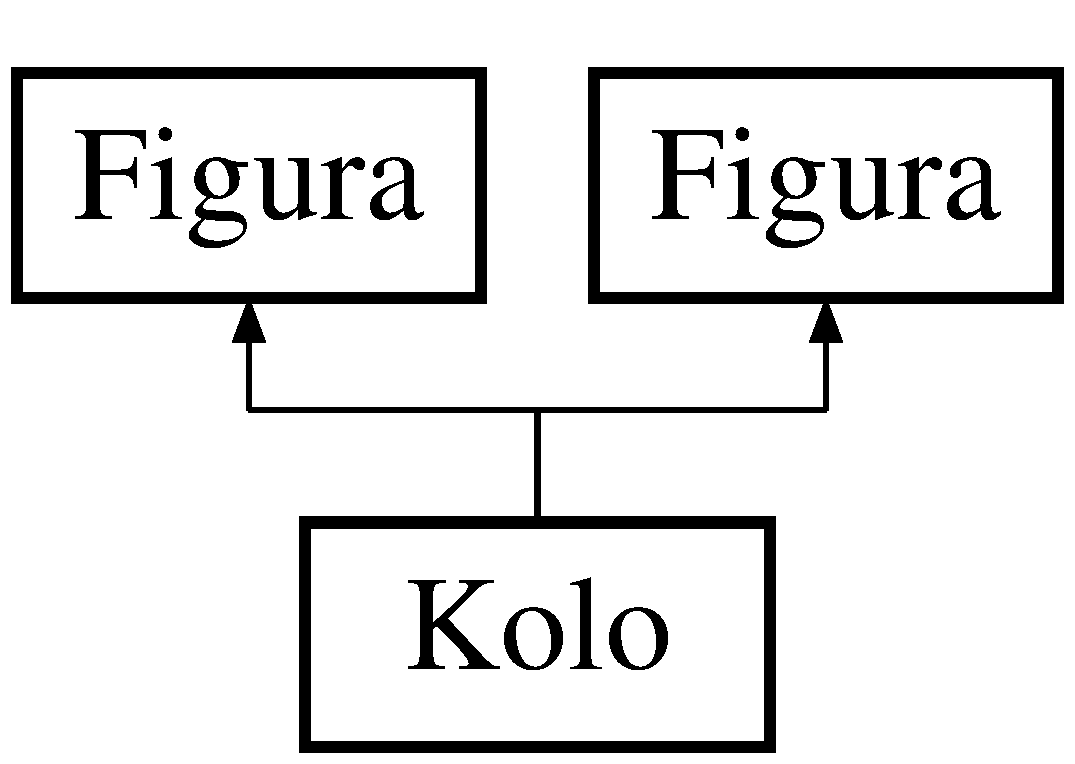
\includegraphics[height=2.000000cm]{d6/d1e/classKolo}
\end{center}
\end{figure}
\subsection*{Metody publiczne}
\begin{DoxyCompactItemize}
\item 
\hyperlink{classKolo_ae2e4cdea681bba2c90d0f5b5782a1a0b}{Kolo} ()
\item 
\hyperlink{classKolo_a4437f43801d28e21c7da14dba1a08b10}{Kolo} (float x\-\_\-, float y\-\_\-, float r\-\_\-)
\item 
\hyperlink{classKolo_adbfca387541fcfa2fa92f1d60b4a1adb}{$\sim$\-Kolo} ()
\item 
virtual void \hyperlink{classKolo_a9d16364f1efacc0b39933a2e9db3a9b8}{rysuj} ()
\item 
virtual float \hyperlink{classKolo_adf2327bc270704e26114bc70dbea76dd}{zwroc\-Rozmiar} ()
\item 
virtual bool \hyperlink{classKolo_ac07eacd65b94fb65ee5a7396e0d291c2}{czy\-Nalezydo\-Figury} (float \hyperlink{classFigura_ad640a05ebb1ddbf595124f0b31793e8a}{x}, float \hyperlink{classFigura_ab17e5953f2898eb729b2dc506640bce2}{y})
\item 
virtual bool \hyperlink{classKolo_a764c248ce1d8a6cbade93abb0b53b45c}{czy\-Kolizja} (\hyperlink{classFigura}{Figura} $\ast$druga)
\item 
virtual void \hyperlink{classKolo_a93c343ba7f2d41c18b4d9a6f9ac23894}{zmien\-Rozmiar} (float)
\item 
virtual float \hyperlink{classKolo_a1b27f5ce6fd9ae25b29025363ef5ff44}{zwroc\-Pole} ()
\item 
virtual void \hyperlink{classKolo_a7bcbafc8534dce8592adca0a146e4a4c}{zmien\-Pole} (float)
\item 
virtual double \hyperlink{classKolo_ac4635854f50604a0cf6f5055f0c20b1f}{zwrocodleglosc\-Do\-Kolizji} ()
\item 
virtual int \hyperlink{classKolo_aa374f8d794a4705b17372c9695e6b5b5}{zwroc\-Typ} ()
\item 
\hyperlink{classKolo_ae2e4cdea681bba2c90d0f5b5782a1a0b}{Kolo} ()
\item 
\hyperlink{classKolo_a4437f43801d28e21c7da14dba1a08b10}{Kolo} (float x\-\_\-, float y\-\_\-, float r\-\_\-)
\item 
\hyperlink{classKolo_adbfca387541fcfa2fa92f1d60b4a1adb}{$\sim$\-Kolo} ()
\item 
virtual void \hyperlink{classKolo_ab39849ea8257405a2c0aa60d138db1ac}{rysuj} ()
\item 
virtual float \hyperlink{classKolo_ad118d0c2ed1117b633a72226467eb427}{zwroc\-Rozmiar} ()
\item 
virtual bool \hyperlink{classKolo_a72ea08406dc57802251022ce4b3610af}{czy\-Nalezydo\-Figury} (float \hyperlink{classFigura_ad640a05ebb1ddbf595124f0b31793e8a}{x}, float \hyperlink{classFigura_ab17e5953f2898eb729b2dc506640bce2}{y})
\item 
virtual bool \hyperlink{classKolo_a6877ef8b09a94c8fd65a52e538821890}{czy\-Kolizja} (\hyperlink{classFigura}{Figura} $\ast$druga)
\item 
virtual void \hyperlink{classKolo_aa8f420ed4ebb1f905c78b3964e68e408}{zmien\-Rozmiar} (float)
\item 
virtual float \hyperlink{classKolo_ae23236b6d35139007f9d64e7f16a27d6}{zwroc\-Pole} ()
\item 
virtual void \hyperlink{classKolo_af634cf63538e8a04081d646749469f6b}{zmien\-Pole} (float)
\item 
virtual double \hyperlink{classKolo_ac432a050e65fbae273eb9b488247b8b4}{zwrocodleglosc\-Do\-Kolizji} ()
\item 
virtual int \hyperlink{classKolo_af413d5ccc6f715370feb50754e48307d}{zwroc\-Typ} ()
\end{DoxyCompactItemize}
\subsection*{Przyjaciele}
\begin{DoxyCompactItemize}
\item 
Q\-Data\-Stream \& \hyperlink{classKolo_aa61581e0ce86c42a2ee6e8bdeb1a62a6}{operator$<$$<$} (Q\-Data\-Stream \&stream, \hyperlink{classKolo}{Kolo} $\ast$kolo)
\item 
Q\-Data\-Stream \& \hyperlink{classKolo_a22f6faefdd5da21ac8da0b2774b6e315}{operator$>$$>$} (Q\-Data\-Stream \&stream, \hyperlink{classKolo}{Kolo} $\ast$kolo)
\item 
Q\-Data\-Stream \& \hyperlink{classKolo_a8434c0df2b3e44b1b0363ed8461c915f}{operator$<$$<$} (Q\-Data\-Stream \&stream, Q\-List$<$ \hyperlink{classKolo}{Kolo} $\ast$ $>$ \&lista\-Kol)
\item 
Q\-Data\-Stream \& \hyperlink{classKolo_a402d820c53425640a00c68b9f538ac2c}{operator$>$$>$} (Q\-Data\-Stream \&stream, Q\-List$<$ \hyperlink{classKolo}{Kolo} $\ast$ $>$ \&lista\-Kol)
\item 
Q\-Data\-Stream \& \hyperlink{classKolo_aa61581e0ce86c42a2ee6e8bdeb1a62a6}{operator$<$$<$} (Q\-Data\-Stream \&stream, \hyperlink{classKolo}{Kolo} $\ast$kolo)
\item 
Q\-Data\-Stream \& \hyperlink{classKolo_a22f6faefdd5da21ac8da0b2774b6e315}{operator$>$$>$} (Q\-Data\-Stream \&stream, \hyperlink{classKolo}{Kolo} $\ast$kolo)
\item 
Q\-Data\-Stream \& \hyperlink{classKolo_a8434c0df2b3e44b1b0363ed8461c915f}{operator$<$$<$} (Q\-Data\-Stream \&stream, Q\-List$<$ \hyperlink{classKolo}{Kolo} $\ast$ $>$ \&lista\-Kol)
\item 
Q\-Data\-Stream \& \hyperlink{classKolo_a402d820c53425640a00c68b9f538ac2c}{operator$>$$>$} (Q\-Data\-Stream \&stream, Q\-List$<$ \hyperlink{classKolo}{Kolo} $\ast$ $>$ \&lista\-Kol)
\end{DoxyCompactItemize}
\subsection*{Dodatkowe Dziedziczone Składowe}


\subsection{Dokumentacja konstruktora i destruktora}
\hypertarget{classKolo_ae2e4cdea681bba2c90d0f5b5782a1a0b}{\index{Kolo@{Kolo}!Kolo@{Kolo}}
\index{Kolo@{Kolo}!Kolo@{Kolo}}
\subsubsection[{Kolo}]{\setlength{\rightskip}{0pt plus 5cm}Kolo\-::\-Kolo (
\begin{DoxyParamCaption}
{}
\end{DoxyParamCaption}
)}}\label{classKolo_ae2e4cdea681bba2c90d0f5b5782a1a0b}
\hypertarget{classKolo_a4437f43801d28e21c7da14dba1a08b10}{\index{Kolo@{Kolo}!Kolo@{Kolo}}
\index{Kolo@{Kolo}!Kolo@{Kolo}}
\subsubsection[{Kolo}]{\setlength{\rightskip}{0pt plus 5cm}Kolo\-::\-Kolo (
\begin{DoxyParamCaption}
\item[{float}]{x\-\_\-, }
\item[{float}]{y\-\_\-, }
\item[{float}]{r\-\_\-}
\end{DoxyParamCaption}
)}}\label{classKolo_a4437f43801d28e21c7da14dba1a08b10}
\hypertarget{classKolo_adbfca387541fcfa2fa92f1d60b4a1adb}{\index{Kolo@{Kolo}!$\sim$\-Kolo@{$\sim$\-Kolo}}
\index{$\sim$\-Kolo@{$\sim$\-Kolo}!Kolo@{Kolo}}
\subsubsection[{$\sim$\-Kolo}]{\setlength{\rightskip}{0pt plus 5cm}Kolo\-::$\sim$\-Kolo (
\begin{DoxyParamCaption}
{}
\end{DoxyParamCaption}
)}}\label{classKolo_adbfca387541fcfa2fa92f1d60b4a1adb}
\hypertarget{classKolo_ae2e4cdea681bba2c90d0f5b5782a1a0b}{\index{Kolo@{Kolo}!Kolo@{Kolo}}
\index{Kolo@{Kolo}!Kolo@{Kolo}}
\subsubsection[{Kolo}]{\setlength{\rightskip}{0pt plus 5cm}Kolo\-::\-Kolo (
\begin{DoxyParamCaption}
{}
\end{DoxyParamCaption}
)}}\label{classKolo_ae2e4cdea681bba2c90d0f5b5782a1a0b}
\hypertarget{classKolo_a4437f43801d28e21c7da14dba1a08b10}{\index{Kolo@{Kolo}!Kolo@{Kolo}}
\index{Kolo@{Kolo}!Kolo@{Kolo}}
\subsubsection[{Kolo}]{\setlength{\rightskip}{0pt plus 5cm}Kolo\-::\-Kolo (
\begin{DoxyParamCaption}
\item[{float}]{x\-\_\-, }
\item[{float}]{y\-\_\-, }
\item[{float}]{r\-\_\-}
\end{DoxyParamCaption}
)}}\label{classKolo_a4437f43801d28e21c7da14dba1a08b10}
\hypertarget{classKolo_adbfca387541fcfa2fa92f1d60b4a1adb}{\index{Kolo@{Kolo}!$\sim$\-Kolo@{$\sim$\-Kolo}}
\index{$\sim$\-Kolo@{$\sim$\-Kolo}!Kolo@{Kolo}}
\subsubsection[{$\sim$\-Kolo}]{\setlength{\rightskip}{0pt plus 5cm}Kolo\-::$\sim$\-Kolo (
\begin{DoxyParamCaption}
{}
\end{DoxyParamCaption}
)}}\label{classKolo_adbfca387541fcfa2fa92f1d60b4a1adb}


\subsection{Dokumentacja funkcji składowych}
\hypertarget{classKolo_a764c248ce1d8a6cbade93abb0b53b45c}{\index{Kolo@{Kolo}!czy\-Kolizja@{czy\-Kolizja}}
\index{czy\-Kolizja@{czy\-Kolizja}!Kolo@{Kolo}}
\subsubsection[{czy\-Kolizja}]{\setlength{\rightskip}{0pt plus 5cm}bool Kolo\-::czy\-Kolizja (
\begin{DoxyParamCaption}
\item[{{\bf Figura} $\ast$}]{druga}
\end{DoxyParamCaption}
)\hspace{0.3cm}{\ttfamily [virtual]}}}\label{classKolo_a764c248ce1d8a6cbade93abb0b53b45c}


Implementuje \hyperlink{classFigura_a7a1cb0014aaaa276f8b17932c394b485}{Figura}.

\hypertarget{classKolo_a6877ef8b09a94c8fd65a52e538821890}{\index{Kolo@{Kolo}!czy\-Kolizja@{czy\-Kolizja}}
\index{czy\-Kolizja@{czy\-Kolizja}!Kolo@{Kolo}}
\subsubsection[{czy\-Kolizja}]{\setlength{\rightskip}{0pt plus 5cm}virtual bool Kolo\-::czy\-Kolizja (
\begin{DoxyParamCaption}
\item[{{\bf Figura} $\ast$}]{druga}
\end{DoxyParamCaption}
)\hspace{0.3cm}{\ttfamily [virtual]}}}\label{classKolo_a6877ef8b09a94c8fd65a52e538821890}


Implementuje \hyperlink{classFigura_a7a1cb0014aaaa276f8b17932c394b485}{Figura}.

\hypertarget{classKolo_ac07eacd65b94fb65ee5a7396e0d291c2}{\index{Kolo@{Kolo}!czy\-Nalezydo\-Figury@{czy\-Nalezydo\-Figury}}
\index{czy\-Nalezydo\-Figury@{czy\-Nalezydo\-Figury}!Kolo@{Kolo}}
\subsubsection[{czy\-Nalezydo\-Figury}]{\setlength{\rightskip}{0pt plus 5cm}bool Kolo\-::czy\-Nalezydo\-Figury (
\begin{DoxyParamCaption}
\item[{float}]{x, }
\item[{float}]{y}
\end{DoxyParamCaption}
)\hspace{0.3cm}{\ttfamily [virtual]}}}\label{classKolo_ac07eacd65b94fb65ee5a7396e0d291c2}


Implementuje \hyperlink{classFigura_a14f9ba21828b6292488e1fa12bf1b85f}{Figura}.

\hypertarget{classKolo_a72ea08406dc57802251022ce4b3610af}{\index{Kolo@{Kolo}!czy\-Nalezydo\-Figury@{czy\-Nalezydo\-Figury}}
\index{czy\-Nalezydo\-Figury@{czy\-Nalezydo\-Figury}!Kolo@{Kolo}}
\subsubsection[{czy\-Nalezydo\-Figury}]{\setlength{\rightskip}{0pt plus 5cm}virtual bool Kolo\-::czy\-Nalezydo\-Figury (
\begin{DoxyParamCaption}
\item[{float}]{x, }
\item[{float}]{y}
\end{DoxyParamCaption}
)\hspace{0.3cm}{\ttfamily [virtual]}}}\label{classKolo_a72ea08406dc57802251022ce4b3610af}


Implementuje \hyperlink{classFigura_a14f9ba21828b6292488e1fa12bf1b85f}{Figura}.

\hypertarget{classKolo_ab39849ea8257405a2c0aa60d138db1ac}{\index{Kolo@{Kolo}!rysuj@{rysuj}}
\index{rysuj@{rysuj}!Kolo@{Kolo}}
\subsubsection[{rysuj}]{\setlength{\rightskip}{0pt plus 5cm}virtual void Kolo\-::rysuj (
\begin{DoxyParamCaption}
{}
\end{DoxyParamCaption}
)\hspace{0.3cm}{\ttfamily [virtual]}}}\label{classKolo_ab39849ea8257405a2c0aa60d138db1ac}


Implementuje \hyperlink{classFigura_a6ec035fbeb95129af6ca64d2adff7651}{Figura}.

\hypertarget{classKolo_a9d16364f1efacc0b39933a2e9db3a9b8}{\index{Kolo@{Kolo}!rysuj@{rysuj}}
\index{rysuj@{rysuj}!Kolo@{Kolo}}
\subsubsection[{rysuj}]{\setlength{\rightskip}{0pt plus 5cm}void Kolo\-::rysuj (
\begin{DoxyParamCaption}
{}
\end{DoxyParamCaption}
)\hspace{0.3cm}{\ttfamily [virtual]}}}\label{classKolo_a9d16364f1efacc0b39933a2e9db3a9b8}


Implementuje \hyperlink{classFigura_a6ec035fbeb95129af6ca64d2adff7651}{Figura}.

\hypertarget{classKolo_af634cf63538e8a04081d646749469f6b}{\index{Kolo@{Kolo}!zmien\-Pole@{zmien\-Pole}}
\index{zmien\-Pole@{zmien\-Pole}!Kolo@{Kolo}}
\subsubsection[{zmien\-Pole}]{\setlength{\rightskip}{0pt plus 5cm}virtual void Kolo\-::zmien\-Pole (
\begin{DoxyParamCaption}
\item[{float}]{}
\end{DoxyParamCaption}
)\hspace{0.3cm}{\ttfamily [virtual]}}}\label{classKolo_af634cf63538e8a04081d646749469f6b}


Implementuje \hyperlink{classFigura_aad1198cc826aa6b3036454fd4f3bb5b3}{Figura}.

\hypertarget{classKolo_a7bcbafc8534dce8592adca0a146e4a4c}{\index{Kolo@{Kolo}!zmien\-Pole@{zmien\-Pole}}
\index{zmien\-Pole@{zmien\-Pole}!Kolo@{Kolo}}
\subsubsection[{zmien\-Pole}]{\setlength{\rightskip}{0pt plus 5cm}void Kolo\-::zmien\-Pole (
\begin{DoxyParamCaption}
\item[{float}]{dp}
\end{DoxyParamCaption}
)\hspace{0.3cm}{\ttfamily [virtual]}}}\label{classKolo_a7bcbafc8534dce8592adca0a146e4a4c}


Implementuje \hyperlink{classFigura_aad1198cc826aa6b3036454fd4f3bb5b3}{Figura}.

\hypertarget{classKolo_a93c343ba7f2d41c18b4d9a6f9ac23894}{\index{Kolo@{Kolo}!zmien\-Rozmiar@{zmien\-Rozmiar}}
\index{zmien\-Rozmiar@{zmien\-Rozmiar}!Kolo@{Kolo}}
\subsubsection[{zmien\-Rozmiar}]{\setlength{\rightskip}{0pt plus 5cm}void Kolo\-::zmien\-Rozmiar (
\begin{DoxyParamCaption}
\item[{float}]{dr}
\end{DoxyParamCaption}
)\hspace{0.3cm}{\ttfamily [virtual]}}}\label{classKolo_a93c343ba7f2d41c18b4d9a6f9ac23894}


Implementuje \hyperlink{classFigura_a7ea2c8b450129878f4347404b8834c6b}{Figura}.

\hypertarget{classKolo_aa8f420ed4ebb1f905c78b3964e68e408}{\index{Kolo@{Kolo}!zmien\-Rozmiar@{zmien\-Rozmiar}}
\index{zmien\-Rozmiar@{zmien\-Rozmiar}!Kolo@{Kolo}}
\subsubsection[{zmien\-Rozmiar}]{\setlength{\rightskip}{0pt plus 5cm}virtual void Kolo\-::zmien\-Rozmiar (
\begin{DoxyParamCaption}
\item[{float}]{}
\end{DoxyParamCaption}
)\hspace{0.3cm}{\ttfamily [virtual]}}}\label{classKolo_aa8f420ed4ebb1f905c78b3964e68e408}


Implementuje \hyperlink{classFigura_a7ea2c8b450129878f4347404b8834c6b}{Figura}.

\hypertarget{classKolo_ac4635854f50604a0cf6f5055f0c20b1f}{\index{Kolo@{Kolo}!zwrocodleglosc\-Do\-Kolizji@{zwrocodleglosc\-Do\-Kolizji}}
\index{zwrocodleglosc\-Do\-Kolizji@{zwrocodleglosc\-Do\-Kolizji}!Kolo@{Kolo}}
\subsubsection[{zwrocodleglosc\-Do\-Kolizji}]{\setlength{\rightskip}{0pt plus 5cm}double Kolo\-::zwrocodleglosc\-Do\-Kolizji (
\begin{DoxyParamCaption}
{}
\end{DoxyParamCaption}
)\hspace{0.3cm}{\ttfamily [virtual]}}}\label{classKolo_ac4635854f50604a0cf6f5055f0c20b1f}


Implementuje \hyperlink{classFigura_a3e534b43a279aeec36c5b28ac731e0f8}{Figura}.

\hypertarget{classKolo_ac432a050e65fbae273eb9b488247b8b4}{\index{Kolo@{Kolo}!zwrocodleglosc\-Do\-Kolizji@{zwrocodleglosc\-Do\-Kolizji}}
\index{zwrocodleglosc\-Do\-Kolizji@{zwrocodleglosc\-Do\-Kolizji}!Kolo@{Kolo}}
\subsubsection[{zwrocodleglosc\-Do\-Kolizji}]{\setlength{\rightskip}{0pt plus 5cm}virtual double Kolo\-::zwrocodleglosc\-Do\-Kolizji (
\begin{DoxyParamCaption}
{}
\end{DoxyParamCaption}
)\hspace{0.3cm}{\ttfamily [virtual]}}}\label{classKolo_ac432a050e65fbae273eb9b488247b8b4}


Implementuje \hyperlink{classFigura_a3e534b43a279aeec36c5b28ac731e0f8}{Figura}.

\hypertarget{classKolo_ae23236b6d35139007f9d64e7f16a27d6}{\index{Kolo@{Kolo}!zwroc\-Pole@{zwroc\-Pole}}
\index{zwroc\-Pole@{zwroc\-Pole}!Kolo@{Kolo}}
\subsubsection[{zwroc\-Pole}]{\setlength{\rightskip}{0pt plus 5cm}virtual float Kolo\-::zwroc\-Pole (
\begin{DoxyParamCaption}
{}
\end{DoxyParamCaption}
)\hspace{0.3cm}{\ttfamily [virtual]}}}\label{classKolo_ae23236b6d35139007f9d64e7f16a27d6}


Implementuje \hyperlink{classFigura_a78861f3fce7e615ba30b47aa1cdcebec}{Figura}.

\hypertarget{classKolo_a1b27f5ce6fd9ae25b29025363ef5ff44}{\index{Kolo@{Kolo}!zwroc\-Pole@{zwroc\-Pole}}
\index{zwroc\-Pole@{zwroc\-Pole}!Kolo@{Kolo}}
\subsubsection[{zwroc\-Pole}]{\setlength{\rightskip}{0pt plus 5cm}float Kolo\-::zwroc\-Pole (
\begin{DoxyParamCaption}
{}
\end{DoxyParamCaption}
)\hspace{0.3cm}{\ttfamily [virtual]}}}\label{classKolo_a1b27f5ce6fd9ae25b29025363ef5ff44}


Implementuje \hyperlink{classFigura_a78861f3fce7e615ba30b47aa1cdcebec}{Figura}.

\hypertarget{classKolo_adf2327bc270704e26114bc70dbea76dd}{\index{Kolo@{Kolo}!zwroc\-Rozmiar@{zwroc\-Rozmiar}}
\index{zwroc\-Rozmiar@{zwroc\-Rozmiar}!Kolo@{Kolo}}
\subsubsection[{zwroc\-Rozmiar}]{\setlength{\rightskip}{0pt plus 5cm}float Kolo\-::zwroc\-Rozmiar (
\begin{DoxyParamCaption}
{}
\end{DoxyParamCaption}
)\hspace{0.3cm}{\ttfamily [virtual]}}}\label{classKolo_adf2327bc270704e26114bc70dbea76dd}


Implementuje \hyperlink{classFigura_aaeb587028aafd028e134079c249b0c88}{Figura}.

\hypertarget{classKolo_ad118d0c2ed1117b633a72226467eb427}{\index{Kolo@{Kolo}!zwroc\-Rozmiar@{zwroc\-Rozmiar}}
\index{zwroc\-Rozmiar@{zwroc\-Rozmiar}!Kolo@{Kolo}}
\subsubsection[{zwroc\-Rozmiar}]{\setlength{\rightskip}{0pt plus 5cm}virtual float Kolo\-::zwroc\-Rozmiar (
\begin{DoxyParamCaption}
{}
\end{DoxyParamCaption}
)\hspace{0.3cm}{\ttfamily [virtual]}}}\label{classKolo_ad118d0c2ed1117b633a72226467eb427}


Implementuje \hyperlink{classFigura_aaeb587028aafd028e134079c249b0c88}{Figura}.

\hypertarget{classKolo_af413d5ccc6f715370feb50754e48307d}{\index{Kolo@{Kolo}!zwroc\-Typ@{zwroc\-Typ}}
\index{zwroc\-Typ@{zwroc\-Typ}!Kolo@{Kolo}}
\subsubsection[{zwroc\-Typ}]{\setlength{\rightskip}{0pt plus 5cm}virtual int Kolo\-::zwroc\-Typ (
\begin{DoxyParamCaption}
{}
\end{DoxyParamCaption}
)\hspace{0.3cm}{\ttfamily [virtual]}}}\label{classKolo_af413d5ccc6f715370feb50754e48307d}


Implementuje \hyperlink{classFigura_ab04732de63f17d4c3776990d24897db7}{Figura}.

\hypertarget{classKolo_aa374f8d794a4705b17372c9695e6b5b5}{\index{Kolo@{Kolo}!zwroc\-Typ@{zwroc\-Typ}}
\index{zwroc\-Typ@{zwroc\-Typ}!Kolo@{Kolo}}
\subsubsection[{zwroc\-Typ}]{\setlength{\rightskip}{0pt plus 5cm}int Kolo\-::zwroc\-Typ (
\begin{DoxyParamCaption}
{}
\end{DoxyParamCaption}
)\hspace{0.3cm}{\ttfamily [virtual]}}}\label{classKolo_aa374f8d794a4705b17372c9695e6b5b5}


Implementuje \hyperlink{classFigura_ab04732de63f17d4c3776990d24897db7}{Figura}.



\subsection{Dokumentacja przyjaciół i funkcji związanych}
\hypertarget{classKolo_aa61581e0ce86c42a2ee6e8bdeb1a62a6}{\index{Kolo@{Kolo}!operator$<$$<$@{operator$<$$<$}}
\index{operator$<$$<$@{operator$<$$<$}!Kolo@{Kolo}}
\subsubsection[{operator$<$$<$}]{\setlength{\rightskip}{0pt plus 5cm}Q\-Data\-Stream\& operator$<$$<$ (
\begin{DoxyParamCaption}
\item[{Q\-Data\-Stream \&}]{stream, }
\item[{{\bf Kolo} $\ast$}]{kolo}
\end{DoxyParamCaption}
)\hspace{0.3cm}{\ttfamily [friend]}}}\label{classKolo_aa61581e0ce86c42a2ee6e8bdeb1a62a6}
\hypertarget{classKolo_aa61581e0ce86c42a2ee6e8bdeb1a62a6}{\index{Kolo@{Kolo}!operator$<$$<$@{operator$<$$<$}}
\index{operator$<$$<$@{operator$<$$<$}!Kolo@{Kolo}}
\subsubsection[{operator$<$$<$}]{\setlength{\rightskip}{0pt plus 5cm}Q\-Data\-Stream\& operator$<$$<$ (
\begin{DoxyParamCaption}
\item[{Q\-Data\-Stream \&}]{stream, }
\item[{{\bf Kolo} $\ast$}]{kolo}
\end{DoxyParamCaption}
)\hspace{0.3cm}{\ttfamily [friend]}}}\label{classKolo_aa61581e0ce86c42a2ee6e8bdeb1a62a6}
\hypertarget{classKolo_a8434c0df2b3e44b1b0363ed8461c915f}{\index{Kolo@{Kolo}!operator$<$$<$@{operator$<$$<$}}
\index{operator$<$$<$@{operator$<$$<$}!Kolo@{Kolo}}
\subsubsection[{operator$<$$<$}]{\setlength{\rightskip}{0pt plus 5cm}Q\-Data\-Stream\& operator$<$$<$ (
\begin{DoxyParamCaption}
\item[{Q\-Data\-Stream \&}]{stream, }
\item[{Q\-List$<$ {\bf Kolo} $\ast$ $>$ \&}]{lista\-Kol}
\end{DoxyParamCaption}
)\hspace{0.3cm}{\ttfamily [friend]}}}\label{classKolo_a8434c0df2b3e44b1b0363ed8461c915f}
\hypertarget{classKolo_a8434c0df2b3e44b1b0363ed8461c915f}{\index{Kolo@{Kolo}!operator$<$$<$@{operator$<$$<$}}
\index{operator$<$$<$@{operator$<$$<$}!Kolo@{Kolo}}
\subsubsection[{operator$<$$<$}]{\setlength{\rightskip}{0pt plus 5cm}Q\-Data\-Stream\& operator$<$$<$ (
\begin{DoxyParamCaption}
\item[{Q\-Data\-Stream \&}]{stream, }
\item[{Q\-List$<$ {\bf Kolo} $\ast$ $>$ \&}]{lista\-Kol}
\end{DoxyParamCaption}
)\hspace{0.3cm}{\ttfamily [friend]}}}\label{classKolo_a8434c0df2b3e44b1b0363ed8461c915f}
\hypertarget{classKolo_a22f6faefdd5da21ac8da0b2774b6e315}{\index{Kolo@{Kolo}!operator$>$$>$@{operator$>$$>$}}
\index{operator$>$$>$@{operator$>$$>$}!Kolo@{Kolo}}
\subsubsection[{operator$>$$>$}]{\setlength{\rightskip}{0pt plus 5cm}Q\-Data\-Stream\& operator$>$$>$ (
\begin{DoxyParamCaption}
\item[{Q\-Data\-Stream \&}]{stream, }
\item[{{\bf Kolo} $\ast$}]{kolo}
\end{DoxyParamCaption}
)\hspace{0.3cm}{\ttfamily [friend]}}}\label{classKolo_a22f6faefdd5da21ac8da0b2774b6e315}
\hypertarget{classKolo_a22f6faefdd5da21ac8da0b2774b6e315}{\index{Kolo@{Kolo}!operator$>$$>$@{operator$>$$>$}}
\index{operator$>$$>$@{operator$>$$>$}!Kolo@{Kolo}}
\subsubsection[{operator$>$$>$}]{\setlength{\rightskip}{0pt plus 5cm}Q\-Data\-Stream\& operator$>$$>$ (
\begin{DoxyParamCaption}
\item[{Q\-Data\-Stream \&}]{stream, }
\item[{{\bf Kolo} $\ast$}]{kolo}
\end{DoxyParamCaption}
)\hspace{0.3cm}{\ttfamily [friend]}}}\label{classKolo_a22f6faefdd5da21ac8da0b2774b6e315}
\hypertarget{classKolo_a402d820c53425640a00c68b9f538ac2c}{\index{Kolo@{Kolo}!operator$>$$>$@{operator$>$$>$}}
\index{operator$>$$>$@{operator$>$$>$}!Kolo@{Kolo}}
\subsubsection[{operator$>$$>$}]{\setlength{\rightskip}{0pt plus 5cm}Q\-Data\-Stream\& operator$>$$>$ (
\begin{DoxyParamCaption}
\item[{Q\-Data\-Stream \&}]{stream, }
\item[{Q\-List$<$ {\bf Kolo} $\ast$ $>$ \&}]{lista\-Kol}
\end{DoxyParamCaption}
)\hspace{0.3cm}{\ttfamily [friend]}}}\label{classKolo_a402d820c53425640a00c68b9f538ac2c}
\hypertarget{classKolo_a402d820c53425640a00c68b9f538ac2c}{\index{Kolo@{Kolo}!operator$>$$>$@{operator$>$$>$}}
\index{operator$>$$>$@{operator$>$$>$}!Kolo@{Kolo}}
\subsubsection[{operator$>$$>$}]{\setlength{\rightskip}{0pt plus 5cm}Q\-Data\-Stream\& operator$>$$>$ (
\begin{DoxyParamCaption}
\item[{Q\-Data\-Stream \&}]{stream, }
\item[{Q\-List$<$ {\bf Kolo} $\ast$ $>$ \&}]{lista\-Kol}
\end{DoxyParamCaption}
)\hspace{0.3cm}{\ttfamily [friend]}}}\label{classKolo_a402d820c53425640a00c68b9f538ac2c}


Dokumentacja dla tej klasy została wygenerowana z plików\-:\begin{DoxyCompactItemize}
\item 
Gra\-Figury/\hyperlink{GraFigury_2kolo_8h}{kolo.\-h}\item 
Gra\-Figury/\hyperlink{GraFigury_2kolo_8cpp}{kolo.\-cpp}\end{DoxyCompactItemize}

\hypertarget{classKwadrat}{\section{Dokumentacja klasy Kwadrat}
\label{classKwadrat}\index{Kwadrat@{Kwadrat}}
}


{\ttfamily \#include $<$kwadrat.\-h$>$}

Diagram dziedziczenia dla Kwadrat\begin{figure}[H]
\begin{center}
\leavevmode
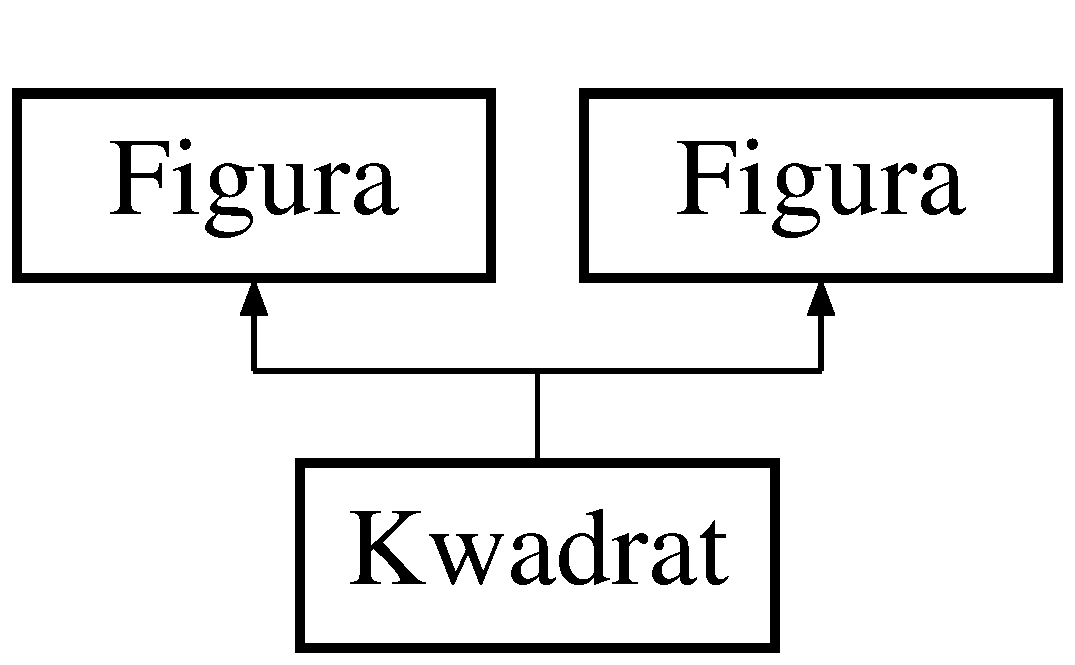
\includegraphics[height=2.000000cm]{classKwadrat}
\end{center}
\end{figure}
\subsection*{Metody publiczne}
\begin{DoxyCompactItemize}
\item 
\hyperlink{classKwadrat_a7c105c83f59b0fa65af35714f4f55189}{Kwadrat} ()
\item 
\hyperlink{classKwadrat_a4cd1adc4069cc35048fdbf2eeaa8fdfd}{Kwadrat} (float x\-\_\-, float y\-\_\-, float a\-\_\-)
\item 
\hyperlink{classKwadrat_a0840295ae2e7d75daba30640fa1c1b56}{$\sim$\-Kwadrat} ()
\item 
virtual void \hyperlink{classKwadrat_a1e9cfa05c327d73f48c4ddd2f7b363db}{rysuj} ()
\item 
virtual float \hyperlink{classKwadrat_abbbda79a7812a6c8e9dcadfaa248982c}{zwroc\-Rozmiar} ()
\item 
virtual bool \hyperlink{classKwadrat_aaa67e4e84772b2670215a725d5711784}{czy\-Nalezydo\-Figury} (float \hyperlink{classFigura_ad640a05ebb1ddbf595124f0b31793e8a}{x}, float \hyperlink{classFigura_ab17e5953f2898eb729b2dc506640bce2}{y})
\item 
virtual bool \hyperlink{classKwadrat_ad0edd62e4fa3a541f6d39f902dd097cd}{czy\-Kolizja} (\hyperlink{classFigura}{Figura} $\ast$druga)
\item 
virtual void \hyperlink{classKwadrat_ad081e004bc8ba64d18989934ac95e272}{zmien\-Rozmiar} (float)
\item 
virtual float \hyperlink{classKwadrat_a1ad16348ebef01a8040e71025356e554}{zwroc\-Pole} ()
\item 
virtual void \hyperlink{classKwadrat_aa88d774d1a32bd8ceba12e9f2c003f8a}{zmien\-Pole} (float)
\item 
virtual double \hyperlink{classKwadrat_ab077c930d3ad276dc981615aed700b98}{zwrocodleglosc\-Do\-Kolizji} ()
\item 
virtual int \hyperlink{classKwadrat_a4fe24ee70d53bade8c1d5c29a4d9e028}{zwroc\-Typ} ()
\item 
\hyperlink{classKwadrat_a7c105c83f59b0fa65af35714f4f55189}{Kwadrat} ()
\item 
\hyperlink{classKwadrat_a4cd1adc4069cc35048fdbf2eeaa8fdfd}{Kwadrat} (float x\-\_\-, float y\-\_\-, float a\-\_\-)
\item 
\hyperlink{classKwadrat_a0840295ae2e7d75daba30640fa1c1b56}{$\sim$\-Kwadrat} ()
\item 
virtual void \hyperlink{classKwadrat_a2aa3729d2a139f6c8bf61c734a53f920}{rysuj} ()
\item 
virtual float \hyperlink{classKwadrat_a2cd11e92113cab623bf2fbee5e983da9}{zwroc\-Rozmiar} ()
\item 
virtual bool \hyperlink{classKwadrat_ad2eea84aafada7c9f9a6deea1d28dd0b}{czy\-Nalezydo\-Figury} (float \hyperlink{classFigura_ad640a05ebb1ddbf595124f0b31793e8a}{x}, float \hyperlink{classFigura_ab17e5953f2898eb729b2dc506640bce2}{y})
\item 
virtual bool \hyperlink{classKwadrat_a892c42c9fe7265a8bf5209f2dac0291d}{czy\-Kolizja} (\hyperlink{classFigura}{Figura} $\ast$druga)
\item 
virtual void \hyperlink{classKwadrat_a5053f4a588bb04063c5b72398450f006}{zmien\-Rozmiar} (float)
\item 
virtual float \hyperlink{classKwadrat_a70746db00ffc11e8c587ad188e3c9f43}{zwroc\-Pole} ()
\item 
virtual void \hyperlink{classKwadrat_ad4aa4af07a2567679cea1a2aff08e157}{zmien\-Pole} (float)
\item 
virtual double \hyperlink{classKwadrat_a4349f00bc44e9848a495045fafea259b}{zwrocodleglosc\-Do\-Kolizji} ()
\item 
virtual int \hyperlink{classKwadrat_a496886971ae7c8987edb607cfde3823f}{zwroc\-Typ} ()
\end{DoxyCompactItemize}
\subsection*{Dodatkowe Dziedziczone Składowe}


\subsection{Dokumentacja konstruktora i destruktora}
\hypertarget{classKwadrat_a7c105c83f59b0fa65af35714f4f55189}{\index{Kwadrat@{Kwadrat}!Kwadrat@{Kwadrat}}
\index{Kwadrat@{Kwadrat}!Kwadrat@{Kwadrat}}
\subsubsection[{Kwadrat}]{\setlength{\rightskip}{0pt plus 5cm}Kwadrat\-::\-Kwadrat (
\begin{DoxyParamCaption}
{}
\end{DoxyParamCaption}
)}}\label{classKwadrat_a7c105c83f59b0fa65af35714f4f55189}
\hypertarget{classKwadrat_a4cd1adc4069cc35048fdbf2eeaa8fdfd}{\index{Kwadrat@{Kwadrat}!Kwadrat@{Kwadrat}}
\index{Kwadrat@{Kwadrat}!Kwadrat@{Kwadrat}}
\subsubsection[{Kwadrat}]{\setlength{\rightskip}{0pt plus 5cm}Kwadrat\-::\-Kwadrat (
\begin{DoxyParamCaption}
\item[{float}]{x\-\_\-, }
\item[{float}]{y\-\_\-, }
\item[{float}]{a\-\_\-}
\end{DoxyParamCaption}
)}}\label{classKwadrat_a4cd1adc4069cc35048fdbf2eeaa8fdfd}
\hypertarget{classKwadrat_a0840295ae2e7d75daba30640fa1c1b56}{\index{Kwadrat@{Kwadrat}!$\sim$\-Kwadrat@{$\sim$\-Kwadrat}}
\index{$\sim$\-Kwadrat@{$\sim$\-Kwadrat}!Kwadrat@{Kwadrat}}
\subsubsection[{$\sim$\-Kwadrat}]{\setlength{\rightskip}{0pt plus 5cm}Kwadrat\-::$\sim$\-Kwadrat (
\begin{DoxyParamCaption}
{}
\end{DoxyParamCaption}
)}}\label{classKwadrat_a0840295ae2e7d75daba30640fa1c1b56}
\hypertarget{classKwadrat_a7c105c83f59b0fa65af35714f4f55189}{\index{Kwadrat@{Kwadrat}!Kwadrat@{Kwadrat}}
\index{Kwadrat@{Kwadrat}!Kwadrat@{Kwadrat}}
\subsubsection[{Kwadrat}]{\setlength{\rightskip}{0pt plus 5cm}Kwadrat\-::\-Kwadrat (
\begin{DoxyParamCaption}
{}
\end{DoxyParamCaption}
)}}\label{classKwadrat_a7c105c83f59b0fa65af35714f4f55189}
\hypertarget{classKwadrat_a4cd1adc4069cc35048fdbf2eeaa8fdfd}{\index{Kwadrat@{Kwadrat}!Kwadrat@{Kwadrat}}
\index{Kwadrat@{Kwadrat}!Kwadrat@{Kwadrat}}
\subsubsection[{Kwadrat}]{\setlength{\rightskip}{0pt plus 5cm}Kwadrat\-::\-Kwadrat (
\begin{DoxyParamCaption}
\item[{float}]{x\-\_\-, }
\item[{float}]{y\-\_\-, }
\item[{float}]{a\-\_\-}
\end{DoxyParamCaption}
)}}\label{classKwadrat_a4cd1adc4069cc35048fdbf2eeaa8fdfd}
\hypertarget{classKwadrat_a0840295ae2e7d75daba30640fa1c1b56}{\index{Kwadrat@{Kwadrat}!$\sim$\-Kwadrat@{$\sim$\-Kwadrat}}
\index{$\sim$\-Kwadrat@{$\sim$\-Kwadrat}!Kwadrat@{Kwadrat}}
\subsubsection[{$\sim$\-Kwadrat}]{\setlength{\rightskip}{0pt plus 5cm}Kwadrat\-::$\sim$\-Kwadrat (
\begin{DoxyParamCaption}
{}
\end{DoxyParamCaption}
)}}\label{classKwadrat_a0840295ae2e7d75daba30640fa1c1b56}


\subsection{Dokumentacja funkcji składowych}
\hypertarget{classKwadrat_ad0edd62e4fa3a541f6d39f902dd097cd}{\index{Kwadrat@{Kwadrat}!czy\-Kolizja@{czy\-Kolizja}}
\index{czy\-Kolizja@{czy\-Kolizja}!Kwadrat@{Kwadrat}}
\subsubsection[{czy\-Kolizja}]{\setlength{\rightskip}{0pt plus 5cm}bool Kwadrat\-::czy\-Kolizja (
\begin{DoxyParamCaption}
\item[{{\bf Figura} $\ast$}]{druga}
\end{DoxyParamCaption}
)\hspace{0.3cm}{\ttfamily [virtual]}}}\label{classKwadrat_ad0edd62e4fa3a541f6d39f902dd097cd}


Implementuje \hyperlink{classFigura_a7a1cb0014aaaa276f8b17932c394b485}{Figura}.

\hypertarget{classKwadrat_a892c42c9fe7265a8bf5209f2dac0291d}{\index{Kwadrat@{Kwadrat}!czy\-Kolizja@{czy\-Kolizja}}
\index{czy\-Kolizja@{czy\-Kolizja}!Kwadrat@{Kwadrat}}
\subsubsection[{czy\-Kolizja}]{\setlength{\rightskip}{0pt plus 5cm}virtual bool Kwadrat\-::czy\-Kolizja (
\begin{DoxyParamCaption}
\item[{{\bf Figura} $\ast$}]{druga}
\end{DoxyParamCaption}
)\hspace{0.3cm}{\ttfamily [virtual]}}}\label{classKwadrat_a892c42c9fe7265a8bf5209f2dac0291d}


Implementuje \hyperlink{classFigura_a7a1cb0014aaaa276f8b17932c394b485}{Figura}.

\hypertarget{classKwadrat_aaa67e4e84772b2670215a725d5711784}{\index{Kwadrat@{Kwadrat}!czy\-Nalezydo\-Figury@{czy\-Nalezydo\-Figury}}
\index{czy\-Nalezydo\-Figury@{czy\-Nalezydo\-Figury}!Kwadrat@{Kwadrat}}
\subsubsection[{czy\-Nalezydo\-Figury}]{\setlength{\rightskip}{0pt plus 5cm}bool Kwadrat\-::czy\-Nalezydo\-Figury (
\begin{DoxyParamCaption}
\item[{float}]{x, }
\item[{float}]{y}
\end{DoxyParamCaption}
)\hspace{0.3cm}{\ttfamily [virtual]}}}\label{classKwadrat_aaa67e4e84772b2670215a725d5711784}


Implementuje \hyperlink{classFigura_a14f9ba21828b6292488e1fa12bf1b85f}{Figura}.

\hypertarget{classKwadrat_ad2eea84aafada7c9f9a6deea1d28dd0b}{\index{Kwadrat@{Kwadrat}!czy\-Nalezydo\-Figury@{czy\-Nalezydo\-Figury}}
\index{czy\-Nalezydo\-Figury@{czy\-Nalezydo\-Figury}!Kwadrat@{Kwadrat}}
\subsubsection[{czy\-Nalezydo\-Figury}]{\setlength{\rightskip}{0pt plus 5cm}virtual bool Kwadrat\-::czy\-Nalezydo\-Figury (
\begin{DoxyParamCaption}
\item[{float}]{x, }
\item[{float}]{y}
\end{DoxyParamCaption}
)\hspace{0.3cm}{\ttfamily [virtual]}}}\label{classKwadrat_ad2eea84aafada7c9f9a6deea1d28dd0b}


Implementuje \hyperlink{classFigura_a14f9ba21828b6292488e1fa12bf1b85f}{Figura}.

\hypertarget{classKwadrat_a2aa3729d2a139f6c8bf61c734a53f920}{\index{Kwadrat@{Kwadrat}!rysuj@{rysuj}}
\index{rysuj@{rysuj}!Kwadrat@{Kwadrat}}
\subsubsection[{rysuj}]{\setlength{\rightskip}{0pt plus 5cm}virtual void Kwadrat\-::rysuj (
\begin{DoxyParamCaption}
{}
\end{DoxyParamCaption}
)\hspace{0.3cm}{\ttfamily [virtual]}}}\label{classKwadrat_a2aa3729d2a139f6c8bf61c734a53f920}


Implementuje \hyperlink{classFigura_a6ec035fbeb95129af6ca64d2adff7651}{Figura}.

\hypertarget{classKwadrat_a1e9cfa05c327d73f48c4ddd2f7b363db}{\index{Kwadrat@{Kwadrat}!rysuj@{rysuj}}
\index{rysuj@{rysuj}!Kwadrat@{Kwadrat}}
\subsubsection[{rysuj}]{\setlength{\rightskip}{0pt plus 5cm}void Kwadrat\-::rysuj (
\begin{DoxyParamCaption}
{}
\end{DoxyParamCaption}
)\hspace{0.3cm}{\ttfamily [virtual]}}}\label{classKwadrat_a1e9cfa05c327d73f48c4ddd2f7b363db}


Implementuje \hyperlink{classFigura_a6ec035fbeb95129af6ca64d2adff7651}{Figura}.

\hypertarget{classKwadrat_ad4aa4af07a2567679cea1a2aff08e157}{\index{Kwadrat@{Kwadrat}!zmien\-Pole@{zmien\-Pole}}
\index{zmien\-Pole@{zmien\-Pole}!Kwadrat@{Kwadrat}}
\subsubsection[{zmien\-Pole}]{\setlength{\rightskip}{0pt plus 5cm}virtual void Kwadrat\-::zmien\-Pole (
\begin{DoxyParamCaption}
\item[{float}]{}
\end{DoxyParamCaption}
)\hspace{0.3cm}{\ttfamily [virtual]}}}\label{classKwadrat_ad4aa4af07a2567679cea1a2aff08e157}


Implementuje \hyperlink{classFigura_aad1198cc826aa6b3036454fd4f3bb5b3}{Figura}.

\hypertarget{classKwadrat_aa88d774d1a32bd8ceba12e9f2c003f8a}{\index{Kwadrat@{Kwadrat}!zmien\-Pole@{zmien\-Pole}}
\index{zmien\-Pole@{zmien\-Pole}!Kwadrat@{Kwadrat}}
\subsubsection[{zmien\-Pole}]{\setlength{\rightskip}{0pt plus 5cm}void Kwadrat\-::zmien\-Pole (
\begin{DoxyParamCaption}
\item[{float}]{dp}
\end{DoxyParamCaption}
)\hspace{0.3cm}{\ttfamily [virtual]}}}\label{classKwadrat_aa88d774d1a32bd8ceba12e9f2c003f8a}


Implementuje \hyperlink{classFigura_aad1198cc826aa6b3036454fd4f3bb5b3}{Figura}.

\hypertarget{classKwadrat_ad081e004bc8ba64d18989934ac95e272}{\index{Kwadrat@{Kwadrat}!zmien\-Rozmiar@{zmien\-Rozmiar}}
\index{zmien\-Rozmiar@{zmien\-Rozmiar}!Kwadrat@{Kwadrat}}
\subsubsection[{zmien\-Rozmiar}]{\setlength{\rightskip}{0pt plus 5cm}void Kwadrat\-::zmien\-Rozmiar (
\begin{DoxyParamCaption}
\item[{float}]{dr}
\end{DoxyParamCaption}
)\hspace{0.3cm}{\ttfamily [virtual]}}}\label{classKwadrat_ad081e004bc8ba64d18989934ac95e272}


Implementuje \hyperlink{classFigura_a7ea2c8b450129878f4347404b8834c6b}{Figura}.

\hypertarget{classKwadrat_a5053f4a588bb04063c5b72398450f006}{\index{Kwadrat@{Kwadrat}!zmien\-Rozmiar@{zmien\-Rozmiar}}
\index{zmien\-Rozmiar@{zmien\-Rozmiar}!Kwadrat@{Kwadrat}}
\subsubsection[{zmien\-Rozmiar}]{\setlength{\rightskip}{0pt plus 5cm}virtual void Kwadrat\-::zmien\-Rozmiar (
\begin{DoxyParamCaption}
\item[{float}]{}
\end{DoxyParamCaption}
)\hspace{0.3cm}{\ttfamily [virtual]}}}\label{classKwadrat_a5053f4a588bb04063c5b72398450f006}


Implementuje \hyperlink{classFigura_a7ea2c8b450129878f4347404b8834c6b}{Figura}.

\hypertarget{classKwadrat_ab077c930d3ad276dc981615aed700b98}{\index{Kwadrat@{Kwadrat}!zwrocodleglosc\-Do\-Kolizji@{zwrocodleglosc\-Do\-Kolizji}}
\index{zwrocodleglosc\-Do\-Kolizji@{zwrocodleglosc\-Do\-Kolizji}!Kwadrat@{Kwadrat}}
\subsubsection[{zwrocodleglosc\-Do\-Kolizji}]{\setlength{\rightskip}{0pt plus 5cm}double Kwadrat\-::zwrocodleglosc\-Do\-Kolizji (
\begin{DoxyParamCaption}
{}
\end{DoxyParamCaption}
)\hspace{0.3cm}{\ttfamily [virtual]}}}\label{classKwadrat_ab077c930d3ad276dc981615aed700b98}


Implementuje \hyperlink{classFigura_a3e534b43a279aeec36c5b28ac731e0f8}{Figura}.

\hypertarget{classKwadrat_a4349f00bc44e9848a495045fafea259b}{\index{Kwadrat@{Kwadrat}!zwrocodleglosc\-Do\-Kolizji@{zwrocodleglosc\-Do\-Kolizji}}
\index{zwrocodleglosc\-Do\-Kolizji@{zwrocodleglosc\-Do\-Kolizji}!Kwadrat@{Kwadrat}}
\subsubsection[{zwrocodleglosc\-Do\-Kolizji}]{\setlength{\rightskip}{0pt plus 5cm}virtual double Kwadrat\-::zwrocodleglosc\-Do\-Kolizji (
\begin{DoxyParamCaption}
{}
\end{DoxyParamCaption}
)\hspace{0.3cm}{\ttfamily [virtual]}}}\label{classKwadrat_a4349f00bc44e9848a495045fafea259b}


Implementuje \hyperlink{classFigura_a3e534b43a279aeec36c5b28ac731e0f8}{Figura}.

\hypertarget{classKwadrat_a70746db00ffc11e8c587ad188e3c9f43}{\index{Kwadrat@{Kwadrat}!zwroc\-Pole@{zwroc\-Pole}}
\index{zwroc\-Pole@{zwroc\-Pole}!Kwadrat@{Kwadrat}}
\subsubsection[{zwroc\-Pole}]{\setlength{\rightskip}{0pt plus 5cm}virtual float Kwadrat\-::zwroc\-Pole (
\begin{DoxyParamCaption}
{}
\end{DoxyParamCaption}
)\hspace{0.3cm}{\ttfamily [virtual]}}}\label{classKwadrat_a70746db00ffc11e8c587ad188e3c9f43}


Implementuje \hyperlink{classFigura_a78861f3fce7e615ba30b47aa1cdcebec}{Figura}.

\hypertarget{classKwadrat_a1ad16348ebef01a8040e71025356e554}{\index{Kwadrat@{Kwadrat}!zwroc\-Pole@{zwroc\-Pole}}
\index{zwroc\-Pole@{zwroc\-Pole}!Kwadrat@{Kwadrat}}
\subsubsection[{zwroc\-Pole}]{\setlength{\rightskip}{0pt plus 5cm}float Kwadrat\-::zwroc\-Pole (
\begin{DoxyParamCaption}
{}
\end{DoxyParamCaption}
)\hspace{0.3cm}{\ttfamily [virtual]}}}\label{classKwadrat_a1ad16348ebef01a8040e71025356e554}


Implementuje \hyperlink{classFigura_a78861f3fce7e615ba30b47aa1cdcebec}{Figura}.

\hypertarget{classKwadrat_abbbda79a7812a6c8e9dcadfaa248982c}{\index{Kwadrat@{Kwadrat}!zwroc\-Rozmiar@{zwroc\-Rozmiar}}
\index{zwroc\-Rozmiar@{zwroc\-Rozmiar}!Kwadrat@{Kwadrat}}
\subsubsection[{zwroc\-Rozmiar}]{\setlength{\rightskip}{0pt plus 5cm}float Kwadrat\-::zwroc\-Rozmiar (
\begin{DoxyParamCaption}
{}
\end{DoxyParamCaption}
)\hspace{0.3cm}{\ttfamily [virtual]}}}\label{classKwadrat_abbbda79a7812a6c8e9dcadfaa248982c}


Implementuje \hyperlink{classFigura_aaeb587028aafd028e134079c249b0c88}{Figura}.

\hypertarget{classKwadrat_a2cd11e92113cab623bf2fbee5e983da9}{\index{Kwadrat@{Kwadrat}!zwroc\-Rozmiar@{zwroc\-Rozmiar}}
\index{zwroc\-Rozmiar@{zwroc\-Rozmiar}!Kwadrat@{Kwadrat}}
\subsubsection[{zwroc\-Rozmiar}]{\setlength{\rightskip}{0pt plus 5cm}virtual float Kwadrat\-::zwroc\-Rozmiar (
\begin{DoxyParamCaption}
{}
\end{DoxyParamCaption}
)\hspace{0.3cm}{\ttfamily [virtual]}}}\label{classKwadrat_a2cd11e92113cab623bf2fbee5e983da9}


Implementuje \hyperlink{classFigura_aaeb587028aafd028e134079c249b0c88}{Figura}.

\hypertarget{classKwadrat_a496886971ae7c8987edb607cfde3823f}{\index{Kwadrat@{Kwadrat}!zwroc\-Typ@{zwroc\-Typ}}
\index{zwroc\-Typ@{zwroc\-Typ}!Kwadrat@{Kwadrat}}
\subsubsection[{zwroc\-Typ}]{\setlength{\rightskip}{0pt plus 5cm}virtual int Kwadrat\-::zwroc\-Typ (
\begin{DoxyParamCaption}
{}
\end{DoxyParamCaption}
)\hspace{0.3cm}{\ttfamily [virtual]}}}\label{classKwadrat_a496886971ae7c8987edb607cfde3823f}


Implementuje \hyperlink{classFigura_ab04732de63f17d4c3776990d24897db7}{Figura}.

\hypertarget{classKwadrat_a4fe24ee70d53bade8c1d5c29a4d9e028}{\index{Kwadrat@{Kwadrat}!zwroc\-Typ@{zwroc\-Typ}}
\index{zwroc\-Typ@{zwroc\-Typ}!Kwadrat@{Kwadrat}}
\subsubsection[{zwroc\-Typ}]{\setlength{\rightskip}{0pt plus 5cm}int Kwadrat\-::zwroc\-Typ (
\begin{DoxyParamCaption}
{}
\end{DoxyParamCaption}
)\hspace{0.3cm}{\ttfamily [virtual]}}}\label{classKwadrat_a4fe24ee70d53bade8c1d5c29a4d9e028}


Implementuje \hyperlink{classFigura_ab04732de63f17d4c3776990d24897db7}{Figura}.



Dokumentacja dla tej klasy została wygenerowana z plików\-:\begin{DoxyCompactItemize}
\item 
Gra\-Figury/\hyperlink{GraFigury_2kwadrat_8h}{kwadrat.\-h}\item 
Gra\-Figury/\hyperlink{GraFigury_2kwadrat_8cpp}{kwadrat.\-cpp}\end{DoxyCompactItemize}

\hypertarget{classUi_1_1MainWindow}{\section{Dokumentacja klasy Ui\-:\-:Main\-Window}
\label{classUi_1_1MainWindow}\index{Ui\-::\-Main\-Window@{Ui\-::\-Main\-Window}}
}


{\ttfamily \#include $<$ui\-\_\-mainwindow.\-h$>$}

Diagram dziedziczenia dla Ui\-:\-:Main\-Window\begin{figure}[H]
\begin{center}
\leavevmode
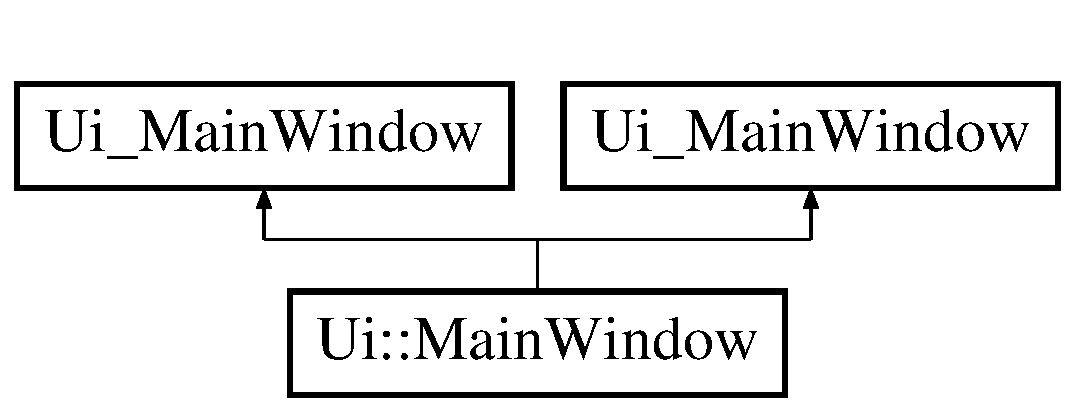
\includegraphics[height=2.000000cm]{d9/dbd/classUi_1_1MainWindow}
\end{center}
\end{figure}
\subsection*{Dodatkowe Dziedziczone Składowe}


Dokumentacja dla tej klasy została wygenerowana z pliku\-:\begin{DoxyCompactItemize}
\item 
Gra\-Figury/\hyperlink{GraFigury_2ui__mainwindow_8h}{ui\-\_\-mainwindow.\-h}\end{DoxyCompactItemize}

\hypertarget{classMainWindow}{\section{Dokumentacja klasy Main\-Window}
\label{classMainWindow}\index{Main\-Window@{Main\-Window}}
}


{\ttfamily \#include $<$mainwindow.\-h$>$}

Diagram dziedziczenia dla Main\-Window\begin{figure}[H]
\begin{center}
\leavevmode
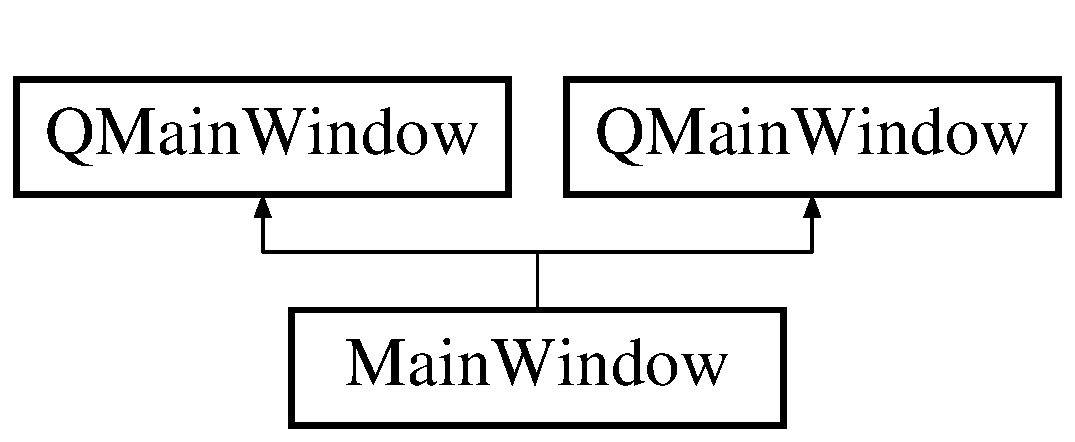
\includegraphics[height=2.000000cm]{d6/d1a/classMainWindow}
\end{center}
\end{figure}
\subsection*{Typy publiczne}
\begin{DoxyCompactItemize}
\item 
enum \{ \hyperlink{classMainWindow_ac0baac8464ccf6e6ea7e8f21f18484ffa67c2ad1aed243f6be7a551108477d9e0}{F\-I\-G\-U\-R\-Y}, 
\hyperlink{classMainWindow_ac0baac8464ccf6e6ea7e8f21f18484ffa642a5a52542d22e67554f60eda6e541d}{I\-N\-F\-O}
 \}
\end{DoxyCompactItemize}
\subsection*{Sygnały}
\begin{DoxyCompactItemize}
\item 
void \hyperlink{classMainWindow_a5375b14904048c4f5c258183999afbf3}{usun\-Figury\-Signal} ()
\end{DoxyCompactItemize}
\subsection*{Metody publiczne}
\begin{DoxyCompactItemize}
\item 
\hyperlink{classMainWindow_a8b244be8b7b7db1b08de2a2acb9409db}{Main\-Window} (Q\-Widget $\ast$parent=0)
\item 
\hyperlink{classMainWindow_ae98d00a93bc118200eeef9f9bba1dba7}{$\sim$\-Main\-Window} ()
\item 
\hyperlink{classMainWindow_a8b244be8b7b7db1b08de2a2acb9409db}{Main\-Window} (Q\-Widget $\ast$parent=0)
\item 
\hyperlink{classMainWindow_ae98d00a93bc118200eeef9f9bba1dba7}{$\sim$\-Main\-Window} ()
\end{DoxyCompactItemize}
\subsection*{Sloty prywatne}
\begin{DoxyCompactItemize}
\item 
void \hyperlink{classMainWindow_aeef45c5364f5d7843a260b01cf94f22e}{connect\-To\-Server} (Q\-String, int)
\item 
void \hyperlink{classMainWindow_ae426c78e710d74fa6cc67b0d73ade293}{new\-Message} ()
\item 
void \hyperlink{classMainWindow_a2d0da471c4fe51fc90f1079d856db068}{on\-\_\-push\-Button\-Polacz\-\_\-clicked} ()
\item 
void \hyperlink{classMainWindow_a6b8e934fca603cf7678eabb9a6dfc709}{key\-Press\-Event} (Q\-Key\-Event $\ast$)
\item 
void \hyperlink{classMainWindow_a47b54ea4678d72f712370f550634dfac}{zmien\-Poziom\-Message} ()
\item 
void \hyperlink{classMainWindow_a9abc4d8b5fac6ef7ad91ccd1181b21a8}{open\-Session} ()
\item 
void \hyperlink{classMainWindow_ade49de88616301ebc06e28993164a183}{new\-Connection} ()
\item 
void \hyperlink{classMainWindow_ae426c78e710d74fa6cc67b0d73ade293}{new\-Message} ()
\item 
void \hyperlink{classMainWindow_aef52274d67fbe13062dafd43e27529cb}{on\-\_\-timer} ()
\item 
void \hyperlink{classMainWindow_aa4f477acccb935dc77109944c036c66e}{client\-Disconnected} ()
\item 
void \hyperlink{classMainWindow_a7a57f41cd36b4221181dc661a69954bf}{on\-\_\-push\-Button\-Start\-\_\-clicked} ()
\item 
void \hyperlink{classMainWindow_a95ec84452d77bf97d2a16f3d9c6ea8b8}{on\-\_\-push\-Button\-Stop\-\_\-clicked} ()
\end{DoxyCompactItemize}
\subsection*{Metody prywatne}
\begin{DoxyCompactItemize}
\item 
void \hyperlink{classMainWindow_a2d51371a2ba5783e209e4973d66968a9}{zmien\-Poziom} (int i)
\item 
void \hyperlink{classMainWindow_a28c4dda2a0ac0872677bcd088ec10258}{koniec\-Poziomu} (int)
\item 
void \hyperlink{classMainWindow_a817826befb881a9136a1d76dc64f8a67}{ruch\-Odrzutowy} (int, int)
\item 
void \hyperlink{classMainWindow_a8217ee19e4707d2ceea1ca62521806b7}{ruch\-Figur} ()
\item 
void \hyperlink{classMainWindow_a6c5e5435014fa2b8b1a30e3d5375f6af}{zjadanie\-Mniejszych} ()
\item 
void \hyperlink{classMainWindow_a3cf5b16f1c7da3d94cfb61fb8925871e}{usun\-Odicnki} ()
\item 
void \hyperlink{classMainWindow_af892d930f6529eb2831d5b05634a1dab}{usun\-Figury} ()
\end{DoxyCompactItemize}
\subsection*{Atrybuty prywatne}
\begin{DoxyCompactItemize}
\item 
Q\-List$<$ \hyperlink{classFigura}{Figura} $\ast$ $>$ \hyperlink{classMainWindow_a8a91987c12db69417cdb275cf712b9df}{lista\-Figur}
\item 
Q\-List$<$ \hyperlink{classOdcinek}{Odcinek} $\ast$ $>$ \hyperlink{classMainWindow_abaa648f21383f580a833d7ed90f75926}{lista\-Odcinkow}
\item 
\hyperlink{classUi_1_1MainWindow}{Ui\-::\-Main\-Window} $\ast$ \hyperlink{classMainWindow_a43606649aeaf9e561328935fca0cd1bf}{ui}
\item 
Q\-Tcp\-Socket $\ast$ \hyperlink{classMainWindow_af85cfe62c116f8d2f2021e5411b0356e}{socket}
\item 
\hyperlink{classDialog}{Dialog} $\ast$ \hyperlink{classMainWindow_a029f5f35facf7120bbf42e54dbd25a40}{dialog}
\item 
\hyperlink{classDialog2}{Dialog2} $\ast$ \hyperlink{classMainWindow_acca874ff840ec87fe90e0acc72d40e5a}{dialog2}
\item 
int \hyperlink{classMainWindow_a2b0740aaca0b5b566008e55916d4d0e9}{wynik}
\item 
Q\-Tcp\-Server $\ast$ \hyperlink{classMainWindow_a4b1e890b4b33f6ff8c22621d2ce55c2d}{server}
\item 
Q\-Network\-Session $\ast$ \hyperlink{classMainWindow_a638a10aec0de799787205387ee4da83e}{network\-Session}
\item 
Q\-List$<$ Q\-Tcp\-Socket $\ast$ $>$ \hyperlink{classMainWindow_a698f52eb8759a1cde60c5638670b078e}{clients}
\item 
int \hyperlink{classMainWindow_a0909fe6df1d60edacad5591acb011a2f}{ramka\-Przyblizania}
\item 
G\-Lfloat \hyperlink{classMainWindow_a8e9fb49dd7c36fac9e2d83b555e0caa6}{tlo} \mbox{[}4\mbox{]}
\item 
\hyperlink{classPoziomy}{Poziomy} \hyperlink{classMainWindow_a6bc6d2f12427573392ddfbc8d7f454fd}{poziomy}
\item 
Q\-Point\-F \hyperlink{classMainWindow_a479094513b0598030f63a24963e2109e}{last\-Pos}
\item 
Q\-Timer \hyperlink{classMainWindow_a3c80cf51d9dfb16e655a7e25f8016e3b}{timer}
\item 
int \hyperlink{classMainWindow_a0fae41d96da5ca0d54f398025e19ec3a}{Ts}
\item 
int \hyperlink{classMainWindow_aeff57fcdb7d82d6f69b1214ce24d1ecd}{aktualny\-Poziom}
\item 
bool \hyperlink{classMainWindow_a331bf910d34ef19115989bba99c16b7b}{zmiana}
\item 
bool \hyperlink{classMainWindow_a071cbb3e764cd5a0d37033a5eb82b1e0}{wyslano\-Koniec\-Poziomu}
\end{DoxyCompactItemize}


\subsection{Dokumentacja składowych wyliczanych}
\hypertarget{classMainWindow_ac0baac8464ccf6e6ea7e8f21f18484ff}{\subsubsection[{anonymous enum}]{\setlength{\rightskip}{0pt plus 5cm}anonymous enum}}\label{classMainWindow_ac0baac8464ccf6e6ea7e8f21f18484ff}
\begin{Desc}
\item[Wartości wyliczeń]\par
\begin{description}
\index{F\-I\-G\-U\-R\-Y@{F\-I\-G\-U\-R\-Y}!Main\-Window@{Main\-Window}}\index{Main\-Window@{Main\-Window}!F\-I\-G\-U\-R\-Y@{F\-I\-G\-U\-R\-Y}}\item[{\em 
\hypertarget{classMainWindow_ac0baac8464ccf6e6ea7e8f21f18484ffa67c2ad1aed243f6be7a551108477d9e0}{F\-I\-G\-U\-R\-Y}\label{classMainWindow_ac0baac8464ccf6e6ea7e8f21f18484ffa67c2ad1aed243f6be7a551108477d9e0}
}]\index{I\-N\-F\-O@{I\-N\-F\-O}!Main\-Window@{Main\-Window}}\index{Main\-Window@{Main\-Window}!I\-N\-F\-O@{I\-N\-F\-O}}\item[{\em 
\hypertarget{classMainWindow_ac0baac8464ccf6e6ea7e8f21f18484ffa642a5a52542d22e67554f60eda6e541d}{I\-N\-F\-O}\label{classMainWindow_ac0baac8464ccf6e6ea7e8f21f18484ffa642a5a52542d22e67554f60eda6e541d}
}]\end{description}
\end{Desc}


\subsection{Dokumentacja konstruktora i destruktora}
\hypertarget{classMainWindow_a8b244be8b7b7db1b08de2a2acb9409db}{\index{Main\-Window@{Main\-Window}!Main\-Window@{Main\-Window}}
\index{Main\-Window@{Main\-Window}!MainWindow@{Main\-Window}}
\subsubsection[{Main\-Window}]{\setlength{\rightskip}{0pt plus 5cm}Main\-Window\-::\-Main\-Window (
\begin{DoxyParamCaption}
\item[{Q\-Widget $\ast$}]{parent = {\ttfamily 0}}
\end{DoxyParamCaption}
)\hspace{0.3cm}{\ttfamily [explicit]}}}\label{classMainWindow_a8b244be8b7b7db1b08de2a2acb9409db}
\hypertarget{classMainWindow_ae98d00a93bc118200eeef9f9bba1dba7}{\index{Main\-Window@{Main\-Window}!$\sim$\-Main\-Window@{$\sim$\-Main\-Window}}
\index{$\sim$\-Main\-Window@{$\sim$\-Main\-Window}!MainWindow@{Main\-Window}}
\subsubsection[{$\sim$\-Main\-Window}]{\setlength{\rightskip}{0pt plus 5cm}Main\-Window\-::$\sim$\-Main\-Window (
\begin{DoxyParamCaption}
{}
\end{DoxyParamCaption}
)}}\label{classMainWindow_ae98d00a93bc118200eeef9f9bba1dba7}
\hypertarget{classMainWindow_a8b244be8b7b7db1b08de2a2acb9409db}{\index{Main\-Window@{Main\-Window}!Main\-Window@{Main\-Window}}
\index{Main\-Window@{Main\-Window}!MainWindow@{Main\-Window}}
\subsubsection[{Main\-Window}]{\setlength{\rightskip}{0pt plus 5cm}Main\-Window\-::\-Main\-Window (
\begin{DoxyParamCaption}
\item[{Q\-Widget $\ast$}]{parent = {\ttfamily 0}}
\end{DoxyParamCaption}
)\hspace{0.3cm}{\ttfamily [explicit]}}}\label{classMainWindow_a8b244be8b7b7db1b08de2a2acb9409db}
\hypertarget{classMainWindow_ae98d00a93bc118200eeef9f9bba1dba7}{\index{Main\-Window@{Main\-Window}!$\sim$\-Main\-Window@{$\sim$\-Main\-Window}}
\index{$\sim$\-Main\-Window@{$\sim$\-Main\-Window}!MainWindow@{Main\-Window}}
\subsubsection[{$\sim$\-Main\-Window}]{\setlength{\rightskip}{0pt plus 5cm}Main\-Window\-::$\sim$\-Main\-Window (
\begin{DoxyParamCaption}
{}
\end{DoxyParamCaption}
)}}\label{classMainWindow_ae98d00a93bc118200eeef9f9bba1dba7}


\subsection{Dokumentacja funkcji składowych}
\hypertarget{classMainWindow_aa4f477acccb935dc77109944c036c66e}{\index{Main\-Window@{Main\-Window}!client\-Disconnected@{client\-Disconnected}}
\index{client\-Disconnected@{client\-Disconnected}!MainWindow@{Main\-Window}}
\subsubsection[{client\-Disconnected}]{\setlength{\rightskip}{0pt plus 5cm}void Main\-Window\-::client\-Disconnected (
\begin{DoxyParamCaption}
{}
\end{DoxyParamCaption}
)\hspace{0.3cm}{\ttfamily [private]}, {\ttfamily [slot]}}}\label{classMainWindow_aa4f477acccb935dc77109944c036c66e}
\hypertarget{classMainWindow_aeef45c5364f5d7843a260b01cf94f22e}{\index{Main\-Window@{Main\-Window}!connect\-To\-Server@{connect\-To\-Server}}
\index{connect\-To\-Server@{connect\-To\-Server}!MainWindow@{Main\-Window}}
\subsubsection[{connect\-To\-Server}]{\setlength{\rightskip}{0pt plus 5cm}void Main\-Window\-::connect\-To\-Server (
\begin{DoxyParamCaption}
\item[{Q\-String}]{ip, }
\item[{int}]{port}
\end{DoxyParamCaption}
)\hspace{0.3cm}{\ttfamily [private]}, {\ttfamily [slot]}}}\label{classMainWindow_aeef45c5364f5d7843a260b01cf94f22e}
\hypertarget{classMainWindow_a6b8e934fca603cf7678eabb9a6dfc709}{\index{Main\-Window@{Main\-Window}!key\-Press\-Event@{key\-Press\-Event}}
\index{key\-Press\-Event@{key\-Press\-Event}!MainWindow@{Main\-Window}}
\subsubsection[{key\-Press\-Event}]{\setlength{\rightskip}{0pt plus 5cm}void Main\-Window\-::key\-Press\-Event (
\begin{DoxyParamCaption}
\item[{Q\-Key\-Event $\ast$}]{event}
\end{DoxyParamCaption}
)\hspace{0.3cm}{\ttfamily [private]}, {\ttfamily [slot]}}}\label{classMainWindow_a6b8e934fca603cf7678eabb9a6dfc709}
\hypertarget{classMainWindow_a28c4dda2a0ac0872677bcd088ec10258}{\index{Main\-Window@{Main\-Window}!koniec\-Poziomu@{koniec\-Poziomu}}
\index{koniec\-Poziomu@{koniec\-Poziomu}!MainWindow@{Main\-Window}}
\subsubsection[{koniec\-Poziomu}]{\setlength{\rightskip}{0pt plus 5cm}void Main\-Window\-::koniec\-Poziomu (
\begin{DoxyParamCaption}
\item[{int}]{gracz\-Aktywny}
\end{DoxyParamCaption}
)\hspace{0.3cm}{\ttfamily [private]}}}\label{classMainWindow_a28c4dda2a0ac0872677bcd088ec10258}
\hypertarget{classMainWindow_ade49de88616301ebc06e28993164a183}{\index{Main\-Window@{Main\-Window}!new\-Connection@{new\-Connection}}
\index{new\-Connection@{new\-Connection}!MainWindow@{Main\-Window}}
\subsubsection[{new\-Connection}]{\setlength{\rightskip}{0pt plus 5cm}void Main\-Window\-::new\-Connection (
\begin{DoxyParamCaption}
{}
\end{DoxyParamCaption}
)\hspace{0.3cm}{\ttfamily [private]}, {\ttfamily [slot]}}}\label{classMainWindow_ade49de88616301ebc06e28993164a183}
\hypertarget{classMainWindow_ae426c78e710d74fa6cc67b0d73ade293}{\index{Main\-Window@{Main\-Window}!new\-Message@{new\-Message}}
\index{new\-Message@{new\-Message}!MainWindow@{Main\-Window}}
\subsubsection[{new\-Message}]{\setlength{\rightskip}{0pt plus 5cm}void Main\-Window\-::new\-Message (
\begin{DoxyParamCaption}
{}
\end{DoxyParamCaption}
)\hspace{0.3cm}{\ttfamily [private]}, {\ttfamily [slot]}}}\label{classMainWindow_ae426c78e710d74fa6cc67b0d73ade293}
\hypertarget{classMainWindow_ae426c78e710d74fa6cc67b0d73ade293}{\index{Main\-Window@{Main\-Window}!new\-Message@{new\-Message}}
\index{new\-Message@{new\-Message}!MainWindow@{Main\-Window}}
\subsubsection[{new\-Message}]{\setlength{\rightskip}{0pt plus 5cm}void Main\-Window\-::new\-Message (
\begin{DoxyParamCaption}
{}
\end{DoxyParamCaption}
)\hspace{0.3cm}{\ttfamily [private]}, {\ttfamily [slot]}}}\label{classMainWindow_ae426c78e710d74fa6cc67b0d73ade293}
\hypertarget{classMainWindow_a2d0da471c4fe51fc90f1079d856db068}{\index{Main\-Window@{Main\-Window}!on\-\_\-push\-Button\-Polacz\-\_\-clicked@{on\-\_\-push\-Button\-Polacz\-\_\-clicked}}
\index{on\-\_\-push\-Button\-Polacz\-\_\-clicked@{on\-\_\-push\-Button\-Polacz\-\_\-clicked}!MainWindow@{Main\-Window}}
\subsubsection[{on\-\_\-push\-Button\-Polacz\-\_\-clicked}]{\setlength{\rightskip}{0pt plus 5cm}void Main\-Window\-::on\-\_\-push\-Button\-Polacz\-\_\-clicked (
\begin{DoxyParamCaption}
{}
\end{DoxyParamCaption}
)\hspace{0.3cm}{\ttfamily [private]}, {\ttfamily [slot]}}}\label{classMainWindow_a2d0da471c4fe51fc90f1079d856db068}
\hypertarget{classMainWindow_a7a57f41cd36b4221181dc661a69954bf}{\index{Main\-Window@{Main\-Window}!on\-\_\-push\-Button\-Start\-\_\-clicked@{on\-\_\-push\-Button\-Start\-\_\-clicked}}
\index{on\-\_\-push\-Button\-Start\-\_\-clicked@{on\-\_\-push\-Button\-Start\-\_\-clicked}!MainWindow@{Main\-Window}}
\subsubsection[{on\-\_\-push\-Button\-Start\-\_\-clicked}]{\setlength{\rightskip}{0pt plus 5cm}void Main\-Window\-::on\-\_\-push\-Button\-Start\-\_\-clicked (
\begin{DoxyParamCaption}
{}
\end{DoxyParamCaption}
)\hspace{0.3cm}{\ttfamily [private]}, {\ttfamily [slot]}}}\label{classMainWindow_a7a57f41cd36b4221181dc661a69954bf}
\hypertarget{classMainWindow_a95ec84452d77bf97d2a16f3d9c6ea8b8}{\index{Main\-Window@{Main\-Window}!on\-\_\-push\-Button\-Stop\-\_\-clicked@{on\-\_\-push\-Button\-Stop\-\_\-clicked}}
\index{on\-\_\-push\-Button\-Stop\-\_\-clicked@{on\-\_\-push\-Button\-Stop\-\_\-clicked}!MainWindow@{Main\-Window}}
\subsubsection[{on\-\_\-push\-Button\-Stop\-\_\-clicked}]{\setlength{\rightskip}{0pt plus 5cm}void Main\-Window\-::on\-\_\-push\-Button\-Stop\-\_\-clicked (
\begin{DoxyParamCaption}
{}
\end{DoxyParamCaption}
)\hspace{0.3cm}{\ttfamily [private]}, {\ttfamily [slot]}}}\label{classMainWindow_a95ec84452d77bf97d2a16f3d9c6ea8b8}
\hypertarget{classMainWindow_aef52274d67fbe13062dafd43e27529cb}{\index{Main\-Window@{Main\-Window}!on\-\_\-timer@{on\-\_\-timer}}
\index{on\-\_\-timer@{on\-\_\-timer}!MainWindow@{Main\-Window}}
\subsubsection[{on\-\_\-timer}]{\setlength{\rightskip}{0pt plus 5cm}void Main\-Window\-::on\-\_\-timer (
\begin{DoxyParamCaption}
{}
\end{DoxyParamCaption}
)\hspace{0.3cm}{\ttfamily [private]}, {\ttfamily [slot]}}}\label{classMainWindow_aef52274d67fbe13062dafd43e27529cb}
\hypertarget{classMainWindow_a9abc4d8b5fac6ef7ad91ccd1181b21a8}{\index{Main\-Window@{Main\-Window}!open\-Session@{open\-Session}}
\index{open\-Session@{open\-Session}!MainWindow@{Main\-Window}}
\subsubsection[{open\-Session}]{\setlength{\rightskip}{0pt plus 5cm}void Main\-Window\-::open\-Session (
\begin{DoxyParamCaption}
{}
\end{DoxyParamCaption}
)\hspace{0.3cm}{\ttfamily [private]}, {\ttfamily [slot]}}}\label{classMainWindow_a9abc4d8b5fac6ef7ad91ccd1181b21a8}
\hypertarget{classMainWindow_a8217ee19e4707d2ceea1ca62521806b7}{\index{Main\-Window@{Main\-Window}!ruch\-Figur@{ruch\-Figur}}
\index{ruch\-Figur@{ruch\-Figur}!MainWindow@{Main\-Window}}
\subsubsection[{ruch\-Figur}]{\setlength{\rightskip}{0pt plus 5cm}void Main\-Window\-::ruch\-Figur (
\begin{DoxyParamCaption}
{}
\end{DoxyParamCaption}
)\hspace{0.3cm}{\ttfamily [private]}}}\label{classMainWindow_a8217ee19e4707d2ceea1ca62521806b7}
\hypertarget{classMainWindow_a817826befb881a9136a1d76dc64f8a67}{\index{Main\-Window@{Main\-Window}!ruch\-Odrzutowy@{ruch\-Odrzutowy}}
\index{ruch\-Odrzutowy@{ruch\-Odrzutowy}!MainWindow@{Main\-Window}}
\subsubsection[{ruch\-Odrzutowy}]{\setlength{\rightskip}{0pt plus 5cm}void Main\-Window\-::ruch\-Odrzutowy (
\begin{DoxyParamCaption}
\item[{int}]{key, }
\item[{int}]{i}
\end{DoxyParamCaption}
)\hspace{0.3cm}{\ttfamily [private]}}}\label{classMainWindow_a817826befb881a9136a1d76dc64f8a67}
\hypertarget{classMainWindow_af892d930f6529eb2831d5b05634a1dab}{\index{Main\-Window@{Main\-Window}!usun\-Figury@{usun\-Figury}}
\index{usun\-Figury@{usun\-Figury}!MainWindow@{Main\-Window}}
\subsubsection[{usun\-Figury}]{\setlength{\rightskip}{0pt plus 5cm}void Main\-Window\-::usun\-Figury (
\begin{DoxyParamCaption}
{}
\end{DoxyParamCaption}
)\hspace{0.3cm}{\ttfamily [private]}}}\label{classMainWindow_af892d930f6529eb2831d5b05634a1dab}
\hypertarget{classMainWindow_a5375b14904048c4f5c258183999afbf3}{\index{Main\-Window@{Main\-Window}!usun\-Figury\-Signal@{usun\-Figury\-Signal}}
\index{usun\-Figury\-Signal@{usun\-Figury\-Signal}!MainWindow@{Main\-Window}}
\subsubsection[{usun\-Figury\-Signal}]{\setlength{\rightskip}{0pt plus 5cm}void Main\-Window\-::usun\-Figury\-Signal (
\begin{DoxyParamCaption}
{}
\end{DoxyParamCaption}
)\hspace{0.3cm}{\ttfamily [signal]}}}\label{classMainWindow_a5375b14904048c4f5c258183999afbf3}
\hypertarget{classMainWindow_a3cf5b16f1c7da3d94cfb61fb8925871e}{\index{Main\-Window@{Main\-Window}!usun\-Odicnki@{usun\-Odicnki}}
\index{usun\-Odicnki@{usun\-Odicnki}!MainWindow@{Main\-Window}}
\subsubsection[{usun\-Odicnki}]{\setlength{\rightskip}{0pt plus 5cm}void Main\-Window\-::usun\-Odicnki (
\begin{DoxyParamCaption}
{}
\end{DoxyParamCaption}
)\hspace{0.3cm}{\ttfamily [private]}}}\label{classMainWindow_a3cf5b16f1c7da3d94cfb61fb8925871e}
\hypertarget{classMainWindow_a6c5e5435014fa2b8b1a30e3d5375f6af}{\index{Main\-Window@{Main\-Window}!zjadanie\-Mniejszych@{zjadanie\-Mniejszych}}
\index{zjadanie\-Mniejszych@{zjadanie\-Mniejszych}!MainWindow@{Main\-Window}}
\subsubsection[{zjadanie\-Mniejszych}]{\setlength{\rightskip}{0pt plus 5cm}void Main\-Window\-::zjadanie\-Mniejszych (
\begin{DoxyParamCaption}
{}
\end{DoxyParamCaption}
)\hspace{0.3cm}{\ttfamily [private]}}}\label{classMainWindow_a6c5e5435014fa2b8b1a30e3d5375f6af}
\hypertarget{classMainWindow_a2d51371a2ba5783e209e4973d66968a9}{\index{Main\-Window@{Main\-Window}!zmien\-Poziom@{zmien\-Poziom}}
\index{zmien\-Poziom@{zmien\-Poziom}!MainWindow@{Main\-Window}}
\subsubsection[{zmien\-Poziom}]{\setlength{\rightskip}{0pt plus 5cm}void Main\-Window\-::zmien\-Poziom (
\begin{DoxyParamCaption}
\item[{int}]{i}
\end{DoxyParamCaption}
)\hspace{0.3cm}{\ttfamily [private]}}}\label{classMainWindow_a2d51371a2ba5783e209e4973d66968a9}
\hypertarget{classMainWindow_a47b54ea4678d72f712370f550634dfac}{\index{Main\-Window@{Main\-Window}!zmien\-Poziom\-Message@{zmien\-Poziom\-Message}}
\index{zmien\-Poziom\-Message@{zmien\-Poziom\-Message}!MainWindow@{Main\-Window}}
\subsubsection[{zmien\-Poziom\-Message}]{\setlength{\rightskip}{0pt plus 5cm}void Main\-Window\-::zmien\-Poziom\-Message (
\begin{DoxyParamCaption}
{}
\end{DoxyParamCaption}
)\hspace{0.3cm}{\ttfamily [private]}, {\ttfamily [slot]}}}\label{classMainWindow_a47b54ea4678d72f712370f550634dfac}


\subsection{Dokumentacja atrybutów składowych}
\hypertarget{classMainWindow_aeff57fcdb7d82d6f69b1214ce24d1ecd}{\index{Main\-Window@{Main\-Window}!aktualny\-Poziom@{aktualny\-Poziom}}
\index{aktualny\-Poziom@{aktualny\-Poziom}!MainWindow@{Main\-Window}}
\subsubsection[{aktualny\-Poziom}]{\setlength{\rightskip}{0pt plus 5cm}int Main\-Window\-::aktualny\-Poziom\hspace{0.3cm}{\ttfamily [private]}}}\label{classMainWindow_aeff57fcdb7d82d6f69b1214ce24d1ecd}
\hypertarget{classMainWindow_a698f52eb8759a1cde60c5638670b078e}{\index{Main\-Window@{Main\-Window}!clients@{clients}}
\index{clients@{clients}!MainWindow@{Main\-Window}}
\subsubsection[{clients}]{\setlength{\rightskip}{0pt plus 5cm}Q\-List$<$Q\-Tcp\-Socket$\ast$$>$ Main\-Window\-::clients\hspace{0.3cm}{\ttfamily [private]}}}\label{classMainWindow_a698f52eb8759a1cde60c5638670b078e}
\hypertarget{classMainWindow_a029f5f35facf7120bbf42e54dbd25a40}{\index{Main\-Window@{Main\-Window}!dialog@{dialog}}
\index{dialog@{dialog}!MainWindow@{Main\-Window}}
\subsubsection[{dialog}]{\setlength{\rightskip}{0pt plus 5cm}{\bf Dialog}$\ast$ Main\-Window\-::dialog\hspace{0.3cm}{\ttfamily [private]}}}\label{classMainWindow_a029f5f35facf7120bbf42e54dbd25a40}
\hypertarget{classMainWindow_acca874ff840ec87fe90e0acc72d40e5a}{\index{Main\-Window@{Main\-Window}!dialog2@{dialog2}}
\index{dialog2@{dialog2}!MainWindow@{Main\-Window}}
\subsubsection[{dialog2}]{\setlength{\rightskip}{0pt plus 5cm}{\bf Dialog2}$\ast$ Main\-Window\-::dialog2\hspace{0.3cm}{\ttfamily [private]}}}\label{classMainWindow_acca874ff840ec87fe90e0acc72d40e5a}
\hypertarget{classMainWindow_a479094513b0598030f63a24963e2109e}{\index{Main\-Window@{Main\-Window}!last\-Pos@{last\-Pos}}
\index{last\-Pos@{last\-Pos}!MainWindow@{Main\-Window}}
\subsubsection[{last\-Pos}]{\setlength{\rightskip}{0pt plus 5cm}Q\-Point\-F Main\-Window\-::last\-Pos\hspace{0.3cm}{\ttfamily [private]}}}\label{classMainWindow_a479094513b0598030f63a24963e2109e}
\hypertarget{classMainWindow_a8a91987c12db69417cdb275cf712b9df}{\index{Main\-Window@{Main\-Window}!lista\-Figur@{lista\-Figur}}
\index{lista\-Figur@{lista\-Figur}!MainWindow@{Main\-Window}}
\subsubsection[{lista\-Figur}]{\setlength{\rightskip}{0pt plus 5cm}Q\-List$<$ {\bf Figura} $\ast$ $>$ Main\-Window\-::lista\-Figur\hspace{0.3cm}{\ttfamily [private]}}}\label{classMainWindow_a8a91987c12db69417cdb275cf712b9df}
\hypertarget{classMainWindow_abaa648f21383f580a833d7ed90f75926}{\index{Main\-Window@{Main\-Window}!lista\-Odcinkow@{lista\-Odcinkow}}
\index{lista\-Odcinkow@{lista\-Odcinkow}!MainWindow@{Main\-Window}}
\subsubsection[{lista\-Odcinkow}]{\setlength{\rightskip}{0pt plus 5cm}Q\-List$<$ {\bf Odcinek} $\ast$ $>$ Main\-Window\-::lista\-Odcinkow\hspace{0.3cm}{\ttfamily [private]}}}\label{classMainWindow_abaa648f21383f580a833d7ed90f75926}
\hypertarget{classMainWindow_a638a10aec0de799787205387ee4da83e}{\index{Main\-Window@{Main\-Window}!network\-Session@{network\-Session}}
\index{network\-Session@{network\-Session}!MainWindow@{Main\-Window}}
\subsubsection[{network\-Session}]{\setlength{\rightskip}{0pt plus 5cm}Q\-Network\-Session$\ast$ Main\-Window\-::network\-Session\hspace{0.3cm}{\ttfamily [private]}}}\label{classMainWindow_a638a10aec0de799787205387ee4da83e}
\hypertarget{classMainWindow_a6bc6d2f12427573392ddfbc8d7f454fd}{\index{Main\-Window@{Main\-Window}!poziomy@{poziomy}}
\index{poziomy@{poziomy}!MainWindow@{Main\-Window}}
\subsubsection[{poziomy}]{\setlength{\rightskip}{0pt plus 5cm}{\bf Poziomy} Main\-Window\-::poziomy\hspace{0.3cm}{\ttfamily [private]}}}\label{classMainWindow_a6bc6d2f12427573392ddfbc8d7f454fd}
\hypertarget{classMainWindow_a0909fe6df1d60edacad5591acb011a2f}{\index{Main\-Window@{Main\-Window}!ramka\-Przyblizania@{ramka\-Przyblizania}}
\index{ramka\-Przyblizania@{ramka\-Przyblizania}!MainWindow@{Main\-Window}}
\subsubsection[{ramka\-Przyblizania}]{\setlength{\rightskip}{0pt plus 5cm}int Main\-Window\-::ramka\-Przyblizania\hspace{0.3cm}{\ttfamily [private]}}}\label{classMainWindow_a0909fe6df1d60edacad5591acb011a2f}
\hypertarget{classMainWindow_a4b1e890b4b33f6ff8c22621d2ce55c2d}{\index{Main\-Window@{Main\-Window}!server@{server}}
\index{server@{server}!MainWindow@{Main\-Window}}
\subsubsection[{server}]{\setlength{\rightskip}{0pt plus 5cm}Q\-Tcp\-Server$\ast$ Main\-Window\-::server\hspace{0.3cm}{\ttfamily [private]}}}\label{classMainWindow_a4b1e890b4b33f6ff8c22621d2ce55c2d}
\hypertarget{classMainWindow_af85cfe62c116f8d2f2021e5411b0356e}{\index{Main\-Window@{Main\-Window}!socket@{socket}}
\index{socket@{socket}!MainWindow@{Main\-Window}}
\subsubsection[{socket}]{\setlength{\rightskip}{0pt plus 5cm}Q\-Tcp\-Socket$\ast$ Main\-Window\-::socket\hspace{0.3cm}{\ttfamily [private]}}}\label{classMainWindow_af85cfe62c116f8d2f2021e5411b0356e}
\hypertarget{classMainWindow_a3c80cf51d9dfb16e655a7e25f8016e3b}{\index{Main\-Window@{Main\-Window}!timer@{timer}}
\index{timer@{timer}!MainWindow@{Main\-Window}}
\subsubsection[{timer}]{\setlength{\rightskip}{0pt plus 5cm}Q\-Timer Main\-Window\-::timer\hspace{0.3cm}{\ttfamily [private]}}}\label{classMainWindow_a3c80cf51d9dfb16e655a7e25f8016e3b}
\hypertarget{classMainWindow_a8e9fb49dd7c36fac9e2d83b555e0caa6}{\index{Main\-Window@{Main\-Window}!tlo@{tlo}}
\index{tlo@{tlo}!MainWindow@{Main\-Window}}
\subsubsection[{tlo}]{\setlength{\rightskip}{0pt plus 5cm}G\-Lfloat Main\-Window\-::tlo\mbox{[}4\mbox{]}\hspace{0.3cm}{\ttfamily [private]}}}\label{classMainWindow_a8e9fb49dd7c36fac9e2d83b555e0caa6}
\hypertarget{classMainWindow_a0fae41d96da5ca0d54f398025e19ec3a}{\index{Main\-Window@{Main\-Window}!Ts@{Ts}}
\index{Ts@{Ts}!MainWindow@{Main\-Window}}
\subsubsection[{Ts}]{\setlength{\rightskip}{0pt plus 5cm}int Main\-Window\-::\-Ts\hspace{0.3cm}{\ttfamily [private]}}}\label{classMainWindow_a0fae41d96da5ca0d54f398025e19ec3a}
\hypertarget{classMainWindow_a43606649aeaf9e561328935fca0cd1bf}{\index{Main\-Window@{Main\-Window}!ui@{ui}}
\index{ui@{ui}!MainWindow@{Main\-Window}}
\subsubsection[{ui}]{\setlength{\rightskip}{0pt plus 5cm}{\bf Ui\-::\-Main\-Window} $\ast$ Main\-Window\-::ui\hspace{0.3cm}{\ttfamily [private]}}}\label{classMainWindow_a43606649aeaf9e561328935fca0cd1bf}
\hypertarget{classMainWindow_a2b0740aaca0b5b566008e55916d4d0e9}{\index{Main\-Window@{Main\-Window}!wynik@{wynik}}
\index{wynik@{wynik}!MainWindow@{Main\-Window}}
\subsubsection[{wynik}]{\setlength{\rightskip}{0pt plus 5cm}int Main\-Window\-::wynik\hspace{0.3cm}{\ttfamily [private]}}}\label{classMainWindow_a2b0740aaca0b5b566008e55916d4d0e9}
\hypertarget{classMainWindow_a071cbb3e764cd5a0d37033a5eb82b1e0}{\index{Main\-Window@{Main\-Window}!wyslano\-Koniec\-Poziomu@{wyslano\-Koniec\-Poziomu}}
\index{wyslano\-Koniec\-Poziomu@{wyslano\-Koniec\-Poziomu}!MainWindow@{Main\-Window}}
\subsubsection[{wyslano\-Koniec\-Poziomu}]{\setlength{\rightskip}{0pt plus 5cm}bool Main\-Window\-::wyslano\-Koniec\-Poziomu\hspace{0.3cm}{\ttfamily [private]}}}\label{classMainWindow_a071cbb3e764cd5a0d37033a5eb82b1e0}
\hypertarget{classMainWindow_a331bf910d34ef19115989bba99c16b7b}{\index{Main\-Window@{Main\-Window}!zmiana@{zmiana}}
\index{zmiana@{zmiana}!MainWindow@{Main\-Window}}
\subsubsection[{zmiana}]{\setlength{\rightskip}{0pt plus 5cm}bool Main\-Window\-::zmiana\hspace{0.3cm}{\ttfamily [private]}}}\label{classMainWindow_a331bf910d34ef19115989bba99c16b7b}


Dokumentacja dla tej klasy została wygenerowana z plików\-:\begin{DoxyCompactItemize}
\item 
Gra\-Figury/\hyperlink{GraFigury_2mainwindow_8h}{mainwindow.\-h}\item 
Gra\-Figury/\hyperlink{GraFigury_2mainwindow_8cpp}{mainwindow.\-cpp}\item 
Serwer\-Figury/\hyperlink{SerwerFigury_2moc__mainwindow_8cpp}{moc\-\_\-mainwindow.\-cpp}\end{DoxyCompactItemize}

\hypertarget{classMyGLWidget}{\section{Dokumentacja klasy My\-G\-L\-Widget}
\label{classMyGLWidget}\index{My\-G\-L\-Widget@{My\-G\-L\-Widget}}
}


{\ttfamily \#include $<$myglwidget.\-h$>$}

Diagram dziedziczenia dla My\-G\-L\-Widget\begin{figure}[H]
\begin{center}
\leavevmode
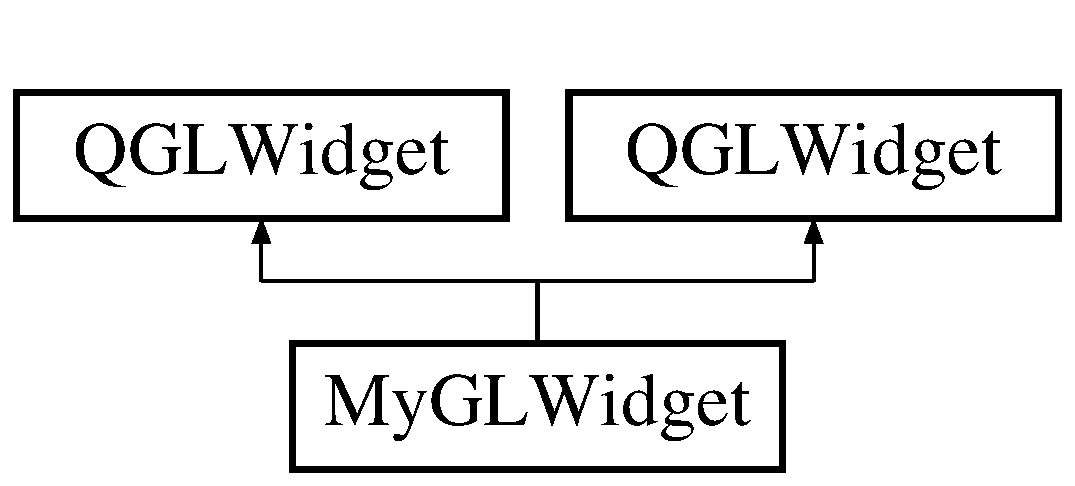
\includegraphics[height=2.000000cm]{classMyGLWidget}
\end{center}
\end{figure}
\subsection*{Typy publiczne}
\begin{DoxyCompactItemize}
\item 
enum \{ \hyperlink{classMyGLWidget_a349b4124c85266bef75a190246dca82eafafafccf4bbe772769c94573d5f3101e}{K\-O\-L\-O}, 
\hyperlink{classMyGLWidget_a349b4124c85266bef75a190246dca82ea83219b17f1da7d6ff531f1f616f1f497}{K\-W\-A\-D\-R\-A\-T}, 
\hyperlink{classMyGLWidget_a349b4124c85266bef75a190246dca82ead114f07fe7235d3994ecc8e8270ffbdf}{T\-R\-O\-J\-K\-A\-T}
 \}
\item 
enum \{ \hyperlink{classMyGLWidget_a349b4124c85266bef75a190246dca82eafafafccf4bbe772769c94573d5f3101e}{K\-O\-L\-O}, 
\hyperlink{classMyGLWidget_a349b4124c85266bef75a190246dca82ea83219b17f1da7d6ff531f1f616f1f497}{K\-W\-A\-D\-R\-A\-T}, 
\hyperlink{classMyGLWidget_a349b4124c85266bef75a190246dca82ead114f07fe7235d3994ecc8e8270ffbdf}{T\-R\-O\-J\-K\-A\-T}
 \}
\end{DoxyCompactItemize}
\subsection*{Sloty publiczne}
\begin{DoxyCompactItemize}
\item 
void \hyperlink{classMyGLWidget_ad0fe9c70e007c3ff7365083a9a4586ff}{on\-\_\-timer} ()
\item 
void \hyperlink{classMyGLWidget_ae42f967e5429aed3210ecffbe68ed537}{usun\-Figury\-Slot} ()
\end{DoxyCompactItemize}
\subsection*{Metody publiczne}
\begin{DoxyCompactItemize}
\item 
\hyperlink{classMyGLWidget_a2b3f2523eae378b2a4a5f66bd176be57}{My\-G\-L\-Widget} (Q\-Widget $\ast$parent=0)
\item 
virtual \hyperlink{classMyGLWidget_aefac459d382b61ea5589ff6269ecdf73}{$\sim$\-My\-G\-L\-Widget} ()
\item 
void \hyperlink{classMyGLWidget_af0ec25e9dee6351a690c26a392cde121}{przeslij\-Figury} (Q\-List$<$ \hyperlink{classFigura}{Figura} $\ast$ $>$ \&)
\item 
void \hyperlink{classMyGLWidget_a23624367d20ad8ca6a09f283ccb92c31}{przeslij\-Info} (Q\-List$<$ \hyperlink{classOdcinek}{Odcinek} $\ast$ $>$ \&, int \hyperlink{classMyGLWidget_ae1dab2275c515885d170d48a682d1943}{ramka\-Przyblizania}, int)
\item 
void \hyperlink{classMyGLWidget_a3cecbb2f5658f148e6e5d8ef3a3cc5e5}{zmien\-Ortho} (int)
\item 
\hyperlink{classMyGLWidget_a2b3f2523eae378b2a4a5f66bd176be57}{My\-G\-L\-Widget} (Q\-Widget $\ast$parent=0)
\item 
virtual \hyperlink{classMyGLWidget_a5ae6fab157bceedb032e074f519b9ad2}{$\sim$\-My\-G\-L\-Widget} ()
\item 
void \hyperlink{classMyGLWidget_a9859c9d91ca7457eadf69262c5b2766f}{dodaj\-Kwadrat} (float, float, float)
\item 
void \hyperlink{classMyGLWidget_a09ca4dbb3bb5714f5bf0dd531c7d5db9}{dodaj\-Kolo} (float, float, float)
\item 
void \hyperlink{classMyGLWidget_a35509c8dc1d449238eb960cc71c05204}{dodaj\-Trojkat} (float, float, float)
\end{DoxyCompactItemize}
\subsection*{Metody chronione}
\begin{DoxyCompactItemize}
\item 
void \hyperlink{classMyGLWidget_a5c536c2ebab76533eb16eac0a9830c8e}{initialize\-G\-L} ()
\item 
void \hyperlink{classMyGLWidget_adca50638295dc5d284f4f042331e82a0}{resize\-G\-L} (int w, int h)
\item 
void \hyperlink{classMyGLWidget_ad0e4171fab09ad54d4e2d23e7d6541eb}{paint\-G\-L} ()
\item 
void \hyperlink{classMyGLWidget_a98f0ba932652fe25ae3a469a9b6ee7e5}{mouse\-Press\-Event} (Q\-Mouse\-Event $\ast$)
\item 
void \hyperlink{classMyGLWidget_ac6f3e3d95c1d8b22325437d925812212}{mouse\-Move\-Event} (Q\-Mouse\-Event $\ast$)
\item 
void \hyperlink{classMyGLWidget_a55f9a6c836a9362f59976f86e98a34d8}{wheel\-Event} (Q\-Wheel\-Event $\ast$)
\item 
void \hyperlink{classMyGLWidget_a802184e7a48ae2a79f3daf4519e4fc66}{animacja\-Przyblizania} ()
\item 
void \hyperlink{classMyGLWidget_a5c536c2ebab76533eb16eac0a9830c8e}{initialize\-G\-L} ()
\item 
void \hyperlink{classMyGLWidget_adca50638295dc5d284f4f042331e82a0}{resize\-G\-L} (int w, int h)
\item 
void \hyperlink{classMyGLWidget_ad0e4171fab09ad54d4e2d23e7d6541eb}{paint\-G\-L} ()
\item 
void \hyperlink{classMyGLWidget_abb8eb0ad77ae3e49b96e85dafa1f1f30}{key\-Press\-Event} (Q\-Key\-Event $\ast$)
\item 
void \hyperlink{classMyGLWidget_a98f0ba932652fe25ae3a469a9b6ee7e5}{mouse\-Press\-Event} (Q\-Mouse\-Event $\ast$)
\item 
void \hyperlink{classMyGLWidget_ac6f3e3d95c1d8b22325437d925812212}{mouse\-Move\-Event} (Q\-Mouse\-Event $\ast$)
\item 
void \hyperlink{classMyGLWidget_a55f9a6c836a9362f59976f86e98a34d8}{wheel\-Event} (Q\-Wheel\-Event $\ast$)
\item 
void \hyperlink{classMyGLWidget_a817819b23bc4e0257e155d62f70578e0}{zmien\-Poziom} (int i)
\item 
void \hyperlink{classMyGLWidget_a802184e7a48ae2a79f3daf4519e4fc66}{animacja\-Przyblizania} ()
\item 
void \hyperlink{classMyGLWidget_ac089e8e36a522cc539d044d385ce83b3}{ruch\-Figur} ()
\item 
void \hyperlink{classMyGLWidget_ac4a465bd83a525cb73de97d29d30fe31}{zjadanie\-Mniejszych} ()
\item 
void \hyperlink{classMyGLWidget_a70e0c377b20ec2b13ea55071a1d7e7af}{ruch\-Odrzutowy} ()
\item 
void \hyperlink{classMyGLWidget_ae7df9920940250cc1f25dead0808b0a9}{usun\-Odicnki} ()
\end{DoxyCompactItemize}
\subsection*{Atrybuty chronione}
\begin{DoxyCompactItemize}
\item 
int \hyperlink{classMyGLWidget_a2a7fab72a9434ab8a32f67768f758011}{wartosc\-Ortho}
\item 
int \hyperlink{classMyGLWidget_ae1dab2275c515885d170d48a682d1943}{ramka\-Przyblizania}
\item 
G\-Lfloat \hyperlink{classMyGLWidget_a8d0f06e3361addec1ba11fe317de2c60}{tlo} \mbox{[}4\mbox{]}
\item 
Q\-List$<$ \hyperlink{classFigura}{Figura} $\ast$ $>$ \hyperlink{classMyGLWidget_abaf64d08c7bac0df986839ac063b02c2}{lista\-Figur}
\item 
Q\-List$<$ \hyperlink{classOdcinek}{Odcinek} $\ast$ $>$ \hyperlink{classMyGLWidget_a8bffb841dfb582085520d96a83ae09b9}{lista\-Odcinkow}
\item 
\hyperlink{classFigura}{Figura} $\ast$ \hyperlink{classMyGLWidget_afaf6be98dbfe311829f71f5b97ab6081}{sterowana}
\item 
Q\-Point\-F \hyperlink{classMyGLWidget_afc6be3de6cfab3079b8d36ab85d13317}{last\-Pos}
\item 
int \hyperlink{classMyGLWidget_ab3fcfaa0bcedb9ee1b56fdacf58499ba}{aktualny\-Poziom}
\item 
int \hyperlink{classMyGLWidget_aa3f67be6e4f2bf11f257d5843d17e8aa}{nr\-Klienta}
\item 
int \hyperlink{classMyGLWidget_abcd5810bea3e05c3c658491bd1d6fd43}{ramka}
\item 
\hyperlink{classPoziomy}{Poziomy} \hyperlink{classMyGLWidget_af24378be9ebc485231a336d72b9ae698}{poziomy}
\item 
Q\-Timer \hyperlink{classMyGLWidget_a5b154232ee1d21cc8b034e28798a5245}{timer}
\item 
int \hyperlink{classMyGLWidget_a0c89380896bd79421cd4c6fcae3e0e18}{Ts}
\end{DoxyCompactItemize}


\subsection{Dokumentacja składowych wyliczanych}
\hypertarget{classMyGLWidget_af113448149643de988f993f8aa85fd85}{\subsubsection[{anonymous enum}]{\setlength{\rightskip}{0pt plus 5cm}anonymous enum}}\label{classMyGLWidget_af113448149643de988f993f8aa85fd85}
\begin{Desc}
\item[Wartości wyliczeń]\par
\begin{description}
\index{K\-O\-L\-O@{K\-O\-L\-O}!My\-G\-L\-Widget@{My\-G\-L\-Widget}}\index{My\-G\-L\-Widget@{My\-G\-L\-Widget}!K\-O\-L\-O@{K\-O\-L\-O}}\item[{\em 
\hypertarget{classMyGLWidget_a349b4124c85266bef75a190246dca82eafafafccf4bbe772769c94573d5f3101e}{K\-O\-L\-O}\label{classMyGLWidget_a349b4124c85266bef75a190246dca82eafafafccf4bbe772769c94573d5f3101e}
}]\index{K\-W\-A\-D\-R\-A\-T@{K\-W\-A\-D\-R\-A\-T}!My\-G\-L\-Widget@{My\-G\-L\-Widget}}\index{My\-G\-L\-Widget@{My\-G\-L\-Widget}!K\-W\-A\-D\-R\-A\-T@{K\-W\-A\-D\-R\-A\-T}}\item[{\em 
\hypertarget{classMyGLWidget_a349b4124c85266bef75a190246dca82ea83219b17f1da7d6ff531f1f616f1f497}{K\-W\-A\-D\-R\-A\-T}\label{classMyGLWidget_a349b4124c85266bef75a190246dca82ea83219b17f1da7d6ff531f1f616f1f497}
}]\index{T\-R\-O\-J\-K\-A\-T@{T\-R\-O\-J\-K\-A\-T}!My\-G\-L\-Widget@{My\-G\-L\-Widget}}\index{My\-G\-L\-Widget@{My\-G\-L\-Widget}!T\-R\-O\-J\-K\-A\-T@{T\-R\-O\-J\-K\-A\-T}}\item[{\em 
\hypertarget{classMyGLWidget_a349b4124c85266bef75a190246dca82ead114f07fe7235d3994ecc8e8270ffbdf}{T\-R\-O\-J\-K\-A\-T}\label{classMyGLWidget_a349b4124c85266bef75a190246dca82ead114f07fe7235d3994ecc8e8270ffbdf}
}]\end{description}
\end{Desc}
\hypertarget{classMyGLWidget_a349b4124c85266bef75a190246dca82e}{\subsubsection[{anonymous enum}]{\setlength{\rightskip}{0pt plus 5cm}anonymous enum}}\label{classMyGLWidget_a349b4124c85266bef75a190246dca82e}
\begin{Desc}
\item[Wartości wyliczeń]\par
\begin{description}
\index{K\-O\-L\-O@{K\-O\-L\-O}!My\-G\-L\-Widget@{My\-G\-L\-Widget}}\index{My\-G\-L\-Widget@{My\-G\-L\-Widget}!K\-O\-L\-O@{K\-O\-L\-O}}\item[{\em 
\hypertarget{classMyGLWidget_a349b4124c85266bef75a190246dca82eafafafccf4bbe772769c94573d5f3101e}{K\-O\-L\-O}\label{classMyGLWidget_a349b4124c85266bef75a190246dca82eafafafccf4bbe772769c94573d5f3101e}
}]\index{K\-W\-A\-D\-R\-A\-T@{K\-W\-A\-D\-R\-A\-T}!My\-G\-L\-Widget@{My\-G\-L\-Widget}}\index{My\-G\-L\-Widget@{My\-G\-L\-Widget}!K\-W\-A\-D\-R\-A\-T@{K\-W\-A\-D\-R\-A\-T}}\item[{\em 
\hypertarget{classMyGLWidget_a349b4124c85266bef75a190246dca82ea83219b17f1da7d6ff531f1f616f1f497}{K\-W\-A\-D\-R\-A\-T}\label{classMyGLWidget_a349b4124c85266bef75a190246dca82ea83219b17f1da7d6ff531f1f616f1f497}
}]\index{T\-R\-O\-J\-K\-A\-T@{T\-R\-O\-J\-K\-A\-T}!My\-G\-L\-Widget@{My\-G\-L\-Widget}}\index{My\-G\-L\-Widget@{My\-G\-L\-Widget}!T\-R\-O\-J\-K\-A\-T@{T\-R\-O\-J\-K\-A\-T}}\item[{\em 
\hypertarget{classMyGLWidget_a349b4124c85266bef75a190246dca82ead114f07fe7235d3994ecc8e8270ffbdf}{T\-R\-O\-J\-K\-A\-T}\label{classMyGLWidget_a349b4124c85266bef75a190246dca82ead114f07fe7235d3994ecc8e8270ffbdf}
}]\end{description}
\end{Desc}


\subsection{Dokumentacja konstruktora i destruktora}
\hypertarget{classMyGLWidget_a2b3f2523eae378b2a4a5f66bd176be57}{\index{My\-G\-L\-Widget@{My\-G\-L\-Widget}!My\-G\-L\-Widget@{My\-G\-L\-Widget}}
\index{My\-G\-L\-Widget@{My\-G\-L\-Widget}!MyGLWidget@{My\-G\-L\-Widget}}
\subsubsection[{My\-G\-L\-Widget}]{\setlength{\rightskip}{0pt plus 5cm}My\-G\-L\-Widget\-::\-My\-G\-L\-Widget (
\begin{DoxyParamCaption}
\item[{Q\-Widget $\ast$}]{parent = {\ttfamily 0}}
\end{DoxyParamCaption}
)\hspace{0.3cm}{\ttfamily [explicit]}}}\label{classMyGLWidget_a2b3f2523eae378b2a4a5f66bd176be57}
\hypertarget{classMyGLWidget_aefac459d382b61ea5589ff6269ecdf73}{\index{My\-G\-L\-Widget@{My\-G\-L\-Widget}!$\sim$\-My\-G\-L\-Widget@{$\sim$\-My\-G\-L\-Widget}}
\index{$\sim$\-My\-G\-L\-Widget@{$\sim$\-My\-G\-L\-Widget}!MyGLWidget@{My\-G\-L\-Widget}}
\subsubsection[{$\sim$\-My\-G\-L\-Widget}]{\setlength{\rightskip}{0pt plus 5cm}My\-G\-L\-Widget\-::$\sim$\-My\-G\-L\-Widget (
\begin{DoxyParamCaption}
{}
\end{DoxyParamCaption}
)\hspace{0.3cm}{\ttfamily [virtual]}}}\label{classMyGLWidget_aefac459d382b61ea5589ff6269ecdf73}
\hypertarget{classMyGLWidget_a2b3f2523eae378b2a4a5f66bd176be57}{\index{My\-G\-L\-Widget@{My\-G\-L\-Widget}!My\-G\-L\-Widget@{My\-G\-L\-Widget}}
\index{My\-G\-L\-Widget@{My\-G\-L\-Widget}!MyGLWidget@{My\-G\-L\-Widget}}
\subsubsection[{My\-G\-L\-Widget}]{\setlength{\rightskip}{0pt plus 5cm}My\-G\-L\-Widget\-::\-My\-G\-L\-Widget (
\begin{DoxyParamCaption}
\item[{Q\-Widget $\ast$}]{parent = {\ttfamily 0}}
\end{DoxyParamCaption}
)\hspace{0.3cm}{\ttfamily [explicit]}}}\label{classMyGLWidget_a2b3f2523eae378b2a4a5f66bd176be57}
\hypertarget{classMyGLWidget_a5ae6fab157bceedb032e074f519b9ad2}{\index{My\-G\-L\-Widget@{My\-G\-L\-Widget}!$\sim$\-My\-G\-L\-Widget@{$\sim$\-My\-G\-L\-Widget}}
\index{$\sim$\-My\-G\-L\-Widget@{$\sim$\-My\-G\-L\-Widget}!MyGLWidget@{My\-G\-L\-Widget}}
\subsubsection[{$\sim$\-My\-G\-L\-Widget}]{\setlength{\rightskip}{0pt plus 5cm}virtual My\-G\-L\-Widget\-::$\sim$\-My\-G\-L\-Widget (
\begin{DoxyParamCaption}
{}
\end{DoxyParamCaption}
)\hspace{0.3cm}{\ttfamily [virtual]}}}\label{classMyGLWidget_a5ae6fab157bceedb032e074f519b9ad2}


\subsection{Dokumentacja funkcji składowych}
\hypertarget{classMyGLWidget_a802184e7a48ae2a79f3daf4519e4fc66}{\index{My\-G\-L\-Widget@{My\-G\-L\-Widget}!animacja\-Przyblizania@{animacja\-Przyblizania}}
\index{animacja\-Przyblizania@{animacja\-Przyblizania}!MyGLWidget@{My\-G\-L\-Widget}}
\subsubsection[{animacja\-Przyblizania}]{\setlength{\rightskip}{0pt plus 5cm}void My\-G\-L\-Widget\-::animacja\-Przyblizania (
\begin{DoxyParamCaption}
{}
\end{DoxyParamCaption}
)\hspace{0.3cm}{\ttfamily [protected]}}}\label{classMyGLWidget_a802184e7a48ae2a79f3daf4519e4fc66}
\hypertarget{classMyGLWidget_a802184e7a48ae2a79f3daf4519e4fc66}{\index{My\-G\-L\-Widget@{My\-G\-L\-Widget}!animacja\-Przyblizania@{animacja\-Przyblizania}}
\index{animacja\-Przyblizania@{animacja\-Przyblizania}!MyGLWidget@{My\-G\-L\-Widget}}
\subsubsection[{animacja\-Przyblizania}]{\setlength{\rightskip}{0pt plus 5cm}void My\-G\-L\-Widget\-::animacja\-Przyblizania (
\begin{DoxyParamCaption}
{}
\end{DoxyParamCaption}
)\hspace{0.3cm}{\ttfamily [protected]}}}\label{classMyGLWidget_a802184e7a48ae2a79f3daf4519e4fc66}
\hypertarget{classMyGLWidget_a09ca4dbb3bb5714f5bf0dd531c7d5db9}{\index{My\-G\-L\-Widget@{My\-G\-L\-Widget}!dodaj\-Kolo@{dodaj\-Kolo}}
\index{dodaj\-Kolo@{dodaj\-Kolo}!MyGLWidget@{My\-G\-L\-Widget}}
\subsubsection[{dodaj\-Kolo}]{\setlength{\rightskip}{0pt plus 5cm}void My\-G\-L\-Widget\-::dodaj\-Kolo (
\begin{DoxyParamCaption}
\item[{float}]{x, }
\item[{float}]{y, }
\item[{float}]{r}
\end{DoxyParamCaption}
)}}\label{classMyGLWidget_a09ca4dbb3bb5714f5bf0dd531c7d5db9}
\hypertarget{classMyGLWidget_a9859c9d91ca7457eadf69262c5b2766f}{\index{My\-G\-L\-Widget@{My\-G\-L\-Widget}!dodaj\-Kwadrat@{dodaj\-Kwadrat}}
\index{dodaj\-Kwadrat@{dodaj\-Kwadrat}!MyGLWidget@{My\-G\-L\-Widget}}
\subsubsection[{dodaj\-Kwadrat}]{\setlength{\rightskip}{0pt plus 5cm}void My\-G\-L\-Widget\-::dodaj\-Kwadrat (
\begin{DoxyParamCaption}
\item[{float}]{x, }
\item[{float}]{y, }
\item[{float}]{a}
\end{DoxyParamCaption}
)}}\label{classMyGLWidget_a9859c9d91ca7457eadf69262c5b2766f}
\hypertarget{classMyGLWidget_a35509c8dc1d449238eb960cc71c05204}{\index{My\-G\-L\-Widget@{My\-G\-L\-Widget}!dodaj\-Trojkat@{dodaj\-Trojkat}}
\index{dodaj\-Trojkat@{dodaj\-Trojkat}!MyGLWidget@{My\-G\-L\-Widget}}
\subsubsection[{dodaj\-Trojkat}]{\setlength{\rightskip}{0pt plus 5cm}void My\-G\-L\-Widget\-::dodaj\-Trojkat (
\begin{DoxyParamCaption}
\item[{float}]{x, }
\item[{float}]{y, }
\item[{float}]{a}
\end{DoxyParamCaption}
)}}\label{classMyGLWidget_a35509c8dc1d449238eb960cc71c05204}
\hypertarget{classMyGLWidget_a5c536c2ebab76533eb16eac0a9830c8e}{\index{My\-G\-L\-Widget@{My\-G\-L\-Widget}!initialize\-G\-L@{initialize\-G\-L}}
\index{initialize\-G\-L@{initialize\-G\-L}!MyGLWidget@{My\-G\-L\-Widget}}
\subsubsection[{initialize\-G\-L}]{\setlength{\rightskip}{0pt plus 5cm}void My\-G\-L\-Widget\-::initialize\-G\-L (
\begin{DoxyParamCaption}
{}
\end{DoxyParamCaption}
)\hspace{0.3cm}{\ttfamily [protected]}}}\label{classMyGLWidget_a5c536c2ebab76533eb16eac0a9830c8e}
\hypertarget{classMyGLWidget_a5c536c2ebab76533eb16eac0a9830c8e}{\index{My\-G\-L\-Widget@{My\-G\-L\-Widget}!initialize\-G\-L@{initialize\-G\-L}}
\index{initialize\-G\-L@{initialize\-G\-L}!MyGLWidget@{My\-G\-L\-Widget}}
\subsubsection[{initialize\-G\-L}]{\setlength{\rightskip}{0pt plus 5cm}void My\-G\-L\-Widget\-::initialize\-G\-L (
\begin{DoxyParamCaption}
{}
\end{DoxyParamCaption}
)\hspace{0.3cm}{\ttfamily [protected]}}}\label{classMyGLWidget_a5c536c2ebab76533eb16eac0a9830c8e}
\hypertarget{classMyGLWidget_abb8eb0ad77ae3e49b96e85dafa1f1f30}{\index{My\-G\-L\-Widget@{My\-G\-L\-Widget}!key\-Press\-Event@{key\-Press\-Event}}
\index{key\-Press\-Event@{key\-Press\-Event}!MyGLWidget@{My\-G\-L\-Widget}}
\subsubsection[{key\-Press\-Event}]{\setlength{\rightskip}{0pt plus 5cm}void My\-G\-L\-Widget\-::key\-Press\-Event (
\begin{DoxyParamCaption}
\item[{Q\-Key\-Event $\ast$}]{event}
\end{DoxyParamCaption}
)\hspace{0.3cm}{\ttfamily [protected]}}}\label{classMyGLWidget_abb8eb0ad77ae3e49b96e85dafa1f1f30}
\hypertarget{classMyGLWidget_ac6f3e3d95c1d8b22325437d925812212}{\index{My\-G\-L\-Widget@{My\-G\-L\-Widget}!mouse\-Move\-Event@{mouse\-Move\-Event}}
\index{mouse\-Move\-Event@{mouse\-Move\-Event}!MyGLWidget@{My\-G\-L\-Widget}}
\subsubsection[{mouse\-Move\-Event}]{\setlength{\rightskip}{0pt plus 5cm}void My\-G\-L\-Widget\-::mouse\-Move\-Event (
\begin{DoxyParamCaption}
\item[{Q\-Mouse\-Event $\ast$}]{}
\end{DoxyParamCaption}
)\hspace{0.3cm}{\ttfamily [protected]}}}\label{classMyGLWidget_ac6f3e3d95c1d8b22325437d925812212}
\hypertarget{classMyGLWidget_ac6f3e3d95c1d8b22325437d925812212}{\index{My\-G\-L\-Widget@{My\-G\-L\-Widget}!mouse\-Move\-Event@{mouse\-Move\-Event}}
\index{mouse\-Move\-Event@{mouse\-Move\-Event}!MyGLWidget@{My\-G\-L\-Widget}}
\subsubsection[{mouse\-Move\-Event}]{\setlength{\rightskip}{0pt plus 5cm}void My\-G\-L\-Widget\-::mouse\-Move\-Event (
\begin{DoxyParamCaption}
\item[{Q\-Mouse\-Event $\ast$}]{event}
\end{DoxyParamCaption}
)\hspace{0.3cm}{\ttfamily [protected]}}}\label{classMyGLWidget_ac6f3e3d95c1d8b22325437d925812212}
\hypertarget{classMyGLWidget_a98f0ba932652fe25ae3a469a9b6ee7e5}{\index{My\-G\-L\-Widget@{My\-G\-L\-Widget}!mouse\-Press\-Event@{mouse\-Press\-Event}}
\index{mouse\-Press\-Event@{mouse\-Press\-Event}!MyGLWidget@{My\-G\-L\-Widget}}
\subsubsection[{mouse\-Press\-Event}]{\setlength{\rightskip}{0pt plus 5cm}void My\-G\-L\-Widget\-::mouse\-Press\-Event (
\begin{DoxyParamCaption}
\item[{Q\-Mouse\-Event $\ast$}]{}
\end{DoxyParamCaption}
)\hspace{0.3cm}{\ttfamily [protected]}}}\label{classMyGLWidget_a98f0ba932652fe25ae3a469a9b6ee7e5}
\hypertarget{classMyGLWidget_a98f0ba932652fe25ae3a469a9b6ee7e5}{\index{My\-G\-L\-Widget@{My\-G\-L\-Widget}!mouse\-Press\-Event@{mouse\-Press\-Event}}
\index{mouse\-Press\-Event@{mouse\-Press\-Event}!MyGLWidget@{My\-G\-L\-Widget}}
\subsubsection[{mouse\-Press\-Event}]{\setlength{\rightskip}{0pt plus 5cm}void My\-G\-L\-Widget\-::mouse\-Press\-Event (
\begin{DoxyParamCaption}
\item[{Q\-Mouse\-Event $\ast$}]{event}
\end{DoxyParamCaption}
)\hspace{0.3cm}{\ttfamily [protected]}}}\label{classMyGLWidget_a98f0ba932652fe25ae3a469a9b6ee7e5}
\hypertarget{classMyGLWidget_ad0fe9c70e007c3ff7365083a9a4586ff}{\index{My\-G\-L\-Widget@{My\-G\-L\-Widget}!on\-\_\-timer@{on\-\_\-timer}}
\index{on\-\_\-timer@{on\-\_\-timer}!MyGLWidget@{My\-G\-L\-Widget}}
\subsubsection[{on\-\_\-timer}]{\setlength{\rightskip}{0pt plus 5cm}void My\-G\-L\-Widget\-::on\-\_\-timer (
\begin{DoxyParamCaption}
{}
\end{DoxyParamCaption}
)\hspace{0.3cm}{\ttfamily [slot]}}}\label{classMyGLWidget_ad0fe9c70e007c3ff7365083a9a4586ff}
\hypertarget{classMyGLWidget_ad0e4171fab09ad54d4e2d23e7d6541eb}{\index{My\-G\-L\-Widget@{My\-G\-L\-Widget}!paint\-G\-L@{paint\-G\-L}}
\index{paint\-G\-L@{paint\-G\-L}!MyGLWidget@{My\-G\-L\-Widget}}
\subsubsection[{paint\-G\-L}]{\setlength{\rightskip}{0pt plus 5cm}void My\-G\-L\-Widget\-::paint\-G\-L (
\begin{DoxyParamCaption}
{}
\end{DoxyParamCaption}
)\hspace{0.3cm}{\ttfamily [protected]}}}\label{classMyGLWidget_ad0e4171fab09ad54d4e2d23e7d6541eb}
\hypertarget{classMyGLWidget_ad0e4171fab09ad54d4e2d23e7d6541eb}{\index{My\-G\-L\-Widget@{My\-G\-L\-Widget}!paint\-G\-L@{paint\-G\-L}}
\index{paint\-G\-L@{paint\-G\-L}!MyGLWidget@{My\-G\-L\-Widget}}
\subsubsection[{paint\-G\-L}]{\setlength{\rightskip}{0pt plus 5cm}void My\-G\-L\-Widget\-::paint\-G\-L (
\begin{DoxyParamCaption}
{}
\end{DoxyParamCaption}
)\hspace{0.3cm}{\ttfamily [protected]}}}\label{classMyGLWidget_ad0e4171fab09ad54d4e2d23e7d6541eb}
\hypertarget{classMyGLWidget_af0ec25e9dee6351a690c26a392cde121}{\index{My\-G\-L\-Widget@{My\-G\-L\-Widget}!przeslij\-Figury@{przeslij\-Figury}}
\index{przeslij\-Figury@{przeslij\-Figury}!MyGLWidget@{My\-G\-L\-Widget}}
\subsubsection[{przeslij\-Figury}]{\setlength{\rightskip}{0pt plus 5cm}void My\-G\-L\-Widget\-::przeslij\-Figury (
\begin{DoxyParamCaption}
\item[{Q\-List$<$ {\bf Figura} $\ast$ $>$ \&}]{list1}
\end{DoxyParamCaption}
)}}\label{classMyGLWidget_af0ec25e9dee6351a690c26a392cde121}
\hypertarget{classMyGLWidget_a23624367d20ad8ca6a09f283ccb92c31}{\index{My\-G\-L\-Widget@{My\-G\-L\-Widget}!przeslij\-Info@{przeslij\-Info}}
\index{przeslij\-Info@{przeslij\-Info}!MyGLWidget@{My\-G\-L\-Widget}}
\subsubsection[{przeslij\-Info}]{\setlength{\rightskip}{0pt plus 5cm}void My\-G\-L\-Widget\-::przeslij\-Info (
\begin{DoxyParamCaption}
\item[{Q\-List$<$ {\bf Odcinek} $\ast$ $>$ \&}]{list1, }
\item[{int}]{ramka\-Przyblizania, }
\item[{int}]{nr\-Klienta\-\_\-}
\end{DoxyParamCaption}
)}}\label{classMyGLWidget_a23624367d20ad8ca6a09f283ccb92c31}
\hypertarget{classMyGLWidget_adca50638295dc5d284f4f042331e82a0}{\index{My\-G\-L\-Widget@{My\-G\-L\-Widget}!resize\-G\-L@{resize\-G\-L}}
\index{resize\-G\-L@{resize\-G\-L}!MyGLWidget@{My\-G\-L\-Widget}}
\subsubsection[{resize\-G\-L}]{\setlength{\rightskip}{0pt plus 5cm}void My\-G\-L\-Widget\-::resize\-G\-L (
\begin{DoxyParamCaption}
\item[{int}]{w, }
\item[{int}]{h}
\end{DoxyParamCaption}
)\hspace{0.3cm}{\ttfamily [protected]}}}\label{classMyGLWidget_adca50638295dc5d284f4f042331e82a0}
\hypertarget{classMyGLWidget_adca50638295dc5d284f4f042331e82a0}{\index{My\-G\-L\-Widget@{My\-G\-L\-Widget}!resize\-G\-L@{resize\-G\-L}}
\index{resize\-G\-L@{resize\-G\-L}!MyGLWidget@{My\-G\-L\-Widget}}
\subsubsection[{resize\-G\-L}]{\setlength{\rightskip}{0pt plus 5cm}void My\-G\-L\-Widget\-::resize\-G\-L (
\begin{DoxyParamCaption}
\item[{int}]{w, }
\item[{int}]{h}
\end{DoxyParamCaption}
)\hspace{0.3cm}{\ttfamily [protected]}}}\label{classMyGLWidget_adca50638295dc5d284f4f042331e82a0}
\hypertarget{classMyGLWidget_ac089e8e36a522cc539d044d385ce83b3}{\index{My\-G\-L\-Widget@{My\-G\-L\-Widget}!ruch\-Figur@{ruch\-Figur}}
\index{ruch\-Figur@{ruch\-Figur}!MyGLWidget@{My\-G\-L\-Widget}}
\subsubsection[{ruch\-Figur}]{\setlength{\rightskip}{0pt plus 5cm}void My\-G\-L\-Widget\-::ruch\-Figur (
\begin{DoxyParamCaption}
{}
\end{DoxyParamCaption}
)\hspace{0.3cm}{\ttfamily [protected]}}}\label{classMyGLWidget_ac089e8e36a522cc539d044d385ce83b3}
\hypertarget{classMyGLWidget_a70e0c377b20ec2b13ea55071a1d7e7af}{\index{My\-G\-L\-Widget@{My\-G\-L\-Widget}!ruch\-Odrzutowy@{ruch\-Odrzutowy}}
\index{ruch\-Odrzutowy@{ruch\-Odrzutowy}!MyGLWidget@{My\-G\-L\-Widget}}
\subsubsection[{ruch\-Odrzutowy}]{\setlength{\rightskip}{0pt plus 5cm}void My\-G\-L\-Widget\-::ruch\-Odrzutowy (
\begin{DoxyParamCaption}
{}
\end{DoxyParamCaption}
)\hspace{0.3cm}{\ttfamily [protected]}}}\label{classMyGLWidget_a70e0c377b20ec2b13ea55071a1d7e7af}
\hypertarget{classMyGLWidget_ae42f967e5429aed3210ecffbe68ed537}{\index{My\-G\-L\-Widget@{My\-G\-L\-Widget}!usun\-Figury\-Slot@{usun\-Figury\-Slot}}
\index{usun\-Figury\-Slot@{usun\-Figury\-Slot}!MyGLWidget@{My\-G\-L\-Widget}}
\subsubsection[{usun\-Figury\-Slot}]{\setlength{\rightskip}{0pt plus 5cm}void My\-G\-L\-Widget\-::usun\-Figury\-Slot (
\begin{DoxyParamCaption}
{}
\end{DoxyParamCaption}
)\hspace{0.3cm}{\ttfamily [slot]}}}\label{classMyGLWidget_ae42f967e5429aed3210ecffbe68ed537}
\hypertarget{classMyGLWidget_ae7df9920940250cc1f25dead0808b0a9}{\index{My\-G\-L\-Widget@{My\-G\-L\-Widget}!usun\-Odicnki@{usun\-Odicnki}}
\index{usun\-Odicnki@{usun\-Odicnki}!MyGLWidget@{My\-G\-L\-Widget}}
\subsubsection[{usun\-Odicnki}]{\setlength{\rightskip}{0pt plus 5cm}void My\-G\-L\-Widget\-::usun\-Odicnki (
\begin{DoxyParamCaption}
{}
\end{DoxyParamCaption}
)\hspace{0.3cm}{\ttfamily [protected]}}}\label{classMyGLWidget_ae7df9920940250cc1f25dead0808b0a9}
\hypertarget{classMyGLWidget_a55f9a6c836a9362f59976f86e98a34d8}{\index{My\-G\-L\-Widget@{My\-G\-L\-Widget}!wheel\-Event@{wheel\-Event}}
\index{wheel\-Event@{wheel\-Event}!MyGLWidget@{My\-G\-L\-Widget}}
\subsubsection[{wheel\-Event}]{\setlength{\rightskip}{0pt plus 5cm}void My\-G\-L\-Widget\-::wheel\-Event (
\begin{DoxyParamCaption}
\item[{Q\-Wheel\-Event $\ast$}]{}
\end{DoxyParamCaption}
)\hspace{0.3cm}{\ttfamily [protected]}}}\label{classMyGLWidget_a55f9a6c836a9362f59976f86e98a34d8}
\hypertarget{classMyGLWidget_a55f9a6c836a9362f59976f86e98a34d8}{\index{My\-G\-L\-Widget@{My\-G\-L\-Widget}!wheel\-Event@{wheel\-Event}}
\index{wheel\-Event@{wheel\-Event}!MyGLWidget@{My\-G\-L\-Widget}}
\subsubsection[{wheel\-Event}]{\setlength{\rightskip}{0pt plus 5cm}void My\-G\-L\-Widget\-::wheel\-Event (
\begin{DoxyParamCaption}
\item[{Q\-Wheel\-Event $\ast$}]{event}
\end{DoxyParamCaption}
)\hspace{0.3cm}{\ttfamily [protected]}}}\label{classMyGLWidget_a55f9a6c836a9362f59976f86e98a34d8}
\hypertarget{classMyGLWidget_ac4a465bd83a525cb73de97d29d30fe31}{\index{My\-G\-L\-Widget@{My\-G\-L\-Widget}!zjadanie\-Mniejszych@{zjadanie\-Mniejszych}}
\index{zjadanie\-Mniejszych@{zjadanie\-Mniejszych}!MyGLWidget@{My\-G\-L\-Widget}}
\subsubsection[{zjadanie\-Mniejszych}]{\setlength{\rightskip}{0pt plus 5cm}void My\-G\-L\-Widget\-::zjadanie\-Mniejszych (
\begin{DoxyParamCaption}
{}
\end{DoxyParamCaption}
)\hspace{0.3cm}{\ttfamily [protected]}}}\label{classMyGLWidget_ac4a465bd83a525cb73de97d29d30fe31}
\hypertarget{classMyGLWidget_a3cecbb2f5658f148e6e5d8ef3a3cc5e5}{\index{My\-G\-L\-Widget@{My\-G\-L\-Widget}!zmien\-Ortho@{zmien\-Ortho}}
\index{zmien\-Ortho@{zmien\-Ortho}!MyGLWidget@{My\-G\-L\-Widget}}
\subsubsection[{zmien\-Ortho}]{\setlength{\rightskip}{0pt plus 5cm}void My\-G\-L\-Widget\-::zmien\-Ortho (
\begin{DoxyParamCaption}
\item[{int}]{value}
\end{DoxyParamCaption}
)}}\label{classMyGLWidget_a3cecbb2f5658f148e6e5d8ef3a3cc5e5}
\hypertarget{classMyGLWidget_a817819b23bc4e0257e155d62f70578e0}{\index{My\-G\-L\-Widget@{My\-G\-L\-Widget}!zmien\-Poziom@{zmien\-Poziom}}
\index{zmien\-Poziom@{zmien\-Poziom}!MyGLWidget@{My\-G\-L\-Widget}}
\subsubsection[{zmien\-Poziom}]{\setlength{\rightskip}{0pt plus 5cm}void My\-G\-L\-Widget\-::zmien\-Poziom (
\begin{DoxyParamCaption}
\item[{int}]{i}
\end{DoxyParamCaption}
)\hspace{0.3cm}{\ttfamily [protected]}}}\label{classMyGLWidget_a817819b23bc4e0257e155d62f70578e0}


\subsection{Dokumentacja atrybutów składowych}
\hypertarget{classMyGLWidget_ab3fcfaa0bcedb9ee1b56fdacf58499ba}{\index{My\-G\-L\-Widget@{My\-G\-L\-Widget}!aktualny\-Poziom@{aktualny\-Poziom}}
\index{aktualny\-Poziom@{aktualny\-Poziom}!MyGLWidget@{My\-G\-L\-Widget}}
\subsubsection[{aktualny\-Poziom}]{\setlength{\rightskip}{0pt plus 5cm}int My\-G\-L\-Widget\-::aktualny\-Poziom\hspace{0.3cm}{\ttfamily [protected]}}}\label{classMyGLWidget_ab3fcfaa0bcedb9ee1b56fdacf58499ba}
\hypertarget{classMyGLWidget_afc6be3de6cfab3079b8d36ab85d13317}{\index{My\-G\-L\-Widget@{My\-G\-L\-Widget}!last\-Pos@{last\-Pos}}
\index{last\-Pos@{last\-Pos}!MyGLWidget@{My\-G\-L\-Widget}}
\subsubsection[{last\-Pos}]{\setlength{\rightskip}{0pt plus 5cm}Q\-Point\-F My\-G\-L\-Widget\-::last\-Pos\hspace{0.3cm}{\ttfamily [protected]}}}\label{classMyGLWidget_afc6be3de6cfab3079b8d36ab85d13317}
\hypertarget{classMyGLWidget_abaf64d08c7bac0df986839ac063b02c2}{\index{My\-G\-L\-Widget@{My\-G\-L\-Widget}!lista\-Figur@{lista\-Figur}}
\index{lista\-Figur@{lista\-Figur}!MyGLWidget@{My\-G\-L\-Widget}}
\subsubsection[{lista\-Figur}]{\setlength{\rightskip}{0pt plus 5cm}Q\-List$<$ {\bf Figura} $\ast$ $>$ My\-G\-L\-Widget\-::lista\-Figur\hspace{0.3cm}{\ttfamily [protected]}}}\label{classMyGLWidget_abaf64d08c7bac0df986839ac063b02c2}
\hypertarget{classMyGLWidget_a8bffb841dfb582085520d96a83ae09b9}{\index{My\-G\-L\-Widget@{My\-G\-L\-Widget}!lista\-Odcinkow@{lista\-Odcinkow}}
\index{lista\-Odcinkow@{lista\-Odcinkow}!MyGLWidget@{My\-G\-L\-Widget}}
\subsubsection[{lista\-Odcinkow}]{\setlength{\rightskip}{0pt plus 5cm}Q\-List$<$ {\bf Odcinek} $\ast$ $>$ My\-G\-L\-Widget\-::lista\-Odcinkow\hspace{0.3cm}{\ttfamily [protected]}}}\label{classMyGLWidget_a8bffb841dfb582085520d96a83ae09b9}
\hypertarget{classMyGLWidget_aa3f67be6e4f2bf11f257d5843d17e8aa}{\index{My\-G\-L\-Widget@{My\-G\-L\-Widget}!nr\-Klienta@{nr\-Klienta}}
\index{nr\-Klienta@{nr\-Klienta}!MyGLWidget@{My\-G\-L\-Widget}}
\subsubsection[{nr\-Klienta}]{\setlength{\rightskip}{0pt plus 5cm}int My\-G\-L\-Widget\-::nr\-Klienta\hspace{0.3cm}{\ttfamily [protected]}}}\label{classMyGLWidget_aa3f67be6e4f2bf11f257d5843d17e8aa}
\hypertarget{classMyGLWidget_af24378be9ebc485231a336d72b9ae698}{\index{My\-G\-L\-Widget@{My\-G\-L\-Widget}!poziomy@{poziomy}}
\index{poziomy@{poziomy}!MyGLWidget@{My\-G\-L\-Widget}}
\subsubsection[{poziomy}]{\setlength{\rightskip}{0pt plus 5cm}{\bf Poziomy} My\-G\-L\-Widget\-::poziomy\hspace{0.3cm}{\ttfamily [protected]}}}\label{classMyGLWidget_af24378be9ebc485231a336d72b9ae698}
\hypertarget{classMyGLWidget_abcd5810bea3e05c3c658491bd1d6fd43}{\index{My\-G\-L\-Widget@{My\-G\-L\-Widget}!ramka@{ramka}}
\index{ramka@{ramka}!MyGLWidget@{My\-G\-L\-Widget}}
\subsubsection[{ramka}]{\setlength{\rightskip}{0pt plus 5cm}int My\-G\-L\-Widget\-::ramka\hspace{0.3cm}{\ttfamily [protected]}}}\label{classMyGLWidget_abcd5810bea3e05c3c658491bd1d6fd43}
\hypertarget{classMyGLWidget_ae1dab2275c515885d170d48a682d1943}{\index{My\-G\-L\-Widget@{My\-G\-L\-Widget}!ramka\-Przyblizania@{ramka\-Przyblizania}}
\index{ramka\-Przyblizania@{ramka\-Przyblizania}!MyGLWidget@{My\-G\-L\-Widget}}
\subsubsection[{ramka\-Przyblizania}]{\setlength{\rightskip}{0pt plus 5cm}int My\-G\-L\-Widget\-::ramka\-Przyblizania\hspace{0.3cm}{\ttfamily [protected]}}}\label{classMyGLWidget_ae1dab2275c515885d170d48a682d1943}
\hypertarget{classMyGLWidget_afaf6be98dbfe311829f71f5b97ab6081}{\index{My\-G\-L\-Widget@{My\-G\-L\-Widget}!sterowana@{sterowana}}
\index{sterowana@{sterowana}!MyGLWidget@{My\-G\-L\-Widget}}
\subsubsection[{sterowana}]{\setlength{\rightskip}{0pt plus 5cm}{\bf Figura} $\ast$ My\-G\-L\-Widget\-::sterowana\hspace{0.3cm}{\ttfamily [protected]}}}\label{classMyGLWidget_afaf6be98dbfe311829f71f5b97ab6081}
\hypertarget{classMyGLWidget_a5b154232ee1d21cc8b034e28798a5245}{\index{My\-G\-L\-Widget@{My\-G\-L\-Widget}!timer@{timer}}
\index{timer@{timer}!MyGLWidget@{My\-G\-L\-Widget}}
\subsubsection[{timer}]{\setlength{\rightskip}{0pt plus 5cm}Q\-Timer My\-G\-L\-Widget\-::timer\hspace{0.3cm}{\ttfamily [protected]}}}\label{classMyGLWidget_a5b154232ee1d21cc8b034e28798a5245}
\hypertarget{classMyGLWidget_a8d0f06e3361addec1ba11fe317de2c60}{\index{My\-G\-L\-Widget@{My\-G\-L\-Widget}!tlo@{tlo}}
\index{tlo@{tlo}!MyGLWidget@{My\-G\-L\-Widget}}
\subsubsection[{tlo}]{\setlength{\rightskip}{0pt plus 5cm}G\-Lfloat My\-G\-L\-Widget\-::tlo\hspace{0.3cm}{\ttfamily [protected]}}}\label{classMyGLWidget_a8d0f06e3361addec1ba11fe317de2c60}
\hypertarget{classMyGLWidget_a0c89380896bd79421cd4c6fcae3e0e18}{\index{My\-G\-L\-Widget@{My\-G\-L\-Widget}!Ts@{Ts}}
\index{Ts@{Ts}!MyGLWidget@{My\-G\-L\-Widget}}
\subsubsection[{Ts}]{\setlength{\rightskip}{0pt plus 5cm}int My\-G\-L\-Widget\-::\-Ts\hspace{0.3cm}{\ttfamily [protected]}}}\label{classMyGLWidget_a0c89380896bd79421cd4c6fcae3e0e18}
\hypertarget{classMyGLWidget_a2a7fab72a9434ab8a32f67768f758011}{\index{My\-G\-L\-Widget@{My\-G\-L\-Widget}!wartosc\-Ortho@{wartosc\-Ortho}}
\index{wartosc\-Ortho@{wartosc\-Ortho}!MyGLWidget@{My\-G\-L\-Widget}}
\subsubsection[{wartosc\-Ortho}]{\setlength{\rightskip}{0pt plus 5cm}int My\-G\-L\-Widget\-::wartosc\-Ortho\hspace{0.3cm}{\ttfamily [protected]}}}\label{classMyGLWidget_a2a7fab72a9434ab8a32f67768f758011}


Dokumentacja dla tej klasy została wygenerowana z plików\-:\begin{DoxyCompactItemize}
\item 
Gra\-Figury/\hyperlink{GraFigury_2myglwidget_8h}{myglwidget.\-h}\item 
Gra\-Figury/\hyperlink{GraFigury_2myglwidget_8cpp}{myglwidget.\-cpp}\end{DoxyCompactItemize}

\hypertarget{classOdcinek}{\section{Dokumentacja klasy Odcinek}
\label{classOdcinek}\index{Odcinek@{Odcinek}}
}


{\ttfamily \#include $<$odcinek.\-h$>$}

\subsection*{Metody publiczne}
\begin{DoxyCompactItemize}
\item 
\hyperlink{classOdcinek_a61af08a0eaeb8456229ea13c711308dd}{Odcinek} ()
\item 
\hyperlink{classOdcinek_a4dbf14298ec288b21847145a42ee4d9b}{Odcinek} (G\-Lfloat, G\-Lfloat, G\-Lfloat, G\-Lfloat)
\item 
void \hyperlink{classOdcinek_ac7e1b01901141cdb9d9be315d39e0ff3}{rysuj} ()
\item 
void \hyperlink{classOdcinek_ab04f490d2d299534a64cb764da265acc}{czy\-Kolizja} (\hyperlink{classFigura}{Figura} $\ast$)
\item 
\hyperlink{classOdcinek_a61af08a0eaeb8456229ea13c711308dd}{Odcinek} ()
\item 
\hyperlink{classOdcinek_a4dbf14298ec288b21847145a42ee4d9b}{Odcinek} (G\-Lfloat, G\-Lfloat, G\-Lfloat, G\-Lfloat)
\item 
void \hyperlink{classOdcinek_ac7e1b01901141cdb9d9be315d39e0ff3}{rysuj} ()
\item 
void \hyperlink{classOdcinek_ab04f490d2d299534a64cb764da265acc}{czy\-Kolizja} (\hyperlink{classFigura}{Figura} $\ast$)
\end{DoxyCompactItemize}
\subsection*{Atrybuty prywatne}
\begin{DoxyCompactItemize}
\item 
G\-Ldouble \hyperlink{classOdcinek_a39b3b1acd7db3f6dc056e359d3db5b75}{Ax}
\item 
G\-Ldouble \hyperlink{classOdcinek_ab2cd69558f00cd9b15e2309c5901b593}{Ay}
\item 
G\-Ldouble \hyperlink{classOdcinek_ae133a5bdfe251589ac5aa7d3b55ff0c7}{Bx}
\item 
G\-Ldouble \hyperlink{classOdcinek_a7be85a14be406b60a4a568dba20acd95}{By}
\item 
G\-Ldouble \hyperlink{classOdcinek_afa62a8621db4414224de6ca68c80f91b}{alpha}
\end{DoxyCompactItemize}
\subsection*{Przyjaciele}
\begin{DoxyCompactItemize}
\item 
Q\-Data\-Stream \& \hyperlink{classOdcinek_a54913b7ab9654872bb66619feaf821f4}{operator$<$$<$} (Q\-Data\-Stream \&stream, \hyperlink{classOdcinek}{Odcinek} $\ast$odcinek)
\item 
Q\-Data\-Stream \& \hyperlink{classOdcinek_ae20cd701784a85cc5ea7268940691ac6}{operator$>$$>$} (Q\-Data\-Stream \&stream, \hyperlink{classOdcinek}{Odcinek} $\ast$odcinek)
\item 
Q\-Data\-Stream \& \hyperlink{classOdcinek_a9aca005bee3cad8516d99bdcb40acd86}{operator$<$$<$} (Q\-Data\-Stream \&stream, Q\-List$<$ \hyperlink{classOdcinek}{Odcinek} $\ast$ $>$ \&lista\-Odcinkow)
\item 
Q\-Data\-Stream \& \hyperlink{classOdcinek_ade23b0a1d36176236c6a823aff5e6288}{operator$>$$>$} (Q\-Data\-Stream \&stream, Q\-List$<$ \hyperlink{classOdcinek}{Odcinek} $\ast$ $>$ \&lista\-Odcinkow)
\item 
Q\-Data\-Stream \& \hyperlink{classOdcinek_a54913b7ab9654872bb66619feaf821f4}{operator$<$$<$} (Q\-Data\-Stream \&stream, \hyperlink{classOdcinek}{Odcinek} $\ast$odcinek)
\item 
Q\-Data\-Stream \& \hyperlink{classOdcinek_ae20cd701784a85cc5ea7268940691ac6}{operator$>$$>$} (Q\-Data\-Stream \&stream, \hyperlink{classOdcinek}{Odcinek} $\ast$odcinek)
\item 
Q\-Data\-Stream \& \hyperlink{classOdcinek_a9aca005bee3cad8516d99bdcb40acd86}{operator$<$$<$} (Q\-Data\-Stream \&stream, Q\-List$<$ \hyperlink{classOdcinek}{Odcinek} $\ast$ $>$ \&lista\-Odcinkow)
\item 
Q\-Data\-Stream \& \hyperlink{classOdcinek_ade23b0a1d36176236c6a823aff5e6288}{operator$>$$>$} (Q\-Data\-Stream \&stream, Q\-List$<$ \hyperlink{classOdcinek}{Odcinek} $\ast$ $>$ \&lista\-Odcinkow)
\end{DoxyCompactItemize}


\subsection{Dokumentacja konstruktora i destruktora}
\hypertarget{classOdcinek_a61af08a0eaeb8456229ea13c711308dd}{\index{Odcinek@{Odcinek}!Odcinek@{Odcinek}}
\index{Odcinek@{Odcinek}!Odcinek@{Odcinek}}
\subsubsection[{Odcinek}]{\setlength{\rightskip}{0pt plus 5cm}Odcinek\-::\-Odcinek (
\begin{DoxyParamCaption}
{}
\end{DoxyParamCaption}
)}}\label{classOdcinek_a61af08a0eaeb8456229ea13c711308dd}
\hypertarget{classOdcinek_a4dbf14298ec288b21847145a42ee4d9b}{\index{Odcinek@{Odcinek}!Odcinek@{Odcinek}}
\index{Odcinek@{Odcinek}!Odcinek@{Odcinek}}
\subsubsection[{Odcinek}]{\setlength{\rightskip}{0pt plus 5cm}Odcinek\-::\-Odcinek (
\begin{DoxyParamCaption}
\item[{G\-Lfloat}]{Ax\-\_\-, }
\item[{G\-Lfloat}]{Ay\-\_\-, }
\item[{G\-Lfloat}]{Bx\-\_\-, }
\item[{G\-Lfloat}]{By\-\_\-}
\end{DoxyParamCaption}
)}}\label{classOdcinek_a4dbf14298ec288b21847145a42ee4d9b}
\hypertarget{classOdcinek_a61af08a0eaeb8456229ea13c711308dd}{\index{Odcinek@{Odcinek}!Odcinek@{Odcinek}}
\index{Odcinek@{Odcinek}!Odcinek@{Odcinek}}
\subsubsection[{Odcinek}]{\setlength{\rightskip}{0pt plus 5cm}Odcinek\-::\-Odcinek (
\begin{DoxyParamCaption}
{}
\end{DoxyParamCaption}
)}}\label{classOdcinek_a61af08a0eaeb8456229ea13c711308dd}
\hypertarget{classOdcinek_a4dbf14298ec288b21847145a42ee4d9b}{\index{Odcinek@{Odcinek}!Odcinek@{Odcinek}}
\index{Odcinek@{Odcinek}!Odcinek@{Odcinek}}
\subsubsection[{Odcinek}]{\setlength{\rightskip}{0pt plus 5cm}Odcinek\-::\-Odcinek (
\begin{DoxyParamCaption}
\item[{G\-Lfloat}]{, }
\item[{G\-Lfloat}]{, }
\item[{G\-Lfloat}]{, }
\item[{G\-Lfloat}]{}
\end{DoxyParamCaption}
)}}\label{classOdcinek_a4dbf14298ec288b21847145a42ee4d9b}


\subsection{Dokumentacja funkcji składowych}
\hypertarget{classOdcinek_ab04f490d2d299534a64cb764da265acc}{\index{Odcinek@{Odcinek}!czy\-Kolizja@{czy\-Kolizja}}
\index{czy\-Kolizja@{czy\-Kolizja}!Odcinek@{Odcinek}}
\subsubsection[{czy\-Kolizja}]{\setlength{\rightskip}{0pt plus 5cm}void Odcinek\-::czy\-Kolizja (
\begin{DoxyParamCaption}
\item[{{\bf Figura} $\ast$}]{figura}
\end{DoxyParamCaption}
)}}\label{classOdcinek_ab04f490d2d299534a64cb764da265acc}
\hypertarget{classOdcinek_ab04f490d2d299534a64cb764da265acc}{\index{Odcinek@{Odcinek}!czy\-Kolizja@{czy\-Kolizja}}
\index{czy\-Kolizja@{czy\-Kolizja}!Odcinek@{Odcinek}}
\subsubsection[{czy\-Kolizja}]{\setlength{\rightskip}{0pt plus 5cm}void Odcinek\-::czy\-Kolizja (
\begin{DoxyParamCaption}
\item[{{\bf Figura} $\ast$}]{}
\end{DoxyParamCaption}
)}}\label{classOdcinek_ab04f490d2d299534a64cb764da265acc}
\hypertarget{classOdcinek_ac7e1b01901141cdb9d9be315d39e0ff3}{\index{Odcinek@{Odcinek}!rysuj@{rysuj}}
\index{rysuj@{rysuj}!Odcinek@{Odcinek}}
\subsubsection[{rysuj}]{\setlength{\rightskip}{0pt plus 5cm}void Odcinek\-::rysuj (
\begin{DoxyParamCaption}
{}
\end{DoxyParamCaption}
)}}\label{classOdcinek_ac7e1b01901141cdb9d9be315d39e0ff3}
\hypertarget{classOdcinek_ac7e1b01901141cdb9d9be315d39e0ff3}{\index{Odcinek@{Odcinek}!rysuj@{rysuj}}
\index{rysuj@{rysuj}!Odcinek@{Odcinek}}
\subsubsection[{rysuj}]{\setlength{\rightskip}{0pt plus 5cm}void Odcinek\-::rysuj (
\begin{DoxyParamCaption}
{}
\end{DoxyParamCaption}
)}}\label{classOdcinek_ac7e1b01901141cdb9d9be315d39e0ff3}


\subsection{Dokumentacja przyjaciół i funkcji związanych}
\hypertarget{classOdcinek_a54913b7ab9654872bb66619feaf821f4}{\index{Odcinek@{Odcinek}!operator$<$$<$@{operator$<$$<$}}
\index{operator$<$$<$@{operator$<$$<$}!Odcinek@{Odcinek}}
\subsubsection[{operator$<$$<$}]{\setlength{\rightskip}{0pt plus 5cm}Q\-Data\-Stream\& operator$<$$<$ (
\begin{DoxyParamCaption}
\item[{Q\-Data\-Stream \&}]{stream, }
\item[{{\bf Odcinek} $\ast$}]{odcinek}
\end{DoxyParamCaption}
)\hspace{0.3cm}{\ttfamily [friend]}}}\label{classOdcinek_a54913b7ab9654872bb66619feaf821f4}
\hypertarget{classOdcinek_a9aca005bee3cad8516d99bdcb40acd86}{\index{Odcinek@{Odcinek}!operator$<$$<$@{operator$<$$<$}}
\index{operator$<$$<$@{operator$<$$<$}!Odcinek@{Odcinek}}
\subsubsection[{operator$<$$<$}]{\setlength{\rightskip}{0pt plus 5cm}Q\-Data\-Stream\& operator$<$$<$ (
\begin{DoxyParamCaption}
\item[{Q\-Data\-Stream \&}]{stream, }
\item[{Q\-List$<$ {\bf Odcinek} $\ast$ $>$ \&}]{lista\-Odcinkow}
\end{DoxyParamCaption}
)\hspace{0.3cm}{\ttfamily [friend]}}}\label{classOdcinek_a9aca005bee3cad8516d99bdcb40acd86}
\hypertarget{classOdcinek_a54913b7ab9654872bb66619feaf821f4}{\index{Odcinek@{Odcinek}!operator$<$$<$@{operator$<$$<$}}
\index{operator$<$$<$@{operator$<$$<$}!Odcinek@{Odcinek}}
\subsubsection[{operator$<$$<$}]{\setlength{\rightskip}{0pt plus 5cm}Q\-Data\-Stream\& operator$<$$<$ (
\begin{DoxyParamCaption}
\item[{Q\-Data\-Stream \&}]{stream, }
\item[{{\bf Odcinek} $\ast$}]{odcinek}
\end{DoxyParamCaption}
)\hspace{0.3cm}{\ttfamily [friend]}}}\label{classOdcinek_a54913b7ab9654872bb66619feaf821f4}
\hypertarget{classOdcinek_a9aca005bee3cad8516d99bdcb40acd86}{\index{Odcinek@{Odcinek}!operator$<$$<$@{operator$<$$<$}}
\index{operator$<$$<$@{operator$<$$<$}!Odcinek@{Odcinek}}
\subsubsection[{operator$<$$<$}]{\setlength{\rightskip}{0pt plus 5cm}Q\-Data\-Stream\& operator$<$$<$ (
\begin{DoxyParamCaption}
\item[{Q\-Data\-Stream \&}]{stream, }
\item[{Q\-List$<$ {\bf Odcinek} $\ast$ $>$ \&}]{lista\-Odcinkow}
\end{DoxyParamCaption}
)\hspace{0.3cm}{\ttfamily [friend]}}}\label{classOdcinek_a9aca005bee3cad8516d99bdcb40acd86}
\hypertarget{classOdcinek_ae20cd701784a85cc5ea7268940691ac6}{\index{Odcinek@{Odcinek}!operator$>$$>$@{operator$>$$>$}}
\index{operator$>$$>$@{operator$>$$>$}!Odcinek@{Odcinek}}
\subsubsection[{operator$>$$>$}]{\setlength{\rightskip}{0pt plus 5cm}Q\-Data\-Stream\& operator$>$$>$ (
\begin{DoxyParamCaption}
\item[{Q\-Data\-Stream \&}]{stream, }
\item[{{\bf Odcinek} $\ast$}]{odcinek}
\end{DoxyParamCaption}
)\hspace{0.3cm}{\ttfamily [friend]}}}\label{classOdcinek_ae20cd701784a85cc5ea7268940691ac6}
\hypertarget{classOdcinek_ade23b0a1d36176236c6a823aff5e6288}{\index{Odcinek@{Odcinek}!operator$>$$>$@{operator$>$$>$}}
\index{operator$>$$>$@{operator$>$$>$}!Odcinek@{Odcinek}}
\subsubsection[{operator$>$$>$}]{\setlength{\rightskip}{0pt plus 5cm}Q\-Data\-Stream\& operator$>$$>$ (
\begin{DoxyParamCaption}
\item[{Q\-Data\-Stream \&}]{stream, }
\item[{Q\-List$<$ {\bf Odcinek} $\ast$ $>$ \&}]{lista\-Odcinkow}
\end{DoxyParamCaption}
)\hspace{0.3cm}{\ttfamily [friend]}}}\label{classOdcinek_ade23b0a1d36176236c6a823aff5e6288}
\hypertarget{classOdcinek_ae20cd701784a85cc5ea7268940691ac6}{\index{Odcinek@{Odcinek}!operator$>$$>$@{operator$>$$>$}}
\index{operator$>$$>$@{operator$>$$>$}!Odcinek@{Odcinek}}
\subsubsection[{operator$>$$>$}]{\setlength{\rightskip}{0pt plus 5cm}Q\-Data\-Stream\& operator$>$$>$ (
\begin{DoxyParamCaption}
\item[{Q\-Data\-Stream \&}]{stream, }
\item[{{\bf Odcinek} $\ast$}]{odcinek}
\end{DoxyParamCaption}
)\hspace{0.3cm}{\ttfamily [friend]}}}\label{classOdcinek_ae20cd701784a85cc5ea7268940691ac6}
\hypertarget{classOdcinek_ade23b0a1d36176236c6a823aff5e6288}{\index{Odcinek@{Odcinek}!operator$>$$>$@{operator$>$$>$}}
\index{operator$>$$>$@{operator$>$$>$}!Odcinek@{Odcinek}}
\subsubsection[{operator$>$$>$}]{\setlength{\rightskip}{0pt plus 5cm}Q\-Data\-Stream\& operator$>$$>$ (
\begin{DoxyParamCaption}
\item[{Q\-Data\-Stream \&}]{stream, }
\item[{Q\-List$<$ {\bf Odcinek} $\ast$ $>$ \&}]{lista\-Odcinkow}
\end{DoxyParamCaption}
)\hspace{0.3cm}{\ttfamily [friend]}}}\label{classOdcinek_ade23b0a1d36176236c6a823aff5e6288}


\subsection{Dokumentacja atrybutów składowych}
\hypertarget{classOdcinek_afa62a8621db4414224de6ca68c80f91b}{\index{Odcinek@{Odcinek}!alpha@{alpha}}
\index{alpha@{alpha}!Odcinek@{Odcinek}}
\subsubsection[{alpha}]{\setlength{\rightskip}{0pt plus 5cm}G\-Ldouble Odcinek\-::alpha\hspace{0.3cm}{\ttfamily [private]}}}\label{classOdcinek_afa62a8621db4414224de6ca68c80f91b}
\hypertarget{classOdcinek_a39b3b1acd7db3f6dc056e359d3db5b75}{\index{Odcinek@{Odcinek}!Ax@{Ax}}
\index{Ax@{Ax}!Odcinek@{Odcinek}}
\subsubsection[{Ax}]{\setlength{\rightskip}{0pt plus 5cm}G\-Ldouble Odcinek\-::\-Ax\hspace{0.3cm}{\ttfamily [private]}}}\label{classOdcinek_a39b3b1acd7db3f6dc056e359d3db5b75}
\hypertarget{classOdcinek_ab2cd69558f00cd9b15e2309c5901b593}{\index{Odcinek@{Odcinek}!Ay@{Ay}}
\index{Ay@{Ay}!Odcinek@{Odcinek}}
\subsubsection[{Ay}]{\setlength{\rightskip}{0pt plus 5cm}G\-Ldouble Odcinek\-::\-Ay\hspace{0.3cm}{\ttfamily [private]}}}\label{classOdcinek_ab2cd69558f00cd9b15e2309c5901b593}
\hypertarget{classOdcinek_ae133a5bdfe251589ac5aa7d3b55ff0c7}{\index{Odcinek@{Odcinek}!Bx@{Bx}}
\index{Bx@{Bx}!Odcinek@{Odcinek}}
\subsubsection[{Bx}]{\setlength{\rightskip}{0pt plus 5cm}G\-Ldouble Odcinek\-::\-Bx\hspace{0.3cm}{\ttfamily [private]}}}\label{classOdcinek_ae133a5bdfe251589ac5aa7d3b55ff0c7}
\hypertarget{classOdcinek_a7be85a14be406b60a4a568dba20acd95}{\index{Odcinek@{Odcinek}!By@{By}}
\index{By@{By}!Odcinek@{Odcinek}}
\subsubsection[{By}]{\setlength{\rightskip}{0pt plus 5cm}G\-Ldouble Odcinek\-::\-By\hspace{0.3cm}{\ttfamily [private]}}}\label{classOdcinek_a7be85a14be406b60a4a568dba20acd95}


Dokumentacja dla tej klasy została wygenerowana z plików\-:\begin{DoxyCompactItemize}
\item 
Gra\-Figury/\hyperlink{GraFigury_2odcinek_8h}{odcinek.\-h}\item 
Gra\-Figury/\hyperlink{GraFigury_2odcinek_8cpp}{odcinek.\-cpp}\end{DoxyCompactItemize}

\hypertarget{classPoziomy}{\section{Dokumentacja klasy Poziomy}
\label{classPoziomy}\index{Poziomy@{Poziomy}}
}


{\ttfamily \#include $<$poziomy.\-h$>$}

\subsection*{Typy publiczne}
\begin{DoxyCompactItemize}
\item 
enum \{ \\*
\hyperlink{classPoziomy_afc13fed3fe34dbde1fa8323ca7563baea98b177f62525aaa6740a841b9307d684}{K\-O\-L\-O}, 
\hyperlink{classPoziomy_afc13fed3fe34dbde1fa8323ca7563baea691b30487e8a683cef80dd9196b9d868}{K\-W\-A\-D\-R\-A\-T}, 
\hyperlink{classPoziomy_afc13fed3fe34dbde1fa8323ca7563baeaac0c94fa8e5e04f750aa3285eba37be0}{T\-R\-O\-J\-K\-A\-T}, 
\hyperlink{classPoziomy_afc13fed3fe34dbde1fa8323ca7563baea401b10db62af9dc2e1d8f7b4f0858173}{K\-O\-L\-O\-\_\-\-K\-W\-A\-D\-R\-A\-T}, 
\\*
\hyperlink{classPoziomy_afc13fed3fe34dbde1fa8323ca7563baea3e1519272495b90b0ad0ad07f617dce5}{K\-O\-L\-O\-\_\-\-T\-R\-O\-J\-K\-A\-T}, 
\hyperlink{classPoziomy_afc13fed3fe34dbde1fa8323ca7563baeaadec9c72835621187a256f8e77c9174e}{K\-W\-A\-D\-R\-A\-T\-\_\-\-T\-R\-O\-J\-K\-A\-T}, 
\hyperlink{classPoziomy_afc13fed3fe34dbde1fa8323ca7563baea83db2f995adc12d02fb0e861966c6ec1}{K\-W\-A\-D\-R\-A\-T\-\_\-\-K\-O\-L\-O}, 
\hyperlink{classPoziomy_afc13fed3fe34dbde1fa8323ca7563baeaea86aaefc1176f59691d0756f496a89d}{T\-R\-O\-J\-K\-A\-T\-\_\-\-K\-O\-L\-O}, 
\\*
\hyperlink{classPoziomy_afc13fed3fe34dbde1fa8323ca7563baea61885b03833f887ac6759b697b326ffe}{T\-R\-O\-J\-K\-A\-T\-\_\-\-K\-W\-A\-D\-R\-A\-T}
 \}
\item 
enum \{ \\*
\hyperlink{classPoziomy_afc13fed3fe34dbde1fa8323ca7563baea98b177f62525aaa6740a841b9307d684}{K\-O\-L\-O}, 
\hyperlink{classPoziomy_afc13fed3fe34dbde1fa8323ca7563baea691b30487e8a683cef80dd9196b9d868}{K\-W\-A\-D\-R\-A\-T}, 
\hyperlink{classPoziomy_afc13fed3fe34dbde1fa8323ca7563baeaac0c94fa8e5e04f750aa3285eba37be0}{T\-R\-O\-J\-K\-A\-T}, 
\hyperlink{classPoziomy_afc13fed3fe34dbde1fa8323ca7563baea401b10db62af9dc2e1d8f7b4f0858173}{K\-O\-L\-O\-\_\-\-K\-W\-A\-D\-R\-A\-T}, 
\\*
\hyperlink{classPoziomy_afc13fed3fe34dbde1fa8323ca7563baea3e1519272495b90b0ad0ad07f617dce5}{K\-O\-L\-O\-\_\-\-T\-R\-O\-J\-K\-A\-T}, 
\hyperlink{classPoziomy_afc13fed3fe34dbde1fa8323ca7563baeaadec9c72835621187a256f8e77c9174e}{K\-W\-A\-D\-R\-A\-T\-\_\-\-T\-R\-O\-J\-K\-A\-T}, 
\hyperlink{classPoziomy_afc13fed3fe34dbde1fa8323ca7563baea83db2f995adc12d02fb0e861966c6ec1}{K\-W\-A\-D\-R\-A\-T\-\_\-\-K\-O\-L\-O}, 
\hyperlink{classPoziomy_afc13fed3fe34dbde1fa8323ca7563baeaea86aaefc1176f59691d0756f496a89d}{T\-R\-O\-J\-K\-A\-T\-\_\-\-K\-O\-L\-O}, 
\\*
\hyperlink{classPoziomy_afc13fed3fe34dbde1fa8323ca7563baea61885b03833f887ac6759b697b326ffe}{T\-R\-O\-J\-K\-A\-T\-\_\-\-K\-W\-A\-D\-R\-A\-T}
 \}
\end{DoxyCompactItemize}
\subsection*{Metody publiczne}
\begin{DoxyCompactItemize}
\item 
\hyperlink{classPoziomy_abc97f7b56776be4aaa849fd17dde4317}{Poziomy} ()
\item 
Q\-List$<$ \hyperlink{classFigura}{Figura} $\ast$ $>$ \hyperlink{classPoziomy_a32f07203b1e6bd915eb2306c74b0f300}{inicjalizuj} (int, int \&, Q\-List$<$ \hyperlink{classOdcinek}{Odcinek} $\ast$ $>$ \&)
\item 
void \hyperlink{classPoziomy_a8efa5a40aaef0d86dc136d3a712f25e8}{rysuj} (int)
\item 
\hyperlink{classPoziomy_abc97f7b56776be4aaa849fd17dde4317}{Poziomy} ()
\item 
void \hyperlink{classPoziomy_a13f3126aa0067f36339326ee1382f33a}{inicjalizuj} (int, int \&, Q\-List$<$ \hyperlink{classFigura}{Figura} $\ast$ $>$ \&, Q\-List$<$ \hyperlink{classOdcinek}{Odcinek} $\ast$ $>$ \&, int)
\item 
void \hyperlink{classPoziomy_a8efa5a40aaef0d86dc136d3a712f25e8}{rysuj} (int)
\end{DoxyCompactItemize}


\subsection{Dokumentacja składowych wyliczanych}
\hypertarget{classPoziomy_a21b8bd343ba448fb64726fa56d5735a2}{\subsubsection[{anonymous enum}]{\setlength{\rightskip}{0pt plus 5cm}anonymous enum}}\label{classPoziomy_a21b8bd343ba448fb64726fa56d5735a2}
\begin{Desc}
\item[Wartości wyliczeń]\par
\begin{description}
\index{K\-O\-L\-O@{K\-O\-L\-O}!Poziomy@{Poziomy}}\index{Poziomy@{Poziomy}!K\-O\-L\-O@{K\-O\-L\-O}}\item[{\em 
\hypertarget{classPoziomy_afc13fed3fe34dbde1fa8323ca7563baea98b177f62525aaa6740a841b9307d684}{K\-O\-L\-O}\label{classPoziomy_afc13fed3fe34dbde1fa8323ca7563baea98b177f62525aaa6740a841b9307d684}
}]\index{K\-W\-A\-D\-R\-A\-T@{K\-W\-A\-D\-R\-A\-T}!Poziomy@{Poziomy}}\index{Poziomy@{Poziomy}!K\-W\-A\-D\-R\-A\-T@{K\-W\-A\-D\-R\-A\-T}}\item[{\em 
\hypertarget{classPoziomy_afc13fed3fe34dbde1fa8323ca7563baea691b30487e8a683cef80dd9196b9d868}{K\-W\-A\-D\-R\-A\-T}\label{classPoziomy_afc13fed3fe34dbde1fa8323ca7563baea691b30487e8a683cef80dd9196b9d868}
}]\index{T\-R\-O\-J\-K\-A\-T@{T\-R\-O\-J\-K\-A\-T}!Poziomy@{Poziomy}}\index{Poziomy@{Poziomy}!T\-R\-O\-J\-K\-A\-T@{T\-R\-O\-J\-K\-A\-T}}\item[{\em 
\hypertarget{classPoziomy_afc13fed3fe34dbde1fa8323ca7563baeaac0c94fa8e5e04f750aa3285eba37be0}{T\-R\-O\-J\-K\-A\-T}\label{classPoziomy_afc13fed3fe34dbde1fa8323ca7563baeaac0c94fa8e5e04f750aa3285eba37be0}
}]\index{K\-O\-L\-O\-\_\-\-K\-W\-A\-D\-R\-A\-T@{K\-O\-L\-O\-\_\-\-K\-W\-A\-D\-R\-A\-T}!Poziomy@{Poziomy}}\index{Poziomy@{Poziomy}!K\-O\-L\-O\-\_\-\-K\-W\-A\-D\-R\-A\-T@{K\-O\-L\-O\-\_\-\-K\-W\-A\-D\-R\-A\-T}}\item[{\em 
\hypertarget{classPoziomy_afc13fed3fe34dbde1fa8323ca7563baea401b10db62af9dc2e1d8f7b4f0858173}{K\-O\-L\-O\-\_\-\-K\-W\-A\-D\-R\-A\-T}\label{classPoziomy_afc13fed3fe34dbde1fa8323ca7563baea401b10db62af9dc2e1d8f7b4f0858173}
}]\index{K\-O\-L\-O\-\_\-\-T\-R\-O\-J\-K\-A\-T@{K\-O\-L\-O\-\_\-\-T\-R\-O\-J\-K\-A\-T}!Poziomy@{Poziomy}}\index{Poziomy@{Poziomy}!K\-O\-L\-O\-\_\-\-T\-R\-O\-J\-K\-A\-T@{K\-O\-L\-O\-\_\-\-T\-R\-O\-J\-K\-A\-T}}\item[{\em 
\hypertarget{classPoziomy_afc13fed3fe34dbde1fa8323ca7563baea3e1519272495b90b0ad0ad07f617dce5}{K\-O\-L\-O\-\_\-\-T\-R\-O\-J\-K\-A\-T}\label{classPoziomy_afc13fed3fe34dbde1fa8323ca7563baea3e1519272495b90b0ad0ad07f617dce5}
}]\index{K\-W\-A\-D\-R\-A\-T\-\_\-\-T\-R\-O\-J\-K\-A\-T@{K\-W\-A\-D\-R\-A\-T\-\_\-\-T\-R\-O\-J\-K\-A\-T}!Poziomy@{Poziomy}}\index{Poziomy@{Poziomy}!K\-W\-A\-D\-R\-A\-T\-\_\-\-T\-R\-O\-J\-K\-A\-T@{K\-W\-A\-D\-R\-A\-T\-\_\-\-T\-R\-O\-J\-K\-A\-T}}\item[{\em 
\hypertarget{classPoziomy_afc13fed3fe34dbde1fa8323ca7563baeaadec9c72835621187a256f8e77c9174e}{K\-W\-A\-D\-R\-A\-T\-\_\-\-T\-R\-O\-J\-K\-A\-T}\label{classPoziomy_afc13fed3fe34dbde1fa8323ca7563baeaadec9c72835621187a256f8e77c9174e}
}]\index{K\-W\-A\-D\-R\-A\-T\-\_\-\-K\-O\-L\-O@{K\-W\-A\-D\-R\-A\-T\-\_\-\-K\-O\-L\-O}!Poziomy@{Poziomy}}\index{Poziomy@{Poziomy}!K\-W\-A\-D\-R\-A\-T\-\_\-\-K\-O\-L\-O@{K\-W\-A\-D\-R\-A\-T\-\_\-\-K\-O\-L\-O}}\item[{\em 
\hypertarget{classPoziomy_afc13fed3fe34dbde1fa8323ca7563baea83db2f995adc12d02fb0e861966c6ec1}{K\-W\-A\-D\-R\-A\-T\-\_\-\-K\-O\-L\-O}\label{classPoziomy_afc13fed3fe34dbde1fa8323ca7563baea83db2f995adc12d02fb0e861966c6ec1}
}]\index{T\-R\-O\-J\-K\-A\-T\-\_\-\-K\-O\-L\-O@{T\-R\-O\-J\-K\-A\-T\-\_\-\-K\-O\-L\-O}!Poziomy@{Poziomy}}\index{Poziomy@{Poziomy}!T\-R\-O\-J\-K\-A\-T\-\_\-\-K\-O\-L\-O@{T\-R\-O\-J\-K\-A\-T\-\_\-\-K\-O\-L\-O}}\item[{\em 
\hypertarget{classPoziomy_afc13fed3fe34dbde1fa8323ca7563baeaea86aaefc1176f59691d0756f496a89d}{T\-R\-O\-J\-K\-A\-T\-\_\-\-K\-O\-L\-O}\label{classPoziomy_afc13fed3fe34dbde1fa8323ca7563baeaea86aaefc1176f59691d0756f496a89d}
}]\index{T\-R\-O\-J\-K\-A\-T\-\_\-\-K\-W\-A\-D\-R\-A\-T@{T\-R\-O\-J\-K\-A\-T\-\_\-\-K\-W\-A\-D\-R\-A\-T}!Poziomy@{Poziomy}}\index{Poziomy@{Poziomy}!T\-R\-O\-J\-K\-A\-T\-\_\-\-K\-W\-A\-D\-R\-A\-T@{T\-R\-O\-J\-K\-A\-T\-\_\-\-K\-W\-A\-D\-R\-A\-T}}\item[{\em 
\hypertarget{classPoziomy_afc13fed3fe34dbde1fa8323ca7563baea61885b03833f887ac6759b697b326ffe}{T\-R\-O\-J\-K\-A\-T\-\_\-\-K\-W\-A\-D\-R\-A\-T}\label{classPoziomy_afc13fed3fe34dbde1fa8323ca7563baea61885b03833f887ac6759b697b326ffe}
}]\end{description}
\end{Desc}
\hypertarget{classPoziomy_afc13fed3fe34dbde1fa8323ca7563bae}{\subsubsection[{anonymous enum}]{\setlength{\rightskip}{0pt plus 5cm}anonymous enum}}\label{classPoziomy_afc13fed3fe34dbde1fa8323ca7563bae}
\begin{Desc}
\item[Wartości wyliczeń]\par
\begin{description}
\index{K\-O\-L\-O@{K\-O\-L\-O}!Poziomy@{Poziomy}}\index{Poziomy@{Poziomy}!K\-O\-L\-O@{K\-O\-L\-O}}\item[{\em 
\hypertarget{classPoziomy_afc13fed3fe34dbde1fa8323ca7563baea98b177f62525aaa6740a841b9307d684}{K\-O\-L\-O}\label{classPoziomy_afc13fed3fe34dbde1fa8323ca7563baea98b177f62525aaa6740a841b9307d684}
}]\index{K\-W\-A\-D\-R\-A\-T@{K\-W\-A\-D\-R\-A\-T}!Poziomy@{Poziomy}}\index{Poziomy@{Poziomy}!K\-W\-A\-D\-R\-A\-T@{K\-W\-A\-D\-R\-A\-T}}\item[{\em 
\hypertarget{classPoziomy_afc13fed3fe34dbde1fa8323ca7563baea691b30487e8a683cef80dd9196b9d868}{K\-W\-A\-D\-R\-A\-T}\label{classPoziomy_afc13fed3fe34dbde1fa8323ca7563baea691b30487e8a683cef80dd9196b9d868}
}]\index{T\-R\-O\-J\-K\-A\-T@{T\-R\-O\-J\-K\-A\-T}!Poziomy@{Poziomy}}\index{Poziomy@{Poziomy}!T\-R\-O\-J\-K\-A\-T@{T\-R\-O\-J\-K\-A\-T}}\item[{\em 
\hypertarget{classPoziomy_afc13fed3fe34dbde1fa8323ca7563baeaac0c94fa8e5e04f750aa3285eba37be0}{T\-R\-O\-J\-K\-A\-T}\label{classPoziomy_afc13fed3fe34dbde1fa8323ca7563baeaac0c94fa8e5e04f750aa3285eba37be0}
}]\index{K\-O\-L\-O\-\_\-\-K\-W\-A\-D\-R\-A\-T@{K\-O\-L\-O\-\_\-\-K\-W\-A\-D\-R\-A\-T}!Poziomy@{Poziomy}}\index{Poziomy@{Poziomy}!K\-O\-L\-O\-\_\-\-K\-W\-A\-D\-R\-A\-T@{K\-O\-L\-O\-\_\-\-K\-W\-A\-D\-R\-A\-T}}\item[{\em 
\hypertarget{classPoziomy_afc13fed3fe34dbde1fa8323ca7563baea401b10db62af9dc2e1d8f7b4f0858173}{K\-O\-L\-O\-\_\-\-K\-W\-A\-D\-R\-A\-T}\label{classPoziomy_afc13fed3fe34dbde1fa8323ca7563baea401b10db62af9dc2e1d8f7b4f0858173}
}]\index{K\-O\-L\-O\-\_\-\-T\-R\-O\-J\-K\-A\-T@{K\-O\-L\-O\-\_\-\-T\-R\-O\-J\-K\-A\-T}!Poziomy@{Poziomy}}\index{Poziomy@{Poziomy}!K\-O\-L\-O\-\_\-\-T\-R\-O\-J\-K\-A\-T@{K\-O\-L\-O\-\_\-\-T\-R\-O\-J\-K\-A\-T}}\item[{\em 
\hypertarget{classPoziomy_afc13fed3fe34dbde1fa8323ca7563baea3e1519272495b90b0ad0ad07f617dce5}{K\-O\-L\-O\-\_\-\-T\-R\-O\-J\-K\-A\-T}\label{classPoziomy_afc13fed3fe34dbde1fa8323ca7563baea3e1519272495b90b0ad0ad07f617dce5}
}]\index{K\-W\-A\-D\-R\-A\-T\-\_\-\-T\-R\-O\-J\-K\-A\-T@{K\-W\-A\-D\-R\-A\-T\-\_\-\-T\-R\-O\-J\-K\-A\-T}!Poziomy@{Poziomy}}\index{Poziomy@{Poziomy}!K\-W\-A\-D\-R\-A\-T\-\_\-\-T\-R\-O\-J\-K\-A\-T@{K\-W\-A\-D\-R\-A\-T\-\_\-\-T\-R\-O\-J\-K\-A\-T}}\item[{\em 
\hypertarget{classPoziomy_afc13fed3fe34dbde1fa8323ca7563baeaadec9c72835621187a256f8e77c9174e}{K\-W\-A\-D\-R\-A\-T\-\_\-\-T\-R\-O\-J\-K\-A\-T}\label{classPoziomy_afc13fed3fe34dbde1fa8323ca7563baeaadec9c72835621187a256f8e77c9174e}
}]\index{K\-W\-A\-D\-R\-A\-T\-\_\-\-K\-O\-L\-O@{K\-W\-A\-D\-R\-A\-T\-\_\-\-K\-O\-L\-O}!Poziomy@{Poziomy}}\index{Poziomy@{Poziomy}!K\-W\-A\-D\-R\-A\-T\-\_\-\-K\-O\-L\-O@{K\-W\-A\-D\-R\-A\-T\-\_\-\-K\-O\-L\-O}}\item[{\em 
\hypertarget{classPoziomy_afc13fed3fe34dbde1fa8323ca7563baea83db2f995adc12d02fb0e861966c6ec1}{K\-W\-A\-D\-R\-A\-T\-\_\-\-K\-O\-L\-O}\label{classPoziomy_afc13fed3fe34dbde1fa8323ca7563baea83db2f995adc12d02fb0e861966c6ec1}
}]\index{T\-R\-O\-J\-K\-A\-T\-\_\-\-K\-O\-L\-O@{T\-R\-O\-J\-K\-A\-T\-\_\-\-K\-O\-L\-O}!Poziomy@{Poziomy}}\index{Poziomy@{Poziomy}!T\-R\-O\-J\-K\-A\-T\-\_\-\-K\-O\-L\-O@{T\-R\-O\-J\-K\-A\-T\-\_\-\-K\-O\-L\-O}}\item[{\em 
\hypertarget{classPoziomy_afc13fed3fe34dbde1fa8323ca7563baeaea86aaefc1176f59691d0756f496a89d}{T\-R\-O\-J\-K\-A\-T\-\_\-\-K\-O\-L\-O}\label{classPoziomy_afc13fed3fe34dbde1fa8323ca7563baeaea86aaefc1176f59691d0756f496a89d}
}]\index{T\-R\-O\-J\-K\-A\-T\-\_\-\-K\-W\-A\-D\-R\-A\-T@{T\-R\-O\-J\-K\-A\-T\-\_\-\-K\-W\-A\-D\-R\-A\-T}!Poziomy@{Poziomy}}\index{Poziomy@{Poziomy}!T\-R\-O\-J\-K\-A\-T\-\_\-\-K\-W\-A\-D\-R\-A\-T@{T\-R\-O\-J\-K\-A\-T\-\_\-\-K\-W\-A\-D\-R\-A\-T}}\item[{\em 
\hypertarget{classPoziomy_afc13fed3fe34dbde1fa8323ca7563baea61885b03833f887ac6759b697b326ffe}{T\-R\-O\-J\-K\-A\-T\-\_\-\-K\-W\-A\-D\-R\-A\-T}\label{classPoziomy_afc13fed3fe34dbde1fa8323ca7563baea61885b03833f887ac6759b697b326ffe}
}]\end{description}
\end{Desc}


\subsection{Dokumentacja konstruktora i destruktora}
\hypertarget{classPoziomy_abc97f7b56776be4aaa849fd17dde4317}{\index{Poziomy@{Poziomy}!Poziomy@{Poziomy}}
\index{Poziomy@{Poziomy}!Poziomy@{Poziomy}}
\subsubsection[{Poziomy}]{\setlength{\rightskip}{0pt plus 5cm}Poziomy\-::\-Poziomy (
\begin{DoxyParamCaption}
{}
\end{DoxyParamCaption}
)}}\label{classPoziomy_abc97f7b56776be4aaa849fd17dde4317}
\hypertarget{classPoziomy_abc97f7b56776be4aaa849fd17dde4317}{\index{Poziomy@{Poziomy}!Poziomy@{Poziomy}}
\index{Poziomy@{Poziomy}!Poziomy@{Poziomy}}
\subsubsection[{Poziomy}]{\setlength{\rightskip}{0pt plus 5cm}Poziomy\-::\-Poziomy (
\begin{DoxyParamCaption}
{}
\end{DoxyParamCaption}
)}}\label{classPoziomy_abc97f7b56776be4aaa849fd17dde4317}


\subsection{Dokumentacja funkcji składowych}
\hypertarget{classPoziomy_a32f07203b1e6bd915eb2306c74b0f300}{\index{Poziomy@{Poziomy}!inicjalizuj@{inicjalizuj}}
\index{inicjalizuj@{inicjalizuj}!Poziomy@{Poziomy}}
\subsubsection[{inicjalizuj}]{\setlength{\rightskip}{0pt plus 5cm}Q\-List$<$ {\bf Figura} $\ast$ $>$ Poziomy\-::inicjalizuj (
\begin{DoxyParamCaption}
\item[{int}]{i, }
\item[{int \&}]{ramka\-Przyblizania, }
\item[{Q\-List$<$ {\bf Odcinek} $\ast$ $>$ \&}]{lista\-Odcinkow}
\end{DoxyParamCaption}
)}}\label{classPoziomy_a32f07203b1e6bd915eb2306c74b0f300}
\hypertarget{classPoziomy_a13f3126aa0067f36339326ee1382f33a}{\index{Poziomy@{Poziomy}!inicjalizuj@{inicjalizuj}}
\index{inicjalizuj@{inicjalizuj}!Poziomy@{Poziomy}}
\subsubsection[{inicjalizuj}]{\setlength{\rightskip}{0pt plus 5cm}void Poziomy\-::inicjalizuj (
\begin{DoxyParamCaption}
\item[{int}]{i, }
\item[{int \&}]{ramka\-Przyblizania, }
\item[{Q\-List$<$ {\bf Figura} $\ast$ $>$ \&}]{list, }
\item[{Q\-List$<$ {\bf Odcinek} $\ast$ $>$ \&}]{lista\-Odcinkow, }
\item[{int}]{liczba\-Klientow}
\end{DoxyParamCaption}
)}}\label{classPoziomy_a13f3126aa0067f36339326ee1382f33a}
\hypertarget{classPoziomy_a8efa5a40aaef0d86dc136d3a712f25e8}{\index{Poziomy@{Poziomy}!rysuj@{rysuj}}
\index{rysuj@{rysuj}!Poziomy@{Poziomy}}
\subsubsection[{rysuj}]{\setlength{\rightskip}{0pt plus 5cm}void Poziomy\-::rysuj (
\begin{DoxyParamCaption}
\item[{int}]{}
\end{DoxyParamCaption}
)}}\label{classPoziomy_a8efa5a40aaef0d86dc136d3a712f25e8}
\hypertarget{classPoziomy_a8efa5a40aaef0d86dc136d3a712f25e8}{\index{Poziomy@{Poziomy}!rysuj@{rysuj}}
\index{rysuj@{rysuj}!Poziomy@{Poziomy}}
\subsubsection[{rysuj}]{\setlength{\rightskip}{0pt plus 5cm}void Poziomy\-::rysuj (
\begin{DoxyParamCaption}
\item[{int}]{i}
\end{DoxyParamCaption}
)}}\label{classPoziomy_a8efa5a40aaef0d86dc136d3a712f25e8}


Dokumentacja dla tej klasy została wygenerowana z plików\-:\begin{DoxyCompactItemize}
\item 
Gra\-Figury/\hyperlink{GraFigury_2poziomy_8h}{poziomy.\-h}\item 
Gra\-Figury/\hyperlink{GraFigury_2poziomy_8cpp}{poziomy.\-cpp}\end{DoxyCompactItemize}

\hypertarget{structqt__meta__stringdata__Dialog2__t}{\section{Dokumentacja struktury qt\-\_\-meta\-\_\-stringdata\-\_\-\-Dialog2\-\_\-t}
\label{structqt__meta__stringdata__Dialog2__t}\index{qt\-\_\-meta\-\_\-stringdata\-\_\-\-Dialog2\-\_\-t@{qt\-\_\-meta\-\_\-stringdata\-\_\-\-Dialog2\-\_\-t}}
}
\subsection*{Atrybuty publiczne}
\begin{DoxyCompactItemize}
\item 
Q\-Byte\-Array\-Data \hyperlink{structqt__meta__stringdata__Dialog2__t_a4474af9385f4db2489a67ef52b534cd0}{data} \mbox{[}4\mbox{]}
\item 
char \hyperlink{structqt__meta__stringdata__Dialog2__t_a67432a281470c83d5bbfb8369b23c4b0}{stringdata} \mbox{[}46\mbox{]}
\end{DoxyCompactItemize}


\subsection{Dokumentacja atrybutów składowych}
\hypertarget{structqt__meta__stringdata__Dialog2__t_a4474af9385f4db2489a67ef52b534cd0}{\index{qt\-\_\-meta\-\_\-stringdata\-\_\-\-Dialog2\-\_\-t@{qt\-\_\-meta\-\_\-stringdata\-\_\-\-Dialog2\-\_\-t}!data@{data}}
\index{data@{data}!qt_meta_stringdata_Dialog2_t@{qt\-\_\-meta\-\_\-stringdata\-\_\-\-Dialog2\-\_\-t}}
\subsubsection[{data}]{\setlength{\rightskip}{0pt plus 5cm}Q\-Byte\-Array\-Data qt\-\_\-meta\-\_\-stringdata\-\_\-\-Dialog2\-\_\-t\-::data\mbox{[}4\mbox{]}}}\label{structqt__meta__stringdata__Dialog2__t_a4474af9385f4db2489a67ef52b534cd0}
\hypertarget{structqt__meta__stringdata__Dialog2__t_a67432a281470c83d5bbfb8369b23c4b0}{\index{qt\-\_\-meta\-\_\-stringdata\-\_\-\-Dialog2\-\_\-t@{qt\-\_\-meta\-\_\-stringdata\-\_\-\-Dialog2\-\_\-t}!stringdata@{stringdata}}
\index{stringdata@{stringdata}!qt_meta_stringdata_Dialog2_t@{qt\-\_\-meta\-\_\-stringdata\-\_\-\-Dialog2\-\_\-t}}
\subsubsection[{stringdata}]{\setlength{\rightskip}{0pt plus 5cm}char qt\-\_\-meta\-\_\-stringdata\-\_\-\-Dialog2\-\_\-t\-::stringdata\mbox{[}46\mbox{]}}}\label{structqt__meta__stringdata__Dialog2__t_a67432a281470c83d5bbfb8369b23c4b0}


Dokumentacja dla tej struktury została wygenerowana z pliku\-:\begin{DoxyCompactItemize}
\item 
Gra\-Figury/\hyperlink{moc__dialog2_8cpp}{moc\-\_\-dialog2.\-cpp}\end{DoxyCompactItemize}

\hypertarget{structqt__meta__stringdata__Dialog__t}{\section{Dokumentacja struktury qt\-\_\-meta\-\_\-stringdata\-\_\-\-Dialog\-\_\-t}
\label{structqt__meta__stringdata__Dialog__t}\index{qt\-\_\-meta\-\_\-stringdata\-\_\-\-Dialog\-\_\-t@{qt\-\_\-meta\-\_\-stringdata\-\_\-\-Dialog\-\_\-t}}
}
\subsection*{Atrybuty publiczne}
\begin{DoxyCompactItemize}
\item 
Q\-Byte\-Array\-Data \hyperlink{structqt__meta__stringdata__Dialog__t_ab25b68005835d5ad3d70c1bca9c726c2}{data} \mbox{[}4\mbox{]}
\item 
char \hyperlink{structqt__meta__stringdata__Dialog__t_ad6163da7425da4b675c485bda71f5f5f}{stringdata} \mbox{[}53\mbox{]}
\end{DoxyCompactItemize}


\subsection{Dokumentacja atrybutów składowych}
\hypertarget{structqt__meta__stringdata__Dialog__t_ab25b68005835d5ad3d70c1bca9c726c2}{\index{qt\-\_\-meta\-\_\-stringdata\-\_\-\-Dialog\-\_\-t@{qt\-\_\-meta\-\_\-stringdata\-\_\-\-Dialog\-\_\-t}!data@{data}}
\index{data@{data}!qt_meta_stringdata_Dialog_t@{qt\-\_\-meta\-\_\-stringdata\-\_\-\-Dialog\-\_\-t}}
\subsubsection[{data}]{\setlength{\rightskip}{0pt plus 5cm}Q\-Byte\-Array\-Data qt\-\_\-meta\-\_\-stringdata\-\_\-\-Dialog\-\_\-t\-::data\mbox{[}4\mbox{]}}}\label{structqt__meta__stringdata__Dialog__t_ab25b68005835d5ad3d70c1bca9c726c2}
\hypertarget{structqt__meta__stringdata__Dialog__t_ad6163da7425da4b675c485bda71f5f5f}{\index{qt\-\_\-meta\-\_\-stringdata\-\_\-\-Dialog\-\_\-t@{qt\-\_\-meta\-\_\-stringdata\-\_\-\-Dialog\-\_\-t}!stringdata@{stringdata}}
\index{stringdata@{stringdata}!qt_meta_stringdata_Dialog_t@{qt\-\_\-meta\-\_\-stringdata\-\_\-\-Dialog\-\_\-t}}
\subsubsection[{stringdata}]{\setlength{\rightskip}{0pt plus 5cm}char qt\-\_\-meta\-\_\-stringdata\-\_\-\-Dialog\-\_\-t\-::stringdata\mbox{[}53\mbox{]}}}\label{structqt__meta__stringdata__Dialog__t_ad6163da7425da4b675c485bda71f5f5f}


Dokumentacja dla tej struktury została wygenerowana z pliku\-:\begin{DoxyCompactItemize}
\item 
Gra\-Figury/\hyperlink{moc__dialog_8cpp}{moc\-\_\-dialog.\-cpp}\end{DoxyCompactItemize}

\hypertarget{structqt__meta__stringdata__MainWindow__t}{\section{Dokumentacja struktury qt\-\_\-meta\-\_\-stringdata\-\_\-\-Main\-Window\-\_\-t}
\label{structqt__meta__stringdata__MainWindow__t}\index{qt\-\_\-meta\-\_\-stringdata\-\_\-\-Main\-Window\-\_\-t@{qt\-\_\-meta\-\_\-stringdata\-\_\-\-Main\-Window\-\_\-t}}
}
\subsection*{Atrybuty publiczne}
\begin{DoxyCompactItemize}
\item 
Q\-Byte\-Array\-Data \hyperlink{structqt__meta__stringdata__MainWindow__t_a092956d0ba2e51cd73092e8a5ebb6ce6}{data} \mbox{[}8\mbox{]}
\item 
char \hyperlink{structqt__meta__stringdata__MainWindow__t_ae3869d7e78ea673a776919d95533660f}{stringdata} \mbox{[}112\mbox{]}
\end{DoxyCompactItemize}


\subsection{Dokumentacja atrybutów składowych}
\hypertarget{structqt__meta__stringdata__MainWindow__t_a092956d0ba2e51cd73092e8a5ebb6ce6}{\index{qt\-\_\-meta\-\_\-stringdata\-\_\-\-Main\-Window\-\_\-t@{qt\-\_\-meta\-\_\-stringdata\-\_\-\-Main\-Window\-\_\-t}!data@{data}}
\index{data@{data}!qt_meta_stringdata_MainWindow_t@{qt\-\_\-meta\-\_\-stringdata\-\_\-\-Main\-Window\-\_\-t}}
\subsubsection[{data}]{\setlength{\rightskip}{0pt plus 5cm}Q\-Byte\-Array\-Data qt\-\_\-meta\-\_\-stringdata\-\_\-\-Main\-Window\-\_\-t\-::data}}\label{structqt__meta__stringdata__MainWindow__t_a092956d0ba2e51cd73092e8a5ebb6ce6}
\hypertarget{structqt__meta__stringdata__MainWindow__t_ae3869d7e78ea673a776919d95533660f}{\index{qt\-\_\-meta\-\_\-stringdata\-\_\-\-Main\-Window\-\_\-t@{qt\-\_\-meta\-\_\-stringdata\-\_\-\-Main\-Window\-\_\-t}!stringdata@{stringdata}}
\index{stringdata@{stringdata}!qt_meta_stringdata_MainWindow_t@{qt\-\_\-meta\-\_\-stringdata\-\_\-\-Main\-Window\-\_\-t}}
\subsubsection[{stringdata}]{\setlength{\rightskip}{0pt plus 5cm}char qt\-\_\-meta\-\_\-stringdata\-\_\-\-Main\-Window\-\_\-t\-::stringdata}}\label{structqt__meta__stringdata__MainWindow__t_ae3869d7e78ea673a776919d95533660f}


Dokumentacja dla tej struktury została wygenerowana z pliku\-:\begin{DoxyCompactItemize}
\item 
Gra\-Figury/\hyperlink{GraFigury_2moc__mainwindow_8cpp}{moc\-\_\-mainwindow.\-cpp}\end{DoxyCompactItemize}

\hypertarget{structqt__meta__stringdata__MyGLWidget__t}{\section{Dokumentacja struktury qt\-\_\-meta\-\_\-stringdata\-\_\-\-My\-G\-L\-Widget\-\_\-t}
\label{structqt__meta__stringdata__MyGLWidget__t}\index{qt\-\_\-meta\-\_\-stringdata\-\_\-\-My\-G\-L\-Widget\-\_\-t@{qt\-\_\-meta\-\_\-stringdata\-\_\-\-My\-G\-L\-Widget\-\_\-t}}
}
\subsection*{Atrybuty publiczne}
\begin{DoxyCompactItemize}
\item 
Q\-Byte\-Array\-Data \hyperlink{structqt__meta__stringdata__MyGLWidget__t_a48486113b73e5a5b34b933da977013cb}{data} \mbox{[}1\mbox{]}
\item 
char \hyperlink{structqt__meta__stringdata__MyGLWidget__t_a032f4dbb1b97108e5ab0a3c44791270e}{stringdata} \mbox{[}12\mbox{]}
\end{DoxyCompactItemize}


\subsection{Dokumentacja atrybutów składowych}
\hypertarget{structqt__meta__stringdata__MyGLWidget__t_a48486113b73e5a5b34b933da977013cb}{\index{qt\-\_\-meta\-\_\-stringdata\-\_\-\-My\-G\-L\-Widget\-\_\-t@{qt\-\_\-meta\-\_\-stringdata\-\_\-\-My\-G\-L\-Widget\-\_\-t}!data@{data}}
\index{data@{data}!qt_meta_stringdata_MyGLWidget_t@{qt\-\_\-meta\-\_\-stringdata\-\_\-\-My\-G\-L\-Widget\-\_\-t}}
\subsubsection[{data}]{\setlength{\rightskip}{0pt plus 5cm}Q\-Byte\-Array\-Data qt\-\_\-meta\-\_\-stringdata\-\_\-\-My\-G\-L\-Widget\-\_\-t\-::data\mbox{[}1\mbox{]}}}\label{structqt__meta__stringdata__MyGLWidget__t_a48486113b73e5a5b34b933da977013cb}
\hypertarget{structqt__meta__stringdata__MyGLWidget__t_a032f4dbb1b97108e5ab0a3c44791270e}{\index{qt\-\_\-meta\-\_\-stringdata\-\_\-\-My\-G\-L\-Widget\-\_\-t@{qt\-\_\-meta\-\_\-stringdata\-\_\-\-My\-G\-L\-Widget\-\_\-t}!stringdata@{stringdata}}
\index{stringdata@{stringdata}!qt_meta_stringdata_MyGLWidget_t@{qt\-\_\-meta\-\_\-stringdata\-\_\-\-My\-G\-L\-Widget\-\_\-t}}
\subsubsection[{stringdata}]{\setlength{\rightskip}{0pt plus 5cm}char qt\-\_\-meta\-\_\-stringdata\-\_\-\-My\-G\-L\-Widget\-\_\-t\-::stringdata\mbox{[}12\mbox{]}}}\label{structqt__meta__stringdata__MyGLWidget__t_a032f4dbb1b97108e5ab0a3c44791270e}


Dokumentacja dla tej struktury została wygenerowana z pliku\-:\begin{DoxyCompactItemize}
\item 
Gra\-Figury/\hyperlink{moc__myglwidget_8cpp}{moc\-\_\-myglwidget.\-cpp}\end{DoxyCompactItemize}

\hypertarget{classTrojkat}{\section{Dokumentacja klasy Trojkat}
\label{classTrojkat}\index{Trojkat@{Trojkat}}
}


{\ttfamily \#include $<$trojkat.\-h$>$}

Diagram dziedziczenia dla Trojkat\begin{figure}[H]
\begin{center}
\leavevmode
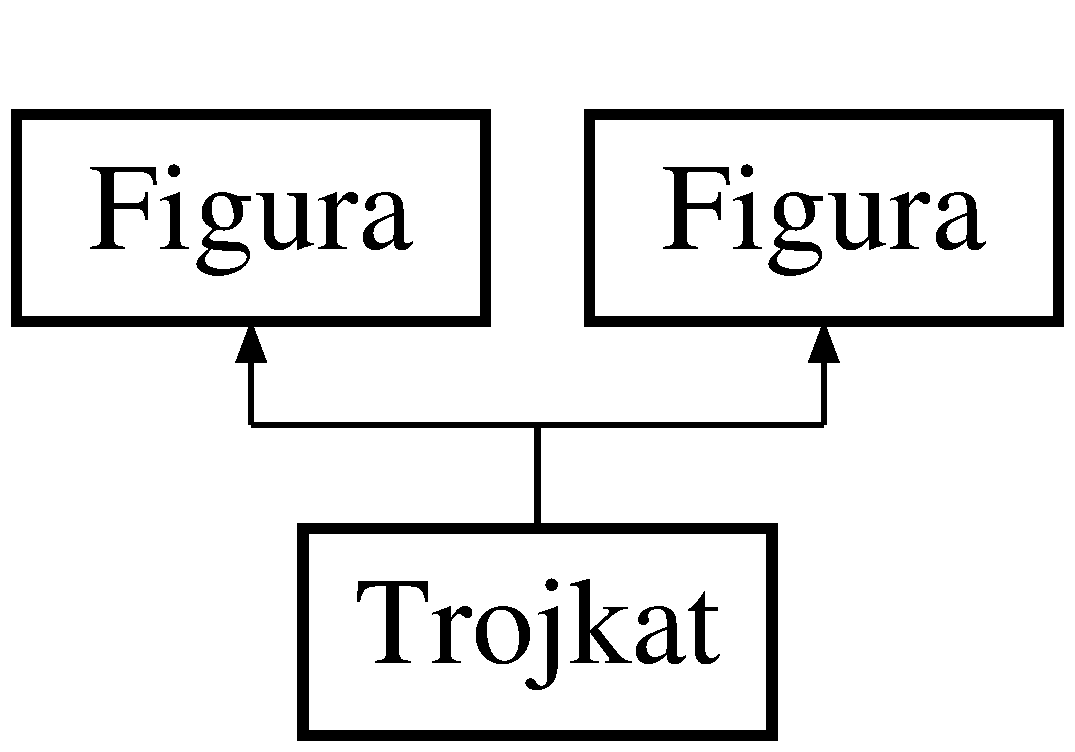
\includegraphics[height=2.000000cm]{classTrojkat}
\end{center}
\end{figure}
\subsection*{Metody publiczne}
\begin{DoxyCompactItemize}
\item 
\hyperlink{classTrojkat_a96b62e4eb4b351234c26b9e8b778c633}{Trojkat} ()
\item 
\hyperlink{classTrojkat_a8a80f197328c308d2ae4816a4d1eefca}{Trojkat} (float x\-\_\-, float y\-\_\-, float a\-\_\-)
\item 
\hyperlink{classTrojkat_acb46695e95bf1d277cda20ca2308dc8f}{$\sim$\-Trojkat} ()
\item 
virtual void \hyperlink{classTrojkat_ac61a9a7c73a7d2b26a006f5d0b93b764}{rysuj} ()
\item 
virtual float \hyperlink{classTrojkat_aaa6d596b67627b3bb7c8262503f4009f}{zwroc\-Rozmiar} ()
\item 
virtual bool \hyperlink{classTrojkat_a871b255c6920fa5310baf3a995b58abc}{czy\-Nalezydo\-Figury} (float \hyperlink{classFigura_ad640a05ebb1ddbf595124f0b31793e8a}{x}, float \hyperlink{classFigura_ab17e5953f2898eb729b2dc506640bce2}{y})
\item 
virtual bool \hyperlink{classTrojkat_a87c603d7ff1eb8dc9fde4918f9913d8c}{czy\-Kolizja} (\hyperlink{classFigura}{Figura} $\ast$druga)
\item 
virtual void \hyperlink{classTrojkat_a87aa9e537564fd357b0a0ed201e31bac}{zmien\-Rozmiar} (float)
\item 
virtual float \hyperlink{classTrojkat_a35e916271aeef83d4ec42001cba75ef7}{zwroc\-Pole} ()
\item 
virtual double \hyperlink{classTrojkat_aba9f0a511f9910617302485b5fae0811}{zwrocodleglosc\-Do\-Kolizji} ()
\item 
virtual void \hyperlink{classTrojkat_a2f6bef37c3aa379f95f5cb1e41cf90ce}{zmien\-Pole} (float)
\item 
virtual int \hyperlink{classTrojkat_af09fa611c1c0fd094883e8a0a9c36b4e}{zwroc\-Typ} ()
\item 
\hyperlink{classTrojkat_a96b62e4eb4b351234c26b9e8b778c633}{Trojkat} ()
\item 
\hyperlink{classTrojkat_a8a80f197328c308d2ae4816a4d1eefca}{Trojkat} (float x\-\_\-, float y\-\_\-, float a\-\_\-)
\item 
\hyperlink{classTrojkat_acb46695e95bf1d277cda20ca2308dc8f}{$\sim$\-Trojkat} ()
\item 
virtual void \hyperlink{classTrojkat_a3d2eaab066fd06a41f275acad39acdeb}{rysuj} ()
\item 
virtual float \hyperlink{classTrojkat_a7a8add838eb57536c3d7d4afa6cf6e9d}{zwroc\-Rozmiar} ()
\item 
virtual bool \hyperlink{classTrojkat_a702583c2fc42a5e250f59de61925be03}{czy\-Nalezydo\-Figury} (float \hyperlink{classFigura_ad640a05ebb1ddbf595124f0b31793e8a}{x}, float \hyperlink{classFigura_ab17e5953f2898eb729b2dc506640bce2}{y})
\item 
virtual bool \hyperlink{classTrojkat_af7a0a4a4ffdc5b832f8c0c933261567e}{czy\-Kolizja} (\hyperlink{classFigura}{Figura} $\ast$druga)
\item 
virtual void \hyperlink{classTrojkat_a8e50af24f4947c6c3b61f4812b0d1ddd}{zmien\-Rozmiar} (float)
\item 
virtual float \hyperlink{classTrojkat_a8437ba74adf44d8724293dfdda0f5c7f}{zwroc\-Pole} ()
\item 
virtual double \hyperlink{classTrojkat_a4ad8638c5afb819d8ab33b9a6b681497}{zwrocodleglosc\-Do\-Kolizji} ()
\item 
virtual void \hyperlink{classTrojkat_a7eeb5a5c810989f3b2790f058c0e3b19}{zmien\-Pole} (float)
\item 
virtual int \hyperlink{classTrojkat_ad00f4b47a0ffc60b9505a3c239e56530}{zwroc\-Typ} ()
\end{DoxyCompactItemize}
\subsection*{Dodatkowe Dziedziczone Składowe}


\subsection{Dokumentacja konstruktora i destruktora}
\hypertarget{classTrojkat_a96b62e4eb4b351234c26b9e8b778c633}{\index{Trojkat@{Trojkat}!Trojkat@{Trojkat}}
\index{Trojkat@{Trojkat}!Trojkat@{Trojkat}}
\subsubsection[{Trojkat}]{\setlength{\rightskip}{0pt plus 5cm}Trojkat\-::\-Trojkat (
\begin{DoxyParamCaption}
{}
\end{DoxyParamCaption}
)}}\label{classTrojkat_a96b62e4eb4b351234c26b9e8b778c633}
\hypertarget{classTrojkat_a8a80f197328c308d2ae4816a4d1eefca}{\index{Trojkat@{Trojkat}!Trojkat@{Trojkat}}
\index{Trojkat@{Trojkat}!Trojkat@{Trojkat}}
\subsubsection[{Trojkat}]{\setlength{\rightskip}{0pt plus 5cm}Trojkat\-::\-Trojkat (
\begin{DoxyParamCaption}
\item[{float}]{x\-\_\-, }
\item[{float}]{y\-\_\-, }
\item[{float}]{a\-\_\-}
\end{DoxyParamCaption}
)}}\label{classTrojkat_a8a80f197328c308d2ae4816a4d1eefca}
\hypertarget{classTrojkat_acb46695e95bf1d277cda20ca2308dc8f}{\index{Trojkat@{Trojkat}!$\sim$\-Trojkat@{$\sim$\-Trojkat}}
\index{$\sim$\-Trojkat@{$\sim$\-Trojkat}!Trojkat@{Trojkat}}
\subsubsection[{$\sim$\-Trojkat}]{\setlength{\rightskip}{0pt plus 5cm}Trojkat\-::$\sim$\-Trojkat (
\begin{DoxyParamCaption}
{}
\end{DoxyParamCaption}
)}}\label{classTrojkat_acb46695e95bf1d277cda20ca2308dc8f}
\hypertarget{classTrojkat_a96b62e4eb4b351234c26b9e8b778c633}{\index{Trojkat@{Trojkat}!Trojkat@{Trojkat}}
\index{Trojkat@{Trojkat}!Trojkat@{Trojkat}}
\subsubsection[{Trojkat}]{\setlength{\rightskip}{0pt plus 5cm}Trojkat\-::\-Trojkat (
\begin{DoxyParamCaption}
{}
\end{DoxyParamCaption}
)}}\label{classTrojkat_a96b62e4eb4b351234c26b9e8b778c633}
\hypertarget{classTrojkat_a8a80f197328c308d2ae4816a4d1eefca}{\index{Trojkat@{Trojkat}!Trojkat@{Trojkat}}
\index{Trojkat@{Trojkat}!Trojkat@{Trojkat}}
\subsubsection[{Trojkat}]{\setlength{\rightskip}{0pt plus 5cm}Trojkat\-::\-Trojkat (
\begin{DoxyParamCaption}
\item[{float}]{x\-\_\-, }
\item[{float}]{y\-\_\-, }
\item[{float}]{a\-\_\-}
\end{DoxyParamCaption}
)}}\label{classTrojkat_a8a80f197328c308d2ae4816a4d1eefca}
\hypertarget{classTrojkat_acb46695e95bf1d277cda20ca2308dc8f}{\index{Trojkat@{Trojkat}!$\sim$\-Trojkat@{$\sim$\-Trojkat}}
\index{$\sim$\-Trojkat@{$\sim$\-Trojkat}!Trojkat@{Trojkat}}
\subsubsection[{$\sim$\-Trojkat}]{\setlength{\rightskip}{0pt plus 5cm}Trojkat\-::$\sim$\-Trojkat (
\begin{DoxyParamCaption}
{}
\end{DoxyParamCaption}
)}}\label{classTrojkat_acb46695e95bf1d277cda20ca2308dc8f}


\subsection{Dokumentacja funkcji składowych}
\hypertarget{classTrojkat_a87c603d7ff1eb8dc9fde4918f9913d8c}{\index{Trojkat@{Trojkat}!czy\-Kolizja@{czy\-Kolizja}}
\index{czy\-Kolizja@{czy\-Kolizja}!Trojkat@{Trojkat}}
\subsubsection[{czy\-Kolizja}]{\setlength{\rightskip}{0pt plus 5cm}bool Trojkat\-::czy\-Kolizja (
\begin{DoxyParamCaption}
\item[{{\bf Figura} $\ast$}]{druga}
\end{DoxyParamCaption}
)\hspace{0.3cm}{\ttfamily [virtual]}}}\label{classTrojkat_a87c603d7ff1eb8dc9fde4918f9913d8c}


Implementuje \hyperlink{classFigura_a7a1cb0014aaaa276f8b17932c394b485}{Figura}.

\hypertarget{classTrojkat_af7a0a4a4ffdc5b832f8c0c933261567e}{\index{Trojkat@{Trojkat}!czy\-Kolizja@{czy\-Kolizja}}
\index{czy\-Kolizja@{czy\-Kolizja}!Trojkat@{Trojkat}}
\subsubsection[{czy\-Kolizja}]{\setlength{\rightskip}{0pt plus 5cm}virtual bool Trojkat\-::czy\-Kolizja (
\begin{DoxyParamCaption}
\item[{{\bf Figura} $\ast$}]{druga}
\end{DoxyParamCaption}
)\hspace{0.3cm}{\ttfamily [virtual]}}}\label{classTrojkat_af7a0a4a4ffdc5b832f8c0c933261567e}


Implementuje \hyperlink{classFigura_a7a1cb0014aaaa276f8b17932c394b485}{Figura}.

\hypertarget{classTrojkat_a871b255c6920fa5310baf3a995b58abc}{\index{Trojkat@{Trojkat}!czy\-Nalezydo\-Figury@{czy\-Nalezydo\-Figury}}
\index{czy\-Nalezydo\-Figury@{czy\-Nalezydo\-Figury}!Trojkat@{Trojkat}}
\subsubsection[{czy\-Nalezydo\-Figury}]{\setlength{\rightskip}{0pt plus 5cm}bool Trojkat\-::czy\-Nalezydo\-Figury (
\begin{DoxyParamCaption}
\item[{float}]{x, }
\item[{float}]{y}
\end{DoxyParamCaption}
)\hspace{0.3cm}{\ttfamily [virtual]}}}\label{classTrojkat_a871b255c6920fa5310baf3a995b58abc}


Implementuje \hyperlink{classFigura_a14f9ba21828b6292488e1fa12bf1b85f}{Figura}.

\hypertarget{classTrojkat_a702583c2fc42a5e250f59de61925be03}{\index{Trojkat@{Trojkat}!czy\-Nalezydo\-Figury@{czy\-Nalezydo\-Figury}}
\index{czy\-Nalezydo\-Figury@{czy\-Nalezydo\-Figury}!Trojkat@{Trojkat}}
\subsubsection[{czy\-Nalezydo\-Figury}]{\setlength{\rightskip}{0pt plus 5cm}virtual bool Trojkat\-::czy\-Nalezydo\-Figury (
\begin{DoxyParamCaption}
\item[{float}]{x, }
\item[{float}]{y}
\end{DoxyParamCaption}
)\hspace{0.3cm}{\ttfamily [virtual]}}}\label{classTrojkat_a702583c2fc42a5e250f59de61925be03}


Implementuje \hyperlink{classFigura_a14f9ba21828b6292488e1fa12bf1b85f}{Figura}.

\hypertarget{classTrojkat_a3d2eaab066fd06a41f275acad39acdeb}{\index{Trojkat@{Trojkat}!rysuj@{rysuj}}
\index{rysuj@{rysuj}!Trojkat@{Trojkat}}
\subsubsection[{rysuj}]{\setlength{\rightskip}{0pt plus 5cm}virtual void Trojkat\-::rysuj (
\begin{DoxyParamCaption}
{}
\end{DoxyParamCaption}
)\hspace{0.3cm}{\ttfamily [virtual]}}}\label{classTrojkat_a3d2eaab066fd06a41f275acad39acdeb}


Implementuje \hyperlink{classFigura_a6ec035fbeb95129af6ca64d2adff7651}{Figura}.

\hypertarget{classTrojkat_ac61a9a7c73a7d2b26a006f5d0b93b764}{\index{Trojkat@{Trojkat}!rysuj@{rysuj}}
\index{rysuj@{rysuj}!Trojkat@{Trojkat}}
\subsubsection[{rysuj}]{\setlength{\rightskip}{0pt plus 5cm}void Trojkat\-::rysuj (
\begin{DoxyParamCaption}
{}
\end{DoxyParamCaption}
)\hspace{0.3cm}{\ttfamily [virtual]}}}\label{classTrojkat_ac61a9a7c73a7d2b26a006f5d0b93b764}


Implementuje \hyperlink{classFigura_a6ec035fbeb95129af6ca64d2adff7651}{Figura}.

\hypertarget{classTrojkat_a2f6bef37c3aa379f95f5cb1e41cf90ce}{\index{Trojkat@{Trojkat}!zmien\-Pole@{zmien\-Pole}}
\index{zmien\-Pole@{zmien\-Pole}!Trojkat@{Trojkat}}
\subsubsection[{zmien\-Pole}]{\setlength{\rightskip}{0pt plus 5cm}void Trojkat\-::zmien\-Pole (
\begin{DoxyParamCaption}
\item[{float}]{dp}
\end{DoxyParamCaption}
)\hspace{0.3cm}{\ttfamily [virtual]}}}\label{classTrojkat_a2f6bef37c3aa379f95f5cb1e41cf90ce}


Implementuje \hyperlink{classFigura_aad1198cc826aa6b3036454fd4f3bb5b3}{Figura}.

\hypertarget{classTrojkat_a7eeb5a5c810989f3b2790f058c0e3b19}{\index{Trojkat@{Trojkat}!zmien\-Pole@{zmien\-Pole}}
\index{zmien\-Pole@{zmien\-Pole}!Trojkat@{Trojkat}}
\subsubsection[{zmien\-Pole}]{\setlength{\rightskip}{0pt plus 5cm}virtual void Trojkat\-::zmien\-Pole (
\begin{DoxyParamCaption}
\item[{float}]{}
\end{DoxyParamCaption}
)\hspace{0.3cm}{\ttfamily [virtual]}}}\label{classTrojkat_a7eeb5a5c810989f3b2790f058c0e3b19}


Implementuje \hyperlink{classFigura_aad1198cc826aa6b3036454fd4f3bb5b3}{Figura}.

\hypertarget{classTrojkat_a87aa9e537564fd357b0a0ed201e31bac}{\index{Trojkat@{Trojkat}!zmien\-Rozmiar@{zmien\-Rozmiar}}
\index{zmien\-Rozmiar@{zmien\-Rozmiar}!Trojkat@{Trojkat}}
\subsubsection[{zmien\-Rozmiar}]{\setlength{\rightskip}{0pt plus 5cm}void Trojkat\-::zmien\-Rozmiar (
\begin{DoxyParamCaption}
\item[{float}]{dr}
\end{DoxyParamCaption}
)\hspace{0.3cm}{\ttfamily [virtual]}}}\label{classTrojkat_a87aa9e537564fd357b0a0ed201e31bac}


Implementuje \hyperlink{classFigura_a7ea2c8b450129878f4347404b8834c6b}{Figura}.

\hypertarget{classTrojkat_a8e50af24f4947c6c3b61f4812b0d1ddd}{\index{Trojkat@{Trojkat}!zmien\-Rozmiar@{zmien\-Rozmiar}}
\index{zmien\-Rozmiar@{zmien\-Rozmiar}!Trojkat@{Trojkat}}
\subsubsection[{zmien\-Rozmiar}]{\setlength{\rightskip}{0pt plus 5cm}virtual void Trojkat\-::zmien\-Rozmiar (
\begin{DoxyParamCaption}
\item[{float}]{}
\end{DoxyParamCaption}
)\hspace{0.3cm}{\ttfamily [virtual]}}}\label{classTrojkat_a8e50af24f4947c6c3b61f4812b0d1ddd}


Implementuje \hyperlink{classFigura_a7ea2c8b450129878f4347404b8834c6b}{Figura}.

\hypertarget{classTrojkat_a4ad8638c5afb819d8ab33b9a6b681497}{\index{Trojkat@{Trojkat}!zwrocodleglosc\-Do\-Kolizji@{zwrocodleglosc\-Do\-Kolizji}}
\index{zwrocodleglosc\-Do\-Kolizji@{zwrocodleglosc\-Do\-Kolizji}!Trojkat@{Trojkat}}
\subsubsection[{zwrocodleglosc\-Do\-Kolizji}]{\setlength{\rightskip}{0pt plus 5cm}virtual double Trojkat\-::zwrocodleglosc\-Do\-Kolizji (
\begin{DoxyParamCaption}
{}
\end{DoxyParamCaption}
)\hspace{0.3cm}{\ttfamily [virtual]}}}\label{classTrojkat_a4ad8638c5afb819d8ab33b9a6b681497}


Implementuje \hyperlink{classFigura_a3e534b43a279aeec36c5b28ac731e0f8}{Figura}.

\hypertarget{classTrojkat_aba9f0a511f9910617302485b5fae0811}{\index{Trojkat@{Trojkat}!zwrocodleglosc\-Do\-Kolizji@{zwrocodleglosc\-Do\-Kolizji}}
\index{zwrocodleglosc\-Do\-Kolizji@{zwrocodleglosc\-Do\-Kolizji}!Trojkat@{Trojkat}}
\subsubsection[{zwrocodleglosc\-Do\-Kolizji}]{\setlength{\rightskip}{0pt plus 5cm}double Trojkat\-::zwrocodleglosc\-Do\-Kolizji (
\begin{DoxyParamCaption}
{}
\end{DoxyParamCaption}
)\hspace{0.3cm}{\ttfamily [virtual]}}}\label{classTrojkat_aba9f0a511f9910617302485b5fae0811}


Implementuje \hyperlink{classFigura_a3e534b43a279aeec36c5b28ac731e0f8}{Figura}.

\hypertarget{classTrojkat_a8437ba74adf44d8724293dfdda0f5c7f}{\index{Trojkat@{Trojkat}!zwroc\-Pole@{zwroc\-Pole}}
\index{zwroc\-Pole@{zwroc\-Pole}!Trojkat@{Trojkat}}
\subsubsection[{zwroc\-Pole}]{\setlength{\rightskip}{0pt plus 5cm}virtual float Trojkat\-::zwroc\-Pole (
\begin{DoxyParamCaption}
{}
\end{DoxyParamCaption}
)\hspace{0.3cm}{\ttfamily [virtual]}}}\label{classTrojkat_a8437ba74adf44d8724293dfdda0f5c7f}


Implementuje \hyperlink{classFigura_a78861f3fce7e615ba30b47aa1cdcebec}{Figura}.

\hypertarget{classTrojkat_a35e916271aeef83d4ec42001cba75ef7}{\index{Trojkat@{Trojkat}!zwroc\-Pole@{zwroc\-Pole}}
\index{zwroc\-Pole@{zwroc\-Pole}!Trojkat@{Trojkat}}
\subsubsection[{zwroc\-Pole}]{\setlength{\rightskip}{0pt plus 5cm}float Trojkat\-::zwroc\-Pole (
\begin{DoxyParamCaption}
{}
\end{DoxyParamCaption}
)\hspace{0.3cm}{\ttfamily [virtual]}}}\label{classTrojkat_a35e916271aeef83d4ec42001cba75ef7}


Implementuje \hyperlink{classFigura_a78861f3fce7e615ba30b47aa1cdcebec}{Figura}.

\hypertarget{classTrojkat_a7a8add838eb57536c3d7d4afa6cf6e9d}{\index{Trojkat@{Trojkat}!zwroc\-Rozmiar@{zwroc\-Rozmiar}}
\index{zwroc\-Rozmiar@{zwroc\-Rozmiar}!Trojkat@{Trojkat}}
\subsubsection[{zwroc\-Rozmiar}]{\setlength{\rightskip}{0pt plus 5cm}virtual float Trojkat\-::zwroc\-Rozmiar (
\begin{DoxyParamCaption}
{}
\end{DoxyParamCaption}
)\hspace{0.3cm}{\ttfamily [virtual]}}}\label{classTrojkat_a7a8add838eb57536c3d7d4afa6cf6e9d}


Implementuje \hyperlink{classFigura_aaeb587028aafd028e134079c249b0c88}{Figura}.

\hypertarget{classTrojkat_aaa6d596b67627b3bb7c8262503f4009f}{\index{Trojkat@{Trojkat}!zwroc\-Rozmiar@{zwroc\-Rozmiar}}
\index{zwroc\-Rozmiar@{zwroc\-Rozmiar}!Trojkat@{Trojkat}}
\subsubsection[{zwroc\-Rozmiar}]{\setlength{\rightskip}{0pt plus 5cm}float Trojkat\-::zwroc\-Rozmiar (
\begin{DoxyParamCaption}
{}
\end{DoxyParamCaption}
)\hspace{0.3cm}{\ttfamily [virtual]}}}\label{classTrojkat_aaa6d596b67627b3bb7c8262503f4009f}


Implementuje \hyperlink{classFigura_aaeb587028aafd028e134079c249b0c88}{Figura}.

\hypertarget{classTrojkat_ad00f4b47a0ffc60b9505a3c239e56530}{\index{Trojkat@{Trojkat}!zwroc\-Typ@{zwroc\-Typ}}
\index{zwroc\-Typ@{zwroc\-Typ}!Trojkat@{Trojkat}}
\subsubsection[{zwroc\-Typ}]{\setlength{\rightskip}{0pt plus 5cm}virtual int Trojkat\-::zwroc\-Typ (
\begin{DoxyParamCaption}
{}
\end{DoxyParamCaption}
)\hspace{0.3cm}{\ttfamily [virtual]}}}\label{classTrojkat_ad00f4b47a0ffc60b9505a3c239e56530}


Implementuje \hyperlink{classFigura_ab04732de63f17d4c3776990d24897db7}{Figura}.

\hypertarget{classTrojkat_af09fa611c1c0fd094883e8a0a9c36b4e}{\index{Trojkat@{Trojkat}!zwroc\-Typ@{zwroc\-Typ}}
\index{zwroc\-Typ@{zwroc\-Typ}!Trojkat@{Trojkat}}
\subsubsection[{zwroc\-Typ}]{\setlength{\rightskip}{0pt plus 5cm}int Trojkat\-::zwroc\-Typ (
\begin{DoxyParamCaption}
{}
\end{DoxyParamCaption}
)\hspace{0.3cm}{\ttfamily [virtual]}}}\label{classTrojkat_af09fa611c1c0fd094883e8a0a9c36b4e}


Implementuje \hyperlink{classFigura_ab04732de63f17d4c3776990d24897db7}{Figura}.



Dokumentacja dla tej klasy została wygenerowana z plików\-:\begin{DoxyCompactItemize}
\item 
Gra\-Figury/\hyperlink{GraFigury_2trojkat_8h}{trojkat.\-h}\item 
Gra\-Figury/\hyperlink{GraFigury_2trojkat_8cpp}{trojkat.\-cpp}\end{DoxyCompactItemize}

\hypertarget{classUi__Dialog}{\section{Dokumentacja klasy Ui\-\_\-\-Dialog}
\label{classUi__Dialog}\index{Ui\-\_\-\-Dialog@{Ui\-\_\-\-Dialog}}
}


{\ttfamily \#include $<$ui\-\_\-dialog.\-h$>$}

Diagram dziedziczenia dla Ui\-\_\-\-Dialog\begin{figure}[H]
\begin{center}
\leavevmode
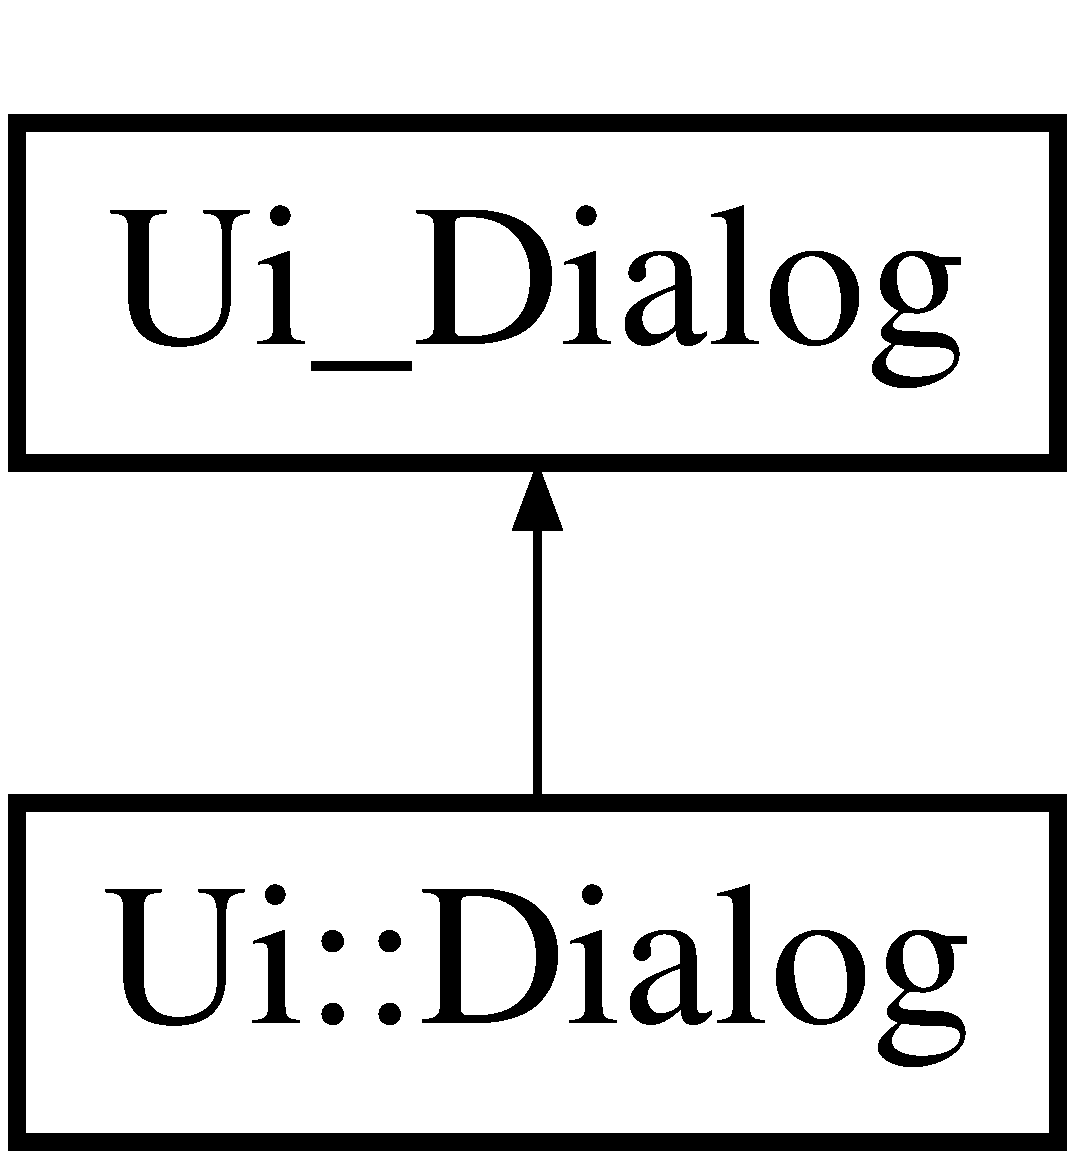
\includegraphics[height=2.000000cm]{classUi__Dialog}
\end{center}
\end{figure}
\subsection*{Metody publiczne}
\begin{DoxyCompactItemize}
\item 
void \hyperlink{classUi__Dialog_a4f6a478c3ecdafabffb17b39cb26444a}{setup\-Ui} (Q\-Dialog $\ast$\hyperlink{classDialog}{Dialog})
\item 
void \hyperlink{classUi__Dialog_afa0ccb6f716ca6178260522a193c250e}{retranslate\-Ui} (Q\-Dialog $\ast$\hyperlink{classDialog}{Dialog})
\end{DoxyCompactItemize}
\subsection*{Atrybuty publiczne}
\begin{DoxyCompactItemize}
\item 
Q\-Widget $\ast$ \hyperlink{classUi__Dialog_a4a01239907c0d25e55efbe5811d64e94}{horizontal\-Layout\-Widget\-\_\-2}
\item 
Q\-H\-Box\-Layout $\ast$ \hyperlink{classUi__Dialog_a289b49bcdd28408efe2510f029535c2b}{horizontal\-Layout\-\_\-2}
\item 
Q\-Line\-Edit $\ast$ \hyperlink{classUi__Dialog_ab46d172e983ee875ea7d404f0e9cffeb}{line\-Edit\-I\-P}
\item 
Q\-Line\-Edit $\ast$ \hyperlink{classUi__Dialog_af72591b169533ffca5bfb1aef6771696}{line\-Edit\-Port}
\item 
Q\-Push\-Button $\ast$ \hyperlink{classUi__Dialog_a80234b371a2b143b74be0c4351ad2267}{push\-Button\-Polacz}
\item 
Q\-Line\-Edit $\ast$ \hyperlink{classUi__Dialog_a934cf16b9b36614a93f04261c652c1c7}{line\-Edit}
\end{DoxyCompactItemize}


\subsection{Dokumentacja funkcji składowych}
\hypertarget{classUi__Dialog_afa0ccb6f716ca6178260522a193c250e}{\index{Ui\-\_\-\-Dialog@{Ui\-\_\-\-Dialog}!retranslate\-Ui@{retranslate\-Ui}}
\index{retranslate\-Ui@{retranslate\-Ui}!Ui_Dialog@{Ui\-\_\-\-Dialog}}
\subsubsection[{retranslate\-Ui}]{\setlength{\rightskip}{0pt plus 5cm}void Ui\-\_\-\-Dialog\-::retranslate\-Ui (
\begin{DoxyParamCaption}
\item[{Q\-Dialog $\ast$}]{Dialog}
\end{DoxyParamCaption}
)\hspace{0.3cm}{\ttfamily [inline]}}}\label{classUi__Dialog_afa0ccb6f716ca6178260522a193c250e}
\hypertarget{classUi__Dialog_a4f6a478c3ecdafabffb17b39cb26444a}{\index{Ui\-\_\-\-Dialog@{Ui\-\_\-\-Dialog}!setup\-Ui@{setup\-Ui}}
\index{setup\-Ui@{setup\-Ui}!Ui_Dialog@{Ui\-\_\-\-Dialog}}
\subsubsection[{setup\-Ui}]{\setlength{\rightskip}{0pt plus 5cm}void Ui\-\_\-\-Dialog\-::setup\-Ui (
\begin{DoxyParamCaption}
\item[{Q\-Dialog $\ast$}]{Dialog}
\end{DoxyParamCaption}
)\hspace{0.3cm}{\ttfamily [inline]}}}\label{classUi__Dialog_a4f6a478c3ecdafabffb17b39cb26444a}


\subsection{Dokumentacja atrybutów składowych}
\hypertarget{classUi__Dialog_a289b49bcdd28408efe2510f029535c2b}{\index{Ui\-\_\-\-Dialog@{Ui\-\_\-\-Dialog}!horizontal\-Layout\-\_\-2@{horizontal\-Layout\-\_\-2}}
\index{horizontal\-Layout\-\_\-2@{horizontal\-Layout\-\_\-2}!Ui_Dialog@{Ui\-\_\-\-Dialog}}
\subsubsection[{horizontal\-Layout\-\_\-2}]{\setlength{\rightskip}{0pt plus 5cm}Q\-H\-Box\-Layout$\ast$ Ui\-\_\-\-Dialog\-::horizontal\-Layout\-\_\-2}}\label{classUi__Dialog_a289b49bcdd28408efe2510f029535c2b}
\hypertarget{classUi__Dialog_a4a01239907c0d25e55efbe5811d64e94}{\index{Ui\-\_\-\-Dialog@{Ui\-\_\-\-Dialog}!horizontal\-Layout\-Widget\-\_\-2@{horizontal\-Layout\-Widget\-\_\-2}}
\index{horizontal\-Layout\-Widget\-\_\-2@{horizontal\-Layout\-Widget\-\_\-2}!Ui_Dialog@{Ui\-\_\-\-Dialog}}
\subsubsection[{horizontal\-Layout\-Widget\-\_\-2}]{\setlength{\rightskip}{0pt plus 5cm}Q\-Widget$\ast$ Ui\-\_\-\-Dialog\-::horizontal\-Layout\-Widget\-\_\-2}}\label{classUi__Dialog_a4a01239907c0d25e55efbe5811d64e94}
\hypertarget{classUi__Dialog_a934cf16b9b36614a93f04261c652c1c7}{\index{Ui\-\_\-\-Dialog@{Ui\-\_\-\-Dialog}!line\-Edit@{line\-Edit}}
\index{line\-Edit@{line\-Edit}!Ui_Dialog@{Ui\-\_\-\-Dialog}}
\subsubsection[{line\-Edit}]{\setlength{\rightskip}{0pt plus 5cm}Q\-Line\-Edit$\ast$ Ui\-\_\-\-Dialog\-::line\-Edit}}\label{classUi__Dialog_a934cf16b9b36614a93f04261c652c1c7}
\hypertarget{classUi__Dialog_ab46d172e983ee875ea7d404f0e9cffeb}{\index{Ui\-\_\-\-Dialog@{Ui\-\_\-\-Dialog}!line\-Edit\-I\-P@{line\-Edit\-I\-P}}
\index{line\-Edit\-I\-P@{line\-Edit\-I\-P}!Ui_Dialog@{Ui\-\_\-\-Dialog}}
\subsubsection[{line\-Edit\-I\-P}]{\setlength{\rightskip}{0pt plus 5cm}Q\-Line\-Edit$\ast$ Ui\-\_\-\-Dialog\-::line\-Edit\-I\-P}}\label{classUi__Dialog_ab46d172e983ee875ea7d404f0e9cffeb}
\hypertarget{classUi__Dialog_af72591b169533ffca5bfb1aef6771696}{\index{Ui\-\_\-\-Dialog@{Ui\-\_\-\-Dialog}!line\-Edit\-Port@{line\-Edit\-Port}}
\index{line\-Edit\-Port@{line\-Edit\-Port}!Ui_Dialog@{Ui\-\_\-\-Dialog}}
\subsubsection[{line\-Edit\-Port}]{\setlength{\rightskip}{0pt plus 5cm}Q\-Line\-Edit$\ast$ Ui\-\_\-\-Dialog\-::line\-Edit\-Port}}\label{classUi__Dialog_af72591b169533ffca5bfb1aef6771696}
\hypertarget{classUi__Dialog_a80234b371a2b143b74be0c4351ad2267}{\index{Ui\-\_\-\-Dialog@{Ui\-\_\-\-Dialog}!push\-Button\-Polacz@{push\-Button\-Polacz}}
\index{push\-Button\-Polacz@{push\-Button\-Polacz}!Ui_Dialog@{Ui\-\_\-\-Dialog}}
\subsubsection[{push\-Button\-Polacz}]{\setlength{\rightskip}{0pt plus 5cm}Q\-Push\-Button$\ast$ Ui\-\_\-\-Dialog\-::push\-Button\-Polacz}}\label{classUi__Dialog_a80234b371a2b143b74be0c4351ad2267}


Dokumentacja dla tej klasy została wygenerowana z pliku\-:\begin{DoxyCompactItemize}
\item 
Gra\-Figury/\hyperlink{ui__dialog_8h}{ui\-\_\-dialog.\-h}\end{DoxyCompactItemize}

\hypertarget{classUi__Dialog2}{\section{Dokumentacja klasy Ui\-\_\-\-Dialog2}
\label{classUi__Dialog2}\index{Ui\-\_\-\-Dialog2@{Ui\-\_\-\-Dialog2}}
}


{\ttfamily \#include $<$ui\-\_\-dialog2.\-h$>$}

Diagram dziedziczenia dla Ui\-\_\-\-Dialog2\begin{figure}[H]
\begin{center}
\leavevmode
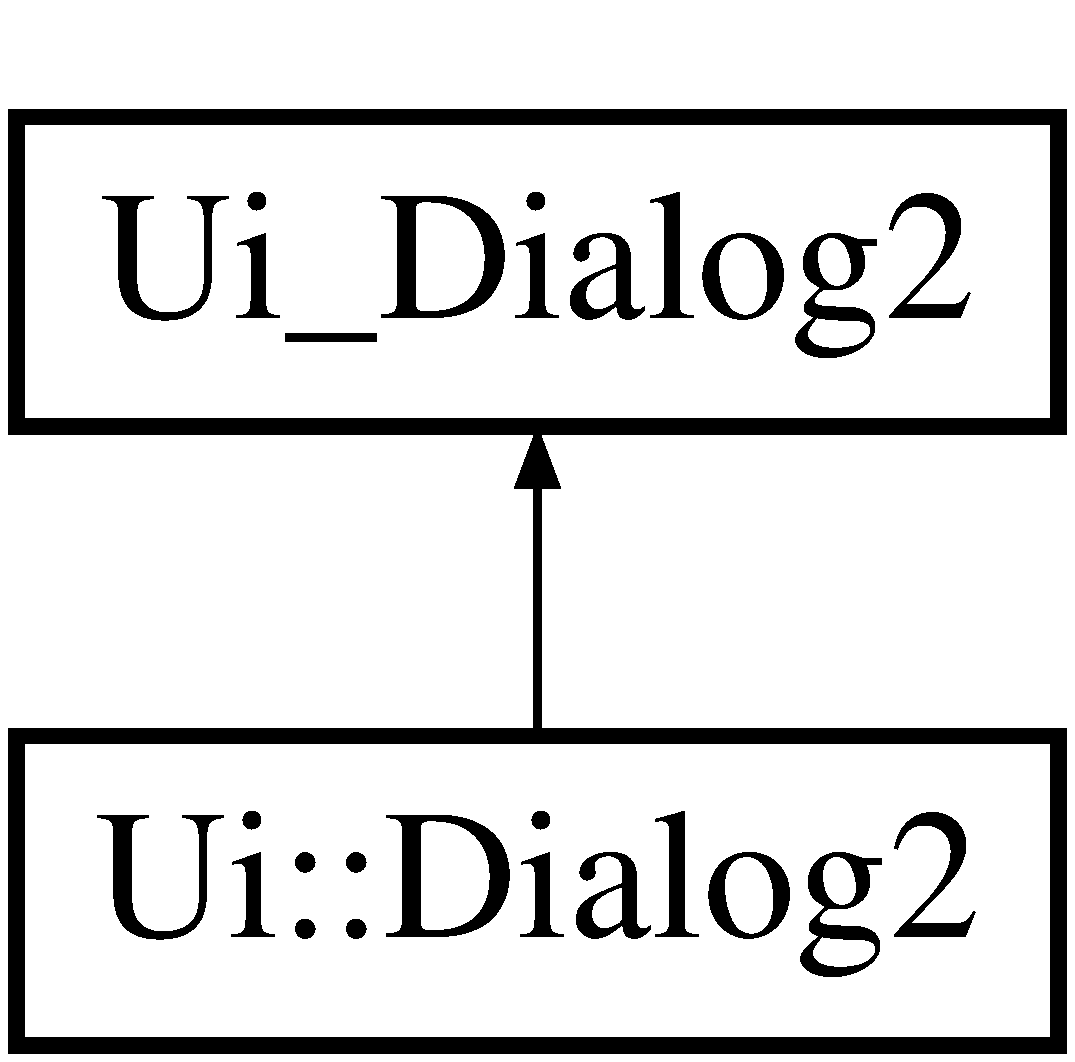
\includegraphics[height=2.000000cm]{classUi__Dialog2}
\end{center}
\end{figure}
\subsection*{Metody publiczne}
\begin{DoxyCompactItemize}
\item 
void \hyperlink{classUi__Dialog2_a6844bf81dbbb01d6eb47136862dccaa8}{setup\-Ui} (Q\-Dialog $\ast$\hyperlink{classDialog2}{Dialog2})
\item 
void \hyperlink{classUi__Dialog2_a26d6371581ce3b88c8814129a6bdc607}{retranslate\-Ui} (Q\-Dialog $\ast$\hyperlink{classDialog2}{Dialog2})
\end{DoxyCompactItemize}
\subsection*{Atrybuty publiczne}
\begin{DoxyCompactItemize}
\item 
Q\-Label $\ast$ \hyperlink{classUi__Dialog2_a8dbc9bc2d13fc587b1013a6fea211419}{label}
\item 
Q\-Push\-Button $\ast$ \hyperlink{classUi__Dialog2_a02fa58cd4b3b9c0e32a192c4178899e1}{push\-Button\-\_\-2}
\end{DoxyCompactItemize}


\subsection{Dokumentacja funkcji składowych}
\hypertarget{classUi__Dialog2_a26d6371581ce3b88c8814129a6bdc607}{\index{Ui\-\_\-\-Dialog2@{Ui\-\_\-\-Dialog2}!retranslate\-Ui@{retranslate\-Ui}}
\index{retranslate\-Ui@{retranslate\-Ui}!Ui_Dialog2@{Ui\-\_\-\-Dialog2}}
\subsubsection[{retranslate\-Ui}]{\setlength{\rightskip}{0pt plus 5cm}void Ui\-\_\-\-Dialog2\-::retranslate\-Ui (
\begin{DoxyParamCaption}
\item[{Q\-Dialog $\ast$}]{Dialog2}
\end{DoxyParamCaption}
)\hspace{0.3cm}{\ttfamily [inline]}}}\label{classUi__Dialog2_a26d6371581ce3b88c8814129a6bdc607}
\hypertarget{classUi__Dialog2_a6844bf81dbbb01d6eb47136862dccaa8}{\index{Ui\-\_\-\-Dialog2@{Ui\-\_\-\-Dialog2}!setup\-Ui@{setup\-Ui}}
\index{setup\-Ui@{setup\-Ui}!Ui_Dialog2@{Ui\-\_\-\-Dialog2}}
\subsubsection[{setup\-Ui}]{\setlength{\rightskip}{0pt plus 5cm}void Ui\-\_\-\-Dialog2\-::setup\-Ui (
\begin{DoxyParamCaption}
\item[{Q\-Dialog $\ast$}]{Dialog2}
\end{DoxyParamCaption}
)\hspace{0.3cm}{\ttfamily [inline]}}}\label{classUi__Dialog2_a6844bf81dbbb01d6eb47136862dccaa8}


\subsection{Dokumentacja atrybutów składowych}
\hypertarget{classUi__Dialog2_a8dbc9bc2d13fc587b1013a6fea211419}{\index{Ui\-\_\-\-Dialog2@{Ui\-\_\-\-Dialog2}!label@{label}}
\index{label@{label}!Ui_Dialog2@{Ui\-\_\-\-Dialog2}}
\subsubsection[{label}]{\setlength{\rightskip}{0pt plus 5cm}Q\-Label$\ast$ Ui\-\_\-\-Dialog2\-::label}}\label{classUi__Dialog2_a8dbc9bc2d13fc587b1013a6fea211419}
\hypertarget{classUi__Dialog2_a02fa58cd4b3b9c0e32a192c4178899e1}{\index{Ui\-\_\-\-Dialog2@{Ui\-\_\-\-Dialog2}!push\-Button\-\_\-2@{push\-Button\-\_\-2}}
\index{push\-Button\-\_\-2@{push\-Button\-\_\-2}!Ui_Dialog2@{Ui\-\_\-\-Dialog2}}
\subsubsection[{push\-Button\-\_\-2}]{\setlength{\rightskip}{0pt plus 5cm}Q\-Push\-Button$\ast$ Ui\-\_\-\-Dialog2\-::push\-Button\-\_\-2}}\label{classUi__Dialog2_a02fa58cd4b3b9c0e32a192c4178899e1}


Dokumentacja dla tej klasy została wygenerowana z pliku\-:\begin{DoxyCompactItemize}
\item 
Gra\-Figury/\hyperlink{ui__dialog2_8h}{ui\-\_\-dialog2.\-h}\end{DoxyCompactItemize}

\hypertarget{classUi__MainWindow}{\section{Dokumentacja klasy Ui\-\_\-\-Main\-Window}
\label{classUi__MainWindow}\index{Ui\-\_\-\-Main\-Window@{Ui\-\_\-\-Main\-Window}}
}


{\ttfamily \#include $<$ui\-\_\-mainwindow.\-h$>$}

Diagram dziedziczenia dla Ui\-\_\-\-Main\-Window\begin{figure}[H]
\begin{center}
\leavevmode
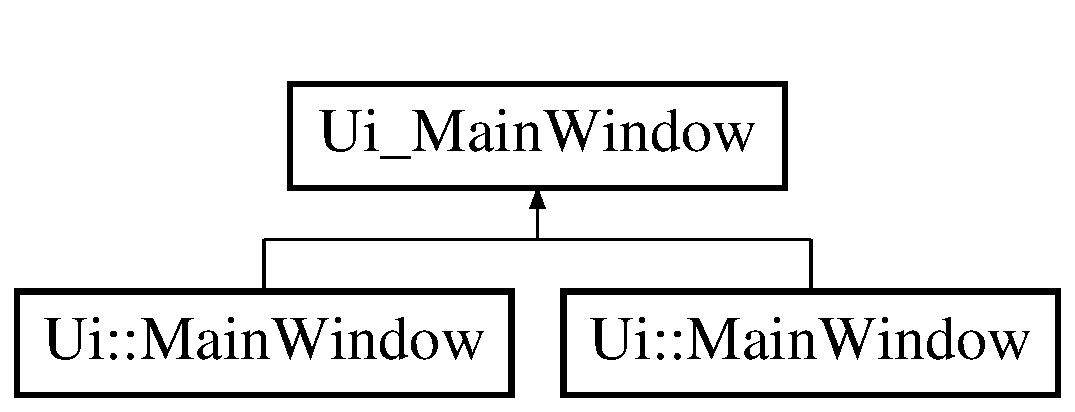
\includegraphics[height=2.000000cm]{d5/d3f/classUi__MainWindow}
\end{center}
\end{figure}
\subsection*{Metody publiczne}
\begin{DoxyCompactItemize}
\item 
void \hyperlink{classUi__MainWindow_acf4a0872c4c77d8f43a2ec66ed849b58}{setup\-Ui} (Q\-Main\-Window $\ast$\hyperlink{classMainWindow}{Main\-Window})
\item 
void \hyperlink{classUi__MainWindow_a097dd160c3534a204904cb374412c618}{retranslate\-Ui} (Q\-Main\-Window $\ast$\hyperlink{classMainWindow}{Main\-Window})
\item 
void \hyperlink{classUi__MainWindow_acf4a0872c4c77d8f43a2ec66ed849b58}{setup\-Ui} (Q\-Main\-Window $\ast$\hyperlink{classMainWindow}{Main\-Window})
\item 
void \hyperlink{classUi__MainWindow_a097dd160c3534a204904cb374412c618}{retranslate\-Ui} (Q\-Main\-Window $\ast$\hyperlink{classMainWindow}{Main\-Window})
\end{DoxyCompactItemize}
\subsection*{Atrybuty publiczne}
\begin{DoxyCompactItemize}
\item 
Q\-Widget $\ast$ \hyperlink{classUi__MainWindow_a6600dd3bdd3d55e535659e4a4096ea48}{central\-Widget}
\item 
\hyperlink{classMyGLWidget}{My\-G\-L\-Widget} $\ast$ \hyperlink{classUi__MainWindow_a53bd42b7570ff9a0e4529859b6551a28}{widget}
\item 
Q\-Push\-Button $\ast$ \hyperlink{classUi__MainWindow_ac1c64d26e7ebcb1aadce071550e18da6}{push\-Button\-Polacz}
\item 
Q\-Label $\ast$ \hyperlink{classUi__MainWindow_adc1b943d721ebbdfb47027d194902d43}{label\-Wynik1}
\item 
Q\-Label $\ast$ \hyperlink{classUi__MainWindow_abd47404a5d7fcad65beab8bd5cbe326d}{label\-Wynik}
\item 
Q\-Status\-Bar $\ast$ \hyperlink{classUi__MainWindow_afa919f3af6f2f526a70f1fa331f63724}{status\-Bar}
\item 
Q\-Widget $\ast$ \hyperlink{classUi__MainWindow_a805d415fff07a22a85219e1f22f2da28}{vertical\-Layout\-Widget}
\item 
Q\-V\-Box\-Layout $\ast$ \hyperlink{classUi__MainWindow_aecd96a04789fcfec3f98d80390ad8184}{vertical\-Layout}
\item 
Q\-H\-Box\-Layout $\ast$ \hyperlink{classUi__MainWindow_acd6fdc9ebacc4b25b834162380d75ce8}{horizontal\-Layout}
\item 
Q\-Line\-Edit $\ast$ \hyperlink{classUi__MainWindow_a6637c5ffd655e9860bc45cc7214a8405}{line\-Edit\-Server}
\item 
Q\-Combo\-Box $\ast$ \hyperlink{classUi__MainWindow_af4df84479fcdbcc4c6d2d3e39046317a}{combo\-Box}
\item 
Q\-Push\-Button $\ast$ \hyperlink{classUi__MainWindow_ab56041a4b9969302779f37709ec2aa32}{push\-Button\-Start}
\item 
Q\-Push\-Button $\ast$ \hyperlink{classUi__MainWindow_a7ffebcd872c64954df2f113b5c5a40c4}{push\-Button\-Stop}
\item 
Q\-Label $\ast$ \hyperlink{classUi__MainWindow_a6e626afc4541c9a658e3164a89d10eb3}{label\-I\-P}
\item 
Q\-Label $\ast$ \hyperlink{classUi__MainWindow_a5b07c23cfb9e49ae640e58c604d3e118}{label\-Port}
\end{DoxyCompactItemize}


\subsection{Dokumentacja funkcji składowych}
\hypertarget{classUi__MainWindow_a097dd160c3534a204904cb374412c618}{\index{Ui\-\_\-\-Main\-Window@{Ui\-\_\-\-Main\-Window}!retranslate\-Ui@{retranslate\-Ui}}
\index{retranslate\-Ui@{retranslate\-Ui}!Ui_MainWindow@{Ui\-\_\-\-Main\-Window}}
\subsubsection[{retranslate\-Ui}]{\setlength{\rightskip}{0pt plus 5cm}void Ui\-\_\-\-Main\-Window\-::retranslate\-Ui (
\begin{DoxyParamCaption}
\item[{Q\-Main\-Window $\ast$}]{Main\-Window}
\end{DoxyParamCaption}
)\hspace{0.3cm}{\ttfamily [inline]}}}\label{classUi__MainWindow_a097dd160c3534a204904cb374412c618}
\hypertarget{classUi__MainWindow_a097dd160c3534a204904cb374412c618}{\index{Ui\-\_\-\-Main\-Window@{Ui\-\_\-\-Main\-Window}!retranslate\-Ui@{retranslate\-Ui}}
\index{retranslate\-Ui@{retranslate\-Ui}!Ui_MainWindow@{Ui\-\_\-\-Main\-Window}}
\subsubsection[{retranslate\-Ui}]{\setlength{\rightskip}{0pt plus 5cm}void Ui\-\_\-\-Main\-Window\-::retranslate\-Ui (
\begin{DoxyParamCaption}
\item[{Q\-Main\-Window $\ast$}]{Main\-Window}
\end{DoxyParamCaption}
)\hspace{0.3cm}{\ttfamily [inline]}}}\label{classUi__MainWindow_a097dd160c3534a204904cb374412c618}
\hypertarget{classUi__MainWindow_acf4a0872c4c77d8f43a2ec66ed849b58}{\index{Ui\-\_\-\-Main\-Window@{Ui\-\_\-\-Main\-Window}!setup\-Ui@{setup\-Ui}}
\index{setup\-Ui@{setup\-Ui}!Ui_MainWindow@{Ui\-\_\-\-Main\-Window}}
\subsubsection[{setup\-Ui}]{\setlength{\rightskip}{0pt plus 5cm}void Ui\-\_\-\-Main\-Window\-::setup\-Ui (
\begin{DoxyParamCaption}
\item[{Q\-Main\-Window $\ast$}]{Main\-Window}
\end{DoxyParamCaption}
)\hspace{0.3cm}{\ttfamily [inline]}}}\label{classUi__MainWindow_acf4a0872c4c77d8f43a2ec66ed849b58}
\hypertarget{classUi__MainWindow_acf4a0872c4c77d8f43a2ec66ed849b58}{\index{Ui\-\_\-\-Main\-Window@{Ui\-\_\-\-Main\-Window}!setup\-Ui@{setup\-Ui}}
\index{setup\-Ui@{setup\-Ui}!Ui_MainWindow@{Ui\-\_\-\-Main\-Window}}
\subsubsection[{setup\-Ui}]{\setlength{\rightskip}{0pt plus 5cm}void Ui\-\_\-\-Main\-Window\-::setup\-Ui (
\begin{DoxyParamCaption}
\item[{Q\-Main\-Window $\ast$}]{Main\-Window}
\end{DoxyParamCaption}
)\hspace{0.3cm}{\ttfamily [inline]}}}\label{classUi__MainWindow_acf4a0872c4c77d8f43a2ec66ed849b58}


\subsection{Dokumentacja atrybutów składowych}
\hypertarget{classUi__MainWindow_a6600dd3bdd3d55e535659e4a4096ea48}{\index{Ui\-\_\-\-Main\-Window@{Ui\-\_\-\-Main\-Window}!central\-Widget@{central\-Widget}}
\index{central\-Widget@{central\-Widget}!Ui_MainWindow@{Ui\-\_\-\-Main\-Window}}
\subsubsection[{central\-Widget}]{\setlength{\rightskip}{0pt plus 5cm}Q\-Widget $\ast$ Ui\-\_\-\-Main\-Window\-::central\-Widget}}\label{classUi__MainWindow_a6600dd3bdd3d55e535659e4a4096ea48}
\hypertarget{classUi__MainWindow_af4df84479fcdbcc4c6d2d3e39046317a}{\index{Ui\-\_\-\-Main\-Window@{Ui\-\_\-\-Main\-Window}!combo\-Box@{combo\-Box}}
\index{combo\-Box@{combo\-Box}!Ui_MainWindow@{Ui\-\_\-\-Main\-Window}}
\subsubsection[{combo\-Box}]{\setlength{\rightskip}{0pt plus 5cm}Q\-Combo\-Box$\ast$ Ui\-\_\-\-Main\-Window\-::combo\-Box}}\label{classUi__MainWindow_af4df84479fcdbcc4c6d2d3e39046317a}
\hypertarget{classUi__MainWindow_acd6fdc9ebacc4b25b834162380d75ce8}{\index{Ui\-\_\-\-Main\-Window@{Ui\-\_\-\-Main\-Window}!horizontal\-Layout@{horizontal\-Layout}}
\index{horizontal\-Layout@{horizontal\-Layout}!Ui_MainWindow@{Ui\-\_\-\-Main\-Window}}
\subsubsection[{horizontal\-Layout}]{\setlength{\rightskip}{0pt plus 5cm}Q\-H\-Box\-Layout$\ast$ Ui\-\_\-\-Main\-Window\-::horizontal\-Layout}}\label{classUi__MainWindow_acd6fdc9ebacc4b25b834162380d75ce8}
\hypertarget{classUi__MainWindow_a6e626afc4541c9a658e3164a89d10eb3}{\index{Ui\-\_\-\-Main\-Window@{Ui\-\_\-\-Main\-Window}!label\-I\-P@{label\-I\-P}}
\index{label\-I\-P@{label\-I\-P}!Ui_MainWindow@{Ui\-\_\-\-Main\-Window}}
\subsubsection[{label\-I\-P}]{\setlength{\rightskip}{0pt plus 5cm}Q\-Label$\ast$ Ui\-\_\-\-Main\-Window\-::label\-I\-P}}\label{classUi__MainWindow_a6e626afc4541c9a658e3164a89d10eb3}
\hypertarget{classUi__MainWindow_a5b07c23cfb9e49ae640e58c604d3e118}{\index{Ui\-\_\-\-Main\-Window@{Ui\-\_\-\-Main\-Window}!label\-Port@{label\-Port}}
\index{label\-Port@{label\-Port}!Ui_MainWindow@{Ui\-\_\-\-Main\-Window}}
\subsubsection[{label\-Port}]{\setlength{\rightskip}{0pt plus 5cm}Q\-Label$\ast$ Ui\-\_\-\-Main\-Window\-::label\-Port}}\label{classUi__MainWindow_a5b07c23cfb9e49ae640e58c604d3e118}
\hypertarget{classUi__MainWindow_abd47404a5d7fcad65beab8bd5cbe326d}{\index{Ui\-\_\-\-Main\-Window@{Ui\-\_\-\-Main\-Window}!label\-Wynik@{label\-Wynik}}
\index{label\-Wynik@{label\-Wynik}!Ui_MainWindow@{Ui\-\_\-\-Main\-Window}}
\subsubsection[{label\-Wynik}]{\setlength{\rightskip}{0pt plus 5cm}Q\-Label$\ast$ Ui\-\_\-\-Main\-Window\-::label\-Wynik}}\label{classUi__MainWindow_abd47404a5d7fcad65beab8bd5cbe326d}
\hypertarget{classUi__MainWindow_adc1b943d721ebbdfb47027d194902d43}{\index{Ui\-\_\-\-Main\-Window@{Ui\-\_\-\-Main\-Window}!label\-Wynik1@{label\-Wynik1}}
\index{label\-Wynik1@{label\-Wynik1}!Ui_MainWindow@{Ui\-\_\-\-Main\-Window}}
\subsubsection[{label\-Wynik1}]{\setlength{\rightskip}{0pt plus 5cm}Q\-Label$\ast$ Ui\-\_\-\-Main\-Window\-::label\-Wynik1}}\label{classUi__MainWindow_adc1b943d721ebbdfb47027d194902d43}
\hypertarget{classUi__MainWindow_a6637c5ffd655e9860bc45cc7214a8405}{\index{Ui\-\_\-\-Main\-Window@{Ui\-\_\-\-Main\-Window}!line\-Edit\-Server@{line\-Edit\-Server}}
\index{line\-Edit\-Server@{line\-Edit\-Server}!Ui_MainWindow@{Ui\-\_\-\-Main\-Window}}
\subsubsection[{line\-Edit\-Server}]{\setlength{\rightskip}{0pt plus 5cm}Q\-Line\-Edit$\ast$ Ui\-\_\-\-Main\-Window\-::line\-Edit\-Server}}\label{classUi__MainWindow_a6637c5ffd655e9860bc45cc7214a8405}
\hypertarget{classUi__MainWindow_ac1c64d26e7ebcb1aadce071550e18da6}{\index{Ui\-\_\-\-Main\-Window@{Ui\-\_\-\-Main\-Window}!push\-Button\-Polacz@{push\-Button\-Polacz}}
\index{push\-Button\-Polacz@{push\-Button\-Polacz}!Ui_MainWindow@{Ui\-\_\-\-Main\-Window}}
\subsubsection[{push\-Button\-Polacz}]{\setlength{\rightskip}{0pt plus 5cm}Q\-Push\-Button$\ast$ Ui\-\_\-\-Main\-Window\-::push\-Button\-Polacz}}\label{classUi__MainWindow_ac1c64d26e7ebcb1aadce071550e18da6}
\hypertarget{classUi__MainWindow_ab56041a4b9969302779f37709ec2aa32}{\index{Ui\-\_\-\-Main\-Window@{Ui\-\_\-\-Main\-Window}!push\-Button\-Start@{push\-Button\-Start}}
\index{push\-Button\-Start@{push\-Button\-Start}!Ui_MainWindow@{Ui\-\_\-\-Main\-Window}}
\subsubsection[{push\-Button\-Start}]{\setlength{\rightskip}{0pt plus 5cm}Q\-Push\-Button$\ast$ Ui\-\_\-\-Main\-Window\-::push\-Button\-Start}}\label{classUi__MainWindow_ab56041a4b9969302779f37709ec2aa32}
\hypertarget{classUi__MainWindow_a7ffebcd872c64954df2f113b5c5a40c4}{\index{Ui\-\_\-\-Main\-Window@{Ui\-\_\-\-Main\-Window}!push\-Button\-Stop@{push\-Button\-Stop}}
\index{push\-Button\-Stop@{push\-Button\-Stop}!Ui_MainWindow@{Ui\-\_\-\-Main\-Window}}
\subsubsection[{push\-Button\-Stop}]{\setlength{\rightskip}{0pt plus 5cm}Q\-Push\-Button$\ast$ Ui\-\_\-\-Main\-Window\-::push\-Button\-Stop}}\label{classUi__MainWindow_a7ffebcd872c64954df2f113b5c5a40c4}
\hypertarget{classUi__MainWindow_afa919f3af6f2f526a70f1fa331f63724}{\index{Ui\-\_\-\-Main\-Window@{Ui\-\_\-\-Main\-Window}!status\-Bar@{status\-Bar}}
\index{status\-Bar@{status\-Bar}!Ui_MainWindow@{Ui\-\_\-\-Main\-Window}}
\subsubsection[{status\-Bar}]{\setlength{\rightskip}{0pt plus 5cm}Q\-Status\-Bar $\ast$ Ui\-\_\-\-Main\-Window\-::status\-Bar}}\label{classUi__MainWindow_afa919f3af6f2f526a70f1fa331f63724}
\hypertarget{classUi__MainWindow_aecd96a04789fcfec3f98d80390ad8184}{\index{Ui\-\_\-\-Main\-Window@{Ui\-\_\-\-Main\-Window}!vertical\-Layout@{vertical\-Layout}}
\index{vertical\-Layout@{vertical\-Layout}!Ui_MainWindow@{Ui\-\_\-\-Main\-Window}}
\subsubsection[{vertical\-Layout}]{\setlength{\rightskip}{0pt plus 5cm}Q\-V\-Box\-Layout$\ast$ Ui\-\_\-\-Main\-Window\-::vertical\-Layout}}\label{classUi__MainWindow_aecd96a04789fcfec3f98d80390ad8184}
\hypertarget{classUi__MainWindow_a805d415fff07a22a85219e1f22f2da28}{\index{Ui\-\_\-\-Main\-Window@{Ui\-\_\-\-Main\-Window}!vertical\-Layout\-Widget@{vertical\-Layout\-Widget}}
\index{vertical\-Layout\-Widget@{vertical\-Layout\-Widget}!Ui_MainWindow@{Ui\-\_\-\-Main\-Window}}
\subsubsection[{vertical\-Layout\-Widget}]{\setlength{\rightskip}{0pt plus 5cm}Q\-Widget$\ast$ Ui\-\_\-\-Main\-Window\-::vertical\-Layout\-Widget}}\label{classUi__MainWindow_a805d415fff07a22a85219e1f22f2da28}
\hypertarget{classUi__MainWindow_a53bd42b7570ff9a0e4529859b6551a28}{\index{Ui\-\_\-\-Main\-Window@{Ui\-\_\-\-Main\-Window}!widget@{widget}}
\index{widget@{widget}!Ui_MainWindow@{Ui\-\_\-\-Main\-Window}}
\subsubsection[{widget}]{\setlength{\rightskip}{0pt plus 5cm}{\bf My\-G\-L\-Widget}$\ast$ Ui\-\_\-\-Main\-Window\-::widget}}\label{classUi__MainWindow_a53bd42b7570ff9a0e4529859b6551a28}


Dokumentacja dla tej klasy została wygenerowana z pliku\-:\begin{DoxyCompactItemize}
\item 
Gra\-Figury/\hyperlink{GraFigury_2ui__mainwindow_8h}{ui\-\_\-mainwindow.\-h}\end{DoxyCompactItemize}

\chapter{Dokumentacja plików}
\hypertarget{dialog_8cpp}{\section{Dokumentacja pliku Gra\-Figury/dialog.cpp}
\label{dialog_8cpp}\index{Gra\-Figury/dialog.\-cpp@{Gra\-Figury/dialog.\-cpp}}
}
{\ttfamily \#include \char`\"{}dialog.\-h\char`\"{}}\\*
{\ttfamily \#include \char`\"{}ui\-\_\-dialog.\-h\char`\"{}}\\*

\hypertarget{dialog_8h}{\section{Dokumentacja pliku Gra\-Figury/dialog.h}
\label{dialog_8h}\index{Gra\-Figury/dialog.\-h@{Gra\-Figury/dialog.\-h}}
}
{\ttfamily \#include $<$Q\-Dialog$>$}\\*
{\ttfamily \#include $<$Q\-String$>$}\\*
\subsection*{Komponenty}
\begin{DoxyCompactItemize}
\item 
class \hyperlink{classDialog}{Dialog}
\begin{DoxyCompactList}\small\item\em Okno Dialogowe. \end{DoxyCompactList}\end{DoxyCompactItemize}
\subsection*{Przestrzenie nazw}
\begin{DoxyCompactItemize}
\item 
\hyperlink{namespaceUi}{Ui}
\end{DoxyCompactItemize}

\hypertarget{dialog2_8cpp}{\section{Dokumentacja pliku Gra\-Figury/dialog2.cpp}
\label{dialog2_8cpp}\index{Gra\-Figury/dialog2.\-cpp@{Gra\-Figury/dialog2.\-cpp}}
}
{\ttfamily \#include \char`\"{}dialog2.\-h\char`\"{}}\\*
{\ttfamily \#include \char`\"{}ui\-\_\-dialog2.\-h\char`\"{}}\\*

\hypertarget{dialog2_8h}{\section{Dokumentacja pliku Gra\-Figury/dialog2.h}
\label{dialog2_8h}\index{Gra\-Figury/dialog2.\-h@{Gra\-Figury/dialog2.\-h}}
}
{\ttfamily \#include $<$Q\-Dialog$>$}\\*
\subsection*{Komponenty}
\begin{DoxyCompactItemize}
\item 
class \hyperlink{classDialog2}{Dialog2}
\begin{DoxyCompactList}\small\item\em Okno Dialogowe. \end{DoxyCompactList}\end{DoxyCompactItemize}
\subsection*{Przestrzenie nazw}
\begin{DoxyCompactItemize}
\item 
\hyperlink{namespaceUi}{Ui}
\end{DoxyCompactItemize}

\hypertarget{GraFigury_2figura_8cpp}{\section{Dokumentacja pliku Gra\-Figury/figura.cpp}
\label{GraFigury_2figura_8cpp}\index{Gra\-Figury/figura.\-cpp@{Gra\-Figury/figura.\-cpp}}
}
{\ttfamily \#include $<$cmath$>$}\\*
{\ttfamily \#include \char`\"{}figura.\-h\char`\"{}}\\*
{\ttfamily \#include $<$Q\-Text\-Stream$>$}\\*
{\ttfamily \#include $<$kolo.\-h$>$}\\*
{\ttfamily \#include $<$kwadrat.\-h$>$}\\*
{\ttfamily \#include $<$trojkat.\-h$>$}\\*
\subsection*{Funkcje}
\begin{DoxyCompactItemize}
\item 
Q\-Data\-Stream \& \hyperlink{GraFigury_2figura_8cpp_ae62458d63e738dc0b2f191aff1693469}{operator$<$$<$} (Q\-Data\-Stream \&stream, \hyperlink{classFigura}{Figura} $\ast$figura)
\item 
Q\-Data\-Stream \& \hyperlink{GraFigury_2figura_8cpp_ab48c431f34046c3a42ab680f39a4b74d}{operator$>$$>$} (Q\-Data\-Stream \&stream, \hyperlink{classFigura}{Figura} $\ast$figura)
\item 
Q\-Data\-Stream \& \hyperlink{GraFigury_2figura_8cpp_aae3d696b5c2d831dd978688411e31163}{operator$<$$<$} (Q\-Data\-Stream \&stream, Q\-List$<$ \hyperlink{classFigura}{Figura} $\ast$ $>$ \&lista\-Figur)
\item 
Q\-Data\-Stream \& \hyperlink{GraFigury_2figura_8cpp_a1e4d4e9a4c99027be2b103f5bc9ad212}{operator$>$$>$} (Q\-Data\-Stream \&stream, Q\-List$<$ \hyperlink{classFigura}{Figura} $\ast$ $>$ \&lista\-Figur)
\end{DoxyCompactItemize}


\subsection{Dokumentacja funkcji}
\hypertarget{GraFigury_2figura_8cpp_ae62458d63e738dc0b2f191aff1693469}{\index{Gra\-Figury/figura.\-cpp@{Gra\-Figury/figura.\-cpp}!operator$<$$<$@{operator$<$$<$}}
\index{operator$<$$<$@{operator$<$$<$}!GraFigury/figura.cpp@{Gra\-Figury/figura.\-cpp}}
\subsubsection[{operator$<$$<$}]{\setlength{\rightskip}{0pt plus 5cm}Q\-Data\-Stream\& operator$<$$<$ (
\begin{DoxyParamCaption}
\item[{Q\-Data\-Stream \&}]{stream, }
\item[{{\bf Figura} $\ast$}]{figura}
\end{DoxyParamCaption}
)}}\label{GraFigury_2figura_8cpp_ae62458d63e738dc0b2f191aff1693469}
\hypertarget{GraFigury_2figura_8cpp_aae3d696b5c2d831dd978688411e31163}{\index{Gra\-Figury/figura.\-cpp@{Gra\-Figury/figura.\-cpp}!operator$<$$<$@{operator$<$$<$}}
\index{operator$<$$<$@{operator$<$$<$}!GraFigury/figura.cpp@{Gra\-Figury/figura.\-cpp}}
\subsubsection[{operator$<$$<$}]{\setlength{\rightskip}{0pt plus 5cm}Q\-Data\-Stream\& operator$<$$<$ (
\begin{DoxyParamCaption}
\item[{Q\-Data\-Stream \&}]{stream, }
\item[{Q\-List$<$ {\bf Figura} $\ast$ $>$ \&}]{lista\-Figur}
\end{DoxyParamCaption}
)}}\label{GraFigury_2figura_8cpp_aae3d696b5c2d831dd978688411e31163}
\hypertarget{GraFigury_2figura_8cpp_ab48c431f34046c3a42ab680f39a4b74d}{\index{Gra\-Figury/figura.\-cpp@{Gra\-Figury/figura.\-cpp}!operator$>$$>$@{operator$>$$>$}}
\index{operator$>$$>$@{operator$>$$>$}!GraFigury/figura.cpp@{Gra\-Figury/figura.\-cpp}}
\subsubsection[{operator$>$$>$}]{\setlength{\rightskip}{0pt plus 5cm}Q\-Data\-Stream\& operator$>$$>$ (
\begin{DoxyParamCaption}
\item[{Q\-Data\-Stream \&}]{stream, }
\item[{{\bf Figura} $\ast$}]{figura}
\end{DoxyParamCaption}
)}}\label{GraFigury_2figura_8cpp_ab48c431f34046c3a42ab680f39a4b74d}
\hypertarget{GraFigury_2figura_8cpp_a1e4d4e9a4c99027be2b103f5bc9ad212}{\index{Gra\-Figury/figura.\-cpp@{Gra\-Figury/figura.\-cpp}!operator$>$$>$@{operator$>$$>$}}
\index{operator$>$$>$@{operator$>$$>$}!GraFigury/figura.cpp@{Gra\-Figury/figura.\-cpp}}
\subsubsection[{operator$>$$>$}]{\setlength{\rightskip}{0pt plus 5cm}Q\-Data\-Stream\& operator$>$$>$ (
\begin{DoxyParamCaption}
\item[{Q\-Data\-Stream \&}]{stream, }
\item[{Q\-List$<$ {\bf Figura} $\ast$ $>$ \&}]{lista\-Figur}
\end{DoxyParamCaption}
)}}\label{GraFigury_2figura_8cpp_a1e4d4e9a4c99027be2b103f5bc9ad212}

\hypertarget{SerwerFigury_2figura_8cpp}{\section{Dokumentacja pliku Serwer\-Figury/figura.cpp}
\label{SerwerFigury_2figura_8cpp}\index{Serwer\-Figury/figura.\-cpp@{Serwer\-Figury/figura.\-cpp}}
}
{\ttfamily \#include $<$cmath$>$}\\*
{\ttfamily \#include \char`\"{}figura.\-h\char`\"{}}\\*
{\ttfamily \#include $<$Q\-Text\-Stream$>$}\\*
{\ttfamily \#include $<$kolo.\-h$>$}\\*
{\ttfamily \#include $<$kwadrat.\-h$>$}\\*
{\ttfamily \#include $<$trojkat.\-h$>$}\\*
\subsection*{Funkcje}
\begin{DoxyCompactItemize}
\item 
Q\-Data\-Stream \& \hyperlink{SerwerFigury_2figura_8cpp_ae62458d63e738dc0b2f191aff1693469}{operator$<$$<$} (Q\-Data\-Stream \&stream, \hyperlink{classFigura}{Figura} $\ast$figura)
\item 
Q\-Data\-Stream \& \hyperlink{SerwerFigury_2figura_8cpp_ab48c431f34046c3a42ab680f39a4b74d}{operator$>$$>$} (Q\-Data\-Stream \&stream, \hyperlink{classFigura}{Figura} $\ast$figura)
\item 
Q\-Data\-Stream \& \hyperlink{SerwerFigury_2figura_8cpp_aae3d696b5c2d831dd978688411e31163}{operator$<$$<$} (Q\-Data\-Stream \&stream, Q\-List$<$ \hyperlink{classFigura}{Figura} $\ast$ $>$ \&lista\-Figur)
\item 
Q\-Data\-Stream \& \hyperlink{SerwerFigury_2figura_8cpp_a1e4d4e9a4c99027be2b103f5bc9ad212}{operator$>$$>$} (Q\-Data\-Stream \&stream, Q\-List$<$ \hyperlink{classFigura}{Figura} $\ast$ $>$ \&lista\-Figur)
\end{DoxyCompactItemize}


\subsection{Dokumentacja funkcji}
\hypertarget{SerwerFigury_2figura_8cpp_ae62458d63e738dc0b2f191aff1693469}{\index{Serwer\-Figury/figura.\-cpp@{Serwer\-Figury/figura.\-cpp}!operator$<$$<$@{operator$<$$<$}}
\index{operator$<$$<$@{operator$<$$<$}!SerwerFigury/figura.cpp@{Serwer\-Figury/figura.\-cpp}}
\subsubsection[{operator$<$$<$}]{\setlength{\rightskip}{0pt plus 5cm}Q\-Data\-Stream\& operator$<$$<$ (
\begin{DoxyParamCaption}
\item[{Q\-Data\-Stream \&}]{stream, }
\item[{{\bf Figura} $\ast$}]{figura}
\end{DoxyParamCaption}
)}}\label{SerwerFigury_2figura_8cpp_ae62458d63e738dc0b2f191aff1693469}
\hypertarget{SerwerFigury_2figura_8cpp_aae3d696b5c2d831dd978688411e31163}{\index{Serwer\-Figury/figura.\-cpp@{Serwer\-Figury/figura.\-cpp}!operator$<$$<$@{operator$<$$<$}}
\index{operator$<$$<$@{operator$<$$<$}!SerwerFigury/figura.cpp@{Serwer\-Figury/figura.\-cpp}}
\subsubsection[{operator$<$$<$}]{\setlength{\rightskip}{0pt plus 5cm}Q\-Data\-Stream\& operator$<$$<$ (
\begin{DoxyParamCaption}
\item[{Q\-Data\-Stream \&}]{stream, }
\item[{Q\-List$<$ {\bf Figura} $\ast$ $>$ \&}]{lista\-Figur}
\end{DoxyParamCaption}
)}}\label{SerwerFigury_2figura_8cpp_aae3d696b5c2d831dd978688411e31163}
\hypertarget{SerwerFigury_2figura_8cpp_ab48c431f34046c3a42ab680f39a4b74d}{\index{Serwer\-Figury/figura.\-cpp@{Serwer\-Figury/figura.\-cpp}!operator$>$$>$@{operator$>$$>$}}
\index{operator$>$$>$@{operator$>$$>$}!SerwerFigury/figura.cpp@{Serwer\-Figury/figura.\-cpp}}
\subsubsection[{operator$>$$>$}]{\setlength{\rightskip}{0pt plus 5cm}Q\-Data\-Stream\& operator$>$$>$ (
\begin{DoxyParamCaption}
\item[{Q\-Data\-Stream \&}]{stream, }
\item[{{\bf Figura} $\ast$}]{figura}
\end{DoxyParamCaption}
)}}\label{SerwerFigury_2figura_8cpp_ab48c431f34046c3a42ab680f39a4b74d}
\hypertarget{SerwerFigury_2figura_8cpp_a1e4d4e9a4c99027be2b103f5bc9ad212}{\index{Serwer\-Figury/figura.\-cpp@{Serwer\-Figury/figura.\-cpp}!operator$>$$>$@{operator$>$$>$}}
\index{operator$>$$>$@{operator$>$$>$}!SerwerFigury/figura.cpp@{Serwer\-Figury/figura.\-cpp}}
\subsubsection[{operator$>$$>$}]{\setlength{\rightskip}{0pt plus 5cm}Q\-Data\-Stream\& operator$>$$>$ (
\begin{DoxyParamCaption}
\item[{Q\-Data\-Stream \&}]{stream, }
\item[{Q\-List$<$ {\bf Figura} $\ast$ $>$ \&}]{lista\-Figur}
\end{DoxyParamCaption}
)}}\label{SerwerFigury_2figura_8cpp_a1e4d4e9a4c99027be2b103f5bc9ad212}

\hypertarget{GraFigury_2figura_8h}{\section{Dokumentacja pliku Gra\-Figury/figura.h}
\label{GraFigury_2figura_8h}\index{Gra\-Figury/figura.\-h@{Gra\-Figury/figura.\-h}}
}
{\ttfamily \#include $<$iostream$>$}\\*
{\ttfamily \#include $<$Q\-Data\-Stream$>$}\\*
\subsection*{Komponenty}
\begin{DoxyCompactItemize}
\item 
class \hyperlink{classFigura}{Figura}
\begin{DoxyCompactList}\small\item\em The \hyperlink{classFigura}{Figura} class. \end{DoxyCompactList}\end{DoxyCompactItemize}

\hypertarget{SerwerFigury_2figura_8h}{\section{Dokumentacja pliku Serwer\-Figury/figura.h}
\label{SerwerFigury_2figura_8h}\index{Serwer\-Figury/figura.\-h@{Serwer\-Figury/figura.\-h}}
}
{\ttfamily \#include $<$iostream$>$}\\*
{\ttfamily \#include $<$Q\-Data\-Stream$>$}\\*
\subsection*{Komponenty}
\begin{DoxyCompactItemize}
\item 
class \hyperlink{classFigura}{Figura}
\begin{DoxyCompactList}\small\item\em The \hyperlink{classFigura}{Figura} class. \end{DoxyCompactList}\end{DoxyCompactItemize}

\hypertarget{GraFigury_2kolo_8cpp}{\section{Dokumentacja pliku Gra\-Figury/kolo.cpp}
\label{GraFigury_2kolo_8cpp}\index{Gra\-Figury/kolo.\-cpp@{Gra\-Figury/kolo.\-cpp}}
}
{\ttfamily \#include \char`\"{}kolo.\-h\char`\"{}}\\*
{\ttfamily \#include $<$cmath$>$}\\*
{\ttfamily \#include $<$Q\-Text\-Stream$>$}\\*
\subsection*{Funkcje}
\begin{DoxyCompactItemize}
\item 
Q\-Data\-Stream \& \hyperlink{GraFigury_2kolo_8cpp_aa61581e0ce86c42a2ee6e8bdeb1a62a6}{operator$<$$<$} (Q\-Data\-Stream \&stream, \hyperlink{classKolo}{Kolo} $\ast$kolo)
\item 
Q\-Data\-Stream \& \hyperlink{GraFigury_2kolo_8cpp_a22f6faefdd5da21ac8da0b2774b6e315}{operator$>$$>$} (Q\-Data\-Stream \&stream, \hyperlink{classKolo}{Kolo} $\ast$kolo)
\item 
Q\-Data\-Stream \& \hyperlink{GraFigury_2kolo_8cpp_a8434c0df2b3e44b1b0363ed8461c915f}{operator$<$$<$} (Q\-Data\-Stream \&stream, Q\-List$<$ \hyperlink{classKolo}{Kolo} $\ast$ $>$ \&lista\-Kol)
\item 
Q\-Data\-Stream \& \hyperlink{GraFigury_2kolo_8cpp_a402d820c53425640a00c68b9f538ac2c}{operator$>$$>$} (Q\-Data\-Stream \&stream, Q\-List$<$ \hyperlink{classKolo}{Kolo} $\ast$ $>$ \&lista\-Kol)
\end{DoxyCompactItemize}


\subsection{Dokumentacja funkcji}
\hypertarget{GraFigury_2kolo_8cpp_aa61581e0ce86c42a2ee6e8bdeb1a62a6}{\index{Gra\-Figury/kolo.\-cpp@{Gra\-Figury/kolo.\-cpp}!operator$<$$<$@{operator$<$$<$}}
\index{operator$<$$<$@{operator$<$$<$}!GraFigury/kolo.cpp@{Gra\-Figury/kolo.\-cpp}}
\subsubsection[{operator$<$$<$}]{\setlength{\rightskip}{0pt plus 5cm}Q\-Data\-Stream\& operator$<$$<$ (
\begin{DoxyParamCaption}
\item[{Q\-Data\-Stream \&}]{stream, }
\item[{{\bf Kolo} $\ast$}]{kolo}
\end{DoxyParamCaption}
)}}\label{GraFigury_2kolo_8cpp_aa61581e0ce86c42a2ee6e8bdeb1a62a6}
\hypertarget{GraFigury_2kolo_8cpp_a8434c0df2b3e44b1b0363ed8461c915f}{\index{Gra\-Figury/kolo.\-cpp@{Gra\-Figury/kolo.\-cpp}!operator$<$$<$@{operator$<$$<$}}
\index{operator$<$$<$@{operator$<$$<$}!GraFigury/kolo.cpp@{Gra\-Figury/kolo.\-cpp}}
\subsubsection[{operator$<$$<$}]{\setlength{\rightskip}{0pt plus 5cm}Q\-Data\-Stream\& operator$<$$<$ (
\begin{DoxyParamCaption}
\item[{Q\-Data\-Stream \&}]{stream, }
\item[{Q\-List$<$ {\bf Kolo} $\ast$ $>$ \&}]{lista\-Kol}
\end{DoxyParamCaption}
)}}\label{GraFigury_2kolo_8cpp_a8434c0df2b3e44b1b0363ed8461c915f}
\hypertarget{GraFigury_2kolo_8cpp_a22f6faefdd5da21ac8da0b2774b6e315}{\index{Gra\-Figury/kolo.\-cpp@{Gra\-Figury/kolo.\-cpp}!operator$>$$>$@{operator$>$$>$}}
\index{operator$>$$>$@{operator$>$$>$}!GraFigury/kolo.cpp@{Gra\-Figury/kolo.\-cpp}}
\subsubsection[{operator$>$$>$}]{\setlength{\rightskip}{0pt plus 5cm}Q\-Data\-Stream\& operator$>$$>$ (
\begin{DoxyParamCaption}
\item[{Q\-Data\-Stream \&}]{stream, }
\item[{{\bf Kolo} $\ast$}]{kolo}
\end{DoxyParamCaption}
)}}\label{GraFigury_2kolo_8cpp_a22f6faefdd5da21ac8da0b2774b6e315}
\hypertarget{GraFigury_2kolo_8cpp_a402d820c53425640a00c68b9f538ac2c}{\index{Gra\-Figury/kolo.\-cpp@{Gra\-Figury/kolo.\-cpp}!operator$>$$>$@{operator$>$$>$}}
\index{operator$>$$>$@{operator$>$$>$}!GraFigury/kolo.cpp@{Gra\-Figury/kolo.\-cpp}}
\subsubsection[{operator$>$$>$}]{\setlength{\rightskip}{0pt plus 5cm}Q\-Data\-Stream\& operator$>$$>$ (
\begin{DoxyParamCaption}
\item[{Q\-Data\-Stream \&}]{stream, }
\item[{Q\-List$<$ {\bf Kolo} $\ast$ $>$ \&}]{lista\-Kol}
\end{DoxyParamCaption}
)}}\label{GraFigury_2kolo_8cpp_a402d820c53425640a00c68b9f538ac2c}

\hypertarget{SerwerFigury_2kolo_8cpp}{\section{Dokumentacja pliku Serwer\-Figury/kolo.cpp}
\label{SerwerFigury_2kolo_8cpp}\index{Serwer\-Figury/kolo.\-cpp@{Serwer\-Figury/kolo.\-cpp}}
}
{\ttfamily \#include \char`\"{}kolo.\-h\char`\"{}}\\*
{\ttfamily \#include $<$cmath$>$}\\*
{\ttfamily \#include $<$Q\-Text\-Stream$>$}\\*
\subsection*{Funkcje}
\begin{DoxyCompactItemize}
\item 
Q\-Data\-Stream \& \hyperlink{SerwerFigury_2kolo_8cpp_aa61581e0ce86c42a2ee6e8bdeb1a62a6}{operator$<$$<$} (Q\-Data\-Stream \&stream, \hyperlink{classKolo}{Kolo} $\ast$kolo)
\item 
Q\-Data\-Stream \& \hyperlink{SerwerFigury_2kolo_8cpp_a22f6faefdd5da21ac8da0b2774b6e315}{operator$>$$>$} (Q\-Data\-Stream \&stream, \hyperlink{classKolo}{Kolo} $\ast$kolo)
\item 
Q\-Data\-Stream \& \hyperlink{SerwerFigury_2kolo_8cpp_a8434c0df2b3e44b1b0363ed8461c915f}{operator$<$$<$} (Q\-Data\-Stream \&stream, Q\-List$<$ \hyperlink{classKolo}{Kolo} $\ast$ $>$ \&lista\-Kol)
\item 
Q\-Data\-Stream \& \hyperlink{SerwerFigury_2kolo_8cpp_a402d820c53425640a00c68b9f538ac2c}{operator$>$$>$} (Q\-Data\-Stream \&stream, Q\-List$<$ \hyperlink{classKolo}{Kolo} $\ast$ $>$ \&lista\-Kol)
\end{DoxyCompactItemize}


\subsection{Dokumentacja funkcji}
\hypertarget{SerwerFigury_2kolo_8cpp_aa61581e0ce86c42a2ee6e8bdeb1a62a6}{\index{Serwer\-Figury/kolo.\-cpp@{Serwer\-Figury/kolo.\-cpp}!operator$<$$<$@{operator$<$$<$}}
\index{operator$<$$<$@{operator$<$$<$}!SerwerFigury/kolo.cpp@{Serwer\-Figury/kolo.\-cpp}}
\subsubsection[{operator$<$$<$}]{\setlength{\rightskip}{0pt plus 5cm}Q\-Data\-Stream\& operator$<$$<$ (
\begin{DoxyParamCaption}
\item[{Q\-Data\-Stream \&}]{stream, }
\item[{{\bf Kolo} $\ast$}]{kolo}
\end{DoxyParamCaption}
)}}\label{SerwerFigury_2kolo_8cpp_aa61581e0ce86c42a2ee6e8bdeb1a62a6}
\hypertarget{SerwerFigury_2kolo_8cpp_a8434c0df2b3e44b1b0363ed8461c915f}{\index{Serwer\-Figury/kolo.\-cpp@{Serwer\-Figury/kolo.\-cpp}!operator$<$$<$@{operator$<$$<$}}
\index{operator$<$$<$@{operator$<$$<$}!SerwerFigury/kolo.cpp@{Serwer\-Figury/kolo.\-cpp}}
\subsubsection[{operator$<$$<$}]{\setlength{\rightskip}{0pt plus 5cm}Q\-Data\-Stream\& operator$<$$<$ (
\begin{DoxyParamCaption}
\item[{Q\-Data\-Stream \&}]{stream, }
\item[{Q\-List$<$ {\bf Kolo} $\ast$ $>$ \&}]{lista\-Kol}
\end{DoxyParamCaption}
)}}\label{SerwerFigury_2kolo_8cpp_a8434c0df2b3e44b1b0363ed8461c915f}
\hypertarget{SerwerFigury_2kolo_8cpp_a22f6faefdd5da21ac8da0b2774b6e315}{\index{Serwer\-Figury/kolo.\-cpp@{Serwer\-Figury/kolo.\-cpp}!operator$>$$>$@{operator$>$$>$}}
\index{operator$>$$>$@{operator$>$$>$}!SerwerFigury/kolo.cpp@{Serwer\-Figury/kolo.\-cpp}}
\subsubsection[{operator$>$$>$}]{\setlength{\rightskip}{0pt plus 5cm}Q\-Data\-Stream\& operator$>$$>$ (
\begin{DoxyParamCaption}
\item[{Q\-Data\-Stream \&}]{stream, }
\item[{{\bf Kolo} $\ast$}]{kolo}
\end{DoxyParamCaption}
)}}\label{SerwerFigury_2kolo_8cpp_a22f6faefdd5da21ac8da0b2774b6e315}
\hypertarget{SerwerFigury_2kolo_8cpp_a402d820c53425640a00c68b9f538ac2c}{\index{Serwer\-Figury/kolo.\-cpp@{Serwer\-Figury/kolo.\-cpp}!operator$>$$>$@{operator$>$$>$}}
\index{operator$>$$>$@{operator$>$$>$}!SerwerFigury/kolo.cpp@{Serwer\-Figury/kolo.\-cpp}}
\subsubsection[{operator$>$$>$}]{\setlength{\rightskip}{0pt plus 5cm}Q\-Data\-Stream\& operator$>$$>$ (
\begin{DoxyParamCaption}
\item[{Q\-Data\-Stream \&}]{stream, }
\item[{Q\-List$<$ {\bf Kolo} $\ast$ $>$ \&}]{lista\-Kol}
\end{DoxyParamCaption}
)}}\label{SerwerFigury_2kolo_8cpp_a402d820c53425640a00c68b9f538ac2c}

\hypertarget{GraFigury_2kolo_8h}{\section{Dokumentacja pliku Gra\-Figury/kolo.h}
\label{GraFigury_2kolo_8h}\index{Gra\-Figury/kolo.\-h@{Gra\-Figury/kolo.\-h}}
}
{\ttfamily \#include $<$Q\-G\-L\-Widget$>$}\\*
{\ttfamily \#include \char`\"{}figura.\-h\char`\"{}}\\*
\subsection*{Komponenty}
\begin{DoxyCompactItemize}
\item 
class \hyperlink{classKolo}{Kolo}
\end{DoxyCompactItemize}

\hypertarget{SerwerFigury_2kolo_8h}{\section{Dokumentacja pliku Serwer\-Figury/kolo.h}
\label{SerwerFigury_2kolo_8h}\index{Serwer\-Figury/kolo.\-h@{Serwer\-Figury/kolo.\-h}}
}
{\ttfamily \#include $<$Q\-G\-L\-Widget$>$}\\*
{\ttfamily \#include \char`\"{}figura.\-h\char`\"{}}\\*
\subsection*{Komponenty}
\begin{DoxyCompactItemize}
\item 
class \hyperlink{classKolo}{Kolo}
\end{DoxyCompactItemize}

\hypertarget{GraFigury_2kwadrat_8cpp}{\section{Dokumentacja pliku Gra\-Figury/kwadrat.cpp}
\label{GraFigury_2kwadrat_8cpp}\index{Gra\-Figury/kwadrat.\-cpp@{Gra\-Figury/kwadrat.\-cpp}}
}
{\ttfamily \#include $<$Q\-G\-L\-Widget$>$}\\*
{\ttfamily \#include $<$cmath$>$}\\*
{\ttfamily \#include \char`\"{}kwadrat.\-h\char`\"{}}\\*

\hypertarget{SerwerFigury_2kwadrat_8cpp}{\section{Dokumentacja pliku Serwer\-Figury/kwadrat.cpp}
\label{SerwerFigury_2kwadrat_8cpp}\index{Serwer\-Figury/kwadrat.\-cpp@{Serwer\-Figury/kwadrat.\-cpp}}
}
{\ttfamily \#include $<$Q\-G\-L\-Widget$>$}\\*
{\ttfamily \#include $<$cmath$>$}\\*
{\ttfamily \#include \char`\"{}kwadrat.\-h\char`\"{}}\\*

\hypertarget{GraFigury_2kwadrat_8h}{\section{Dokumentacja pliku Gra\-Figury/kwadrat.h}
\label{GraFigury_2kwadrat_8h}\index{Gra\-Figury/kwadrat.\-h@{Gra\-Figury/kwadrat.\-h}}
}
{\ttfamily \#include \char`\"{}figura.\-h\char`\"{}}\\*
\subsection*{Komponenty}
\begin{DoxyCompactItemize}
\item 
class \hyperlink{classKwadrat}{Kwadrat}
\end{DoxyCompactItemize}

\hypertarget{SerwerFigury_2kwadrat_8h}{\section{Dokumentacja pliku Serwer\-Figury/kwadrat.h}
\label{SerwerFigury_2kwadrat_8h}\index{Serwer\-Figury/kwadrat.\-h@{Serwer\-Figury/kwadrat.\-h}}
}
{\ttfamily \#include \char`\"{}figura.\-h\char`\"{}}\\*
\subsection*{Komponenty}
\begin{DoxyCompactItemize}
\item 
class \hyperlink{classKwadrat}{Kwadrat}
\end{DoxyCompactItemize}

\hypertarget{GraFigury_2main_8cpp}{\section{Dokumentacja pliku Gra\-Figury/main.cpp}
\label{GraFigury_2main_8cpp}\index{Gra\-Figury/main.\-cpp@{Gra\-Figury/main.\-cpp}}
}
{\ttfamily \#include \char`\"{}mainwindow.\-h\char`\"{}}\\*
{\ttfamily \#include $<$Q\-Application$>$}\\*
\subsection*{Funkcje}
\begin{DoxyCompactItemize}
\item 
int \hyperlink{GraFigury_2main_8cpp_a0ddf1224851353fc92bfbff6f499fa97}{main} (int argc, char $\ast$argv\mbox{[}$\,$\mbox{]})
\end{DoxyCompactItemize}


\subsection{Dokumentacja funkcji}
\hypertarget{GraFigury_2main_8cpp_a0ddf1224851353fc92bfbff6f499fa97}{\index{Gra\-Figury/main.\-cpp@{Gra\-Figury/main.\-cpp}!main@{main}}
\index{main@{main}!GraFigury/main.cpp@{Gra\-Figury/main.\-cpp}}
\subsubsection[{main}]{\setlength{\rightskip}{0pt plus 5cm}int main (
\begin{DoxyParamCaption}
\item[{int}]{argc, }
\item[{char $\ast$}]{argv\mbox{[}$\,$\mbox{]}}
\end{DoxyParamCaption}
)}}\label{GraFigury_2main_8cpp_a0ddf1224851353fc92bfbff6f499fa97}

\hypertarget{SerwerFigury_2main_8cpp}{\section{Dokumentacja pliku Serwer\-Figury/main.cpp}
\label{SerwerFigury_2main_8cpp}\index{Serwer\-Figury/main.\-cpp@{Serwer\-Figury/main.\-cpp}}
}
{\ttfamily \#include \char`\"{}mainwindow.\-h\char`\"{}}\\*
{\ttfamily \#include $<$Q\-Application$>$}\\*
\subsection*{Funkcje}
\begin{DoxyCompactItemize}
\item 
int \hyperlink{SerwerFigury_2main_8cpp_a0ddf1224851353fc92bfbff6f499fa97}{main} (int argc, char $\ast$argv\mbox{[}$\,$\mbox{]})
\end{DoxyCompactItemize}


\subsection{Dokumentacja funkcji}
\hypertarget{SerwerFigury_2main_8cpp_a0ddf1224851353fc92bfbff6f499fa97}{\index{Serwer\-Figury/main.\-cpp@{Serwer\-Figury/main.\-cpp}!main@{main}}
\index{main@{main}!SerwerFigury/main.cpp@{Serwer\-Figury/main.\-cpp}}
\subsubsection[{main}]{\setlength{\rightskip}{0pt plus 5cm}int main (
\begin{DoxyParamCaption}
\item[{int}]{argc, }
\item[{char $\ast$}]{argv\mbox{[}$\,$\mbox{]}}
\end{DoxyParamCaption}
)}}\label{SerwerFigury_2main_8cpp_a0ddf1224851353fc92bfbff6f499fa97}

\hypertarget{GraFigury_2mainwindow_8cpp}{\section{Dokumentacja pliku Gra\-Figury/mainwindow.cpp}
\label{GraFigury_2mainwindow_8cpp}\index{Gra\-Figury/mainwindow.\-cpp@{Gra\-Figury/mainwindow.\-cpp}}
}
{\ttfamily \#include $<$ui\-\_\-mainwindow.\-h$>$}\\*
{\ttfamily \#include $<$mainwindow.\-h$>$}\\*
{\ttfamily \#include $<$Q\-List$>$}\\*
{\ttfamily \#include $<$Q\-Text\-Stream$>$}\\*
{\ttfamily \#include $<$Q\-String$>$}\\*
{\ttfamily \#include $<$Q\-Key\-Event$>$}\\*

\hypertarget{SerwerFigury_2mainwindow_8cpp}{\section{Dokumentacja pliku Serwer\-Figury/mainwindow.cpp}
\label{SerwerFigury_2mainwindow_8cpp}\index{Serwer\-Figury/mainwindow.\-cpp@{Serwer\-Figury/mainwindow.\-cpp}}
}
{\ttfamily \#include \char`\"{}mainwindow.\-h\char`\"{}}\\*
{\ttfamily \#include \char`\"{}ui\-\_\-mainwindow.\-h\char`\"{}}\\*
{\ttfamily \#include $<$Q\-Text\-Stream$>$}\\*
{\ttfamily \#include $<$figura.\-h$>$}\\*
{\ttfamily \#include $<$Q\-Key\-Event$>$}\\*

\hypertarget{GraFigury_2mainwindow_8h}{\section{Dokumentacja pliku Gra\-Figury/mainwindow.h}
\label{GraFigury_2mainwindow_8h}\index{Gra\-Figury/mainwindow.\-h@{Gra\-Figury/mainwindow.\-h}}
}
{\ttfamily \#include $<$Q\-Main\-Window$>$}\\*
{\ttfamily \#include $<$Qt\-Network$>$}\\*
{\ttfamily \#include $<$Q\-Time$>$}\\*
{\ttfamily \#include $<$Q\-List$>$}\\*
{\ttfamily \#include \char`\"{}dialog.\-h\char`\"{}}\\*
{\ttfamily \#include \char`\"{}dialog2.\-h\char`\"{}}\\*
{\ttfamily \#include \char`\"{}figura.\-h\char`\"{}}\\*
{\ttfamily \#include \char`\"{}odcinek.\-h\char`\"{}}\\*
\subsection*{Komponenty}
\begin{DoxyCompactItemize}
\item 
class \hyperlink{classMainWindow}{Main\-Window}
\end{DoxyCompactItemize}
\subsection*{Przestrzenie nazw}
\begin{DoxyCompactItemize}
\item 
\hyperlink{namespaceUi}{Ui}
\end{DoxyCompactItemize}

\hypertarget{SerwerFigury_2mainwindow_8h}{\section{Dokumentacja pliku Serwer\-Figury/mainwindow.h}
\label{SerwerFigury_2mainwindow_8h}\index{Serwer\-Figury/mainwindow.\-h@{Serwer\-Figury/mainwindow.\-h}}
}
{\ttfamily \#include $<$Q\-Main\-Window$>$}\\*
{\ttfamily \#include $<$Q\-G\-L\-Widget$>$}\\*
{\ttfamily \#include $<$Qt\-Network$>$}\\*
{\ttfamily \#include $<$Q\-Timer$>$}\\*
{\ttfamily \#include \char`\"{}figura.\-h\char`\"{}}\\*
{\ttfamily \#include $<$poziomy.\-h$>$}\\*
{\ttfamily \#include $<$odcinek.\-h$>$}\\*
{\ttfamily \#include $<$Q\-Data\-Stream$>$}\\*
\subsection*{Komponenty}
\begin{DoxyCompactItemize}
\item 
class \hyperlink{classMainWindow}{Main\-Window}
\end{DoxyCompactItemize}
\subsection*{Przestrzenie nazw}
\begin{DoxyCompactItemize}
\item 
\hyperlink{namespaceUi}{Ui}
\end{DoxyCompactItemize}

\hypertarget{moc__dialog_8cpp}{\section{Dokumentacja pliku Gra\-Figury/moc\-\_\-dialog.cpp}
\label{moc__dialog_8cpp}\index{Gra\-Figury/moc\-\_\-dialog.\-cpp@{Gra\-Figury/moc\-\_\-dialog.\-cpp}}
}
{\ttfamily \#include \char`\"{}dialog.\-h\char`\"{}}\\*
{\ttfamily \#include $<$Qt\-Core/qbytearray.\-h$>$}\\*
{\ttfamily \#include $<$Qt\-Core/qmetatype.\-h$>$}\\*
\subsection*{Komponenty}
\begin{DoxyCompactItemize}
\item 
struct \hyperlink{structqt__meta__stringdata__Dialog__t}{qt\-\_\-meta\-\_\-stringdata\-\_\-\-Dialog\-\_\-t}
\end{DoxyCompactItemize}
\subsection*{Definicje}
\begin{DoxyCompactItemize}
\item 
\#define \hyperlink{moc__dialog_8cpp_a75bb9482d242cde0a06c9dbdc6b83abe}{Q\-T\-\_\-\-M\-O\-C\-\_\-\-L\-I\-T\-E\-R\-A\-L}(idx, ofs, len)
\end{DoxyCompactItemize}


\subsection{Dokumentacja definicji}
\hypertarget{moc__dialog_8cpp_a75bb9482d242cde0a06c9dbdc6b83abe}{\index{moc\-\_\-dialog.\-cpp@{moc\-\_\-dialog.\-cpp}!Q\-T\-\_\-\-M\-O\-C\-\_\-\-L\-I\-T\-E\-R\-A\-L@{Q\-T\-\_\-\-M\-O\-C\-\_\-\-L\-I\-T\-E\-R\-A\-L}}
\index{Q\-T\-\_\-\-M\-O\-C\-\_\-\-L\-I\-T\-E\-R\-A\-L@{Q\-T\-\_\-\-M\-O\-C\-\_\-\-L\-I\-T\-E\-R\-A\-L}!moc_dialog.cpp@{moc\-\_\-dialog.\-cpp}}
\subsubsection[{Q\-T\-\_\-\-M\-O\-C\-\_\-\-L\-I\-T\-E\-R\-A\-L}]{\setlength{\rightskip}{0pt plus 5cm}\#define Q\-T\-\_\-\-M\-O\-C\-\_\-\-L\-I\-T\-E\-R\-A\-L(
\begin{DoxyParamCaption}
\item[{}]{idx, }
\item[{}]{ofs, }
\item[{}]{len}
\end{DoxyParamCaption}
)}}\label{moc__dialog_8cpp_a75bb9482d242cde0a06c9dbdc6b83abe}
{\bfseries Wartość\-:}
\begin{DoxyCode}
Q\_STATIC\_BYTE\_ARRAY\_DATA\_HEADER\_INITIALIZER\_WITH\_OFFSET(len, \(\backslash\)
    offsetof(\hyperlink{structqt__meta__stringdata__Dialog__t}{qt\_meta\_stringdata\_Dialog\_t}, stringdata) + ofs \(\backslash\)
        - idx * \textcolor{keyword}{sizeof}(QByteArrayData) \(\backslash\)
    )
\end{DoxyCode}

\hypertarget{moc__dialog2_8cpp}{\section{Dokumentacja pliku Gra\-Figury/moc\-\_\-dialog2.cpp}
\label{moc__dialog2_8cpp}\index{Gra\-Figury/moc\-\_\-dialog2.\-cpp@{Gra\-Figury/moc\-\_\-dialog2.\-cpp}}
}
{\ttfamily \#include \char`\"{}dialog2.\-h\char`\"{}}\\*
{\ttfamily \#include $<$Qt\-Core/qbytearray.\-h$>$}\\*
{\ttfamily \#include $<$Qt\-Core/qmetatype.\-h$>$}\\*
\subsection*{Komponenty}
\begin{DoxyCompactItemize}
\item 
struct \hyperlink{structqt__meta__stringdata__Dialog2__t}{qt\-\_\-meta\-\_\-stringdata\-\_\-\-Dialog2\-\_\-t}
\end{DoxyCompactItemize}
\subsection*{Definicje}
\begin{DoxyCompactItemize}
\item 
\#define \hyperlink{moc__dialog2_8cpp_a75bb9482d242cde0a06c9dbdc6b83abe}{Q\-T\-\_\-\-M\-O\-C\-\_\-\-L\-I\-T\-E\-R\-A\-L}(idx, ofs, len)
\end{DoxyCompactItemize}


\subsection{Dokumentacja definicji}
\hypertarget{moc__dialog2_8cpp_a75bb9482d242cde0a06c9dbdc6b83abe}{\index{moc\-\_\-dialog2.\-cpp@{moc\-\_\-dialog2.\-cpp}!Q\-T\-\_\-\-M\-O\-C\-\_\-\-L\-I\-T\-E\-R\-A\-L@{Q\-T\-\_\-\-M\-O\-C\-\_\-\-L\-I\-T\-E\-R\-A\-L}}
\index{Q\-T\-\_\-\-M\-O\-C\-\_\-\-L\-I\-T\-E\-R\-A\-L@{Q\-T\-\_\-\-M\-O\-C\-\_\-\-L\-I\-T\-E\-R\-A\-L}!moc_dialog2.cpp@{moc\-\_\-dialog2.\-cpp}}
\subsubsection[{Q\-T\-\_\-\-M\-O\-C\-\_\-\-L\-I\-T\-E\-R\-A\-L}]{\setlength{\rightskip}{0pt plus 5cm}\#define Q\-T\-\_\-\-M\-O\-C\-\_\-\-L\-I\-T\-E\-R\-A\-L(
\begin{DoxyParamCaption}
\item[{}]{idx, }
\item[{}]{ofs, }
\item[{}]{len}
\end{DoxyParamCaption}
)}}\label{moc__dialog2_8cpp_a75bb9482d242cde0a06c9dbdc6b83abe}
{\bfseries Wartość\-:}
\begin{DoxyCode}
Q\_STATIC\_BYTE\_ARRAY\_DATA\_HEADER\_INITIALIZER\_WITH\_OFFSET(len, \(\backslash\)
    offsetof(\hyperlink{structqt__meta__stringdata__Dialog2__t}{qt\_meta\_stringdata\_Dialog2\_t}, stringdata) + ofs \(\backslash\)
        - idx * \textcolor{keyword}{sizeof}(QByteArrayData) \(\backslash\)
    )
\end{DoxyCode}

\hypertarget{GraFigury_2moc__mainwindow_8cpp}{\section{Dokumentacja pliku Gra\-Figury/moc\-\_\-mainwindow.cpp}
\label{GraFigury_2moc__mainwindow_8cpp}\index{Gra\-Figury/moc\-\_\-mainwindow.\-cpp@{Gra\-Figury/moc\-\_\-mainwindow.\-cpp}}
}
{\ttfamily \#include \char`\"{}mainwindow.\-h\char`\"{}}\\*
{\ttfamily \#include $<$Qt\-Core/qbytearray.\-h$>$}\\*
{\ttfamily \#include $<$Qt\-Core/qmetatype.\-h$>$}\\*
\subsection*{Komponenty}
\begin{DoxyCompactItemize}
\item 
struct \hyperlink{structqt__meta__stringdata__MainWindow__t}{qt\-\_\-meta\-\_\-stringdata\-\_\-\-Main\-Window\-\_\-t}
\end{DoxyCompactItemize}
\subsection*{Definicje}
\begin{DoxyCompactItemize}
\item 
\#define \hyperlink{GraFigury_2moc__mainwindow_8cpp_a75bb9482d242cde0a06c9dbdc6b83abe}{Q\-T\-\_\-\-M\-O\-C\-\_\-\-L\-I\-T\-E\-R\-A\-L}(idx, ofs, len)
\end{DoxyCompactItemize}


\subsection{Dokumentacja definicji}
\hypertarget{GraFigury_2moc__mainwindow_8cpp_a75bb9482d242cde0a06c9dbdc6b83abe}{\index{Gra\-Figury/moc\-\_\-mainwindow.\-cpp@{Gra\-Figury/moc\-\_\-mainwindow.\-cpp}!Q\-T\-\_\-\-M\-O\-C\-\_\-\-L\-I\-T\-E\-R\-A\-L@{Q\-T\-\_\-\-M\-O\-C\-\_\-\-L\-I\-T\-E\-R\-A\-L}}
\index{Q\-T\-\_\-\-M\-O\-C\-\_\-\-L\-I\-T\-E\-R\-A\-L@{Q\-T\-\_\-\-M\-O\-C\-\_\-\-L\-I\-T\-E\-R\-A\-L}!GraFigury/moc_mainwindow.cpp@{Gra\-Figury/moc\-\_\-mainwindow.\-cpp}}
\subsubsection[{Q\-T\-\_\-\-M\-O\-C\-\_\-\-L\-I\-T\-E\-R\-A\-L}]{\setlength{\rightskip}{0pt plus 5cm}\#define Q\-T\-\_\-\-M\-O\-C\-\_\-\-L\-I\-T\-E\-R\-A\-L(
\begin{DoxyParamCaption}
\item[{}]{idx, }
\item[{}]{ofs, }
\item[{}]{len}
\end{DoxyParamCaption}
)}}\label{GraFigury_2moc__mainwindow_8cpp_a75bb9482d242cde0a06c9dbdc6b83abe}
{\bfseries Wartość\-:}
\begin{DoxyCode}
Q\_STATIC\_BYTE\_ARRAY\_DATA\_HEADER\_INITIALIZER\_WITH\_OFFSET(len, \(\backslash\)
    offsetof(\hyperlink{structqt__meta__stringdata__MainWindow__t}{qt\_meta\_stringdata\_MainWindow\_t}, stringdata) + ofs \(\backslash\)
        - idx * \textcolor{keyword}{sizeof}(QByteArrayData) \(\backslash\)
    )
\end{DoxyCode}

\hypertarget{SerwerFigury_2moc__mainwindow_8cpp}{\section{Dokumentacja pliku Serwer\-Figury/moc\-\_\-mainwindow.cpp}
\label{SerwerFigury_2moc__mainwindow_8cpp}\index{Serwer\-Figury/moc\-\_\-mainwindow.\-cpp@{Serwer\-Figury/moc\-\_\-mainwindow.\-cpp}}
}
{\ttfamily \#include \char`\"{}mainwindow.\-h\char`\"{}}\\*
{\ttfamily \#include $<$Qt\-Core/qbytearray.\-h$>$}\\*
{\ttfamily \#include $<$Qt\-Core/qmetatype.\-h$>$}\\*
\subsection*{Komponenty}
\begin{DoxyCompactItemize}
\item 
struct \hyperlink{structqt__meta__stringdata__MainWindow__t}{qt\-\_\-meta\-\_\-stringdata\-\_\-\-Main\-Window\-\_\-t}
\end{DoxyCompactItemize}
\subsection*{Definicje}
\begin{DoxyCompactItemize}
\item 
\#define \hyperlink{SerwerFigury_2moc__mainwindow_8cpp_a75bb9482d242cde0a06c9dbdc6b83abe}{Q\-T\-\_\-\-M\-O\-C\-\_\-\-L\-I\-T\-E\-R\-A\-L}(idx, ofs, len)
\end{DoxyCompactItemize}


\subsection{Dokumentacja definicji}
\hypertarget{SerwerFigury_2moc__mainwindow_8cpp_a75bb9482d242cde0a06c9dbdc6b83abe}{\index{Serwer\-Figury/moc\-\_\-mainwindow.\-cpp@{Serwer\-Figury/moc\-\_\-mainwindow.\-cpp}!Q\-T\-\_\-\-M\-O\-C\-\_\-\-L\-I\-T\-E\-R\-A\-L@{Q\-T\-\_\-\-M\-O\-C\-\_\-\-L\-I\-T\-E\-R\-A\-L}}
\index{Q\-T\-\_\-\-M\-O\-C\-\_\-\-L\-I\-T\-E\-R\-A\-L@{Q\-T\-\_\-\-M\-O\-C\-\_\-\-L\-I\-T\-E\-R\-A\-L}!SerwerFigury/moc_mainwindow.cpp@{Serwer\-Figury/moc\-\_\-mainwindow.\-cpp}}
\subsubsection[{Q\-T\-\_\-\-M\-O\-C\-\_\-\-L\-I\-T\-E\-R\-A\-L}]{\setlength{\rightskip}{0pt plus 5cm}\#define Q\-T\-\_\-\-M\-O\-C\-\_\-\-L\-I\-T\-E\-R\-A\-L(
\begin{DoxyParamCaption}
\item[{}]{idx, }
\item[{}]{ofs, }
\item[{}]{len}
\end{DoxyParamCaption}
)}}\label{SerwerFigury_2moc__mainwindow_8cpp_a75bb9482d242cde0a06c9dbdc6b83abe}
{\bfseries Wartość\-:}
\begin{DoxyCode}
Q\_STATIC\_BYTE\_ARRAY\_DATA\_HEADER\_INITIALIZER\_WITH\_OFFSET(len, \(\backslash\)
    offsetof(\hyperlink{structqt__meta__stringdata__MainWindow__t}{qt\_meta\_stringdata\_MainWindow\_t}, stringdata) + ofs \(\backslash\)
        - idx * \textcolor{keyword}{sizeof}(QByteArrayData) \(\backslash\)
    )
\end{DoxyCode}

\hypertarget{moc__myglwidget_8cpp}{\section{Dokumentacja pliku Gra\-Figury/moc\-\_\-myglwidget.cpp}
\label{moc__myglwidget_8cpp}\index{Gra\-Figury/moc\-\_\-myglwidget.\-cpp@{Gra\-Figury/moc\-\_\-myglwidget.\-cpp}}
}
{\ttfamily \#include \char`\"{}myglwidget.\-h\char`\"{}}\\*
{\ttfamily \#include $<$Qt\-Core/qbytearray.\-h$>$}\\*
{\ttfamily \#include $<$Qt\-Core/qmetatype.\-h$>$}\\*
\subsection*{Komponenty}
\begin{DoxyCompactItemize}
\item 
struct \hyperlink{structqt__meta__stringdata__MyGLWidget__t}{qt\-\_\-meta\-\_\-stringdata\-\_\-\-My\-G\-L\-Widget\-\_\-t}
\end{DoxyCompactItemize}
\subsection*{Definicje}
\begin{DoxyCompactItemize}
\item 
\#define \hyperlink{moc__myglwidget_8cpp_a75bb9482d242cde0a06c9dbdc6b83abe}{Q\-T\-\_\-\-M\-O\-C\-\_\-\-L\-I\-T\-E\-R\-A\-L}(idx, ofs, len)
\end{DoxyCompactItemize}


\subsection{Dokumentacja definicji}
\hypertarget{moc__myglwidget_8cpp_a75bb9482d242cde0a06c9dbdc6b83abe}{\index{moc\-\_\-myglwidget.\-cpp@{moc\-\_\-myglwidget.\-cpp}!Q\-T\-\_\-\-M\-O\-C\-\_\-\-L\-I\-T\-E\-R\-A\-L@{Q\-T\-\_\-\-M\-O\-C\-\_\-\-L\-I\-T\-E\-R\-A\-L}}
\index{Q\-T\-\_\-\-M\-O\-C\-\_\-\-L\-I\-T\-E\-R\-A\-L@{Q\-T\-\_\-\-M\-O\-C\-\_\-\-L\-I\-T\-E\-R\-A\-L}!moc_myglwidget.cpp@{moc\-\_\-myglwidget.\-cpp}}
\subsubsection[{Q\-T\-\_\-\-M\-O\-C\-\_\-\-L\-I\-T\-E\-R\-A\-L}]{\setlength{\rightskip}{0pt plus 5cm}\#define Q\-T\-\_\-\-M\-O\-C\-\_\-\-L\-I\-T\-E\-R\-A\-L(
\begin{DoxyParamCaption}
\item[{}]{idx, }
\item[{}]{ofs, }
\item[{}]{len}
\end{DoxyParamCaption}
)}}\label{moc__myglwidget_8cpp_a75bb9482d242cde0a06c9dbdc6b83abe}
{\bfseries Wartość\-:}
\begin{DoxyCode}
Q\_STATIC\_BYTE\_ARRAY\_DATA\_HEADER\_INITIALIZER\_WITH\_OFFSET(len, \(\backslash\)
    offsetof(\hyperlink{structqt__meta__stringdata__MyGLWidget__t}{qt\_meta\_stringdata\_MyGLWidget\_t}, stringdata) + ofs \(\backslash\)
        - idx * \textcolor{keyword}{sizeof}(QByteArrayData) \(\backslash\)
    )
\end{DoxyCode}

\hypertarget{GraFigury_2myglwidget_8cpp}{\section{Dokumentacja pliku Gra\-Figury/myglwidget.cpp}
\label{GraFigury_2myglwidget_8cpp}\index{Gra\-Figury/myglwidget.\-cpp@{Gra\-Figury/myglwidget.\-cpp}}
}
{\ttfamily \#include \char`\"{}myglwidget.\-h\char`\"{}}\\*
{\ttfamily \#include $<$Q\-Mouse\-Event$>$}\\*
{\ttfamily \#include $<$Q\-Key\-Event$>$}\\*
{\ttfamily \#include $<$Q\-Text\-Stream$>$}\\*
{\ttfamily \#include $<$Q\-Wheel\-Event$>$}\\*
{\ttfamily \#include $<$cmath$>$}\\*

\hypertarget{SerwerFigury_2myglwidget_8cpp}{\section{Dokumentacja pliku Serwer\-Figury/myglwidget.cpp}
\label{SerwerFigury_2myglwidget_8cpp}\index{Serwer\-Figury/myglwidget.\-cpp@{Serwer\-Figury/myglwidget.\-cpp}}
}
{\ttfamily \#include \char`\"{}myglwidget.\-h\char`\"{}}\\*
{\ttfamily \#include $<$Q\-Mouse\-Event$>$}\\*
{\ttfamily \#include $<$Q\-Key\-Event$>$}\\*
{\ttfamily \#include $<$Q\-Text\-Stream$>$}\\*
{\ttfamily \#include $<$G\-L/glut.\-h$>$}\\*
{\ttfamily \#include $<$Q\-Wheel\-Event$>$}\\*
{\ttfamily \#include $<$cmath$>$}\\*

\hypertarget{GraFigury_2myglwidget_8h}{\section{Dokumentacja pliku Gra\-Figury/myglwidget.h}
\label{GraFigury_2myglwidget_8h}\index{Gra\-Figury/myglwidget.\-h@{Gra\-Figury/myglwidget.\-h}}
}
{\ttfamily \#include $<$Q\-G\-L\-Widget$>$}\\*
{\ttfamily \#include $<$Q\-Point\-F$>$}\\*
{\ttfamily \#include $<$kolo.\-h$>$}\\*
{\ttfamily \#include $<$kwadrat.\-h$>$}\\*
{\ttfamily \#include $<$trojkat.\-h$>$}\\*
{\ttfamily \#include $<$Q\-List$>$}\\*
{\ttfamily \#include $<$Q\-Timer$>$}\\*
{\ttfamily \#include $<$poziomy.\-h$>$}\\*
{\ttfamily \#include $<$odcinek.\-h$>$}\\*
\subsection*{Komponenty}
\begin{DoxyCompactItemize}
\item 
class \hyperlink{classMyGLWidget}{My\-G\-L\-Widget}
\end{DoxyCompactItemize}

\hypertarget{SerwerFigury_2myglwidget_8h}{\section{Dokumentacja pliku Serwer\-Figury/myglwidget.h}
\label{SerwerFigury_2myglwidget_8h}\index{Serwer\-Figury/myglwidget.\-h@{Serwer\-Figury/myglwidget.\-h}}
}
{\ttfamily \#include $<$Q\-G\-L\-Widget$>$}\\*
{\ttfamily \#include $<$Q\-Point\-F$>$}\\*
{\ttfamily \#include $<$kolo.\-h$>$}\\*
{\ttfamily \#include $<$kwadrat.\-h$>$}\\*
{\ttfamily \#include $<$trojkat.\-h$>$}\\*
{\ttfamily \#include $<$Q\-List$>$}\\*
{\ttfamily \#include $<$Q\-Timer$>$}\\*
{\ttfamily \#include $<$poziomy.\-h$>$}\\*
{\ttfamily \#include $<$odcinek.\-h$>$}\\*
\subsection*{Komponenty}
\begin{DoxyCompactItemize}
\item 
class \hyperlink{classMyGLWidget}{My\-G\-L\-Widget}
\end{DoxyCompactItemize}

\hypertarget{GraFigury_2odcinek_8cpp}{\section{Dokumentacja pliku Gra\-Figury/odcinek.cpp}
\label{GraFigury_2odcinek_8cpp}\index{Gra\-Figury/odcinek.\-cpp@{Gra\-Figury/odcinek.\-cpp}}
}
{\ttfamily \#include \char`\"{}odcinek.\-h\char`\"{}}\\*
{\ttfamily \#include $<$cmath$>$}\\*
{\ttfamily \#include $<$qmath.\-h$>$}\\*
{\ttfamily \#include $<$Q\-Text\-Stream$>$}\\*
{\ttfamily \#include $<$Q\-Point$>$}\\*
\subsection*{Funkcje}
\begin{DoxyCompactItemize}
\item 
Q\-Data\-Stream \& \hyperlink{GraFigury_2odcinek_8cpp_a54913b7ab9654872bb66619feaf821f4}{operator$<$$<$} (Q\-Data\-Stream \&stream, \hyperlink{classOdcinek}{Odcinek} $\ast$odcinek)
\item 
Q\-Data\-Stream \& \hyperlink{GraFigury_2odcinek_8cpp_ae20cd701784a85cc5ea7268940691ac6}{operator$>$$>$} (Q\-Data\-Stream \&stream, \hyperlink{classOdcinek}{Odcinek} $\ast$odcinek)
\item 
Q\-Data\-Stream \& \hyperlink{GraFigury_2odcinek_8cpp_a9aca005bee3cad8516d99bdcb40acd86}{operator$<$$<$} (Q\-Data\-Stream \&stream, Q\-List$<$ \hyperlink{classOdcinek}{Odcinek} $\ast$ $>$ \&lista\-Odcinkow)
\item 
Q\-Data\-Stream \& \hyperlink{GraFigury_2odcinek_8cpp_ade23b0a1d36176236c6a823aff5e6288}{operator$>$$>$} (Q\-Data\-Stream \&stream, Q\-List$<$ \hyperlink{classOdcinek}{Odcinek} $\ast$ $>$ \&lista\-Odcinkow)
\end{DoxyCompactItemize}


\subsection{Dokumentacja funkcji}
\hypertarget{GraFigury_2odcinek_8cpp_a54913b7ab9654872bb66619feaf821f4}{\index{Gra\-Figury/odcinek.\-cpp@{Gra\-Figury/odcinek.\-cpp}!operator$<$$<$@{operator$<$$<$}}
\index{operator$<$$<$@{operator$<$$<$}!GraFigury/odcinek.cpp@{Gra\-Figury/odcinek.\-cpp}}
\subsubsection[{operator$<$$<$}]{\setlength{\rightskip}{0pt plus 5cm}Q\-Data\-Stream\& operator$<$$<$ (
\begin{DoxyParamCaption}
\item[{Q\-Data\-Stream \&}]{stream, }
\item[{{\bf Odcinek} $\ast$}]{odcinek}
\end{DoxyParamCaption}
)}}\label{GraFigury_2odcinek_8cpp_a54913b7ab9654872bb66619feaf821f4}
\hypertarget{GraFigury_2odcinek_8cpp_a9aca005bee3cad8516d99bdcb40acd86}{\index{Gra\-Figury/odcinek.\-cpp@{Gra\-Figury/odcinek.\-cpp}!operator$<$$<$@{operator$<$$<$}}
\index{operator$<$$<$@{operator$<$$<$}!GraFigury/odcinek.cpp@{Gra\-Figury/odcinek.\-cpp}}
\subsubsection[{operator$<$$<$}]{\setlength{\rightskip}{0pt plus 5cm}Q\-Data\-Stream\& operator$<$$<$ (
\begin{DoxyParamCaption}
\item[{Q\-Data\-Stream \&}]{stream, }
\item[{Q\-List$<$ {\bf Odcinek} $\ast$ $>$ \&}]{lista\-Odcinkow}
\end{DoxyParamCaption}
)}}\label{GraFigury_2odcinek_8cpp_a9aca005bee3cad8516d99bdcb40acd86}
\hypertarget{GraFigury_2odcinek_8cpp_ae20cd701784a85cc5ea7268940691ac6}{\index{Gra\-Figury/odcinek.\-cpp@{Gra\-Figury/odcinek.\-cpp}!operator$>$$>$@{operator$>$$>$}}
\index{operator$>$$>$@{operator$>$$>$}!GraFigury/odcinek.cpp@{Gra\-Figury/odcinek.\-cpp}}
\subsubsection[{operator$>$$>$}]{\setlength{\rightskip}{0pt plus 5cm}Q\-Data\-Stream\& operator$>$$>$ (
\begin{DoxyParamCaption}
\item[{Q\-Data\-Stream \&}]{stream, }
\item[{{\bf Odcinek} $\ast$}]{odcinek}
\end{DoxyParamCaption}
)}}\label{GraFigury_2odcinek_8cpp_ae20cd701784a85cc5ea7268940691ac6}
\hypertarget{GraFigury_2odcinek_8cpp_ade23b0a1d36176236c6a823aff5e6288}{\index{Gra\-Figury/odcinek.\-cpp@{Gra\-Figury/odcinek.\-cpp}!operator$>$$>$@{operator$>$$>$}}
\index{operator$>$$>$@{operator$>$$>$}!GraFigury/odcinek.cpp@{Gra\-Figury/odcinek.\-cpp}}
\subsubsection[{operator$>$$>$}]{\setlength{\rightskip}{0pt plus 5cm}Q\-Data\-Stream\& operator$>$$>$ (
\begin{DoxyParamCaption}
\item[{Q\-Data\-Stream \&}]{stream, }
\item[{Q\-List$<$ {\bf Odcinek} $\ast$ $>$ \&}]{lista\-Odcinkow}
\end{DoxyParamCaption}
)}}\label{GraFigury_2odcinek_8cpp_ade23b0a1d36176236c6a823aff5e6288}

\hypertarget{SerwerFigury_2odcinek_8cpp}{\section{Dokumentacja pliku Serwer\-Figury/odcinek.cpp}
\label{SerwerFigury_2odcinek_8cpp}\index{Serwer\-Figury/odcinek.\-cpp@{Serwer\-Figury/odcinek.\-cpp}}
}
{\ttfamily \#include \char`\"{}odcinek.\-h\char`\"{}}\\*
{\ttfamily \#include $<$cmath$>$}\\*
{\ttfamily \#include $<$qmath.\-h$>$}\\*
{\ttfamily \#include $<$Q\-Text\-Stream$>$}\\*
{\ttfamily \#include $<$Q\-Point$>$}\\*
\subsection*{Funkcje}
\begin{DoxyCompactItemize}
\item 
Q\-Data\-Stream \& \hyperlink{SerwerFigury_2odcinek_8cpp_a54913b7ab9654872bb66619feaf821f4}{operator$<$$<$} (Q\-Data\-Stream \&stream, \hyperlink{classOdcinek}{Odcinek} $\ast$odcinek)
\item 
Q\-Data\-Stream \& \hyperlink{SerwerFigury_2odcinek_8cpp_ae20cd701784a85cc5ea7268940691ac6}{operator$>$$>$} (Q\-Data\-Stream \&stream, \hyperlink{classOdcinek}{Odcinek} $\ast$odcinek)
\item 
Q\-Data\-Stream \& \hyperlink{SerwerFigury_2odcinek_8cpp_a9aca005bee3cad8516d99bdcb40acd86}{operator$<$$<$} (Q\-Data\-Stream \&stream, Q\-List$<$ \hyperlink{classOdcinek}{Odcinek} $\ast$ $>$ \&lista\-Odcinkow)
\item 
Q\-Data\-Stream \& \hyperlink{SerwerFigury_2odcinek_8cpp_ade23b0a1d36176236c6a823aff5e6288}{operator$>$$>$} (Q\-Data\-Stream \&stream, Q\-List$<$ \hyperlink{classOdcinek}{Odcinek} $\ast$ $>$ \&lista\-Odcinkow)
\end{DoxyCompactItemize}


\subsection{Dokumentacja funkcji}
\hypertarget{SerwerFigury_2odcinek_8cpp_a54913b7ab9654872bb66619feaf821f4}{\index{Serwer\-Figury/odcinek.\-cpp@{Serwer\-Figury/odcinek.\-cpp}!operator$<$$<$@{operator$<$$<$}}
\index{operator$<$$<$@{operator$<$$<$}!SerwerFigury/odcinek.cpp@{Serwer\-Figury/odcinek.\-cpp}}
\subsubsection[{operator$<$$<$}]{\setlength{\rightskip}{0pt plus 5cm}Q\-Data\-Stream\& operator$<$$<$ (
\begin{DoxyParamCaption}
\item[{Q\-Data\-Stream \&}]{stream, }
\item[{{\bf Odcinek} $\ast$}]{odcinek}
\end{DoxyParamCaption}
)}}\label{SerwerFigury_2odcinek_8cpp_a54913b7ab9654872bb66619feaf821f4}
\hypertarget{SerwerFigury_2odcinek_8cpp_a9aca005bee3cad8516d99bdcb40acd86}{\index{Serwer\-Figury/odcinek.\-cpp@{Serwer\-Figury/odcinek.\-cpp}!operator$<$$<$@{operator$<$$<$}}
\index{operator$<$$<$@{operator$<$$<$}!SerwerFigury/odcinek.cpp@{Serwer\-Figury/odcinek.\-cpp}}
\subsubsection[{operator$<$$<$}]{\setlength{\rightskip}{0pt plus 5cm}Q\-Data\-Stream\& operator$<$$<$ (
\begin{DoxyParamCaption}
\item[{Q\-Data\-Stream \&}]{stream, }
\item[{Q\-List$<$ {\bf Odcinek} $\ast$ $>$ \&}]{lista\-Odcinkow}
\end{DoxyParamCaption}
)}}\label{SerwerFigury_2odcinek_8cpp_a9aca005bee3cad8516d99bdcb40acd86}
\hypertarget{SerwerFigury_2odcinek_8cpp_ae20cd701784a85cc5ea7268940691ac6}{\index{Serwer\-Figury/odcinek.\-cpp@{Serwer\-Figury/odcinek.\-cpp}!operator$>$$>$@{operator$>$$>$}}
\index{operator$>$$>$@{operator$>$$>$}!SerwerFigury/odcinek.cpp@{Serwer\-Figury/odcinek.\-cpp}}
\subsubsection[{operator$>$$>$}]{\setlength{\rightskip}{0pt plus 5cm}Q\-Data\-Stream\& operator$>$$>$ (
\begin{DoxyParamCaption}
\item[{Q\-Data\-Stream \&}]{stream, }
\item[{{\bf Odcinek} $\ast$}]{odcinek}
\end{DoxyParamCaption}
)}}\label{SerwerFigury_2odcinek_8cpp_ae20cd701784a85cc5ea7268940691ac6}
\hypertarget{SerwerFigury_2odcinek_8cpp_ade23b0a1d36176236c6a823aff5e6288}{\index{Serwer\-Figury/odcinek.\-cpp@{Serwer\-Figury/odcinek.\-cpp}!operator$>$$>$@{operator$>$$>$}}
\index{operator$>$$>$@{operator$>$$>$}!SerwerFigury/odcinek.cpp@{Serwer\-Figury/odcinek.\-cpp}}
\subsubsection[{operator$>$$>$}]{\setlength{\rightskip}{0pt plus 5cm}Q\-Data\-Stream\& operator$>$$>$ (
\begin{DoxyParamCaption}
\item[{Q\-Data\-Stream \&}]{stream, }
\item[{Q\-List$<$ {\bf Odcinek} $\ast$ $>$ \&}]{lista\-Odcinkow}
\end{DoxyParamCaption}
)}}\label{SerwerFigury_2odcinek_8cpp_ade23b0a1d36176236c6a823aff5e6288}

\hypertarget{GraFigury_2odcinek_8h}{\section{Dokumentacja pliku Gra\-Figury/odcinek.h}
\label{GraFigury_2odcinek_8h}\index{Gra\-Figury/odcinek.\-h@{Gra\-Figury/odcinek.\-h}}
}
{\ttfamily \#include $<$Q\-G\-L\-Widget$>$}\\*
{\ttfamily \#include \char`\"{}figura.\-h\char`\"{}}\\*
{\ttfamily \#include $<$Q\-Data\-Stream$>$}\\*
\subsection*{Komponenty}
\begin{DoxyCompactItemize}
\item 
class \hyperlink{classOdcinek}{Odcinek}
\end{DoxyCompactItemize}
\subsection*{Definicje}
\begin{DoxyCompactItemize}
\item 
\#define \hyperlink{GraFigury_2odcinek_8h_a598a3330b3c21701223ee0ca14316eca}{P\-I}~3.\-14159265
\end{DoxyCompactItemize}


\subsection{Dokumentacja definicji}
\hypertarget{GraFigury_2odcinek_8h_a598a3330b3c21701223ee0ca14316eca}{\index{Gra\-Figury/odcinek.\-h@{Gra\-Figury/odcinek.\-h}!P\-I@{P\-I}}
\index{P\-I@{P\-I}!GraFigury/odcinek.h@{Gra\-Figury/odcinek.\-h}}
\subsubsection[{P\-I}]{\setlength{\rightskip}{0pt plus 5cm}\#define P\-I~3.\-14159265}}\label{GraFigury_2odcinek_8h_a598a3330b3c21701223ee0ca14316eca}

\hypertarget{SerwerFigury_2odcinek_8h}{\section{Dokumentacja pliku Serwer\-Figury/odcinek.h}
\label{SerwerFigury_2odcinek_8h}\index{Serwer\-Figury/odcinek.\-h@{Serwer\-Figury/odcinek.\-h}}
}
{\ttfamily \#include $<$Q\-G\-L\-Widget$>$}\\*
{\ttfamily \#include $<$figura.\-h$>$}\\*
{\ttfamily \#include $<$kolo.\-h$>$}\\*
{\ttfamily \#include $<$kwadrat.\-h$>$}\\*
{\ttfamily \#include $<$trojkat.\-h$>$}\\*
\subsection*{Komponenty}
\begin{DoxyCompactItemize}
\item 
class \hyperlink{classOdcinek}{Odcinek}
\end{DoxyCompactItemize}
\subsection*{Definicje}
\begin{DoxyCompactItemize}
\item 
\#define \hyperlink{SerwerFigury_2odcinek_8h_a598a3330b3c21701223ee0ca14316eca}{P\-I}~3.\-14159265
\end{DoxyCompactItemize}


\subsection{Dokumentacja definicji}
\hypertarget{SerwerFigury_2odcinek_8h_a598a3330b3c21701223ee0ca14316eca}{\index{Serwer\-Figury/odcinek.\-h@{Serwer\-Figury/odcinek.\-h}!P\-I@{P\-I}}
\index{P\-I@{P\-I}!SerwerFigury/odcinek.h@{Serwer\-Figury/odcinek.\-h}}
\subsubsection[{P\-I}]{\setlength{\rightskip}{0pt plus 5cm}\#define P\-I~3.\-14159265}}\label{SerwerFigury_2odcinek_8h_a598a3330b3c21701223ee0ca14316eca}

\hypertarget{GraFigury_2poziomy_8cpp}{\section{Dokumentacja pliku Gra\-Figury/poziomy.cpp}
\label{GraFigury_2poziomy_8cpp}\index{Gra\-Figury/poziomy.\-cpp@{Gra\-Figury/poziomy.\-cpp}}
}
{\ttfamily \#include \char`\"{}poziomy.\-h\char`\"{}}\\*
{\ttfamily \#include $<$Q\-G\-L\-Widget$>$}\\*
{\ttfamily \#include $<$qmath.\-h$>$}\\*

\hypertarget{SerwerFigury_2poziomy_8cpp}{\section{Dokumentacja pliku Serwer\-Figury/poziomy.cpp}
\label{SerwerFigury_2poziomy_8cpp}\index{Serwer\-Figury/poziomy.\-cpp@{Serwer\-Figury/poziomy.\-cpp}}
}
{\ttfamily \#include $<$Q\-G\-L\-Widget$>$}\\*
{\ttfamily \#include $<$qmath.\-h$>$}\\*
{\ttfamily \#include \char`\"{}poziomy.\-h\char`\"{}}\\*

\hypertarget{GraFigury_2poziomy_8h}{\section{Dokumentacja pliku Gra\-Figury/poziomy.h}
\label{GraFigury_2poziomy_8h}\index{Gra\-Figury/poziomy.\-h@{Gra\-Figury/poziomy.\-h}}
}
{\ttfamily \#include $<$figura.\-h$>$}\\*
{\ttfamily \#include $<$kwadrat.\-h$>$}\\*
{\ttfamily \#include $<$kolo.\-h$>$}\\*
{\ttfamily \#include $<$trojkat.\-h$>$}\\*
{\ttfamily \#include $<$Q\-List$>$}\\*
{\ttfamily \#include $<$odcinek.\-h$>$}\\*
\subsection*{Komponenty}
\begin{DoxyCompactItemize}
\item 
class \hyperlink{classPoziomy}{Poziomy}
\end{DoxyCompactItemize}

\hypertarget{SerwerFigury_2poziomy_8h}{\section{Dokumentacja pliku Serwer\-Figury/poziomy.h}
\label{SerwerFigury_2poziomy_8h}\index{Serwer\-Figury/poziomy.\-h@{Serwer\-Figury/poziomy.\-h}}
}
{\ttfamily \#include $<$figura.\-h$>$}\\*
{\ttfamily \#include $<$kwadrat.\-h$>$}\\*
{\ttfamily \#include $<$kolo.\-h$>$}\\*
{\ttfamily \#include $<$trojkat.\-h$>$}\\*
{\ttfamily \#include $<$Q\-List$>$}\\*
{\ttfamily \#include $<$odcinek.\-h$>$}\\*
\subsection*{Komponenty}
\begin{DoxyCompactItemize}
\item 
class \hyperlink{classPoziomy}{Poziomy}
\end{DoxyCompactItemize}

\hypertarget{GraFigury_2trojkat_8cpp}{\section{Dokumentacja pliku Gra\-Figury/trojkat.cpp}
\label{GraFigury_2trojkat_8cpp}\index{Gra\-Figury/trojkat.\-cpp@{Gra\-Figury/trojkat.\-cpp}}
}
{\ttfamily \#include \char`\"{}trojkat.\-h\char`\"{}}\\*
{\ttfamily \#include $<$cmath$>$}\\*

\hypertarget{SerwerFigury_2trojkat_8cpp}{\section{Dokumentacja pliku Serwer\-Figury/trojkat.cpp}
\label{SerwerFigury_2trojkat_8cpp}\index{Serwer\-Figury/trojkat.\-cpp@{Serwer\-Figury/trojkat.\-cpp}}
}
{\ttfamily \#include \char`\"{}trojkat.\-h\char`\"{}}\\*
{\ttfamily \#include $<$cmath$>$}\\*

\hypertarget{GraFigury_2trojkat_8h}{\section{Dokumentacja pliku Gra\-Figury/trojkat.h}
\label{GraFigury_2trojkat_8h}\index{Gra\-Figury/trojkat.\-h@{Gra\-Figury/trojkat.\-h}}
}
{\ttfamily \#include \char`\"{}figura.\-h\char`\"{}}\\*
{\ttfamily \#include $<$Q\-G\-L\-Widget$>$}\\*
\subsection*{Komponenty}
\begin{DoxyCompactItemize}
\item 
class \hyperlink{classTrojkat}{Trojkat}
\end{DoxyCompactItemize}

\hypertarget{SerwerFigury_2trojkat_8h}{\section{Dokumentacja pliku Serwer\-Figury/trojkat.h}
\label{SerwerFigury_2trojkat_8h}\index{Serwer\-Figury/trojkat.\-h@{Serwer\-Figury/trojkat.\-h}}
}
{\ttfamily \#include \char`\"{}figura.\-h\char`\"{}}\\*
{\ttfamily \#include $<$Q\-G\-L\-Widget$>$}\\*
\subsection*{Komponenty}
\begin{DoxyCompactItemize}
\item 
class \hyperlink{classTrojkat}{Trojkat}
\end{DoxyCompactItemize}

\hypertarget{ui__dialog_8h}{\section{Dokumentacja pliku Gra\-Figury/ui\-\_\-dialog.h}
\label{ui__dialog_8h}\index{Gra\-Figury/ui\-\_\-dialog.\-h@{Gra\-Figury/ui\-\_\-dialog.\-h}}
}
{\ttfamily \#include $<$Qt\-Core/\-Q\-Variant$>$}\\*
{\ttfamily \#include $<$Qt\-Widgets/\-Q\-Action$>$}\\*
{\ttfamily \#include $<$Qt\-Widgets/\-Q\-Application$>$}\\*
{\ttfamily \#include $<$Qt\-Widgets/\-Q\-Button\-Group$>$}\\*
{\ttfamily \#include $<$Qt\-Widgets/\-Q\-Dialog$>$}\\*
{\ttfamily \#include $<$Qt\-Widgets/\-Q\-H\-Box\-Layout$>$}\\*
{\ttfamily \#include $<$Qt\-Widgets/\-Q\-Header\-View$>$}\\*
{\ttfamily \#include $<$Qt\-Widgets/\-Q\-Line\-Edit$>$}\\*
{\ttfamily \#include $<$Qt\-Widgets/\-Q\-Push\-Button$>$}\\*
{\ttfamily \#include $<$Qt\-Widgets/\-Q\-Widget$>$}\\*
\subsection*{Komponenty}
\begin{DoxyCompactItemize}
\item 
class \hyperlink{classUi__Dialog}{Ui\-\_\-\-Dialog}
\item 
class \hyperlink{classUi_1_1Dialog}{Ui\-::\-Dialog}
\end{DoxyCompactItemize}
\subsection*{Przestrzenie nazw}
\begin{DoxyCompactItemize}
\item 
\hyperlink{namespaceUi}{Ui}
\end{DoxyCompactItemize}

\hypertarget{ui__dialog2_8h}{\section{Dokumentacja pliku Gra\-Figury/ui\-\_\-dialog2.h}
\label{ui__dialog2_8h}\index{Gra\-Figury/ui\-\_\-dialog2.\-h@{Gra\-Figury/ui\-\_\-dialog2.\-h}}
}
{\ttfamily \#include $<$Qt\-Core/\-Q\-Variant$>$}\\*
{\ttfamily \#include $<$Qt\-Widgets/\-Q\-Action$>$}\\*
{\ttfamily \#include $<$Qt\-Widgets/\-Q\-Application$>$}\\*
{\ttfamily \#include $<$Qt\-Widgets/\-Q\-Button\-Group$>$}\\*
{\ttfamily \#include $<$Qt\-Widgets/\-Q\-Dialog$>$}\\*
{\ttfamily \#include $<$Qt\-Widgets/\-Q\-Header\-View$>$}\\*
{\ttfamily \#include $<$Qt\-Widgets/\-Q\-Label$>$}\\*
{\ttfamily \#include $<$Qt\-Widgets/\-Q\-Push\-Button$>$}\\*
\subsection*{Komponenty}
\begin{DoxyCompactItemize}
\item 
class \hyperlink{classUi__Dialog2}{Ui\-\_\-\-Dialog2}
\item 
class \hyperlink{classUi_1_1Dialog2}{Ui\-::\-Dialog2}
\end{DoxyCompactItemize}
\subsection*{Przestrzenie nazw}
\begin{DoxyCompactItemize}
\item 
\hyperlink{namespaceUi}{Ui}
\end{DoxyCompactItemize}

\hypertarget{GraFigury_2ui__mainwindow_8h}{\section{Dokumentacja pliku Gra\-Figury/ui\-\_\-mainwindow.h}
\label{GraFigury_2ui__mainwindow_8h}\index{Gra\-Figury/ui\-\_\-mainwindow.\-h@{Gra\-Figury/ui\-\_\-mainwindow.\-h}}
}
{\ttfamily \#include $<$Qt\-Core/\-Q\-Variant$>$}\\*
{\ttfamily \#include $<$Qt\-Widgets/\-Q\-Action$>$}\\*
{\ttfamily \#include $<$Qt\-Widgets/\-Q\-Application$>$}\\*
{\ttfamily \#include $<$Qt\-Widgets/\-Q\-Button\-Group$>$}\\*
{\ttfamily \#include $<$Qt\-Widgets/\-Q\-Header\-View$>$}\\*
{\ttfamily \#include $<$Qt\-Widgets/\-Q\-Label$>$}\\*
{\ttfamily \#include $<$Qt\-Widgets/\-Q\-Main\-Window$>$}\\*
{\ttfamily \#include $<$Qt\-Widgets/\-Q\-Push\-Button$>$}\\*
{\ttfamily \#include $<$Qt\-Widgets/\-Q\-Status\-Bar$>$}\\*
{\ttfamily \#include $<$Qt\-Widgets/\-Q\-Widget$>$}\\*
{\ttfamily \#include \char`\"{}myglwidget.\-h\char`\"{}}\\*
\subsection*{Komponenty}
\begin{DoxyCompactItemize}
\item 
class \hyperlink{classUi__MainWindow}{Ui\-\_\-\-Main\-Window}
\item 
class \hyperlink{classUi_1_1MainWindow}{Ui\-::\-Main\-Window}
\end{DoxyCompactItemize}
\subsection*{Przestrzenie nazw}
\begin{DoxyCompactItemize}
\item 
\hyperlink{namespaceUi}{Ui}
\end{DoxyCompactItemize}

\hypertarget{SerwerFigury_2ui__mainwindow_8h}{\section{Dokumentacja pliku Serwer\-Figury/ui\-\_\-mainwindow.h}
\label{SerwerFigury_2ui__mainwindow_8h}\index{Serwer\-Figury/ui\-\_\-mainwindow.\-h@{Serwer\-Figury/ui\-\_\-mainwindow.\-h}}
}
{\ttfamily \#include $<$Qt\-Core/\-Q\-Variant$>$}\\*
{\ttfamily \#include $<$Qt\-Widgets/\-Q\-Action$>$}\\*
{\ttfamily \#include $<$Qt\-Widgets/\-Q\-Application$>$}\\*
{\ttfamily \#include $<$Qt\-Widgets/\-Q\-Button\-Group$>$}\\*
{\ttfamily \#include $<$Qt\-Widgets/\-Q\-Combo\-Box$>$}\\*
{\ttfamily \#include $<$Qt\-Widgets/\-Q\-H\-Box\-Layout$>$}\\*
{\ttfamily \#include $<$Qt\-Widgets/\-Q\-Header\-View$>$}\\*
{\ttfamily \#include $<$Qt\-Widgets/\-Q\-Label$>$}\\*
{\ttfamily \#include $<$Qt\-Widgets/\-Q\-Line\-Edit$>$}\\*
{\ttfamily \#include $<$Qt\-Widgets/\-Q\-Main\-Window$>$}\\*
{\ttfamily \#include $<$Qt\-Widgets/\-Q\-Push\-Button$>$}\\*
{\ttfamily \#include $<$Qt\-Widgets/\-Q\-Status\-Bar$>$}\\*
{\ttfamily \#include $<$Qt\-Widgets/\-Q\-V\-Box\-Layout$>$}\\*
{\ttfamily \#include $<$Qt\-Widgets/\-Q\-Widget$>$}\\*
\subsection*{Komponenty}
\begin{DoxyCompactItemize}
\item 
class \hyperlink{classUi__MainWindow}{Ui\-\_\-\-Main\-Window}
\item 
class \hyperlink{classUi_1_1MainWindow}{Ui\-::\-Main\-Window}
\end{DoxyCompactItemize}
\subsection*{Przestrzenie nazw}
\begin{DoxyCompactItemize}
\item 
\hyperlink{namespaceUi}{Ui}
\end{DoxyCompactItemize}

%--- End generated contents ---

% Index
\newpage
\phantomsection
\addcontentsline{toc}{chapter}{Indeks}
\printindex

\end{document}
